% !TeX encoding = UTF-8
% !TeX program = xelatex
% !TeX spellcheck = en_US

\documentclass[degree=master]{thuthesis}
  % 学位 degree:
  %   doctor | master | bachelor | postdoc
  % 学位类型 degree-type:
  %   academic(默认)| professional
  % 语言 language
  %   chinese(默认)| english
  % 字体库 fontset
  %   windows | mac | fandol | ubuntu
  % 建议终版使用 Windows 平台的字体编译


% 论文基本配置,加载宏包等全局配置
% !TeX root = ./thuthesis-example.tex

% 论文基本信息配置

\thusetup{
  %******************************
  % 注意:
  %   1. 配置里面不要出现空行
  %   2. 不需要的配置信息可以删除
  %   3. 建议先阅读文档中所有关于选项的说明
  %******************************
  %
  % 输出格式
  %   选择打印版(print)或用于提交的电子版(electronic),前者会插入空白页以便直接双面打印
  %
  output = print,
  % 格式类型
  %   默认为论文(thesis),也可以设置为开题报告(proposal)
  % thesis-type = proposal,
  %
  thesis-type = thesis, % dissertation,
  degree = doctor,
  % 标题
  %   可使用“\\”命令手动控制换行
  %
  title  = {基于语言-图像对比学习的\\视觉表征学习和迁移方法研究},
  title* = {Visual Representation Learning and Transfer Methods Based on Contrastive Language-Image Pre-training},
  %
  % 学科门类
  %   1. 学术型
  %      - 中文
  %        需注明所属的学科门类,例如:
  %        哲学、经济学、法学、教育学、文学、历史学、理学、工学、农学、医学、
  %        军事学、管理学、艺术学
  %      - 英文
  %        博士:Doctor of Philosophy
  %        硕士:
  %          哲学、文学、历史学、法学、教育学、艺术学门类,公共管理学科
  %          填写“Master of Arts“,其它填写“Master of Science”
  %   2. 专业型
  %      直接填写专业学位的名称,例如:
  %      教育博士、工程硕士等
  %      Doctor of Education, Master of Engineering
  %   3. 本科生不需要填写
  %
  degree-category  = {工学博士},
  degree-category* = {Doctor of Philosophy},
  %
  % 培养单位
  %   填写所属院系的全名
  %
  department = {高等研究院},
  %
  % 学科
  %   1. 研究生学术型学位,获得一级学科授权的学科填写一级学科名称,其他填写二级学科名称
  %   2. 本科生填写专业名称,第二学位论文需标注“(第二学位)”
  %
  discipline  = {计算机科学与技术},
  discipline* = {Computer Science and Technology},
  %
  % 专业领域
  %   1. 设置专业领域的专业学位类别,填写相应专业领域名称
  %   2. 2019 级及之前工程硕士学位论文,在 `engineering-field` 填写相应工程领域名称
  %   3. 其他专业学位类别的学位论文无需此信息
  %
  % professional-field  = {计算机技术},
  % professional-field* = {Computer Technology},
  %
  % 姓名
  %
  author  = {韦毅轩},
  author* = {Wei Yixuan},
  %
  % 学号
  % 仅当书写开题报告时需要(同时设置 `thesis-type = proposal')
  %
  % student-id = {2000310000},
  %
  % 指导教师
  %   中文姓名和职称之间以英文逗号“,”分开,下同
  %
  supervisor  = {郭百宁, 教授},
  supervisor* = {Professor Guo Baining},
  %
  % 副指导教师
  %
  % associate-supervisor  = {陈文光, 教授},
  % associate-supervisor* = {Professor Chen Wenguang},
  %
  % 联合指导教师
  %
  % co-supervisor  = {某某某, 教授},
  % co-supervisor* = {Professor Mou Moumou},
  %
  % 日期
  %   使用 ISO 格式;默认为当前时间
  %
  % date = {2019-07-07},
  %
  % 是否在中文封面后的空白页生成书脊(默认 false)
  %
  include-spine = false,
  %
  % 密级和年限
  %   秘密, 机密, 绝密
  %
  % secret-level = {秘密},
  % secret-year  = {10},
  %
  % 博士后专有部分
  %
  % clc                = {分类号},
  % udc                = {UDC},
  % id                 = {编号},
  % discipline-level-1 = {计算机科学与技术},  % 流动站(一级学科)名称
  % discipline-level-2 = {系统结构},          % 专业(二级学科)名称
  % start-date         = {2011-07-01},        % 研究工作起始时间
}

% 载入所需的宏包

% 定理类环境宏包
\usepackage{amsthm}
% 也可以使用 ntheorem
% \usepackage[amsmath,thmmarks,hyperref]{ntheorem}

\thusetup{
  %
  % 数学字体
  % math-style = GB,  % GB | ISO | TeX
  math-font  = xits,  % stix | xits | libertinus
}

% 可以使用 nomencl 生成符号和缩略语说明
% \usepackage{nomencl}
% \makenomenclature

% 表格加脚注
\usepackage{threeparttable}

% 表格中支持跨行
\usepackage{multirow}

% 固定宽度的表格。
% \usepackage{tabularx}

% 跨页表格
\usepackage{longtable}

% 算法
\usepackage{algorithm}
\usepackage{algorithmic}

% 量和单位
\usepackage{siunitx}

% 参考文献使用 BibTeX + natbib 宏包
% 顺序编码制
\usepackage[sort]{natbib}
\bibliographystyle{thuthesis-numeric}

% 著者-出版年制
% \usepackage{natbib}
% \bibliographystyle{thuthesis-author-year}

% 生命科学学院要求使用 Cell 参考文献格式(2023 年以前使用 author-date 格式)
% \usepackage{natbib}
% \bibliographystyle{cell}

% 本科生参考文献的著录格式
% \usepackage[sort]{natbib}
% \bibliographystyle{thuthesis-bachelor}

% 参考文献使用 BibLaTeX 宏包
% \usepackage[style=thuthesis-numeric]{biblatex}
% \usepackage[style=thuthesis-author-year]{biblatex}
% \usepackage[style=gb7714-2015]{biblatex}
% \usepackage[style=apa]{biblatex}
% \usepackage[style=mla-new]{biblatex}
% 声明 BibLaTeX 的数据库
% \addbibresource{ref/refs.bib}

% 定义所有的图片文件在 figures 子目录下
\graphicspath{{figures/}}

% 数学命令
\makeatletter
\newcommand\dif{%  % 微分符号
  \mathop{}\!%
  \ifthu@math@style@TeX
    d%
  \else
    \mathrm{d}%
  \fi
}
\makeatother

% hyperref 宏包在最后调用
\usepackage{hyperref}


%%%%% 新加的东西
\newcommand{\todo}[1]{%
  \textbf{\textcolor{blue}{(#1)}}%
}
\usepackage{makecell}
\usepackage{multirow}
\newcommand{\demph}[1]{
    \textcolor{gray}{#1}
}
\usepackage{mathtools}
\usepackage{pifont}
\newcommand{\cmark}{\ding{51}}
\newcommand{\xmark}{\ding{55}}
%%%%% 新加的东西

\begin{document}

% 封面
\maketitle

% 学位论文指导小组、公开评阅人和答辩委员会名单
% 本科生不需要
% !TeX root = ../main.tex

\begin{committee}[name={学位论文公开评阅人和答辩委员会名单}]

  \newcolumntype{C}[1]{@{}>{\centering\arraybackslash}p{#1}}

  % \section*{指导小组名单}

  % \begin{center}
  %   \begin{tabular}{C{3cm}C{3cm}C{9cm}@{}}
  %     李XX & 教授     & 清华大学 \\
  %     王XX & 副教授   & 清华大学 \\
  %     张XX & 助理教授 & 清华大学 \\
  %   \end{tabular}
  % \end{center}


  \section*{公开评阅人名单}

  \begin{center}
    \begin{tabular}{C{3cm}C{3cm}C{9cm}@{}}
      刘世霞 & 教授   & 清华大学                    \\
      刘家瑛 & 副教授 & 北京大学                    \\
    \end{tabular}
  \end{center}


  \section*{答辩委员会名单}

  \begin{center}
    \begin{tabular}{C{2.75cm}C{2.98cm}C{4.63cm}C{4.63cm}@{}}
      主席 & 白慧慧                 & 教授                    & 北京交通大学       \\
      委员 & 刘世霞                  & 教授                    & 清华大学       \\
          & 张慧                  & 副教授                    & 清华大学       \\
          & \multirow{2}{*}{严冬明} & \multirow{2}{*}{研究员} & 中国科学院 \\
          &                       &                         & 自动化研究所  \\
          & 潘浩                  & 助理教授                 & 清华大学       \\
      秘书 & 黄泰榕                  & 助理研究员              & 清华大学       \\
    \end{tabular}
  \end{center}

\end{committee}



% 也可以导入 Word 版转的 PDF 文件
% \begin{committee}[file=figures/committee.pdf]
% \end{committee}


% 使用授权的说明
% 本科生开题报告不需要
% \copyrightpage
% 将签字扫描后授权文件 scan-copyright.pdf 替换原始页面
\copyrightpage[file=scan-copyright.pdf]
% \copyrightpage[file=scan-noname.pdf]

\frontmatter
% !TeX root = ../main.tex

% 中英文摘要和关键字

\begin{abstract}
    % background
    “预训练-微调”范式通过解耦通用表征学习与下游任务迁移优化,有效缓解了视觉任务数据标注困难的问题,已成为计算机视觉领域的重要方法。视觉任务的核心在于实现从像素级感知特征到语义级认知概念的有效映射。然而,现有视觉预训练方法面临语义理解的双重困境:基于图像分类的有监督方法受限于封闭的语义空间和有限的数据标注,而基于图像自身的自监督方法则缺乏对语义概念的建模过程。语言-图像对比学习(CLIP)方法借助语言模态在语义表达上的优势,通过大规模互联网图文数据对齐视觉与语言表征,有效构建了开放的视觉感知和语义概念的映射关系。
    然而,CLIP方法仍面临三个关键挑战:预训练数据中的语义噪声影响表征对齐效果、实例级训练框架导致细粒度视觉任务迁移表现欠佳、判别式学习特性使模型缺乏语义生成能力。针对这些挑战,本文提出了一系列解决方案,显著提升了CLIP模型在视觉表征学习和下游任务迁移上的效果:
    % 尽管如此,CLIP方法仍存在局限性:预训练阶段易受数据噪声影响,在细粒度视觉任务上迁移效果欠佳,也无法完成语义生成的视觉任务。
    % 针对这些问题,本文提出了一系列改进方案,增强了CLIP方法视觉与语言表征的对齐效果、并提升了其视觉感知的准确性和语义表达的自然性。% 包括扩展预训练方法、设计细粒度和语义生成视觉任务微调策略
    % 在提升预训练优势方面,本文提出扩展使用已有标注的数据源,将其深度融合进CLIP视觉-语言对比学习的框架;% 通过增加可训练数据,提高数据整体信噪比的方式提升CLIP方法预训练效果;
    % 在改进下游视觉任务性能方面,本文受像素级自监督任务的思想启发,通过特征图自蒸馏方法低成本引入细粒度训练目标;
    % 在实现多模态下游任务迁移方面,本文借用CLIP模型自身视觉与语言表征的对齐特性,探索了离散扩散模型完成图像注释生成任务的可行性。
    % 本文具体研究成果如下:
    
    \textit{提出基于高质量图像分类数据扩展的预训练方法。} 获取高质量的语义监督信号是影响CLIP方法视觉表征学习质量的核心挑战。针对这一问题,本文提出利用外部专家知识库增强类别标签语义信息,并从对比学习的视角重新设计图像分类任务,从而引入人工标注的图像分类数据对CLIP方法进行增强。该方法显著增强了CLIP方法视觉-语言表征的对齐效果,在零样本图文跨模态检索和开放集合图像识别等任务上取得3\%至5\%的准确率提升。

    \textit{提出基于特征图自蒸馏增强的细粒度视觉任务迁移方法。} CLIP方法的视觉表征蕴含丰富的语义信息,但其在依赖密集预测能力的细粒度视觉任务上的迁移效果不及像素级自监督预训练方法。通过对比分析两种方法在输入、目标和损失方面设计,本文揭示了像素级训练目标的重要性,并提出基于特征图自蒸馏的方法构建训练信号。该方法无需额外数据标注,有效改善了CLIP模型在语义分割、深度估计等视觉任务上的迁移性能,在主要评估指标上取得2\%至3\%的精度提升。
    
    \textit{提出基于离散扩散模型的语义生成任务迁移方法。} 虽然CLIP方法实现了视觉-语言表征的有效对齐,但缺乏直接完成语义生成任务的能力。本文针对文本信号的离散性、低冗余性和长度可变特性,设计了基于离散扩散模型的语义生成框架。该方法在图像描述生成任务上达到了与成熟自回归方法相当的性能,为CLIP模型在语义生成任务上的迁移方式开辟了新途径。

  % 关键词用“英文逗号”分隔,输出时会自动处理为正确的分隔符
  \thusetup{
    keywords = {语言-图像对比学习, 视觉表征学习, 迁移方法, 自蒸馏, 离散扩散模型},
  }
\end{abstract}

\begin{abstract*}
The "pre-training and fine-tuning" paradigm has become a crucial approach in the field of computer vision by decoupling general representation learning from downstream task transfer, effectively addressing the challenge of limited annotated data. The core of vision tasks lies in establishing effective mappings from pixel-level perceptual features to semantic-level cognitive concepts. However, existing visual pre-training methods face a dilemma in semantic understanding: supervised methods based on image classification tasks are constrained by closed semantic spaces and limited annotations, while self-supervised methods based on image properties lack explicit semantic concept modeling. The Contrastive Language-Image Pre-training (CLIP) method leverages the semantic expressiveness of language modality to align visual and language representations through large-scale web image-text pairs, effectively establishing an open mapping between visual perception and semantic concepts.
Nevertheless, CLIP still faces three key challenges: semantic noise in pre-training data affecting representation alignment, instance-level training framework leading to suboptimal performance in fine-grained vision tasks, and discriminative learning characteristics limiting semantic generation capabilities. To address these challenges, this thesis proposes a series of solutions that significantly improve CLIP's performance in visual representation learning and downstream task transfer:

\textit{A pre-training method enhanced with high-quality image classification data.} Acquiring high-quality semantic supervision signals is crucial for CLIP's visual representation learning. This work proposes to enrich category label semantics using external knowledge bases and redesigns image classification tasks from a contrastive learning perspective, incorporating manually annotated image classification data to enhance CLIP. This method significantly enhances the alignment effect of visual-language representations in CLIP methods, achieving 3\% to 5\% accuracy improvements on tasks such as zero-shot cross-modal image-text retrieval and open-set image recognition.

\textit{A fine-grained vision task transfer method based on feature map self-distillation.} Although CLIP's visual representations contain rich semantic information, their transfer performance on fine-grained vision tasks requiring dense prediction capabilities falls short of pixel-level self-supervised pre-training methods. Through comparative analysis of the two methods in terms of input, target, and loss design, this work reveals the importance of pixel-level training objectives and proposes a feature map self-distillation method to construct fine-grained visual supervision signals. This method requires no additional data annotation and effectively improves CLIP model's transfer performance on visual tasks such as semantic segmentation and depth estimation, achieving 2\% to 3\% accuracy improvements on key evaluation metrics.

\textit{A semantic generation task transfer method using discrete diffusion models.} While CLIP achieves effective visual-language representation alignment, it lacks direct semantic generation capabilities. This work designs a semantic generation framework based on discrete diffusion models, considering the discrete nature, low redundancy, and variable length characteristics of text signals. This method achieves comparable performance to mature autoregressive approaches in image captioning tasks, opening new paths for CLIP's transfer to semantic generation tasks.
  % Use comma as separator when inputting
  \thusetup{
    keywords* = {Contrastive Language-Image Pre-training, Visual Representation Learning, Transfer Methods, Self-Distillation, Discrete Diffusion Models},
  }
\end{abstract*}


% 目录
\tableofcontents

% 插图和附表清单
% 本科生的插图索引和表格索引需要移至正文之后、参考文献前
% \listoffiguresandtables  % 插图和附表清单(仅限研究生)
\listoffigures           % 插图清单
\listoftables            % 附表清单

% 符号对照表
% % !TeX root = ../main.tex

\begin{denotation}[3cm]
  \item[PI] 聚酰亚胺
  \item[MPI] 聚酰亚胺模型化合物,N-苯基邻苯酰亚胺
  \item[PBI] 聚苯并咪唑
  \item[MPBI] 聚苯并咪唑模型化合物,N-苯基苯并咪唑
  \item[PY] 聚吡咙
  \item[PMDA-BDA] 均苯四酸二酐与联苯四胺合成的聚吡咙薄膜
  \item[MPY] 聚吡咙模型化合物
  \item[As-PPT] 聚苯基不对称三嗪
  \item[MAsPPT] 聚苯基不对称三嗪单模型化合物,3,5,6-三苯基-1,2,4-三嗪
  \item[DMAsPPT] 聚苯基不对称三嗪双模型化合物(水解实验模型化合物)
  \item[S-PPT] 聚苯基对称三嗪
  \item[MSPPT] 聚苯基对称三嗪模型化合物,2,4,6-三苯基-1,3,5-三嗪
  \item[PPQ] 聚苯基喹噁啉
  \item[MPPQ] 聚苯基喹噁啉模型化合物,3,4-二苯基苯并二嗪
  \item[HMPI] 聚酰亚胺模型化合物的质子化产物
  \item[HMPY] 聚吡咙模型化合物的质子化产物
  \item[HMPBI] 聚苯并咪唑模型化合物的质子化产物
  \item[HMAsPPT] 聚苯基不对称三嗪模型化合物的质子化产物
  \item[HMSPPT] 聚苯基对称三嗪模型化合物的质子化产物
  \item[HMPPQ] 聚苯基喹噁啉模型化合物的质子化产物
  \item[PDT] 热分解温度
  \item[HPLC] 高效液相色谱(High Performance Liquid Chromatography)
  \item[HPCE] 高效毛细管电泳色谱(High Performance Capillary lectrophoresis)
  \item[LC-MS] 液相色谱-质谱联用(Liquid chromatography-Mass Spectrum)
  \item[TIC] 总离子浓度(Total Ion Content)
  \item[\textit{ab initio}] 基于第一原理的量子化学计算方法,常称从头算法
  \item[DFT] 密度泛函理论(Density Functional Theory)
  \item[$E_a$] 化学反应的活化能(Activation Energy)
  \item[ZPE] 零点振动能(Zero Vibration Energy)
  \item[PES] 势能面(Potential Energy Surface)
  \item[TS] 过渡态(Transition State)
  \item[TST] 过渡态理论(Transition State Theory)
  \item[$\increment G^\neq$] 活化自由能(Activation Free Energy)
  \item[$\kappa$] 传输系数(Transmission Coefficient)
  \item[IRC] 内禀反应坐标(Intrinsic Reaction Coordinates)
  \item[$\nu_i$] 虚频(Imaginary Frequency)
  \item[ONIOM] 分层算法(Our own N-layered Integrated molecular Orbital and molecular Mechanics)
  \item[SCF] 自洽场(Self-Consistent Field)
  \item[SCRF] 自洽反应场(Self-Consistent Reaction Field)
\end{denotation}



% 也可以使用 nomencl 宏包,需要在导言区
% \usepackage{nomencl}
% \makenomenclature

% 在这里输出符号说明
% \printnomenclature[3cm]

% 在正文中的任意为都可以标题
% \nomenclature{PI}{聚酰亚胺}
% \nomenclature{MPI}{聚酰亚胺模型化合物,N-苯基邻苯酰亚胺}
% \nomenclature{PBI}{聚苯并咪唑}
% \nomenclature{MPBI}{聚苯并咪唑模型化合物,N-苯基苯并咪唑}
% \nomenclature{PY}{聚吡咙}
% \nomenclature{PMDA-BDA}{均苯四酸二酐与联苯四胺合成的聚吡咙薄膜}
% \nomenclature{MPY}{聚吡咙模型化合物}
% \nomenclature{As-PPT}{聚苯基不对称三嗪}
% \nomenclature{MAsPPT}{聚苯基不对称三嗪单模型化合物,3,5,6-三苯基-1,2,4-三嗪}
% \nomenclature{DMAsPPT}{聚苯基不对称三嗪双模型化合物(水解实验模型化合物)}
% \nomenclature{S-PPT}{聚苯基对称三嗪}
% \nomenclature{MSPPT}{聚苯基对称三嗪模型化合物,2,4,6-三苯基-1,3,5-三嗪}
% \nomenclature{PPQ}{聚苯基喹噁啉}
% \nomenclature{MPPQ}{聚苯基喹噁啉模型化合物,3,4-二苯基苯并二嗪}
% \nomenclature{HMPI}{聚酰亚胺模型化合物的质子化产物}
% \nomenclature{HMPY}{聚吡咙模型化合物的质子化产物}
% \nomenclature{HMPBI}{聚苯并咪唑模型化合物的质子化产物}
% \nomenclature{HMAsPPT}{聚苯基不对称三嗪模型化合物的质子化产物}
% \nomenclature{HMSPPT}{聚苯基对称三嗪模型化合物的质子化产物}
% \nomenclature{HMPPQ}{聚苯基喹噁啉模型化合物的质子化产物}
% \nomenclature{PDT}{热分解温度}
% \nomenclature{HPLC}{高效液相色谱(High Performance Liquid Chromatography)}
% \nomenclature{HPCE}{高效毛细管电泳色谱(High Performance Capillary lectrophoresis)}
% \nomenclature{LC-MS}{液相色谱-质谱联用(Liquid chromatography-Mass Spectrum)}
% \nomenclature{TIC}{总离子浓度(Total Ion Content)}
% \nomenclature{\textit{ab initio}}{基于第一原理的量子化学计算方法,常称从头算法}
% \nomenclature{DFT}{密度泛函理论(Density Functional Theory)}
% \nomenclature{$E_a$}{化学反应的活化能(Activation Energy)}
% \nomenclature{ZPE}{零点振动能(Zero Vibration Energy)}
% \nomenclature{PES}{势能面(Potential Energy Surface)}
% \nomenclature{TS}{过渡态(Transition State)}
% \nomenclature{TST}{过渡态理论(Transition State Theory)}
% \nomenclature{$\increment G^\neq$}{活化自由能(Activation Free Energy)}
% \nomenclature{$\kappa$}{传输系数(Transmission Coefficient)}
% \nomenclature{IRC}{内禀反应坐标(Intrinsic Reaction Coordinates)}
% \nomenclature{$\nu_i$}{虚频(Imaginary Frequency)}
% \nomenclature{ONIOM}{分层算法(Our own N-layered Integrated molecular Orbital and molecular Mechanics)}
% \nomenclature{SCF}{自洽场(Self-Consistent Field)}
% \nomenclature{SCRF}{自洽反应场(Self-Consistent Reaction Field)}



% 正文部分
\mainmatter
% !TeX root = ../main.tex

\chapter{引言}
\section{研究背景与意义}
%%% 叙事结构
% 视觉语言
% 预训练-微调
% 联合微调
% 联合预训练->language supervised
%%%

%%% 视觉-语言的生物学、认知学、演化学性质
% 整体:视觉和语言是人类重要的信息获取、交换方式(扯一些高级东西,大脑皮层的处理,生物学的东西),讲一下视觉与语言的结构共享,互相影响等等(可以从《我们赖以生存的意义》里找些论据)。需要强调视觉能力受语言能力的影响。
% 参考:视觉信息在人类所接收到的信息中占据了主导地位,它是我们感知周围环境、定位目标和进行认知识别等一系列复杂活动的基础。为了实现这些高度复杂的功能,人类视觉皮层经过数百万年的演化,已经占据了大脑皮层面积的 50% 以上 [1]。视觉皮层的结构和功能也非常复杂,包括了多个互相连接并协同工作的区域。视觉皮层的庞大比例和复杂结构反映了视觉信息在人类生活中的重要性,以及大脑在处理视觉信息方面的高度优化和适应能力。
% 参考:大脑中跨模态整合的区域,如角回或颞顶联合区。另外,认知实验显示语言标签影响物体识别速度,或者视觉情境促进语言理解。

% 作为人类感知世界、互相沟通的两个核心信息载体,视觉和语言被称为两种模态。
% 人类感知世界、互相沟通过程中依赖多种信息渠道,按照载体的不同可以划分为视觉、语言、声音等多个模态,其中最重要的是视觉和语言模态。
% 视觉模态信息提供了物体定位、场景理解等环境信息的基础,而语言模态信息可以将物理世界概念化,提供描述时空关系、因果依赖等抽象信息的方式。
% 经过数百万年的演化,人类大脑已经进化出了专门用于处理视觉和语言信息的区域,以应对瞬息万变的外部环境和高度复杂的社会协作需求。
% 最近的脑科学研究则表明,人类大脑在视觉信息和语言信息的获取和认知构建中展现出深层的协同机制\cite{bemis2013basic}。例如角回脑区就同时参与了视觉场景解析和语义概念提取任务,并帮助人类在阅读过程中将文字的视觉图像与其对应的语言含义联系起来。

% https://www.cnblogs.com/lucifer1997/p/14523274.html;http://cjc.ict.ac.cn/online/bfpub/ljn-2020619104021.pdf
人类对物理世界的感知始于视觉系统对环境的解析。视觉信息占据了大部分人类感知系统输入信息,是人类定位物体、识别目标、分析环境的基础。经过数百万年的演化,人类大脑已经进化出了专门用于处理视觉信息的区域:视觉皮层分级处理基础的光强颜色到复杂的形状组合,而下颞叶皮层则将物体概念化以识别不同物体。这种多级生物视觉系统使得人类能够在短时间内完成从光信号感知到语义理解的认知过程,以高效地应对瞬息万变的外部环境和复杂的社会协作需求。


% 而颞顶联合区(TPJ)则被证实是跨模态信息整合的核心枢纽[3]。这种神经层面的深度耦合反映在认知行为层面,表现为视觉刺激可显著加速语义检索(如物体识别速度提升40\%[4]),而语言描述又能反向塑造视觉感知的神经表征模式(如文字线索可使物体识别准确率提升22\%[5])。

%%%
% 预训练-微调在各自领域中的作用
%%%
% 整体:计算机视觉与自然语言处理长期独立发展,预训练-微调是两个领域比较共同的方式,在预训练阶段,有监督训练和自监督训练都得到了充分的发展,有监督则是以图像里的ImageNet和语言里的BoG「NLP有过有监督预训练时刻么,感觉他们都是直接微调比较多?」,自监督则是以图像里的实例级/像素级,语言里的BERT为代表;
% 参考:视觉皮层(https://zh.wikipedia.org/wiki/%E8%A7%86%E8%A7%89%E7%9A%AE%E5%B1%82)
% 从生物基础过渡到计算机科学
% 人工智能的两大重要研究领域——计算机视觉和自然语言处理领域,以人类处理信息方式为启发,模仿大脑皮层神经元连接系统设计人工神经网络(也称为模型)来理解视觉信息和语言信息,并通过数据驱动的方式对模型进行训练。
% 相关研究已经应用于多种多样的现实场景中,丰富和改善了人们的生活。例如,计算机视觉领域在物体检测、三维定位等方向的研究促进了自动驾驶领域的发展;自然语言处理领域在实时语言翻译、人类指令理解等任务上的突破催生了人工智能助手的进步。视觉-语言交叉领域在自动图像描述生成和精确图文检索等方向上的进展,改善了视觉失能人士的生活质量,丰富了搜索引擎的检索内容。

计算机视觉系统作为对生物机制和功能的计算模拟,以人类信息处理方式为启发设计人工神经网络来高效处理视觉信息,已在现实场景中得到丰富应用。
在自动驾驶领域,计算机视觉系统实时解析道路情况并将像素输入转化为对车辆的控制指令;在医疗影像领域,计算机视觉算法辅助医生分析显微图像与病理切片,实现高效的疾病检测与诊断;在工业质检领域,基于计算机视觉的缺陷检测系统可以完成精密元件表面微米级瑕疵识别。

\begin{figure}
  \centering
  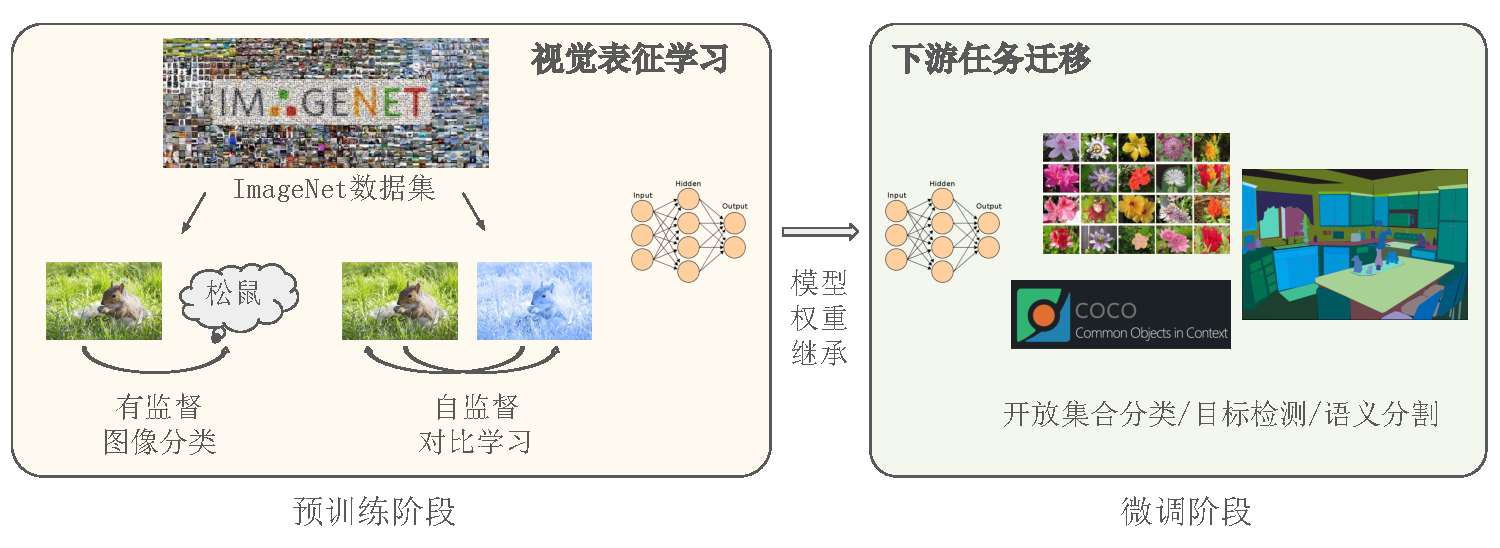
\includegraphics[width=1.0\linewidth]{figures/论文-图1-预训练-微调-v2.pdf}
  \caption{“预训练-微调”方法示意图}
  \label{fig:1-pt-ft-example}
\end{figure}

随着深度学习的发展,数据驱动已成为计算机视觉系统构建的重要范式。然而,获取大规模高质量的视觉任务标注数据需要耗费大量人力物力。为解决这一问题,研究人员提出“预训练-微调”方法。通过解耦通用视觉表征学习与下游任务迁移过程,“预训练-微调”方法有效缓解了任务数据收集难、标注贵的难题,提升了模型的性能表现。
% 如图\ref{fig:1-pt-ft-example}所示,预训练阶段通过大规模数据和代理任务驱动模型习得具有良好泛化能力的视觉表征,而微调阶段通过权重迁移实现模型对下游任务的适应。
“预训练-微调”方法如图\ref{fig:1-pt-ft-example}所示。在预训练阶段,模型基于ImageNet\cite{deng2009imagenet}等大规模基准数据集,通过有监督图像分类代理任务\cite{alexnet}或自监督对比学习代理任务\cite{chen2020simple}习得具有良好泛化能力的视觉表征。在微调阶段,通过模型权重继承和下游任务迁移方法,预训练模型在MSCOCO目标检测和识别任务\cite{chen2015microsoft}、ADE20K语义分割任务\cite{zhou2019ade}等视觉任务上进一步学习。
“预训练-微调”方法显著提升了视觉任务的数据使用效率和性能表现,已经成为计算机视觉领域的重要范式。
% “预训练-微调”范式将通用表征学习和任务能力培养拆分成两个阶段,显著提升了模型在各类下游任务上的数据利用效率和性能指标,缓解了下游任务数据收集难、标注贵的困境。
% “预训练-微调”范式促进了大语言模型和相关应用的发展与落地,但实现对物理世界通用感知的视觉模型研究进展仍较缓慢。人工智能领域的莫拉维克悖论\cite{mindchildren}阐明:“要让电脑如成人般地下棋是相对容易的,但是要让电脑有如一岁小孩般的感知和行动能力却是相当困难甚至是不可能的。”这一悖论也反映了视觉模型预训练研究的巨大挑战。% 需要从并列讲述视觉和语言过渡到视觉

% 0318,感觉还差一段描述视觉任务语义性的;但不知道加到哪里比较合适
% 视觉任务的本质是将像素级的图像信息映射到语义概念空间进行理解和推理。这一过程需要系统掌握从低层次的边缘、纹理特征到高层次的场景理解等多个层面的语义表达。由于视觉表征与语义概念之间存在显著的鸿沟,相同语义可能呈现出显著的视觉差异,而不同语义概念却可能具有相似的视觉表现。

% 难点-语义;标注依赖/跨任务泛化弱/细粒度建模不足
% 监督学习→封闭语义空间
% 自监督学习→无语义指引
% 共同缺陷→视觉单模态局限
% 解决方案→跨模态语言监督
视觉任务的核心挑战在于实现从像素级感知特征到语义级认知概念的有效映射。无论是图像分类、检测还是分割任务,都需要模型理解图像中物体、场景的语义内涵,并建立起视觉表征与抽象概念之间的关联。这种语义理解能力直接影响模型在开放环境下的泛化表现。
然而,当前主流的视觉预训练方法在语义理解层面仍有双重困境:基于图像分类的有监督预训练受限于封闭语义空间和稀疏标注信息,而基于图像自身的自监督预训练的视觉特征停留在感知层面,无法建立有效的语义理解能力。
具体而言,有监督图像分类方法通过人工标注的类别标签建立视觉感知到语义理解的映射,但其封闭式的类别空间导致模型语义覆盖狭窄,而独热标签监督信号的语义稀疏性迫使模型建立粗粒度的图像-语义关联,牺牲了模型在开放环境下的概念泛化能力。此外,人工标注的数据成本限制了图像分类数据的大规模扩展。
% 此外,作为预训练代理任务,图像分类任务的监督信号较为稀疏,因此在预训练过程中容易出现模型过拟合现象,从而限制了模型习得表征的通用性。
% ImageNet分类预训练通过人工标注的类别标签建立视觉-语义映射,但其封闭式词汇表(1000-21K类别)导致语义覆盖狭窄。据JFT-300M研究显示,扩展至3亿标注图像仅能新增1.8%的细粒度概念,边际效益递减显著(Sun et al., 2017)。更严重的是,单热点标签(one-hot label)的监督信号存在语义稀疏性——ImageNet中每张图像仅关联1.05个语义概念(Deng et al., 2009),迫使模型建立粗粒度的类别决策面,牺牲了开放环境下的概念泛化能力。
自监督学习方法通过实例判别、掩码建模等基于图像内在结构的代理任务避免了对数据标注的依赖,但其学习目标局限于图像感知层面的空间连续性、平移不变性等统计特性,难以建立视觉表征与语义概念的关联。
% 这两种视觉预训练方法本质上都未能突破视觉单模态训练导致的模态孤岛效应,无法构建低层特征感知到高层开放语义理解的完整认知过程。
这两种视觉预训练方法本质上都局限于单一视觉模态的信息范围,因此难以构建从低层特征感知到高层开放语义理解的完整认知过程。
% 则可以大规模利用无标注的图像数据,避免了对数据标注的依赖,同时通过图像的空间连续性、平移不变性等特性驱动模型学习可泛化视觉表征,缓解了模型预训练过拟合的问题。然而,自监督预训练方法缺少对语义的建模,通过这种方法得到的模型无法理解语言信息。% 有点牵强的感觉。
% 自监督学习的语义失焦。虽然MoCo、BYOL等方法通过实例判别等代理任务突破标注依赖,但其学习目标局限于图像内在统计特性(如空间连续性、几何不变性)。实验表明,SimCLR在PASCAL VOC多标签分类任务中的平均查准率较监督预训练低14.7%(Chen et al., 2020),暴露其语义建模缺陷。这类方法构建的视觉表征缺乏与语言语义的系统性对齐,导致下游任务难以实现跨模态的知识迁移。
% 早期监督学习范式依赖ImageNet等标注数据集,通过图像分类任务学习语义映射。尽管该范式催生了ResNet等经典模型,但其标注依赖性和封闭类别空间导致表征的语义丰富性和迁移能力受限。随后的自监督学习(如MoCo、SimCLR)通过利用图像内在结构缓解标注依赖,但这类方法在高层语义建模上存在固有局限——旋转预测等代理任务难以建立视觉概念与开放语义的关联,导致模型在细粒度任务中出现语义失配。
% 这两种范式本质上都未能突破视觉单模态的语义隔离——监督学习受制于人工定义的封闭语义空间,自监督学习则困在无语义指引的特征空间。要构建开放语义的视觉智能,亟需引入语言模态的监督信号,通过跨模态对齐建立视觉概念与语言语义的动态连接。

% 曙光-自然语言
% NLP领域预训练模型的成功
% 大规模语言模型带来的启发
% 语言具有更丰富的语义信息+开放词汇
与此同时,自然语言处理领域研究通过大规模自监督预训练方法\cite{BERT,gpt2}在语义理解方面取得了突破性进展,推动了聊天机器人和智能体等应用的快速发展。相比视觉模态,语言模态具有天然的语义优势:它直接编码人类的认知概念,结构化表达能力强、语义泛化性优秀。语言模型在语义理解方面的成功,引发了研究者对视觉表征学习的思考:能否借鉴语言模态的优势来增强视觉表征的语义理解能力?
事实上,神经科学研究表明人脑在视觉信息和语言信息的获取和认知构建过程中展现出深层的协同机制\cite{bemis2013basic},例如角回脑区就同时参与了视觉场景解析和语义概念提取任务。这种认知层面的协同机制,为利用语言作为视觉表征学习的语义先验提供了生物学依据。近年来,一些研究\cite{desai2021virtex,sariyildiz2020learning}已经探索了基于自然语言监督的视觉表征学习方法,并取得了初步进展。

% CLIP,引出需要前面更多过渡!
% 认知科学升维
%     引入fMRI神经影像证据强化理论创新性
%     通过t-SNE可视化建立方法可解释性
% 技术细节深化
%     明确模型架构细节(双塔/编码器类型)
%     量化关键实验指标(准确率/Recall@1)
%     列举典型应用框架(VIMA/DALL-E 2)
% 学术严谨性增强
%     补充图示引用(架构图/可视化图)
%     标注关键性能提升百分比
%     使用皮尔逊相关系数量化神经相似性
% 应用价值具象化
%     区分基础研究(认知模型)与应用领域(生成/具身/工业)
%     采用"方法论支撑"替代模糊的"促进发展"表述
% CLIP 通过“词的向量空间”和“视觉的向量空间”对齐,把视觉表征嵌入到语言所描述的概念中。
% 相比传统方法,它的优势在于:语义开放性(open vocabulary classification)+ 高效跨模态检索 + 强大的零样本能力。

语言-图像对比学习方法\cite{radford2021learning}(Contrastive Language-Image Pre-training,CLIP)作为从自然语言监督中学习视觉表征的里程碑方法,通过在混合图文数据中匹配正样本对实现跨模态表征对齐。这种方法将自监督对比学习思想扩展为多模态数据对比学习方法,在双塔架构中同步优化视觉模型\cite{dosovitskiy2020vit,resnet}与语言模型\cite{Transformer}最大化配对图文样本的互信息,有效利用互联网中的大规模图文对数据构建了感知与语义的统一空间。
% ,通过多模态对比学习的思想,利用互联网规模的图文对数据进行预训练,实现了视觉表征与语言表征的对齐。这种方法有效利用了互联网中大量存在的图文对数据,解决了预训练数据可扩展性的问题。与此同时,该方法有效利用了文本信息对语义进行建模,赋予模型理解语言信息的能力。
% 通过语言-图像对比学习方法预训练得到的模型有效对齐了视觉表征和语言表征,使得相关表征间的距离更近,不相关表征间的距离更远。
通过文本监督信号,CLIP方法将图像分类任务中通过封闭类别空间表示的语义概念扩展至自然语言的开放词汇集合,得到的CLIP模型在零样本开放集合图像识别任务上表现出色。通过可大规模扩展的互联网图文对数据,CLIP方法在视觉表征学习中注入了丰富语义先验,有效对齐了视觉表征与语言表征,可以高效实现零样本图文跨模态检索任务。
% 因此,这种模型无须微调,就可以被用于零样本图文跨模态检索任务中,同时也可以出色完成零样本开放集合图像识别任务,能有效增强搜索引擎的图文检索效果。
% 同时,通过语言-图像对比学习方法预训练得到的视觉模型具有更出色的语义信息理解能力,经过权重迁移到下游视觉任务时,增强了目标检测、语义分割等任务上的物体识别能力,从而进一步推动视觉模型研究的发展与进步。
CLIP方法催生一系列下游任务迁移研究:在图像生成领域,CLIP模型引导的扩散模型\cite{dall-e2}通过文本语义实现保真度高、准确性强的图像合成;在具身智能领域,CLIP模型作为多模态交互的认知基座\cite{llava},赋予了大语言模型视觉感知能力。
作为一种视觉-语言深度结合的预训练方法,CLIP方法已经成为“预训练-微调”范式中的重要一环,为构建通用人工智能的感知系统提供了关键支撑。
% 最近,研究发现语言-图像对比学习方法预训练的模型还可被用于基于文本的图像生成任务,同时也是赋予大语言模型视觉感知能力方法中的重要组成部分,促进了人工智能生成内容领域的繁荣。
% 因此,语言-图像对比学习方法因其可靠的数据可扩展性和对视觉信息与语言信息的有效建模能力,已经成为“预训练-微调”范式中的重要一环。


% 从领域发展过渡到实际科学研究,并提出pt-ft范式;
% 图一:左图预训练(需要上:图像)(下:文本)(左:有监督)(右:自监督);迁移;右图微调(上:图像)(下:文本)

% \todo{需要如何引出有监督和自监督,从而方便后文过渡到语言监督的视觉模型?}这里先不提,主要讲VL,可以较快引出CLIP,落回V之后再重提V的有监督等等

%%%
% 讨论联合微调的范式
% 主要引出解决多模态任务
%%%
% 总:近年来有相当多的工作考虑将两者当作已存在的独立模块,将其组装起来「使用联合微调」处理一系列VL的任务(这里可以扯一些应用,caption,grounding,qa等等),也就是说,他们使用各自领域的预训练,再将两部分模块组装「可以讲一下稍微现代点的VL-BERT系列?」;这种方案受限于原来各自预训练的好坏;
% 图二:可能是图一的延展,为了说明有联合微调,但是很少有联合预训练。注意需要迁移两部分权重。严格起见为了区分VL-BERT,可以把VL-BERT加入一个中间阶段,叫联合对齐?(预训练-对齐-微调)
% \begin{figure}
%   \centering
%   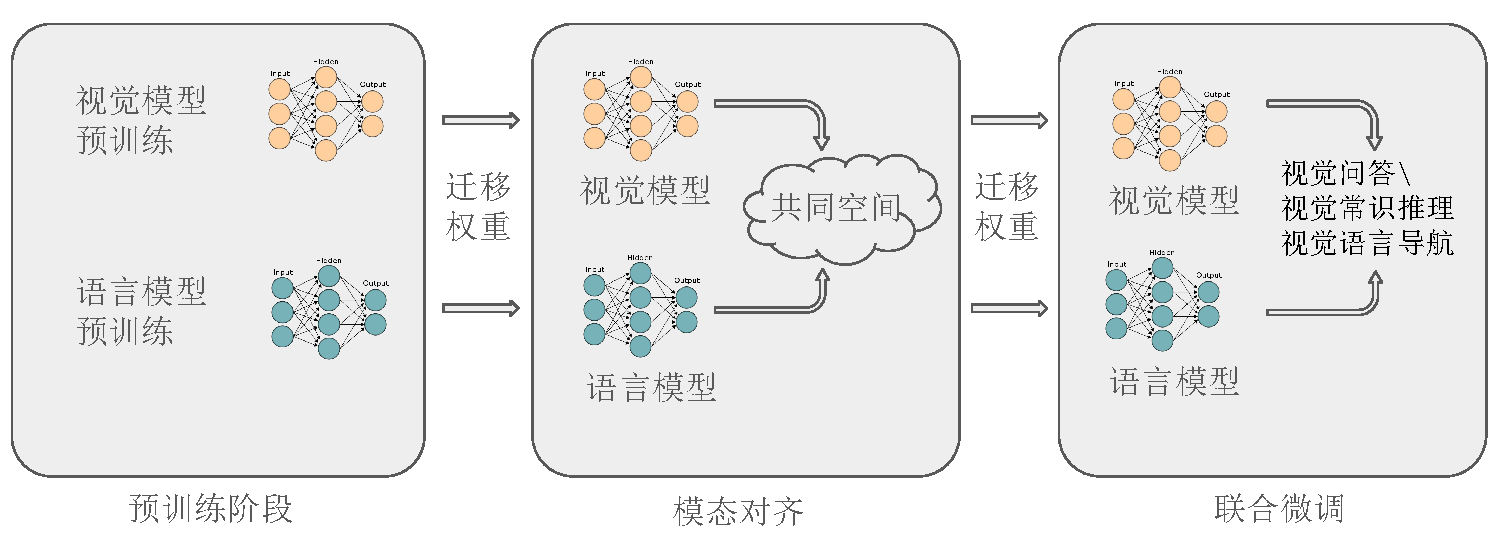
\includegraphics[width=1.0\linewidth]{figures/论文-图2-预训练-模态对齐-联合微调.pdf}
%   \caption{``预训练-模态对齐-联合微调''范式示意图}
%   \label{fig:2-pt-align-ft-example}
% \end{figure}
% 这种``预训练-微调''范式也被推广到了需要同时处理两种信息的多模态任务中,并出现了一种新的阶段:联合微调。如图\ref{fig:2-pt-align-ft-example}右侧所示,联合微调阶段是对微调阶段的扩展。该阶段分别继承预训练阶段得到的视觉和语言模型,在引入额外机制进行架构整合和信息融合后,在视觉问答、视觉常识推理、视觉语言导航等多模态任务数据上微调,以完成相应任务。
% 随着视觉-语言交叉领域的发展,研究人员在``预训练-微调''范式中引入了一个中间阶段,称为模态对齐阶段。如图\ref{fig:2-pt-align-ft-example}中间所示,这一阶段是一种过渡阶段,其形式与预训练阶段类似,使用相对规模较大的多模态通用数据集对预训练阶段得到的单模态模型权重进行联合训练。这一阶段的主要目的是对齐语言的语义空间和视觉的感知空间,从而进一步提升模型在联合微调阶段的数据利用效率和性能指标。
% 联合微调阶段和模态对齐阶段的提出,促进了视觉-语言交叉领域的发展,催生了大量多模态场景和应用。

% 但是追本溯源,``预训练-微调''范式中的关键阶段在于预训练。因为微调阶段受限于数据标注成本高昂,获取难度大,无法扩大训练规模,而预训练阶段可以利用大量无标注或弱标注数据。
% 此外,微调阶段数据形式和目标相对确定,调整空间有限,而预训练阶段数据来源多样,代理任务设计更加灵活,提供了更大的提升空间。
% 同时,提升通用性是人工智能研究的长期追求。增强模型预训练阶段获得的能力,弱化微调阶段的重要性,是一个重要方向\cite{gpt3,gpt4}。
% 因此,越来越多的工作重点转向了预训练阶段的数据挖掘和方法设计。

%%%
% 视觉-语言的联合在认知学、心理学、脑科学等的支持,特别地引出具身智能学说
%%%

% 参考:具身假说:在大脑内部,思维是由负责视觉、行动和情感的同一套神经结构完成的,如果我们想要赋予语言意义,就要借助“感觉—运动”(sensory-motor)系统和情感系统,这些系统负责定义目标和想象、识别,以及付诸行动。进入21世纪后,越来越多的证据表明:心智与身体密不可分。。。。 具身革命业已证明,我们人性的本质、我们思考以及使用语言的能力,根本就是我们的身体与大脑合作的成果。人类心智的运作方式,从思想的本质到我们理解语言含义的方式,都与身体紧密相连,与我们在这个世界的觉察、感受与行动有关。我们不是冷血的思考机器,生理学为哲学提供了概念基础。
% 参考:具身模拟假说: 认为语言理解是人在心智中基于自己过去的视觉、听觉、运动等体验进行的模拟。具身模拟假说拥有大量认知科学、脑科学、语言学等学科的实验结果作为支持。。。人对语言的理解离不开身体与外界环境的互动,只有通过身体的视觉、听觉、运动等方面的经验积累才能实现对语言的理解,因此,有人认为脱离身体的语言理解是不可能实现的。在我看来:人工智能或自然语言处理的终极目标不应该是模仿人类,而应该是为人类提供有用的工具。从这个意义上来说,我们没有必要完全复制人类的语言理解过程,实际上,参考人类的处理机制,实现接近人类的语言处理能力应该就已足矣。
% 总:少有工作从源头上考虑两个模态共同预训练的可能。两者都有从互相模态信息中提取能力的可能(提一下之前BERT don't know how many legs of birds && Vision 一直使用受限Semantic Space的历史,泛化能力也会受label粒度影响(比如自然文本可以标蓝色衣服红色裤子小人,但是原来那种fix label set的只能标人,认识人但不认识腿之类))。

% ref: https://airs.cuhk.edu.cn/article/1124
% 随着人类对智能的理解进一步深入,越来越多观点认为智能是人类整个身体结构的综合表现,也即视觉的感知和语言的理解密不可分。研究人员也提出了相关的具身假说\cite{understand, embodiment}。% Embodiment Hypothesis
% 具身假说认为,人类在大脑内部构建语言意义,是通过处理视觉、行动等功能的同一套神经结构完成的,也就是说,人类通过感知-运动-想象系统来理解语言意义。
% 进入21世纪后,有越来越多的脑科学、心理学和行为学的证据表明人的思维和感知密不可分,语言的意义无法脱离身体的感知进行构建,而语言又是表达感知、做出行动的重要方式。
% 无独有偶,在视觉预训练和语言预训练领域也都发现了类似的现象:缺乏语言引导的有监督视觉预训练方法通过无语义的类别分类作为代理任务,导致模型跨类别集合的泛化较为困难,限制了模型的迁移效果\cite{imagnettransfer};而纯语言预训练模型则可能在物理世界的常识问题上产生幻觉\cite{numersense}。

%%%
% 引出视觉-语言联合预训练的范式
% 落脚到视觉需要语言(怎么反驳不会语言的狗也有视觉能力!)
%%%
% 总:特别地,Vision model需要language才能对齐人类描述,所以Vision needs language more「这里要斟酌一下过渡,以及要不要提这也是本文的主要研究内容。」
% 参考:从演化认知的角度,这种跨模态协同机制可能源于早期人类的社会协作需求——当原始人类开始使用工具和构建居所时,必须通过语言符号将三维空间关系(视觉维度)转化为可传递的操作指令(语言维度)。这种进化压力促使大脑发展出独特的双通道处理架构:视觉系统负责建立实体世界的心理模拟,而语言系统则构建抽象符号的逻辑框架,二者通过前额叶皮层的高级调控实现动态耦合[6]。
% 图三:左图联合预训练(囊括模态对齐),右图分为三个部分(各自微调和联合微调);把各自微调加上是为了强调关注vision task!
% \begin{figure}
%   \centering
%   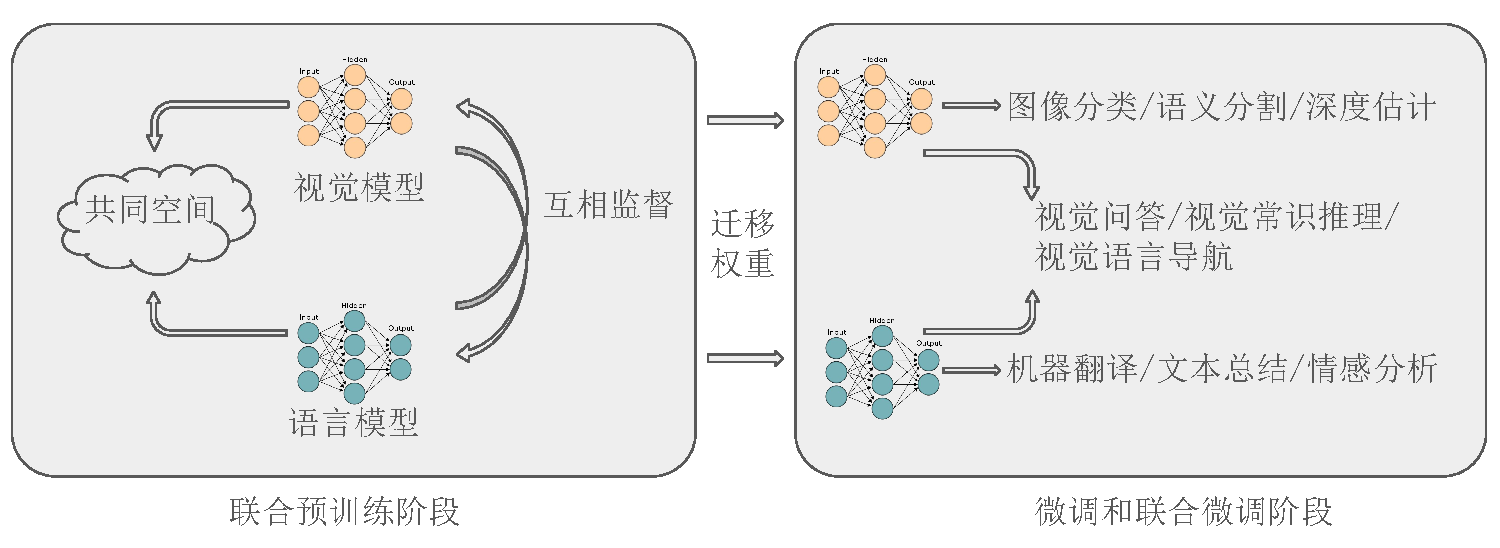
\includegraphics[width=1.0\linewidth]{figures/论文-图3-联合预训练-微调.pdf}
%   \caption{``联合预训练-微调''范式示意图}
%   \label{fig:3-fusept-ft-example}
% \end{figure}
% 认知神经科学的发现和人工神经网络的进展都展现了在预训练阶段同时处理视觉和语言信息,并从另一模态中学习的巨大潜力。在本文中,这一阶段被称为联合预训练阶段。
% 如图\ref{fig:3-fusept-ft-example}所示,这种方法将原本独立的视觉、语言预训练阶段合并,让视觉信息和语言信息互相监督,同时在预训练阶段完成原本模态对齐阶段的任务,无需引入额外的过渡环节,从而可以进一步统一和简化学习范式。
% Transformer\cite{Transformer}模型架构因其在图像信息建模\cite{dosovitskiy2020vit,Swin}与文本信息建模\cite{BERT,gpt2}任务上的出色表现,已经逐渐代替了原先有针对性设计的卷积神经网络和循环神经网络。Transformer网络从模型架构层面进一步统一了两种模态的处理方式。

% 但是长久以来,尚未找到足够高效,且有较强扩展性的“联合预训练”方法。
% 对人的生理、行为和智能理解支持了多模态“联合预训练”的出发点。这种方式从根本上从互相信息中学习,有更强的建模上限balabala。
% 视觉信息通过与语言系统的动态交互,形成了人类特有的符号表征能力。

% 回到从视觉模型的主体出发,因为CLIP本身就是这样的落脚点:Learning Transferable Visual Models From Natural Language Supervision
% 这里从联合收束避免讨论语言任务微调什么的还是比较重要的。
% 近年来大语言模型的成功\cite{gpt3,gpt4,palm,dsv3,chinchilla},以及视频生成模型在建模物理世界规律时遇到的挑战\cite{kang2024farvideogenerationworld},都在强调莫拉维克悖论(Moravec's Paradox)的正确性。
% 人类觉得更代表高级智能的数学、代码、写作等能力反而是当前人工智能领域进展较快的方向,而普遍认为对人类来说简单的任务,比如图像识别、运动理解、肢体行动等任务则进展缓慢。
% 这种发展速度的不一致性限制了当前人工智能系统的大规模应用。因此本文以视觉-语言联合预训练方法中的\textit{视觉模型}为主要关注点,进一步研究联合预训练的方法,并关注下游视觉任务和视觉-语言多模态任务的迁移效果,以期促进相关领域的进一步发展。

\section{语言-图像对比学习方法介绍及其研究目标}
本节主要介绍了语言-图像对比学习方法的基本原理与研究目标。第\ref{sec:clip-introduce}节首先介绍了从早期基于人工标注数据的语言监督视觉表征训练方法,到借鉴视觉自监督对比学习思想的技术演进,并介绍了CLIP方法的具体实现方式,分析了CLIP方法在利用大规模互联网图文对数据方面的优势。第\ref{sec:clip-target}节分析了CLIP方法的两个主要研究目标:一是通过降低数据中语义噪声、扩展语义信息源来提升预训练视觉表征的语义理解能力,二是设计有效的迁移策略以增强模型在细粒度视觉任务和语义生成任务上的性能表现。

\subsection{语言-图像对比学习方法的发展与介绍}
\label{sec:clip-introduce}
% 先介绍一下语言-图像对比学习数据 % 可以画个这类数据的获取图
基于自然语言监督的视觉表征学习方法需要大规模的图文对训练数据。早期方法主要依赖众包平台(如亚马逊土耳其机器人\cite{AMT})收集人工标注的图像描述数据\cite{young2014flickr, chen2015microsoft}。这种方式虽然标注质量高,但数据收集成本昂贵、规模受限。语言-图像对比学习方法另辟蹊径,转向利用网页中的图像替代文本(Alternative Text)构建大规模训练数据\cite{YFCC100M, sharma-etal-2018-conceptual, changpinyo2021conceptual}。这些替代文本是网页代码中表述图像内容的文本属性,可以用于在图像无法显示时向视觉障碍用户传达图像内容,或供搜索引擎建立图文索引,因此天然包含了对图像内容的丰富语义描述。这种基于互联网数据的构造方式具有显著优势:数据收集成本低、来源丰富多样、语义覆盖广泛,且可以持续扩展数据规模。

% 早期基于自然语言监督的视觉表征学习方法过渡,为了进一步引出视觉对比学习方法
早期基于自然语言监督的视觉表征学习方法主要依赖人工标注的高质量图像描述数据集\cite{young2014flickr, chen2015microsoft}进行训练。基于这类数据的特点,这些方法主要借鉴了自然语言处理领域的成功经验。一类方法扩展了掩码语言模型\cite{BERT}的思想,通过要求模型利用图像信息预测被掩码文本内容来学习视觉表征\cite{sariyildiz2020learning}。另一类方法借鉴自回归语言模型\cite{gpt2}的设计,利用马尔可夫性质,基于图像信息逐步生成完整的文本描述\cite{desai2021virtex}。这些方法强调图像与文本之间的严格对应关系,要求文本准确、完整地描述图像内容。然而,这种严格的数据假设限制了这些方法在互联网图文对数据上的应用:网络数据中的文本描述往往包含噪声或不完整内容,且与图像的对应关系较为松散。这促使研究者思考一种更适合处理大规模、噪声化互联网图文数据的表征学习方法。

% 先介绍视觉模型自监督对比学习方法,为后续介绍CLIP方法提供铺垫
为了应对互联网图文对数据的噪声特性,语言-图像对比学习方法\cite{radford2021learning}借鉴了视觉自监督对比学习的核心思想。视觉自监督对比学习方法\cite{chen2020simple}基于图像的空间连续性、平移不变性等性质,对输入图像应用颜色变换、缩放裁剪、翻转旋转等数据增强策略,生成同一图像的不同视角。这种方法将来自同一原始图像的增强样本对定义为正样本对,将不同原始图像的增强样本之间的配对定义为负样本对。通过最大化正样本对间视觉表征的相似度,同时最小化负样本对表征的相似度,模型学习到具有感知一致性的视觉表征。
% https://zhuanlan.zhihu.com/p/370782081
对比学习方法的关键优势在于它通过建模样本间的相对关系来学习表征。即使部分样本带有噪声,只要能保持相似样本的表征相对更接近、不相似样本的表征相对更远离这一基本相似度排序关系,模型就能学到区分性较好的有效表征。这种基于相对关系的学习策略提升了方法对数据噪声的容忍能力。

\begin{figure}
  \centering
  % \subcaptionbox{语言-图像对比学习方法概览\label{fig:6-CLIP-Method}}
  %   {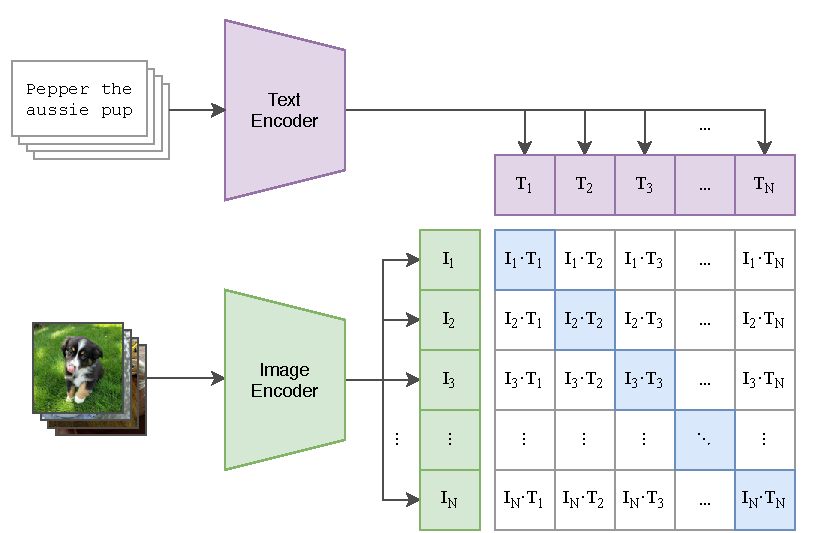
\includegraphics[width=0.48\linewidth]{figures/论文-图6-CLIP-方法.pdf}}
  % \subcaptionbox{语言-图像对比学习方法扩展性分析\label{fig:6-CLIP-Scaling}}
  %   {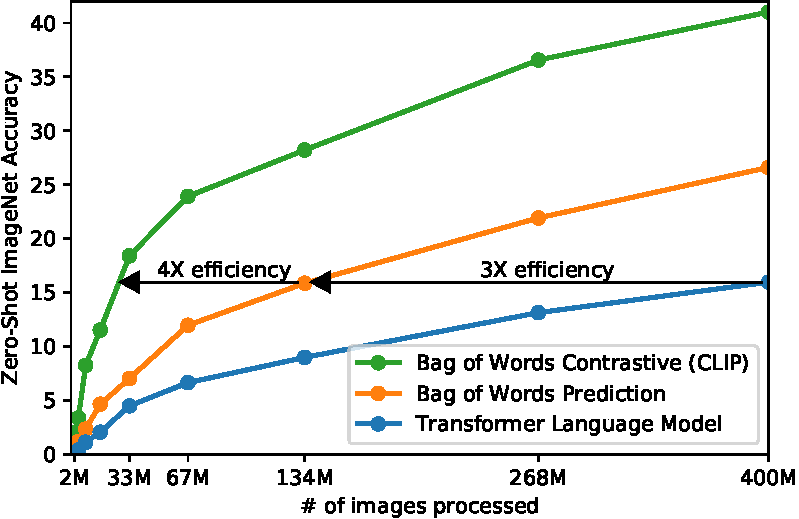
\includegraphics[width=0.48\linewidth]{figures/论文-图6-CLIP-效率.pdf}}
  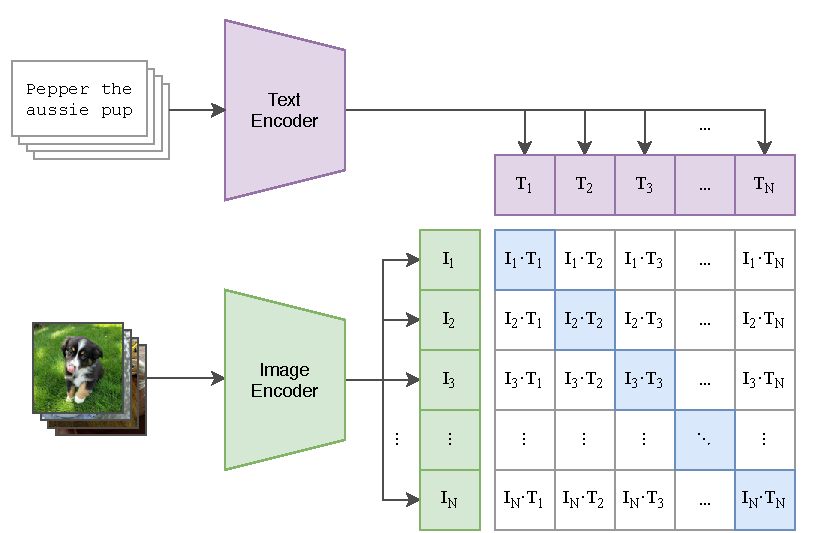
\includegraphics[width=0.9\linewidth]{figures/论文-图6-CLIP-方法.pdf}
  \caption{语言-图像对比学习方法\cite{radford2021learning}概览}
  \label{fig:6-CLIP-Method}
\end{figure}

% 正式引出CLIP
% 互信息:https://www.bilibili.com/opus/776589765893947474 或者 https://zhuanlan.zhihu.com/p/583078368
% 通过最大化配对图文样本的互信息\cite{hjelm2018learning}
语言-图像对比学习方法创新性地将对比学习思想扩展到跨模态场景,从而有效利用带有噪声的大规模互联网图文数据,并从中提取有效的语义信息进行视觉表征学习。
具体而言,CLIP方法将配对的图像和文本视作对同一物体或场景的不同模态描述,构建正样本对;而将不配对的图像和文本视作描述不同物体或场景的负样本对。与视觉自监督对比学习类似,CLIP方法在图像表征与文本表征的共同空间中,拉近描述同一内容的跨模态表征,同时推远描述不同内容的跨模态表征。
如图\ref{fig:6-CLIP-Method}所示,给定一组$N$张图像$\mathcal{I}=\{I_1,\cdots,I_N\}$及其对应的文本描述$\mathcal{T}=\{T_1,\cdots,T_N\}$,CLIP方法的核心目标可以形式化为最小化如下比值:
\begin{equation}
    \min_{\theta}\frac{\sum_{i=1}^{N}f_{\theta}(I_i,T_i)}{\sum_{i\neq j;i,j\in[1,N]}f_{\theta}(I_i,T_j)},
    \label{eq:instance-level}
\end{equation}
其中$f_{\theta}$ 为距离度量函数。在实际实现中,CLIP方法构造了一个双塔架构同时训练视觉模型$\theta_I$和语言模型$\theta_T$来提取双模态表征,并采用InfoNCE损失函数\cite{oord2018representation}优化模型:
\begin{equation}
 \mathcal{L}_{I2T}=-\frac{1}{N} \sum_{i=1}^{N} \log \frac{\exp \left(\frac{\cos \left(\theta_I(I_{i}), \theta_T(T_{i})\right)}{\tau}\right)}{\sum_{j=1}^{N} \exp \left(\frac{\cos \left(\theta_I(I_{i}), \theta_T(T_{j})\right)}{\tau}\right)},
 \label{eq:infonce}
\end{equation}
其中$\cos(\cdot, \cdot)$表示表征间的余弦相似度,$\tau$为温度参数,用于调节正负样本对的对比强度。以文本为查询的对比损失$\mathcal{L}_{T2I}$形式类似,仅需交换图文表征位置。
从公式\eqref{eq:infonce}可以看出,CLIP方法通过优化图文样本对之间的相对距离来驱动学习。这种相对度量的机制使得CLIP方法对图文对之间的严格对应关系要求较低。同时,通过温度参数$\tau$的调节,模型可以灵活控制表征对齐的程度。这种设计使得CLIP方法相比于其他基于自然语言监督的视觉表征学习方法更适合处理互联网图文数据:它不要求文本严格描述图像内容,而是通过对比学习框架来捕捉不同模态表达之间的语义关联,从而能够更好地利用大规模但噪声化的互联网图文数据进行预训练。

% 语言-图像对比学习方法借鉴了这种思想,并将其推广到图文对数据中。具体而言,语言-图像对比学习方法将配对的图像信息与文本信息视作对同一物体或场景的不同描述视角,因此将它们称为正样本对,而将不配对的图像信息与文本信息视作描述了不同物体或场景的负样本对。
% 与实例级对比学习方法类似,语言-图像对比学习方法构建了一个图像表征与文本表征的共同空间,聚合描述同一物体的不同模态表征,分散描述不同物体的不同模态表征。
% 如图\ref{fig:6-CLIP-Method}所示,将一组$N$张图像记作$\mathcal{I}=\{I_1,\cdots,I_N\}$,将对应的一组$N$条文本记作$\mathcal{T}=\{T_1,\cdots,T_N\}$,并记模型参数为$\theta$,语言-图像对比学习方法可以被理解为最大化如下训练目标:
% \begin{equation}
%     % \max_{\theta}\sum_{i=1}^{N}\left[\log(f_{\theta}(I_i,T_i))-\sum_{j=1}^{N}\log(1-f_{\theta}(I_i,T_j))\right],
%     \min_{\theta}\frac{\sum_{i=1}^{N}f_{\theta}(I_i,T_i)}{\sum_{i\neq j;i,j\in[1,N]}f_{\theta}(I_i,T_j)},
%     \label{eq:instance-level}
% \end{equation}
% 其中$f_{\theta}$为距离度量函数。通常而言,语言-图像对比学习方法会同时训练一个视觉模型$\theta_I$和一个语言模型$\theta_T$来分别提取图像表征和文本表征,并用表征间的余弦距离作为距离度量方法。
% 因此在实际的训练过程中,语言-图像对比学习方法采用InfoNCE损失函数\cite{oord2018representation}驱动模型训练:
% \begin{equation}
%  \mathcal{L}_{I2T}=-\frac{1}{N} \sum_{i=1}^{N} \log \frac{\exp \left(\frac{\cos \left(\theta_I(I_{i}), \theta_T(T_{i})\right)}{\tau}\right)}{\sum_{j=1}^{N} \exp \left(\frac{\cos \left(\theta_I(I_{i}), \theta_T(T_{j})\right)}{\tau}\right)},
%  \label{eq:infonce}
% \end{equation}
% 其中$\cos(\cdot, \cdot)$表示图像表征与文本表征之间的余弦相似性。$\tau$表示温度超参数,控制了训练过程中正样本对与负样本对间的区别程度。式\eqref{eq:infonce}展示了语言-图像对比学习方法中以图像为中心与其他文本间的对比学习损失函数$\mathcal{L}_{I2T}$,而以文本为中心的对比学习损失函数$\mathcal{L}_{T2I}$则形式上与$\mathcal{L}_{I2T}$一致,只需要交换图像表征与文本表征的位置,这里不再赘述。

% 从式\eqref{eq:infonce}可以看出,语言-图像对比学习方法通过优化图文正样本对和负样本对间的相对距离驱动模型学习,并用温度超参数$\tau$来控制目标相对距离的幅度。这种方法对图像与文本信息一一对应的数据假设依赖较弱,并通过对比学习方式对齐了图像集合$\mathcal{I}$的表征空间和文本集合$\mathcal{T}$的表征空间。
% 因此,语言-图像对比学习方法更符合互联网中易收集的图文对数据的实际特性。相比于前述的视觉-语言多模态预训练方法,这种方法在扩展预训练数据时效率更高,可供学习的语义信息更为充足。

% 如图\ref{fig:6-CLIP-Scaling}所示,语言-图像对比学习方法\cite{radford2021learning}(绿色线)在ImageNet-1K数据集\cite{deng2009imagenet}零样本图像识别任务上相比于有监督图像分类方法(橙色线)有3倍的数据利用效率提升,而相比于从文本标注中学习视觉表征方法(蓝色线)则有11倍的数据利用效率提升。
% 天然提供了一项额外好处:\todo{简单的大规模检索算法和零样本开放集合识别} % 开放集合识别貌似基于回归的办法也可以做。可以提检索简化了识别(把open end的映射问题转为排序问题),对物体检测、语义分割都有帮助
% 因此,以语言-图像对比学习方法为核心的视觉-语言多模态预训练方法具备高效的数据利用能力和大规模数据扩展的潜力,同时通过对比学习的方式充分利用图文对中的语义信息,对齐了视觉表征与语言表征,已经成为重要的视觉-语言多模态预训练方法。

\subsection{语言-图像对比学习方法的研究目标}
\label{sec:clip-target}
% pt
作为一种新型的视觉表征学习方法,CLIP方法利用大规模互联网图文对数据进行预训练,具有显著的数据可扩展性优势,但同时也面临着图文对数据质量参差不齐的挑战。尽管CLIP方法通过对比学习思想在一定程度上缓解了这个问题,放宽了文本严格描述图像内容的要求,但要提取有效的语义信息仍然需要保证图文对之间相似度的相对排序关系。因此提升语义信息质量,增强视觉表征与语言表征的对齐效果,成为CLIP方法研究的重要目标之一。
% 此外,与传统视觉预训练方法相比,CLIP方法的核心创新在于借助语言模态强大的语义表达能力来指导视觉表征学习。
% 这种思路启发了进一步的思考:能否将计算机视觉领域积累的丰富标注资源转化为语言可建模的形式,作为对互联网图文数据的有效补充?这些视觉标注涵盖了多个层次和不同描述角度的图像信息:从细粒度的物体标注(如目标检测的边界框、语义分割的像素类别、实例分割的物体轮廓),到中观层次的物体间关系(如空间位置关系、物体交互方式),再到宏观层面的场景语义理解(如场景类别、事件描述)。这些多层次、多维度的视觉标注信息为图像内容提供了丰富的语义描述。
% 将这些已有的结构化视觉标注转化为自然语言形式,不仅能为CLIP方法训练提供高质量的语义锚点,增强视觉表征与语言表征的对齐精度,还能扩展图像可用的语义信息来源,突破了CLIP方法对图文对数据形式的依赖限制。
此外,计算机视觉领域积累了丰富的有标注任务数据。这些视觉标注涵盖了多个层次和不同描述角度的图像信息:从细粒度的物体标注(如目标检测的边界框、语义分割的像素类别、实例分割的物体轮廓),到中观层次的物体间关系(如空间位置关系、物体交互方式),再到宏观层面的场景语义理解(如场景类别、事件描述)。这些多层次、多维度的视觉标注信息为图像内容提供了丰富的语义描述。这些数据不仅能为CLIP方法训练提供高质量的语义锚点,增强视觉表征与语言表征的对齐精度,还能扩展图像可用的语义信息来源,突破CLIP方法对图文对数据形式的依赖限制。因此在CLIP方法中有效引入已有的结构化视觉标注信息进行增强也是CLIP方法的重要目标之一,为整合现有视觉数据集提供了新思路。

% 作为一种视觉-语言多模态预训练方法,语言-图像对比学习方法的一个重要研究目标是如何扩展图文对数据、提高图文对数据质量,从而增强视觉表征与语言表征的对齐效果。
% 随着“预训练-微调”范式的发展,研究人员总结出了一条重要的实践规律:扩展定律。针对语言模型中的扩展定律\cite{kaplan2020scaling, gpt4}研究显示,数据规模、模型参数量及两者共同决定的训练计算量是影响预训练方法效果及其在下游任务上迁移表现的重要因素,而数据质量差异和预训练算法设计则影响了扩展效率。扩展定律的提出直接促进了近期大规模语言模型的发展与应用\cite{gpt4,dsv3},而更多其他领域的“预训练-微调”范式研究\cite{henighan2020scaling, aghajanyan2023scaling, xie2023data}也进一步证明了扩展定律的有效性和可推广性。因此,增强语言-图像对比学习方法的预训练可扩展性,提高预训练扩展效率是此类方法的重要研究目标之一。

% ft
在提升预训练数据质量和语义覆盖范围的基础上,改进CLIP方法在下游任务上的迁移性能是另一个关键研究目标,也是"预训练-微调"范式的核心诉求。CLIP方法通过图文对训练实现了视觉-语言表征的对齐,在零样本图文跨模态检索和开放集合图像识别等直接利用跨模态表征对齐性质的任务上展现出优异表现。然而,视觉任务的多样性对预训练模型提出了更高要求:一方面,细粒度视觉任务(如目标检测、语义分割、深度估计等)需要模型具备密集预测和精细感知能力,而CLIP模型在实例级对比学习预训练过程中并未显式学习这些特性;另一方面,早期基于自然语言监督的视觉表征学习方法\cite{desai2021virtex}通过生成式训练,天然具备图像描述生成等语义生成能力,而基于对比学习的CLIP方法则缺乏这种能力。
因此,如何设计有效的迁移方法以扩展CLIP模型的应用范围成为重要研究方向:首先,需要探索能够充分利用CLIP模型强大语义理解能力,同时增强其在细粒度视觉任务上表现的迁移学习策略;其次,需要研究将CLIP模型的判别式表征转化为生成式能力的有效迁移方法,使其能够支持更广泛的视觉-语言生成任务。这些研究不仅有助于提升CLIP方法的实用价值,也为探索通用视觉表征学习提供了新的思路。
% 在具备强可扩展性和高扩展效率基础上,如何提高语言-图像对比学习方法在各类下游任务上的迁移表现也是一个重要的研究目标。
% 前文提到,语言-图像对比学习方法利用图文对数据,对齐了图像表征与文本表征,因此在零样本图文跨模态检索和零样本开放集合图像识别等直接运用图像表征与文本表征对齐性质的任务上表现优异。
% 但是下游视觉任务类型多样,不仅包括ImageNet-1K数据集图像分类、iNaturalist数据集细粒度图像分类、MSCOCO图像描述生成等图像层面的语义理解或生成任务,也包括目标检测、语义分割、深度估计、光流提取等需要密集感知的细粒度视觉任务。
% 如何将语言-图像对比学习方法迁移到各类下游任务,同时广泛地提升其在各类下游任务上的性能表现同样是一项重要的研究目标。



% 视觉语言多模态预训练方法也经过了几个阶段的发展,早期以图像为条件的掩码语言模型比较流行。后来,它被从文本标注中学习视觉表征的方法逐渐替换,因为后者训练过程中的语义信号更加丰富。随着时代的发展,语言图像对比学习方法,也就是clip方法出现,因为这种方法的数据可扩展性更好,因此逐渐成为最重要的视觉-语言多模态预训练方法。

% 字符级联合预训练方法受自然语言处理领域的进展影响很大,其中两项代表工作分别是2020年提出的ICMLM\cite{sariyildiz2020learning}方法和2021年提出的VirTex\cite{desai2021virtex}方法。
% 两者分别是自然语言预训练方法中基于掩码语言词元建模模型BERT\cite{BERT}和基于语言自回归模型GPT\cite{gpt2}的拓展。其中基于自回归模型的VirTex方法(如图\ref{fig:5-character-instance}(a)所示)允许对自然语言监督信号进行充分利用,而ICMLM方法受限于掩码词元的比例不能过大,只能对监督信号的部分内容进行学习。
% 因此基于自回归模型的方法在下游任务上的迁移表现普遍优于基于掩码语言词元建模的方法。
% 这些小规模的研究工作首次证明基于视觉-语言联合预训练方法得到的视觉模型在图像分类、目标检测等下游视觉任务上可以取得良好的性能表现,同时无需额外的模态对齐阶段即可完成诸如图像注释(Image Captioning)等多模态任务,初步展示出视觉-语言多模态联合预训练方法的巨大潜力。

% 引出缺陷,引出CLIP,引出为什么CLIP好
% 达哥的缺陷是先讲了自监督的目标(迁移性好,扩展性强),然后讲实例级这两方面不好(迁移性特指dense tasks)他是先从实例级做起的,然而我上来就是CLIP)
% 随着研究深入,字符级语言监督的训练方法弊端逐渐显现,其中的核心原因是这种训练方法对图文配对数据的质量要求较高。这里将图片记作$I$,将长度为$n$的字符词元序列记作$T=\{t_1,\cdots ,t_n\}$,记模型参数为$\theta$,字符级语言监督方法本质上在最大化如下概率估计:
% \begin{equation}
%     \max_{\theta}\sum_{i=2}^{n}log\left({p_{\theta}(t_i|t_{1:i-1},I)}\right)    
%     = \max_{\theta}log\left({p_{\theta}(t_{2:n}|t_1,I)}\right)
%     \label{eq:character-level}
% \end{equation}

% 因此,此类方法强化了图文对的对应关系,其优化目标最终导向图像与文本的一一配对。
% 然而,这个假设在现实场景中很难成立。一方面文本描述千变万化,本身不存在强对应关系,另一方面这也与互联网数据的特性有关。
% 互联网中的替代文本与弱监督方法中的主题标题类似,虽然大部分是人类所写,但其质量良莠不齐,容易出现占位符、无关文本或低信息文本的情况,标注的信噪比较低。
% 因此,前述提到的两种字符级语言监督预训练方法均只在噪声比例较低的\{图像,文本\}对数据集,如MSCOCO\cite{chen2015microsoft}数据集上有成功应用,难以推广到以互联网替代文本为主的更大规模数据集\cite{sharma-etal-2018-conceptual}。
% 这一点限制了此类方法的可扩展性和方法上限。

\section{语言-图像对比学习方法的挑战与主要研究思路}
\label{sec:instance-challenge}

\subsection{增强预训练数据语义信号质量的挑战与研究思路}
% 缺陷一:数据噪声问题;前面从细粒度过渡过来的时候已经重提了噪声问题,怎么增强这部分的表述呢?泛化性好但是细粒度能力差(参考UniCL figure-6绘图)
预训练数据的规模和质量是影响模型效果的关键因素。互联网图文对数据中的大量噪声影响着对CLIP方法视觉-语言表征的对齐效果。这些噪声主要来源于文本信息的低质量性和不规范性:作为图像的替代描述,网页中的替代文本往往由网页制作者随意编写,缺乏统一的规范要求和严格的质量控制。这导致了多种形式的数据噪声:一方面,不少文本描述与图像内容的语义关联性较低,如仅包含图像的文件名、网页链接或其他元数据信息;另一方面,部分文本可能完全不包含有效语义信息,如重复字符、随机字符串等占位符文本。这些噪声数据不仅无法为视觉表征学习提供有效的语义监督信号,还可能误导模型建立错误的视觉-语言对应关系,降低预训练的效果。更为根本的是,作为一种弱标注的数据来源,互联网图文对数据面临着质量提升与规模扩展的内在矛盾:强化语义质量控制往往意味着更高的获取成本,这将不可避免地限制数据规模的扩展。

针对这一问题,现有工作主要从降低数据噪声出发,提出了多种筛选策略:一类方法基于人工设计的规则(如文本长度、特殊符号比例、固定模式匹配等)进行筛选;另一类方法利用预训练的小规模CLIP模型对数据质量打分进行筛选;还有一些方法尝试利用ImageNet等图像分类数据集作为锚点,通过文本与类别匹配或图像相似度来筛选高质量图文对。然而,这些方法都存在明显局限:基于人工规则的方法依赖专家先验知识,容易出现遗漏或误删;基于CLIP模型打分的方法受限于对比学习的相对度量特性,难以提供可靠的绝对质量评估;基于图像分类数据的方法则受限于分类数据自身的封闭语义空间,限制了图文对数据的语义丰富度。
因此,如何设计有效的噪声控制策略,并探索新的可用语义信息来提升语言-图像对比学习的预训练效果,仍然是一个重要的研究挑战。

基于上述挑战,本文提出了一个新的研究思路:进一步扩展CLIP方法借助语言模态强大的语义表达能力来指导视觉表征学习的核心思想,将其他形式的有标注图像数据转化为语言可建模的形式,并通过对比学习框架实现多源数据的统一建模。具体而言,CLIP方法将配对的图像和文本视作同一内容的不同模态表达,通过对比学习实现视觉-语言表征对齐。这一思路可以推广到更广泛的数据形式:将任何配对的图像与其标注信息都视作对同一语义概念的不同描述视角,从而将各类已有的视觉数据源统一到对比学习框架中。
这种方法具有双重优势:首先,现有的视觉标注数据通常经过严格的人工校验,具有较高的质量保证,将其整合到预训练过程中可以为模型提供准确的语义监督信号,提升预训练数据的整体质量;其次,不同类型的标注数据(如分类标签、检测框、场景类别等)从不同角度和粒度描述了图像内容,这种多样性扩展了模型可获取的语义信息来源。因此,关键问题在于如何选择合适的高质量标注数据,并设计有效的转化机制,使其能够融入对比学习的预训练框架。

% 因此,CLIP方法可以扩展到\{图像,文本,标注\}的三元组。
% 若进一步将标注转化为文本形式,这种\{图像,文本,标注\}三元组可以统一建模为\{图像,替代文本或标注文本\}的形式,使CLIP方法可以深度利用已有带标注的数据源进行训练。
% 考虑到已有数据标注往往经过不同程度的人工校对,且标注粒度有不同层次,信息覆盖角度多样,在一定程度上提升了整体数据的信噪比,因此这种方法对提升CLIP方法预训练过程中的数据效率也有一定帮助。
% mae/data2vec

\subsection{提升任务迁移性能和泛化性的挑战与研究思路}

% 缺陷二:迁移到下游视觉任务时,细粒度视觉任务表现不佳
CLIP方法通过实例级对比学习实现了视觉-语言表征的有效对齐,在图像识别、图文跨模态检索等全局语义理解任务上表现优异。然而,当将CLIP预训练的视觉模型迁移到目标检测、语义分割、深度估计等需要密集预测能力的细粒度下游视觉任务时,其表现却相对欠佳,无法充分利用其强大的语义理解能力。这一现象可以从CLIP方法的训练机制得到解释:如公式\eqref{eq:infonce}所示,CLIP方法中的视觉模型与语言模型通过池化操作或特殊词元将图像和文本分别转化为全局表征进行对齐,忽略了图像局部特征与文本短语之间的复杂对应关系。这种对局部语义建模的缺失导致模型难以获得细粒度视觉任务所需的密集感知能力,但如何在CLIP方法中引入这种视觉任务是一个难点。

围绕这一问题,现有工作主要沿两个方向展开:一类方法如局部化叙事\cite{LocNar}尝试提出构建局部对齐图文对数据的高效方法,通过记录标注人员描述图像时的鼠标轨迹来建立文本片段与图像区域的对应关系。另一类方法如MaskCLIP\cite{MaskCLIP}则借鉴掩码图像模型\cite{he2022masked}思想,在CLIP预训练中加入像素级重建任务。然而,前者方法需要昂贵的人工标注,难以规模化扩展;后者方法则需要设计复杂的多任务学习框架并重新训练CLIP模型,计算成本较高。因此,如何以低成本方式增强CLIP模型的细粒度视觉感知能力,提升其在密集预测任务上的迁移效果,仍是一个重要的研究挑战。
% 主要研究思路。这部分内容zl其实没有,他写了缺陷,写了方法设计原则,但没有写方法思路。这部分zd写得比较多。
% 他们怎么都写了原则(zl)研究目标(zd),目前我还没写那么概括性的内容。

本文提出了一个基于知识蒸馏\cite{hinton2015knowledge}的研究思路来应对上述挑战。一些工作观察到CLIP模型虽然仅进行实例级对比学习,其特征图却保留了一定的空间语义信息\cite{clipseg}。这种特征图级表征既包含了部分与文本对齐的语义知识,又保持了图像的空间分辨率特性。基于这一观察,本文提出通过特征图自蒸馏的方式构建细粒度视觉训练目标:使用预训练好的CLIP模型抽取视觉特征图作为蒸馏信号,指导新初始化模型的训练。这种方法一方面通过特征图层面的监督信号引入了密集预测所需的细粒度视觉训练信号;另一方面借助知识蒸馏机制可以高效继承教师模型中已对齐的语义知识。相比现有方法,这种基于特征蒸馏的策略无需额外的数据标注,也避免了复杂的多任务学习框架,为增强CLIP模型的细粒度视觉任务迁移性能提供了一个低成本方案。

% 缺陷三:如何迁移到下游视觉-语言交叉任务还不清楚
与此同时,CLIP方法得到的视觉表征与语言表征在判别式任务上表现优异。然而,与早期一些基于自然语言监督的视觉表征学习方法\cite{desai2021virtex}相比,CLIP方法缺乏直接的语义生成能力。这一局限源于两个方面:首先,对比学习框架主要强调表征的判别性,未显式训练生成能力;其次,由于训练数据中的文本噪声,CLIP方法得到的语言模型语言建模能力相对较弱,难以支持图像描述生成、视觉问答等生成式任务迁移。

针对这一问题,现有工作主要尝试借助预训练的大语言模型将CLIP的视觉表征转化为文本输出,来实现CLIP的语义生成能力。然而,由于大语言模型仅在单模态文本数据上训练,其表征空间与CLIP的视觉表征存在错位,需要通过整体微调来重新建立跨模态对齐。考虑到当前大语言模型动辄数十亿参数的规模,这种微调策略的计算成本极其高昂。因此,如何设计更简单的迁移方法,使CLIP模型获得语义生成能力,扩展其在生成式任务上的应用范围,仍然是一个重要的研究挑战。

% https://kexue.fm/archives/9119/comment-page-1
本文提出借鉴扩散模型的思想进行CLIP方法在语义生成任务上的迁移。传统的语言生成任务多采用自回归方法\cite{gpt2},按从左到右的固定顺序生成文本。而扩散模型\cite{ddim,ddpm}因其强大的建模能力在图像生成领域代替了传统的生成对抗网络方法。作为图像生成领域的主流方法,扩散模型通过迭代式的去噪过程实现生成,具有独特优势:它允许模型同时利用前文和后文的信息进行建模,也支持对已生成内容的灵活修改,避免了自回归方法中误差累积的问题。然而,将扩散模型应用于语义生成任务仍面临一个关键挑战:不同于连续的图像信号,文本以离散符号的形式存在。因此,研究的核心问题在于如何为文本信号设计合理的噪声注入和去噪机制,构建有效的迭代采样流程,从而实现CLIP模型到语义生成任务的高效迁移。

% 最后,实例级视觉-语言多模态CLIP方法本质是一种对齐视觉表征和语言表征的预训练方法。CLIP方法将视觉表征和语言表征投射到一个共同空间,进而可以实现不同模态表征间的映射\cite{jia2021scaling}。
% 因此CLIP模型可以被视为一种视觉模态与语言模态互相转化的桥梁。Dall-E 2\cite{dall-e2}方法正是巧妙地利用了这种桥梁,利用扩散模型\cite{ddpm,ddim}将语言表征转化为视觉表征,进而完成基于文本的图像生成任务。这一思想同样可以被用于视觉表征向语言表征的转化,从而可以将CLIP模型迁移至一大类以文本为输出的视觉-语言多模态任务\cite{karpathy2015deep, vinyals2015show,vqa,vcr}。

\section{研究内容与主要贡献}
% 这两部分参考zl大哥的工作 1页
% 需要制作一个研究内容关系图,目标-挑战-思路-工作

\begin{figure}
  \centering
  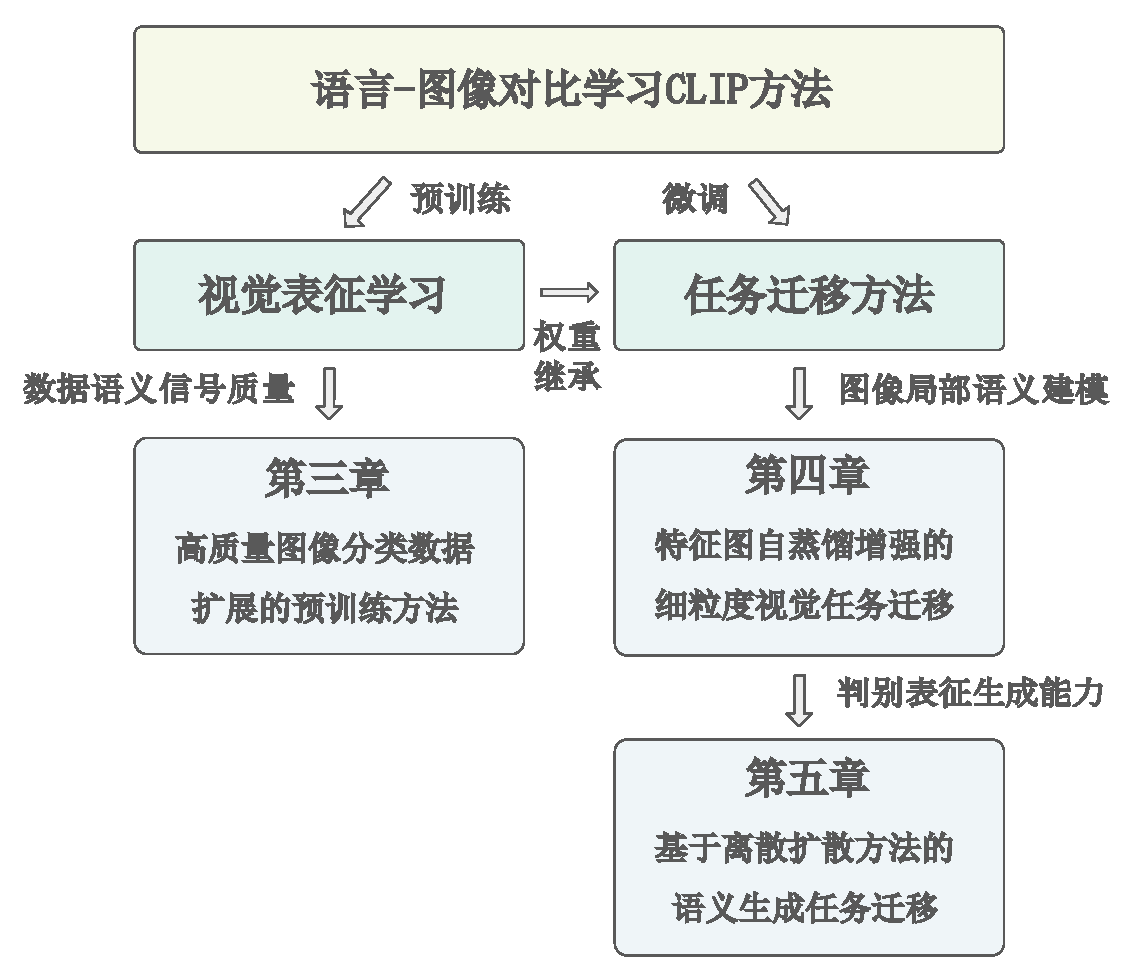
\includegraphics[width=0.9\linewidth]{figures/论文-结构安排-v2.pdf}
  \caption{本文结构安排示意图}
  \label{fig:7-thesis-structure}
\end{figure}

如图\ref{fig:7-thesis-structure}所示,本研究以基于语言-图像对比学习的视觉表征学习和迁移方法为核心,针对CLIP方法在预训练数据语义质量和下游任务适应性方面的关键挑战展开研究,提升了CLIP方法视觉表征学习效果和在细粒度视觉任务与语义生成任务上的迁移表现。主要研究内容与创新成果如下:

% 如何修改为楷体:https://www.cnblogs.com/LitBro/p/12074820.html
% 工作一:
\textit{提出基于高质量图像分类数据扩展的预训练方法。}
针对CLIP方法在预训练阶段面临的数据语义信号质量挑战,本文提出将对比学习框架扩展到更广泛的视觉标注形式,重点研究了如何有效利用高质量的图像分类数据。具体而言,通过重新设计图像分类任务的损失函数和分类器类型,本文实现了图像类别标签从封闭语义空间中的序号到语言模态可建模形式的转化,并将图像分类任务纳入对比学习框架,从而实现了对图像分类数据与互联网图文对数据的统一建模。为进一步丰富图像类别标签中的语义信息,本文引入外部专家知识库作为补充,对齐了不同数据标注的语义粒度,同时增强了语言模型的建模能力。实验表明,所提出的iCLIP方法显著提升了视觉-语言表征的对齐效果,还在零样本图文跨模态检索和开放集合图像识别等任务上取得了明显性能提升,成功构建了语义信息更为丰富的视觉表征。

% 工作二:
\textit{提出基于特征图自蒸馏增强的细粒度视觉任务迁移方法。}
% 视觉-语言多模态CLIP方法得到的视觉模型虽然蕴含了丰富的语义概念,并在对语义信息依赖较大的图像分类、图文检索任务上表现出色,但是它在一些弱语义的细粒度视觉任务的迁移表现并不惊艳,如物体检测、深度估计等任务。在这些任务上,CLIP视觉模型的迁移表现与不依赖任何语义信息的自监督方法,尤其是像素级自监督预训练方法相比并无优势。
针对CLIP模型在需要密集预测能力的细粒度视觉任务(如目标检测、语义分割、深度估计等)上迁移表现欠佳的问题,本文首先从输入完整性、训练目标粒度和损失函数设计三个维度分析了表现更优的像素级自监督方法,揭示了图像局部训练目标对细粒度视觉任务的关键作用。基于这一分析,本文提出利用知识蒸馏思想,将预训练CLIP模型的输出特征图作为教师信号,指导新初始化模型的训练。这种方法一方面无需额外数据标注即可引入细粒度视觉训练目标,另一方面能够高效继承预训练模型中的语义知识,避免了重新预训练的巨大开销。
实验表明,该特征图自蒸馏方法仅需额外3\%的计算成本,就能显著提升CLIP模型在多个细粒度视觉任务上的迁移性能。通过特征属性诊断分析发现,经过自蒸馏后的CLIP模型获得了与像素级自监督预训练模型相似的有效特性。更重要的是,这一方法具有通用性:将其应用于一个拥有三十亿参数的大规模视觉模型时,成功实现了目标检测和语义分割任务的性能突破,达到当时的最优水平。

% 工作三:
\textit{提出基于离散扩散模型的语义生成任务微调方法。} % 前面说很多方法用llm来做,比较昂贵,那这里是不就要提轻量?但我又没法和这样的模型去比较。我感觉我的工作的相关工作/context就是一坨。。时代发展确实有点快,2年没做就变天了。
尽管CLIP方法通过对比学习获得了强判别能力的视觉-语言表征,但其缺乏直接完成语义生成任务的能力。针对这一问题,本文提出了适配文本信号特性的离散扩散模型DDCap,实现CLIP模型向语义生成任务的高效迁移。具体而言,针对文本的三个关键特性——离散编码、序列长度可变和低信息冗余,DDCap方法创新性地设计了集中注意力掩码机制、长度预测模块和最佳优先推理策略。相比传统的自回归生成方法,DDCap方法具有独特优势:一方面通过同时利用前文和后文信息增强了语义生成建模能力;另一方面支持对已生成文本进行灵活修改,更适合人机交互场景。实验表明,该方法在图像描述生成任务上达到了与成熟自回归方法相当的性能水平,并在图像描述修改任务上表现更佳,验证了离散扩散模型作为语义生成任务迁移方法的巨大潜力。

% CLIP方法将视觉表征与语言表征映射到了一个共享的空间,搭建了模态之间互相转化的桥梁。一些前沿工作巧妙地利用了这一特性来完成基于文本的图像生成任务,但下游视觉-语言多模态任务中有一大类以文本为输出形式。如何利用CLIP模型解决这些基于图像的文本生成任务尚不清楚。
% 本文将针对图像生成领域主流的连续扩散模型推广为适配文本生成的离散扩散模型,首次探索了利用离散扩散模型实现基于CLIP视觉模型进行文本生成任务的可行性。
% 相比于传统自回归方法,离散扩散模型允许模型同时查看前文和后文,增强了信息利用能力;并模仿了人类的写作习惯,允许对已经生成的文本进行修改,避免了自回归方法中前向误差累计的问题,更适合一些人机交互的场景。
% 本文方法从文本信号的离散性、低冗余性和变长特性三个方面入手,有针对性地设计训练方法和推理过程,并在图像注释生成这一典型任务上证明了CLIP视觉模型与离散扩散模型组合的效果与潜力。

\section{论文的结构安排}
% 1页
% 每一章节讲了什么,需要绘图,可以把后面章节补起了之后加
% 本文的组织结构如图\ref{fig:7-thesis-structure}所示,共有6个章节。具体组织结构如下:

本文共分为6章,具体组织结构如下:

第1章是引言,介绍论文的研究课题背景与意义,详细阐述了基于语言-图像对比学习的视觉表征学习和迁移方法的研究目标、主要挑战及论文的创新贡献。

第2章是相关工作,回顾了视觉表征学习的发展历程,重点介绍语言-图像对比学习方法在预训练和微调方向的研究现状。

第3章介绍基于高质量图像分类数据扩展的CLIP预训练方法。该章节首先分析CLIP方法使用的互联网图文对数据中的噪声问题,提出将对比学习框架扩展到图像分类数据后的多数据源统一建模方法,并通过引入外部专家知识库扩充图像标签的语义信息,最后在零样本开放集合图像识别、图文跨模态检索等任务上证明了该方法的优势。

第4章介绍增强细粒度视觉任务迁移性能的特征图自蒸馏方法。该章节对比分析CLIP方法与像素级自监督方法的设计异同和迁移性能差异,提出基于特征图自蒸馏增强的细粒度视觉任务迁移方法,从而实现在没有额外数据标注的情况下引入图像局部训练信号,并通过模型特征属性诊断和多个下游任务的迁移性能提升验证了该方法的有效性和通用性。

第5章介绍基于离散扩散的语义生成任务迁移方法。该章节针对文本信号相比于图像信号的特殊性,设计适配的文本生成离散扩散框架,包括集中注意力掩码机制、长度预测模块、最佳优先推理测觉等机制,并在图像描述生成和修改任务上对该方法进行了分析。

第6章总结了论文的主要研究成果,分析目前完成工作的局限性,并探讨领域未来的研究方向。
% !TeX root = ../main.tex
\chapter{研究现状}
\label{cha:relate}
第\ref{sec:pt-related}节中首先简要回顾了传统视觉模型预训练方法,包括基于图像分类的有监督方法和基于图像自身的自监督学习的方法。随后,第\ref{sec:vl-related}节介绍了基于自然语言监督的视觉表征学习方法及其训练数据研究,并详细分析了从早期方法到语言-图像对比学习方法的发展历程。在此基础上,第\ref{sec:clip-related}节深入讨论了语言-图像对比学习在视觉表征增强以及下游任务迁移等方面的研究现状。


\section{传统视觉模型预训练方法}
\label{sec:pt-related}
% 这里是否花点章节介绍Pre-CLIP之前的一些工作?
% 总:    重提一下计算机视觉的里程碑时刻ImageNet的提出时,已经有初步的设想(WordNet)通过文本来构建信号,但因为历史原因,最终还是用无序无语义的label index的分类进行建模,使用文本的很少。CC出现是一个很强的信号(Crowd VL Data),基于此VirTex/ICMLM是两个早期探索,说一下贡献和局限性。
% Ins-Tag
% CC,LocNar(细粒度的),还有UNSUPERVISED VISION-LANGUAGE GRAMMAR INDUCTION WITH SHARED STRUCTURE MODELING等
% VirTex,ICMLM

%%% 回顾历史,尽量不要太长(0.5-1页左右)
在基于自然语言监督的视觉表征学习方法出现之前,视觉模型预训练方法主要分为三类:基于图像分类的有监督方法、基于图像话题标签的弱监督方法和基于图像自身的自监督方法。这三种方法对语义信息的利用程度各不相同,在预训练数据的可扩展性上也存在差异,形成了视觉预训练的三个发展阶段。 % 而变革的底层驱动力来自于进一步增强方法的可扩展性。

% 有监督 重提WordNet,语义变label,卡住泛化性
% 弱监督 主要提Meta的Ins-Tag,label变tag,domain狭窄
% 自监督 一次转向,抛弃任何语义信号的监督,回到视觉模型预训练本身

% 这里其实可以画个图
% 在视觉模型预训练方法研究早期,已有不少研究工作探索使用有语义的训练信号来监督视觉模型训练的方法\cite{devise},但长久以来并未找到足够高效,且可扩展性较强的方式。
视觉模型预训练方法的第一个发展阶段的里程碑是提出了ImageNet数据集\cite{deng2009imagenet}。以此为基础,基于图像分类任务的有监督预训练方法\cite{alexnet,resnet,googlenet,densenet}得到了飞速发展。
ImageNet数据集是基于词汇网络\cite{miller1995wordnet}(WordNet)构建的。词汇网络建立了各类单词与概念之间的知识图谱关系,而ImageNet数据集则从中选取部分名词概念,通过搜索引擎收集并经人工校验,为每个类别整理了相应的图片集合。
基于图像分类任务的有监督预训练方法将每类图片对应为一个类别序号,并限制模型需要识别的总类别数目。比如,常用的ImageNet-1K子集上的图像分类任务构建了1000个最常见类别集合进行图像识别训练。
这种预训练方法虽然使用了包含语义信号的训练数据,但在方法建模上并未直接使用类别标签自带的语义信息。因此,这种预训练方法在跨类别集合识别任务上的泛化效果不佳\cite{imagnettransfer},无法处理开放集合图像识别问题。此外,图像分类数据集的构造成本较高,因此常见数据集至多包含千万级别图片,可扩展性不佳。
虽然有不少工作尝试将这种基于图像分类任务的预训练方法进行大规模扩展,比如谷歌公司的JFT-300M\cite{Sun_2017_JFT300m}和JFT-3B\cite{zhai2022scaling}数据集。这些数据集促进了Transformer模型结构\cite{Transformer}在视觉领域中的应用\cite{dosovitskiy2020vit, coatnet},并推动了这类模型结构的进一步扩展\cite{zhai2022scaling, vit22b}。但由于隐私政策、商业考虑等各类原因,这些后续工作所提出的数据集和模型均未开源,相关学术成果也无法复现或使用。

为了扩展可用预训练数据来源,提升模型的泛化效果,研究者提出了弱监督预训练方法,其中代表性工作是IG-3.5B数据集\cite{mahajan2018exploring}。该数据集采用了照片墙应用(Instagram)上数十亿公开图片作为数据源,以用户添加的话题标签(Hashtag)作为图像标注。
这项工作开创性地使用了大规模标注有噪声的图像数据进行预训练,也将ImageNet数据集的单类别识别问题拓展为多类别识别问题,增加了预训练阶段的训练信号。
但与基于图像分类任务的有监督预训练方法类似,基于图像话题标签的弱监督预训练方法仍然将话题标签映射为固定集合内的类别序号,并不直接利用标注中的语义信息,因此这种方法的视觉表征语义能力较弱,跨类别集合的泛化性欠佳。
此外,这两类预训练方法都局限于固定类别集合的分类问题,因此训练信号较为稀疏。以ImageNet数据集为例,其包含了21841个不同的图像类别,每个类别序号仅能为单个图像样本提供约14比特的训练信息。在更常用的ImageNet-1K子集中,这一数值进一步缩小,只有约10比特。因此,这些预训练方法容易出现模型过拟合问题,限制了预训练模型的泛化性。

% 弱监督预训练方法拓展了视觉模型训练信号的来源。IG-3.5B数据集\cite{mahajan2018exploring}利用了脸书公司旗下的产品进行数据收集,将原先有监督预训练方法使用的单类别概念推广至任何与图像相关的话题标签(Hashtag)。另一类弱监督预训练方法则利用模型自己标注、自己训练的自举方法来增加监督信号来源\cite{yalniz2019billionscalesemisupervisedlearningimage,softteacher,mixedtraining},因此也被称为半监督训练方法。
% 但不管是利用话题标签作为标注或模型自主生成标注的方法,弱监督预训练过程中监督信号的语义信息始终有限。

为了进一步增加预训练阶段可用的训练数据,基于图像自身的自监督预训练方法放弃了难以建模和获取的语义信号,转而挖掘图像自身信息进行自我监督学习,使得预训练阶段的可用数据量在理论上可以无限扩展。
基于图像自身约束的自监督预训练方法有两个成功应用,分别是以SimCLR方法\cite{chen2020simple}为代表的对比学习预训练方法,和以MAE方法\cite{he2022masked}为代表的掩码图像模型预训练方法。前者方法利用图像的空间连续性、平移不变性等假设,要求模型识别两张数据增强后的图像是否属于同一原始图像\cite{moco,byol,dino},而后者则受自然语言处理领域发展\cite{BERT,gpt2}和Transformer模型结构在视觉领域应用\cite{dosovitskiy2020vit}的影响,强调关注图像作为二维信号的内部上下文关系,要求模型通过被掩码的部分图像恢复出完整的原始图像或特征图\cite{ImageGPT,bao2021beit,xie2022simmim,baevski2022data2vec}。
由于这些方法利用图像自身约束构造了更丰富的训练信号,比如对比学习方法的训练信息量与数据集中图像实例数目正相关,在常见数据集中为20至30比特;而掩码图像模型的训练信息量与图像分辨率正相关,通常包含$10^6$至$10^7$比特。因此,这些方法不容易出现预训练过拟合的问题,可以驱动大规模模型训练。
但是,由于自监督预训练方法在预训练过程中不使用任何语义信息,因此其依赖额外的视觉表征与语言表征的对齐阶段使得模型完成从感知特征到语义概念的映射。
此外,虽然自监督预训练方法的理论训练信号非常丰富,但由于这些训练信号侧重低级感知能力,多样性不足且不包含语义信息,因此这种预训练方法的数据利用效率并不高\cite{SEER, xie2023data},限制了此类方法的进一步扩展。

% 自监督预训练方法利用图像自身约束作为视觉模型训练信号的来源。实例级自监督方法以MoCo\cite{moco}和SimCLR\cite{chen2020simple}为代表性工作,其核心思想是将同一图像的不同视图视作对同一抽象对象的不同描述,或称为正样本对,而将不同图像的不同视图视作负样本对。MoCo\cite{moco}方法通过动态字典维护负样本对,而SimCLR\cite{chen2020simple}方法将其简化,只依赖当前批内图像作为负样本对。后续的代表性工作,如BYOL\cite{byol}和DINO\cite{dino},则使用双网络分支和特征一致性损失消除了对实例级对比方法中负样本的依赖。% 都是sg-ema+online,不对称结构,BYOL是ResNet+MSE,DINo是ViT+-plogq;https://blog.csdn.net/qq_56591814/article/details/127564330
% 另一类自监督预训练方法则是利用原始图像或特征图像素级别监督的像素级自监督方法。此类方法深受自然语言处理领域\cite{BERT,gpt2}发展和Transformer模型结构在视觉领域应用\cite{dosovitskiy2020vit}的影响。ImageGPT\cite{ImageGPT}和BEiT\cite{bao2021beit}受掩码语言建模方法\cite{BERT}启发,分别利用像素空间聚类和离散变分自编码器\cite{dVAE}的方式对图像进行标记化后进行序列掩码建模。后续的工作则进一步简化,通过回归损失消除了对图像标记化步骤的依赖。MAE和SimMIM\cite{he2022masked, xie2022simmim}方法提出通过掩码图像直接预测原始像素作为预训练的代理任务。Data2Vec\cite{baevski2022data2vec}方法则扩展了DINO\cite{dino}等双网络分支的工作,利用掩码图像的特征图一致性作为监督信号。这种方法与知识蒸馏\cite{deit,hinton2015knowledge}有相似的思想,也启发了本文第\ref{cha:fd}章的工作。

% 以vision model出发的一些历史回顾;1.2.1主要列了思想和代表性工作,这里要把更多相关工作给引入进来(1页以内)
% 这里可以仿照达哥做一个图;但主要担心是和1.2.1 写得太像。
% 有监督的imagenet,jft300m(Sun_2017_JFT300m),jft3b;scale vit(zhai2022scaling),vit22b

\section{基于自然语言监督的视觉表征学习方法}
\label{sec:vl-related}
% 视觉-语言多模态预训练方法主要分为两类。第一类方法被称为视觉-语言多模态融合方法。这类方法从已经预训练好的视觉模型和语言模型出发,通过引入额外的模型结构和代理任务对视觉表征和语言表征进行融合。
% % 并利用前文提到的互联网\{图像,替代文本\}对数据\cite{YFCC100M, sharma-etal-2018-conceptual, changpinyo2021conceptual}进行学习。
% 第二类方法被称为视觉-语言多模态联合预训练方法,包括本文的主要研究对象语言-图像对比学习预训练方法。这类方法从预训练阶段就考虑了视觉表征和语言表征的对齐与融合问题,通过视觉信息和语言信息互相监督的方式,使其天然具有处理视觉信息与语言信息的能力。
相比传统视觉模型预训练方法,基于自然语言监督的视觉表征学习方法直接利用文本描述中的丰富语义信息驱动视觉表征学习。本节将从训练数据构建和训练方法两个方面,分析这类方法的发展历程。% 特别地,我们将重点关注从早期的密集图像描述数据集,到近期的大规模图文数据集的演进过程,以及从基于文本生成的预训练方法到语言-图像对比学习方法的技术进展。

\subsection{训练数据研究}
%%% 引出基于语言监督的视觉模型训练的重要工作(0.5-1页左右)
% 分析主要目标等等
% 主要推动力:data
% \todo{图:有监督、弱监督、自监督、语言监督(vg,caption)}
% 得益于自然语言处理领域的最新进展\cite{Transformer,BERT,gpt2,elmo},视觉-语言多模态联合预训练方法登上历史舞台。站在视觉模型预训练的角度,视觉-语言多模态联合预训练方法本质上是利用语言信号为视觉模型提供监督信息。
数据驱动是“预训练-微调”范式的核心理念之一。基于自然语言监督的视觉表征学习方法的发展,与其训练数据形式的演进密不可分。
% 得益于自然语言处理领域的最新进展\cite{Transformer,BERT,gpt2,elmo},相比于第\ref{sec:pt-related}节中介绍的三种视觉模型预训练办法。
% 视觉-语言多模态预训练方法的核心是对数据中的语义信息进行充分挖掘和建模,其本质是用语言信号驱动视觉模型训练。
% 相比于使用图像类别序号作为训练信号的有监督方法和弱监督方法,视觉-语言多模态预训练方法可利用的语义信息内容更加丰富、形式更加多样、描述粒度更全面。

% 将视觉模型的监督信号从用类别序号表示的名词概念或者话题标签,推广到内容多样更强、描述粒度更细的自然语言信号。
% 因此此类方法在直接利用语义信息作为监督的同时,提升了监督信号的泛化性和所蕴含的信息量。
Visual Genome\cite{krishna2017visual}是基于自然语言监督的视觉预训练数据构建方法的重要代表。该方法提出稠密图像标注的概念,为每张图像标注了对象信息、属性特征、位置信息和相对关系等各类内容,并将这些信息用自然语言表示作为预训练信号。这种方法也启发了后续的稠密图像描述任务和多模态大模型与人类意图对齐任务\cite{imageinwords,flexcap,densecap}。
但这类方法的训练信号建模复杂,标注成本高,限制了训练数据样本的可扩展性,不适合作为大规模预训练数据构造方法。
因此,数据获取更容易、可扩展性更好的互联网图文数据对构建方法\cite{YFCC100M, sharma-etal-2018-conceptual, changpinyo2021conceptual}逐步替代了基于稠密图像标注的数据构造方法。
互联网图文数据对构建方法创新地利用网页代码中描述图像内容的文本属性,来构建视觉信息与语言信息配对的训练数据。得益于互联网技术的普及和用户生成内容的广泛应用,这类图文数据对通常具有千万甚至亿级规模,具有获取成本低、数据多样性好的优势。
虽然互联网图文数据对不如稠密图像标注数据的语义信息含量高,同时受数据噪声干扰较大,但由于其出色的数据可扩展性,使得这类数据构造方法已经成为主流的训练数据获取方法,为后续相关工作的发展奠定了基础。

然而,互联网图文数据对构建方法也面临两个主要挑战:首先,互联网数据缺乏质量控制和规范标准,存在大量噪声数据;其次,开源的图文数据集规模较小,限制了相关研究的进一步开展。
为解决这些问题,研究界在提升预训练数据质量和开源更大规模数据集等方面提出了诸多工作。
YFCC\cite{YFCC100M}和Conceptual Captions系列\cite{sharma-etal-2018-conceptual,changpinyo2021conceptual}工作率先开源了较大规模的互联网图文数据对,并提出通过图像分辨率和长宽比、文本长度和规范度等多维度人工规则来过滤低质量数据。但这类早期数据集的规模通常仅有千万级别,难以满足大规模预训练的需求。
由于互联网开源项目Common Crawl\cite{cc}提供了海量网页数据资源,因此LAION等工作\cite{schuhmann2021laion400m,schuhmann2022laion5bopenlargescaledataset,COYO-700m}从中构建并开源了更大规模的数据集,将规模从亿级扩展到十亿级,并创新地利用预训练好的语言-图像对比学习模型来评估和筛选高质量的图文数据对。DataComp工作\cite{datacomp}则基于LAION的开源数据集,构建了对比数据质量筛选方式优劣的评测基准。
MetaCLIP\cite{xu2024demystifying}工作则从更深层次探讨了数据质量问题。该工作遵循OpenAI CLIP工作\cite{radford2021learning}的数据构建方法,从文本N元语法分布的角度优化概念的多样性和均衡性,有效提升了数据集中独特语义信息的覆盖率。
此外,一些研究开始探索新的数据组织形式。MM-C4\cite{MM-C4}和OBELICS\cite{OBELICS}等工作提出了多图像多文本的交错图文对形式,以期通过更复杂的对应关系提供更丰富的语义信息。

% (Alternative Text,简称为Alt-Text)作为低成本、富语义、高多样性的自然语言监督信号,驱动视觉模型预训练。
% 替代文本本身是一种在网页代码中用于描述图像内容的文本属性。当图像无法显示时,浏览器会显示这些替代文本。因此这些替代文本常被用于帮助视觉失能用户理解图像内容,或被搜索引擎用于优化图文检索系统。
% 这类语义信号虽然不如Visual Genome方法所标注的内容信息含量高,也存在大量噪声问题。但由于互联网多年发展的积累,这类文本往往以千万甚至亿级别的规模存在,而且与图像成对出现,形成天然的\{数据,标注\}配对。


\subsection{训练方法研究} %{视觉-语言多模态模型模态对齐训练方法}
% \subsection{视觉-语言多模态联合预训练方法} %\paragraph{视觉-语言多模态模型联合预训练方法}
% % 先介绍一点VirTex相关的
% % 再介绍CLIP
% % 再介绍CLIP++
% 与视觉-语言多模态融合方法不同,视觉-语言多模态联合预训练方法不依赖单模态预训练的视觉模型和语言模型,相反地,这类方法从预训练阶段就通过视觉信息和语言信息互相监督训练的方式,实现了不同模态表征的融合,无需额外的模态表征融合阶段。
基于自然语言监督的视觉表征学习方法的核心是对数据中的语义信息进行充分挖掘和利用,从而驱动视觉模型训练。
% 相比于使用图像类别序号作为训练信号的有监督方法和弱监督方法,视觉-语言多模态预训练方法可利用的语义信息内容更加丰富、形式更加多样、描述粒度更全面。

如第\ref{sec:clip-introduce}节中所述,早期基于自然语言监督的视觉表征学习方法主要受自然语言处理领域启发:以图像为条件的掩码语言模型\cite{sariyildiz2020learning}继承了掩码语言模型\cite{BERT}(BERT)的掩码预测思想,而从文本标注中学习视觉表征方法\cite{desai2021virtex}则采用了生成式语言模型\cite{gpt2}(GPT)的自回归设计。
受限于较低的掩码比例,掩码语言模型的训练信号较为稀疏,训练效率不高。相比之下,生成式语言模型的自回归设计基于马尔可夫性质,将文本序列的联合概率分解为单文本标记预测的条件概率乘积,能够充分利用完整的语言信息。这种方法在训练单文本标记预测任务时都依赖正确的前序文本(即“教师强制”策略),因此训练效率更高。
然而,尝试将从文本标注中学习视觉表征方法扩展到更大规模时,研究者遇到了重要挑战:这类方法假设图像与文本存在严格对应关系,这与互联网图文数据对中普遍存在的噪声特性不相符。
为解决这一问题,研究者提出了两种改进方案:前缀语言模型\cite{SimVLM}(PrefixLM)和序列到序列模型\cite{GIT}(Seq2Seq)。这些变体将部分文本内容从训练目标转换为输入条件,放松了图像与文本强对应约束,从而在训练效率和数据可扩展性之间取得了更好的平衡。为了进一步放宽图像与文本严格匹配的数据假设,研究者开始探索另一种范式,即语言-图像对比学习方法,来优化视觉与语言表征间的相对关系。

% 此外,这些方法比较适合迁移到依赖多模态表征融合的下游任务,但在单模态下游任务上的微调表现欠佳。

% 以图像为条件的掩码语言模型\cite{sariyildiz2020learning}是早期代表性的视觉-语言多模态预训练方法。这种方法是自然语言处理领域中的掩码语言模型\cite{BERT}的扩展。具体而言,给定一条配对的图像与文本数据,该方法首先随机选择一定比例的文字用一个特殊的掩码词元进行替换,其次要求模型利用图像信息,预测被替换的文字的原始内容。
% 这里将可训练模型参数记为$\theta$,将图像信息记作$I$,并将长度为$n$的文本序列记作$T=\{t_1,\cdots ,t_n\}$。以图像为条件的掩码语言模型预训练方法在最大化如下概率估计:
% \begin{equation}
%     \max_{\theta}\sum_{t_i\in T'}\log\left({p_{\theta}(t_i|T-T',I)}\right),  
%     \label{eq:icmlm}
% \end{equation}
% 其中$T'$为被替换成掩码词元的部分文字集合,$T-T'$表示文本序列中未被替换成掩码词元的文字集合。这种视觉-语言多模态预训练方法和掩码语言模型类似,只会对长度为$n$的文本序列进行部分掩码训练。通常的掩码比例为15\%。因此针对每条图文对训练数据,该方法只能借助其中一小部分语义信息来驱动模型训练。

% 从文本标注中学习视觉表征方法\cite{desai2021virtex}的出现正是为了在模型预训练过程中尽可能利用更多的语义信息进行学习。这种方法同样受自然语言处理领域的发展启发,是自回归语言模型\cite{gpt2}在视觉-语言多模态预训练方向的扩展。
% 与以图像为条件的掩码语言模型方法不同,从文本标注中学习视觉表征方法要求模型利用图像信息,预测对应文本的完整文字序列。虽然从理论上而言,将以图像为条件的掩码语言模型方法中的掩码比例设置为100\%,即可驱动模型去预测完整文字序列,但这个预训练任务难度过高,几乎无法提供有意义的学习方向。
% 为解决这一问题,从文本标注中学习视觉表征方法借鉴了自回归语言模型中的马尔可夫性思想。将文本从左往右的书写顺序理解为系统的前后状态,而马尔可夫性质决定了系统的下一状态只依赖于当前状态,因此,文本序列的生成过程可以被拆分为从左往右的迭代过程。
% 与式\eqref{eq:icmlm}中符号一致,从文本标注中学习视觉表征方法在最大化如下概率估计:
% \begin{equation}
%     \max_{\theta}\sum_{i=1}^{n}\log\left({p_{\theta}(t_i|t_{1:i-1},I)}\right)    
%     = \max_{\theta}\log\left({p_{\theta}(t_{1:n}|I)}\right),
%     \label{eq:character-level}
% \end{equation}
% 其中$t_{1:0}$可以理解为空序列。可以看出,从文本标注中学习视觉表征方法通过马尔可夫性,将基于图像信息的文本序列预测任务拆分成了多个单文字预测任务,并在每个单文字预测任务中都基于正确的前序文本序列进行预测。这种思想也被称为“教师强制”(Teacher Forcing)。
% % https://www.cnblogs.com/dangui/p/14690919.html
% 通过这种方式,从文本标注中学习视觉表征方法可以充分利用每条图文对训练数据中的语义信息进行模型预训练,进一步增强了模型对语义信息的建模能力。相比于以图像为条件的掩码语言模型预训练方法,这种方法得到的视觉模型在各类下游任务上的迁移效果更佳。

% 早期视觉-语言多模态模型联合预训练方法主要是扩展了掩码语言标记建模BERT模型\cite{BERT}和基于自回归语言建模的GPT模型\cite{gpt2}。
% 前者以ICMLM方法\cite{sariyildiz2020learning}为代表。这种方法利用\{图像,文本\}配对数据完成基于图像内容的掩码语言标记建模。通常而言,每一条输入文本的15\%的词会被随机掩码。因为文本内容的冗余性比较低,信号具有离散性,因此掩码标记无法提供除占位信息之外的任何内容。这一点也在第\ref{chap:ddcap}章所讨论。这一特点导致掩码比例无法被扩展到一个较大的值\cite{BERT, BERTmask}。
% 有限的掩码比例导致这类方法的单样本训练信号较少,学习效率并不高,后续逐渐被以VirTex\cite{desai2021virtex}为代表的基于自回归语言建模的工作所取代。基于自回归的方法建模了整条样本的联合概率分布,训练信号丰富,是大规模扩展工作的主要思路\cite{SimVLM, GIT},并延伸出前缀语言模型\cite{SimVLM}和序列到序列模型\cite{GIT}两种变体。
% 但这些后续工作以完成视觉-语言多模态下游任务为主,未讨论过其视觉模型的迁移效果,也无法将其用于大规模图文检索系统。
% 此外,如节\ref{sec:instance-purpose}中的分析,此类方法建模了图像与文本的强对应关系,对数据质量要求较高,这也是GiT\cite{GIT}方法仅用一半数据就超过SimVLM\cite{SimVLM}方法的重要原因之一。


\begin{figure}
  \centering
  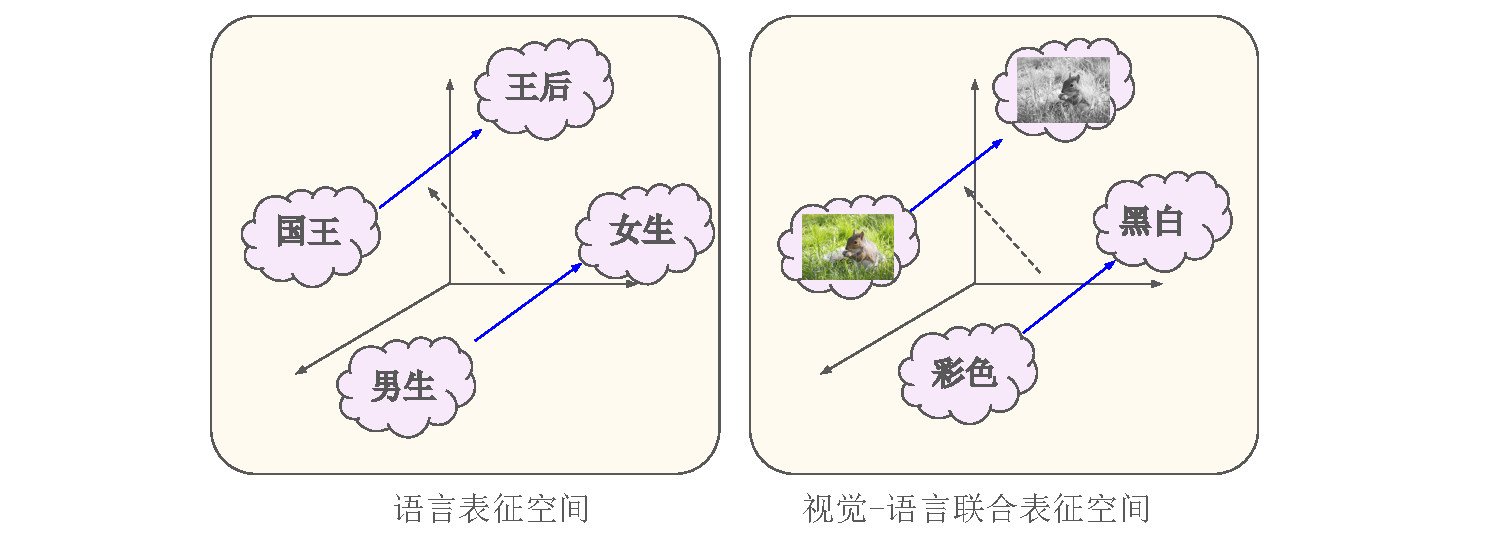
\includegraphics[width=1.0\linewidth]{figures/论文-CLIP性质-v2.pdf}
  \caption{语言表征空间与视觉-语言联合表征空间的相似性示意图}
  \label{fig:clip-word2vec}
\end{figure}

语言-图像对比学习(CLIP)方法\cite{radford2021learning,jia2021scaling,pham2023combined}借鉴了实例级对比学习自监督方法的思想,将视觉表征的预训练任务从“预测语言信息”转变为“与语言表征对齐”。这种多模态对比学习策略通过建模不同模态表征间的相对距离,有效降低了对图像与文本严格对应关系的依赖。同时通过构建视觉-语言联合表征空间,CLIP方法能够驱动模型学习更具判别性的表征,从而提升了模型在下游视觉任务上的迁移效果。
更重要的是,CLIP方法构建的视觉-语言联合表征空间具有独特的性质,使得CLIP方法特别适合用于模态表征提取和跨模态表征转换与检索等任务。
视觉-语言联合表征空间的性质与语言表征空间\cite{word2vec,distword2vec}有相似之处。如图\ref{fig:clip-word2vec}左侧所示,在语言表征空间中,不同概念的表征之间存在可解释的线性关系。例如,“女生”的表征减去“男生”的表征,再加上“国王”的表征,可以得到“王后”对应的表征。
CLIP方法构建的联合表征空间也展现出类似的线性关系。如图\ref{fig:clip-word2vec}右侧所示,通过“黑白”语言表征减去“彩色”语言表征,可以获得表示颜色变换的向量,再将这个向量应用到彩色图片的视觉表征上,就能有效检索到对应黑白图像的视觉表征。
这种多模态表征对齐能力不仅使得CLIP方法在图文跨模态检索任务上表现优异,还表明CLIP方法习得的视觉表征中包含了丰富的语义信息,为开放集合图像识别任务的发展提供了重要基础。

% 将自监督预训练方法\cite{moco, chen2020simple}的正负样本对思想引入视觉-语言多模态训练中。
% 视觉模型自监督预训练工作本质上将同一图像的不同视图视为对某一抽象对象的不同描述。自监督对比学习的核心思想正是建模关于此抽象对象的不变表征。
% 将这一思想推广到\{图像,文本\}配对数据后,CLIP方法将图像和文本分别理解为某一抽象对象的不同描述,因此配对的图像和文本可以被视作正样本对,而任一不配对的图像与文本均被视作负样本对。% 这写的不是车轱辘话?

\section{语言-图像对比学习方法}
\label{sec:clip-related}
作为一种重要的“预训练-微调”方法,CLIP方法的相关研究主要关注如何提升预训练阶段的可扩展性,增强其视觉表征的语义建模能力,同时提升CLIP方法在多种下游任务中迁移表现和泛化性。

\subsection{视觉表征学习增强方法研究}
% 泛化能力\cite{ftclip2021, clip-generalize, languagehelpvision, clipshortcut}
% 预训练效果\cite{li2022supervision,TCL,SLIP,MaskCLIP,CoCa,EVA,pham2023combined,pali,LiMoE,palix}
% 可以recall 目标
% 如前文所述,预训练阶段是整个“预训练-微调”范式的核心。因此如何进一步提高语言-图像对比学习方法的预训练可扩展性,增强视觉表征与语言表征的对齐效果是重要研究目标之一。各类工作围绕如何高效扩展预训练数据和模型参数规模,以及如何进一步增加预训练信号的来源,降低预训练数据噪声干扰展开了系列研究。
预训练阶段是整个“预训练-微调”范式的核心。因此,进一步扩展CLIP方法、增强其视觉表征的语义建模能力、提高视觉表征与语言表征的对齐效果,是该领域的重要研究方向。现有工作主要围绕扩展预训练数据和模型规模、降低预训练成本与代价、拓宽预训练信号来源以及分析模型特征属性展开。

\paragraph{扩展预训练数据与模型规模} 由于CLIP方法具备大规模扩展的潜力,因此许多研究致力于进一步提升其可扩展性。
BASIC方法\cite{pham2023combined}从工程优化角度,提升了CLIP方法的可用数据规模、模型参数数量和训练批次大小。相比于最初的OpenAI CLIP方法\cite{radford2021learning},BASIC方法采用的训练数据规模扩大了16倍,视觉模型参数增加了4倍,训练批次大小增大了4倍,充分展示了CLIP方法的可扩展性。
PaLI系列方法\cite{pali,palix}不仅进一步提升了视觉模型的参数规模,还结合大语言模型提升了CLIP方法对语言信息的建模能力。此外,PaLI方法将以英文为主的互联网图文数据对扩展至覆盖100多种语言的图文数据对,显著增强了CLIP方法在跨语言任务上的泛化能力。
LiMoE方法\cite{LiMoE}引入混合专家\cite{gshard}(Mixture of Experts)模型结构,分别为视觉模态和语言模态设计独立的专家模型。在显著提升CLIP方法模型参数规模的同时,LiMoE方法通过部分参数激活的方式降低了计算成本,使得训练更加高效。

% 引入知识蒸馏方法
\paragraph{构建高效轻量的CLIP方法}
% 虽然这些方法在增强CLIP方法的预训练效果上取得了印象深刻的表现,但这些大规模的数据和模型一方面并未开源以推动研究进展。
随着CLIP方法预训练规模的不断扩大,其对大规模计算资源的依赖日益增加。高昂的训练成本限制了许多研究机构开展相关工作,因此提高预训练效率,降低预训练成本成为重要研究方向。CLIPA系列方法\cite{CLIPA,CLIPA-v2}提出了“逆扩展定律”:训练的模型参数量越大,所需的输入图像分辨率和文本序列长度越小,因此这一发现有助于降低预训练的计算开销。A-CLIP系列方法\cite{ACLIP,FLIP}则借鉴了自监督方法中的掩码图像模型思想,对输入图像进行部分掩码来减少训练过程中的计算开销。
此外,MobileCLIP\cite{MobileCLIP}和TinyCLIP\cite{TinyCLIP}等工作采用知识蒸馏方法\cite{hinton2015knowledge}来构建小规模模型,降低了CLIP方法在应用中的成本。

知识蒸馏方法\cite{hinton2015knowledge,kim2018paraphrasing}最早被应用于卷积神经网络中,后来被成功推广到Transformer模型结构\cite{deit,wang2020minilm}。这种方法的核心在于将教师模型的知识迁移到更小的学生模型中,因此,知识蒸馏是一种常用的模型压缩手段。研究表明,在图像分类任务中,当学生模型模仿教师模型的未归一化输出时,教师模型能够提供简单类别信息之外的“暗知识”\cite{furlanello2018born},从而提升学生模型的性能。% https://blog.csdn.net/Artistzq/article/details/125372542
除了在图像分类任务得以应用之外,知识蒸馏方法在深度强化学习\cite{chaudhry2018riemannian}、终身学习\cite{zhai2019lifelong}和推荐系统\cite{chen2018adversarial}等领域都取得了显著成果。
% 训练效率\cite{CLIPA,CLIPA-v2,MobileCLIP,VisionZIP,ACLIP,FLIP}

% 这个倒是可以画个图清楚一点
\paragraph{拓宽预训练信号来源与利用方式} 
除了通过扩大规模来改进CLIP方法,研究者还探索了在CLIP方法中引入其他训练信号的方式,以提高视觉表征的学习效果。
SLIP方法\cite{SLIP}借鉴了实例级自监督方法的思想,将CLIP方法与图像自监督对比学习方法\cite{chen2020simple}结合,增强了视觉表征的建模能力。DeCLIP方法\cite{li2022supervision}则在此基础上,进一步引入掩码语言模型来提升CLIP方法的语言建模能力,并通过图像增强和文本改写等技术构造更丰富的图文对齐数据。
受视觉-语言多模态训练方法\cite{visualbert}启发,TCL方法\cite{TCL}设计了多模态表征深度融合模块,通过图文配对预测任务来加强模态间的对齐效果。该任务在形式上与掩码语言模型的下一句子预测任务\cite{BERT}一致,加强了模型对图文关系的理解。MaskCLIP方法\cite{he2022masked}则结合了像素级自监督方法,在CLIP方法中引入掩码图像模型的训练任务\cite{he2022masked},从而进一步提升视觉模型对图像结构的感知能力。
CoCa方法\cite{CoCa}则在CLIP方法中重新加入从文本标注中学习视觉表征方法\cite{desai2021virtex},要求模型在对齐视觉表征和语言表征的同时,完成基于视觉表征预测输入文本内容的训练任务。最新提出的SigLIP-2方法\cite{siglip-2}更是整合了各类视觉和语言模型的自监督方法,以实现更好的单模态表征建模能力与跨模态表征对齐效果。

% 参考FD
\paragraph{模型特征属性诊断工具} 深度学习模型由于其高维和非线性特性,因此往往被视为“黑箱”系统。为了更好地理解模型的内部机制,模型特征属性诊断工具发挥着关键作用\cite{yosinski2014transferable}。这类研究不仅有助于解释模型的决策过程,也为模型设计和优化提供了重要指导。自Transformer模型结构提出以来,众多研究工作\cite{zhou2021deepvit, dosovitskiy2020vit, goh2021multimodal, dai-etal-2022-knowledge, imagnettransfer, raghu2021vision}致力于揭示其自注意力层和前馈层的工作原理。这些研究主要从以下几个方面展开:1)通过注意力机制分析方法\cite{zhou2021deepvit, dosovitskiy2020vit}可视化注意力权重分布,反映模型如何关注不同位置的输入,揭示模型的视觉感知偏好;2)通过损失景观可视化方法\cite{li2018visualizing}分析损失函数在模型参数空间中的分布特征,理解模型训练过程中的优化轨迹和收敛特性;3)通过层间相似度分析\cite{kornblith2019similarity}考察不同模型层表征间的相似程度,探究模型的层间结构化性质;4)通过知识神经元分析\cite{dai-etal-2022-knowledge, goh2021multimodal}识别模型中对特定概念异常敏感的神经元,揭示模型内部的知识表示方式。

现有工作在扩展预训练信号来源时,通常需要维护多个模型实例\cite{TCL,MaskCLIP}或处理多个图像增强视图\cite{SLIP,TCL,li2022supervision}。这种做法显著增加了预训练阶段的计算资源消耗。同时,现有的数据语义信号质量提升方法也存在局限性。基于启发式规则的筛选方法\cite{sharma-etal-2018-conceptual}可能误判数据质量,而依赖预训练模型打分的方法\cite{schuhmann2021laion400m}对细微质量差异的区分能力有限。
针对这些问题,本文第\ref{cha:iclip}章中提出了另一种研究方法,通过对比学习思想有效整合和深度利用了人工标注的图像分类数据源。这种方法不需要增强额外的模型参数或处理多个图像增强视图,利用高质量的图像分类数据提升了CLIP方法训练数据的整体质量,增强了CLIP方法的视觉表征学习效果。

% 第一点如何获取高质量图文的数据,并增加预训练信号来源是CLIP方法进一步扩展的关键因素。很多现有数据扩展工作并不开源,而数据收集的成本比较高,而且过滤方法需要人工规则,容易存在遗漏的情况,因此本文的第一项工作,就是基于低噪声图像分类数据增强的CLIP预训练方法。通过这种方法来加强视觉表征与语言表征的对齐,增强CLIP方法零样本图文跨模态检索和开放集合图像识别能力。
\subsection{下游任务迁移方式研究}
% 可以recall 目标
% 作为一种预训练方法,除了提升预训练阶段多模态表征对齐效果,提高语言-图像对比学习方法在各类下游任务上的迁移表现,并泛化到尽可能多的下游任务也是一个重要的研究目标。
作为一种预训练方法,CLIP方法的价值不仅体现在多模态表征的对齐效果上,更重要的是其迁移到下游任务后解决实际任务的能力。因此,提升CLIP方法在不同类型任务上的迁移性能并扩展其应用范围,也是该领域的重要研究方向。现有工作主要围绕开放集合识别的视觉任务、多模态语义生成任务以及多模态图像生成任务展开。

\paragraph{开放集合识别的视觉任务迁移}
% 迁移部分可以多加一些clip for zs seg/det这种工作
CLIP方法在零样本开放集合图像识别任务上展现出优异性能,这促使研究者探索将其开放集合识别能力迁移到更广泛的视觉任务中。
在目标检测任务中,ViLD\cite{ViLD}和F-VLM\cite{F-VLM}等方法将目标检测任务分解为定位和识别两个阶段,成功实现基于CLIP方法的开放集合目标检测任务迁移。这一思路启发了后续一系列工作\cite{Zhong_2022_CVPR, glip, detclip, detclip-2, detclip-3}。这些工作通过构建更细粒度的单词-区域对比学习方法,实现了真正意义上的开放集合目标检测能力。
在语义分割任务中,研究者致力于提取CLIP方法蕴含的像素级语义信息。相关工作\cite{denseclip, zsseg, openseg}主要采用两种策略:第一种策略是参考开放集合目标检测任务做法,将语义分割任务拆分为物体掩码预测和语义识别两个阶段;第二种策略是利用CLIP方法的视觉模型中的自注意力机制,聚合并提取属于同一类别的像素位置和语义信息。
此外,在少样本图像识别任务中,CoOp等工作\cite{coop,cocoop}通过引入提示微调等技术,显著提升了CLIP方法在精细类别图像识别任务上的迁移表现。
% 还有few-shot transfer的工作。

% 这个detclip竟然也讨论了dictionary enhancement的概念 for openvocabulary的det啊哈哈哈

\paragraph{多模态语义生成任务迁移}
% 图生文CLipCap;% 可以包括一些图像描述任务的讨论,以及之前放在2.2.2. 的视觉-语言多模态融合方法
% 还有后续的clip+llm的工作也可以写进来
% 语言-图像对比学习方法在预训练过程中允许模型同时理解视觉信息与语言信息,因此也非常适合迁移到多模态下游任务中。
% 视觉-语言多模态融合方法\cite{visualbert, vl-bert, uniter, OSCAR, VinVL, LEMON}本质上是一种两阶段的预训练方法。这类方法从已经预训练好的视觉模型和语言模型出发,通过引入额外的模型结构和代理任务对视觉表征和语言表征进行融合,再将得到的视觉-语言多模态模型迁移到各类下游任务中。
% 受掩码语言模型\cite{BERT}启发,这类方法往往把基于图像的掩码语言模型作为主要代理任务,并利用多模态数据特有性质来构建辅助代理任务,从而驱动视觉表征和语言表征融合。
多模态语义生成任务涵盖多个重要方向,包括图像描述生成\cite{vinyals2015show,karpathy2015deep}、视觉问答\cite{vqa}以及近期兴起的复杂人类指令理解任务\cite{llava}。其中,图像描述生成作为最基础的多模态语义生成任务,长期以来受到广泛关注。
早期的图像描述生成方法\cite{vinyals2015show,karpathy2015deep}采用卷积神经网络提取视觉特征,配合循环神经网络作为解码器生成图像描述。后期工作引入注意力机制提升了视觉和语言信息的融合效果\cite{huang2019attention,lu2017knowing}。为进一步提高图像描述生成任务效果,一些工作探索了利用语义属性\cite{yao2017boosting}和场景图\cite{yang2019auto}等额外信息的方法。受掩码语言模型的启发,研究者还尝试了非自回归方法\cite{gao2019masked}的图像描述生成迁移方法。这些技术进展不仅推动了图像描述生成任务的发展,也为其他多模态语义生成任务提供了重要借鉴。

早期的多模态语义生成任务迁移研究\cite{visualbert, vl-bert, uniter, OSCAR, VinVL, LEMON}主要基于单模态预训练的视觉模型和语言模型展开。这些方法通过引入额外的模型结构和多模态对齐任务,实现视觉和语言表征的深度融合。这类方法的典型做法是使用在Visual Genome数据集上微调的目标检测模型\cite{butd}作为视觉表征提取器,并将其提取的各区域特征输入到掩码语言模型中,完成以图像为条件的掩码建模任务。不同方法提出了多种创新性的辅助任务来增强模态融合效果。
% 早期多模态任务迁移方法从已经预训练好的视觉模型和语言模型出发,通过引入额外的模型结构和代理任务对视觉表征和语言表征进行融合从而迁移语义生成多模态任务中。这些方法通常使用在Visual Genome数据集上微调得到的目标检测模型\cite{butd}作为视觉特征提取器,再将其输入到掩码语言模型\cite{BERT}中,完成以图像为条件的掩码建模任务。不同方法引入了额外的辅助代理任务以增强模态融合的效果。
% VisualBERT方法\cite{visualbert}参考BERT\cite{BERT}方法中的下一句子预测任务,引入图文配对预测任务以增强实例级对应关系学习。VL-BERT方法\cite{vl-bert}为保留预训练语言模型的语言建模能力,避免预训练知识的灾难性问题\cite{catastrophic},在图文数据对之外加入纯文本数据进行补充。UNITER方法\cite{uniter}则参考文本的掩码建模任务形式,对物体检测框序列构造掩码区域特征建模任务,以增强视觉表征与语言表征的融合效果。Oscar方法\cite{OSCAR}除了将物体检测框对应的区域特征和区域位置输入语言模型之外,还将每个检测框的类别信息作为额外的输入信息,提供辅助融合信号。
由于目标检测模型作为视觉表征提取器存在两个主要问题:计算开销较大且检测框采样操作影响梯度回传,因此后续研究\cite{pixelbert, soho, vilt}提出了更高效的方案:直接使用视觉模型的特征图,或采用随机初始化的块嵌入层(Patch Embedding)作为视觉表征。这些改进为多模态语义生成任务迁移的端到端优化提供了可能性。
% 目标检测模型作为视觉表征提取器非常耗时,一些后续工作\cite{pixelbert, soho, vilt}提出使用视觉模型特征图或一个随机初始化的图像块投影层作为视觉表征输入到语言模型中,为端到端优化提供可能。

CLIP方法在预训练过程中实现对视觉和语言信息的双重理解,为多模态语义生成任务迁移提供了良好基础。一些工作\cite{song-etal-2022-clip, shen2022how}讨论了如何基于早期方法\cite{pixelbert}将CLIP方法的视觉模型迁移到视觉问答、视觉蕴含等多模态语义生成任务中。而CLIPScore方法\cite{CLIPScore}则创新地利用了CLIP方法多模态表征的对齐特性,构建了一个不依赖参考文本的图像描述生成质量评价指标。
近期,随着大语言模型的快速发展,多模态语义生成任务迁移研究出现了新的趋势。以BLIP-2\cite{blip-2}为代表的一系列工作\cite{minigpt4,llava,llavanextinterleave}探索了将预训练好的大语言模型与CLIP方法的视觉模型相结合的方法,充分利用了大语言模型的语义表达能力,开创了CLIP方法在多模态语义生成任务迁移的新方式。


\paragraph{多模态图像生成任务迁移}
CLIP方法对齐了视觉表征和语言表征,为多模态图像生成任务迁移提供了新的可能。其中,Dall-E 2方法\cite{dall-e2}开创性地利用了这种对齐特性实现CLIP方法在多模态图像生成任务上的迁移:该方法首先利用CLIP方法的语言模型得到输入文本的语言表征,然后训练一个基于扩散模型\cite{ddpm,ddim}的先验模型预测对应的CLIP视觉表征,最后再通过另一个扩散模型将CLIP视觉表征转化为实际图像。Dall-E 2方法在基于文本的图像生成任务中效果出色,在大量应用中得到应用。
作为Dall-E 2方法中的关键技术,扩散模型主要分为连续扩散模型和离散扩散模型两类。连续扩散模型\cite{beatsgan,ddpm,ddim,latentdiff}对连续的输入空间或特征空间进行建模,在基于文本的图像生成领域取得了显著成果,已发展成为主流技术路线。连续扩散模型的代表性工作包括GLIDE\cite{glide}、Imagen\cite{imagen}和Stable Diffusion\cite{latentdiff}等,在图像生成质量和可控性方面展现出优异表现。
相比之下,离散扩散模型的研究相对较少。ImageBART\cite{Imagebart}和VQ-Diffusion\cite{VQ-diffusion}等工作探索了在VQ-VAE\cite{dVAE,vqvae}方法构建的图像离散代码空间中应用扩散模型的可行性,为多模态图像生成任务迁移提供了新的解决思路。
% 对于文本生成,离散扩散仅在相对玩具的问题上显示出一些初步的成功 [3,26]。最近的工作 [41] 也尝试使用连续扩散进行文本生成,但更多的是用于细粒度的控制任务。

现有研究主要关注CLIP方法在对语义依赖程度较高的开放集合识别任务上的迁移应用,而对于需要密集感知能力的视觉任务的迁移方法研究较少。针对这一问题,本文第\ref{cha:fd}章提出了特征图自蒸馏方法。该方法无需重新预训练或额外数据标注,通过引入像素级视觉训练目标,显著提升了CLIP方法在细粒度视觉任务上的迁移性能。
在多模态语义生成任务方面,现有方法通常结合大语言模型并需要复杂的表征融合实现任务迁移,训练成本和系统复杂度都很高。为解决这一问题,本文第\ref{chap:ddcap}章探索了一种基于离散扩散模型的语义生成任务迁移方法,同时探讨了扩散模型在文本生成任务中的应用前景。
%%%%%%%%%%%%%%%%%%%%%%%%%%%%%%%%%%%%%%%%%%%%%%%%%%%%%%%%%%%%


% 达哥在讨论像素级任务的研究动机时起其实分析了实例级任务的缺陷(这部分可能会在我的前一部分讨论,前一部分讨论语言监督+基于掩码和自回归的两种细粒度办法;)
% 问题:什么时候提细粒度 data(以locnar为代表的)
% 先比较重要的两个工作:VirTex,ICMLM
% 分析贡献,讲述缺陷(数据获取难度,最大监督信号信噪比)
% 引出CLIP:介绍CLIP的具体做法,将其对比纯图像的实例级方法
% 针对之前讨论的非实例级的办法的缺陷,引出为什么这个办法好(合计1-1.5页左右)
% \begin{figure}
%   \centering
%   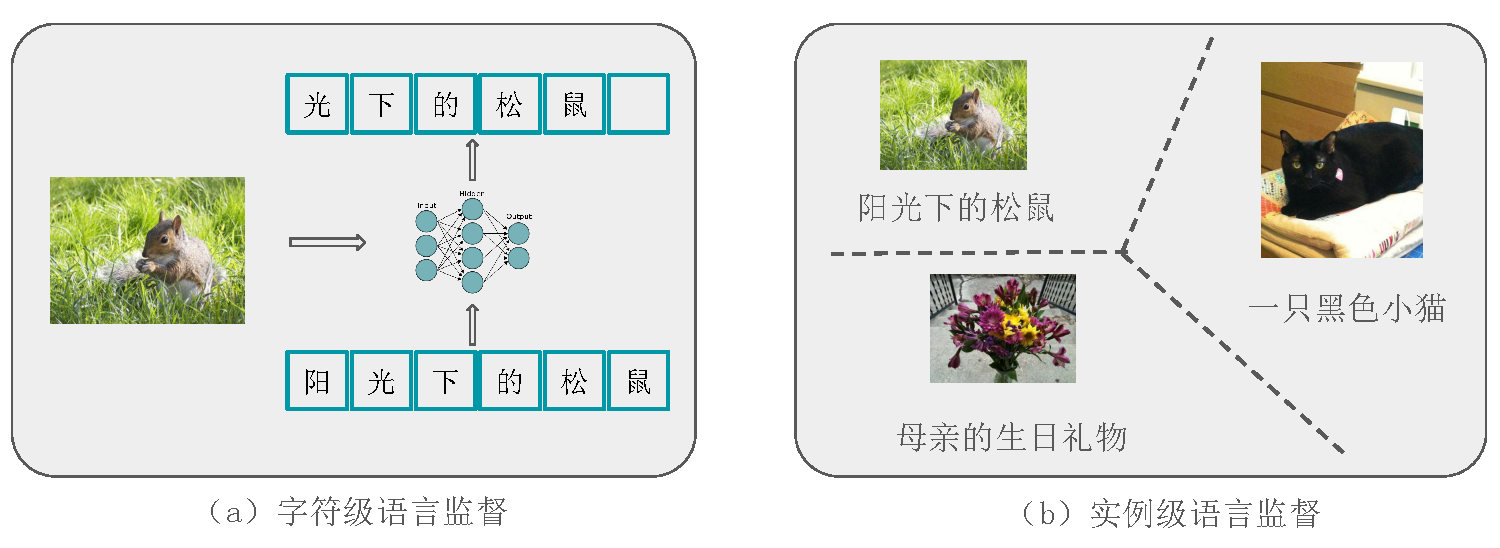
\includegraphics[width=1.0\linewidth]{figures/论文-图5-字符级-实例级.pdf}
%   \caption{字符级联合预训练方法和实例级联合预训练方法示意图}
%   \label{fig:5-character-instance}
% \end{figure}
% 如节\ref{sec:language-supervised}所述,站在视觉模型预训练的角度,视觉-语言多模态联合预训练方法本质是一种基于自然语言监督的视觉预训练方法。
% 与自监督视觉预训练方法的发展类似,基于自然语言监督的视觉预训练方法也有实例级别训练方法和更细粒度的字符级训练方法。但和自监督方法的发展历程有所区别,在实例级语言监督的方法出现之前,细粒度字符级监督方法占据主导地位。这类方法的核心思想是利用基于图像的文本生成任务作为预训练的代理任务,也即对任一给定的图像,训练模型去预测其对应替代文本中的任意字符。
% 延用之前对监督信号信息量分析的方法,较为流行的文本码本通常含有30000-100000个文本标记,而互联网中的替代文本平均长度约为20个标记,那么将这样的自然语言作为监督信号,信息量达到可观的300比特。同时监督信号信息量随着替代文本长度的增加而上升。

% 字符级联合预训练方法受自然语言处理领域的进展影响很大,其中两项代表工作分别是2020年提出的ICMLM\cite{sariyildiz2020learning}方法和2021年提出的VirTex\cite{desai2021virtex}方法。
% 两者分别是自然语言预训练方法中基于掩码语言标记建模模型BERT\cite{BERT}和基于语言自回归模型GPT\cite{gpt2}的拓展。其中基于自回归模型的VirTex方法(如图\ref{fig:5-character-instance}(a)所示)允许对自然语言监督信号进行充分利用,而ICMLM方法受限于掩码标记的比例不能过大,只能对监督信号的部分内容进行学习。因此基于自回归模型的方法在下游任务上的迁移表现普遍优于基于掩码语言标记建模的方法。
% 这些小规模的研究工作首次证明基于视觉-语言联合预训练方法得到的视觉模型在图像分类、目标检测等下游视觉任务上可以取得良好的性能表现,同时无需额外的模态对齐阶段即可完成诸如图像注释(Image Captioning)等多模态任务,初步展示出视觉-语言多模态联合预训练方法的巨大潜力。

% % 引出缺陷,引出CLIP,引出为什么CLIP好
% % 达哥的缺陷是先讲了自监督的目标(迁移性好,扩展性强),然后讲实例级这两方面不好(迁移性特指dense tasks)他是先从实例级做起的,然而我上来就是CLIP)
% 随着研究深入,字符级语言监督的训练方法弊端逐渐显现,其中的核心原因是这种训练方法对图文配对数据的质量要求较高。这里将图片记作$I$,将长度为$n$的字符标记序列记作$T=\{t_1,\cdots ,t_n\}$,记模型参数为$\theta$,字符级语言监督方法本质上在最大化如下概率估计:
% \begin{equation}
%     \max_{\theta}\sum_{i=2}^{n}log\left({p_{\theta}(t_i|t_{1:i-1},I)}\right)    
%     = \max_{\theta}log\left({p_{\theta}(t_{2:n}|t_1,I)}\right)
%     \label{eq:character-level}
% \end{equation}

% 因此,此类方法强化了图文对的对应关系,其优化目标最终导向图像与文本的一一配对。
% 然而,这个假设在现实场景中很难成立。一方面文本描述千变万化,本身不存在强对应关系,另一方面这也与互联网数据的特性有关。
% 互联网中的替代文本与弱监督方法中的话题标签类似,虽然大部分是人类所写,但其质量良莠不齐,容易出现占位符、无关文本或低信息文本的情况,标注的信噪比较低。
% 因此,前述提到的两种字符级语言监督预训练方法均只在噪声比例较低的\{图像,文本\}对数据集,如MSCOCO\cite{chen2015microsoft}数据集上有成功应用,难以推广到以互联网替代文本为主的更大规模数据集\cite{sharma-etal-2018-conceptual}。
% 这一点限制了此类方法的可扩展性和方法上限。
% % 缺陷2: 因为生成式的原因pt的时候难以跟踪模型分类性能?(knn/lp可以),有一点牵强。模型结构混合?和字符级监督没有本质关系。需要handle variance length?实例级为什么对这一点更效?
% % 其次,语言信号有天然的变长特性,因此字符级语言监督方法在“联合预训练”阶段存在不同(图像-文本)对训练不平衡问题,对应文本字符序列较短的图像存在学习不充分的现象。此外,字符序列长度不均衡也对算法实现效率带来了不少的挑战,这一点进一步限制了此类方法大规模扩展的有效性。

% \begin{figure}
%   \centering
%   \subcaptionbox{CLIP方法概览\label{fig:6-CLIP-Method}}
%     {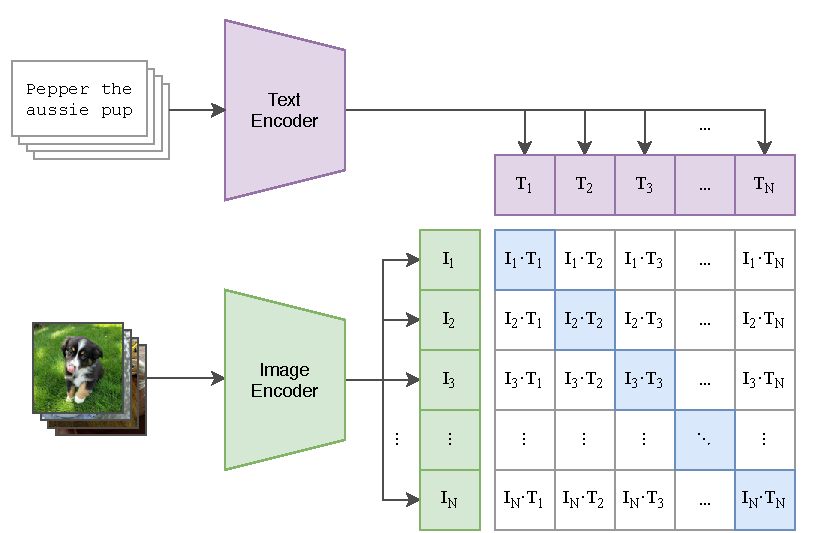
\includegraphics[width=0.45\linewidth]{figures/论文-图6-CLIP-方法.pdf}}
%   \subcaptionbox{CLIP可扩展性分析\label{fig:6-CLIP-Scaling}}
%     {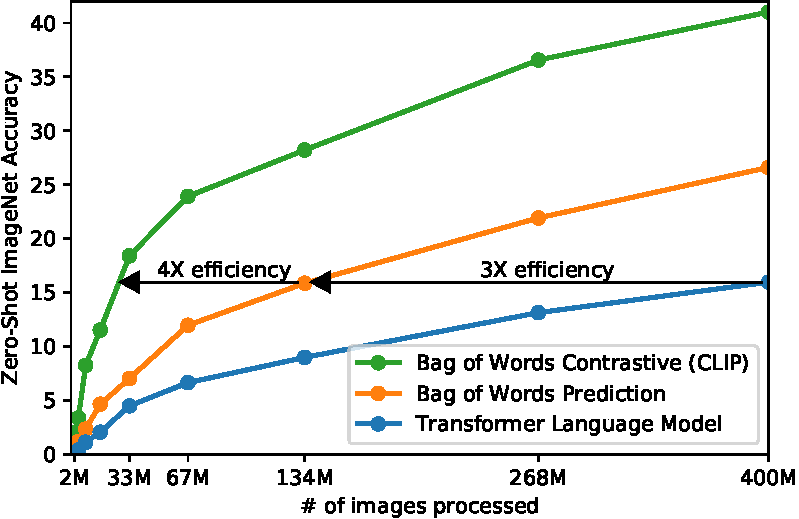
\includegraphics[width=0.45\linewidth]{figures/论文-图6-CLIP-效率.pdf}}
%   \caption{CLIP方法概览与可扩展性对比\cite{radford2021learning}}
%   \label{fig:6-CLIP-Method-Scaling}
% \end{figure}

% % 先不讨论LiT/SigLip/FLIP这些工作
% 在上述的局限性驱动下,以CLIP方法\cite{radford2021learning}为代表的视觉-语言多模态联合预训练方法逐渐被推广开来。如图\ref{fig:5-character-instance}(b)所示,这类方法\cite{radford2021learning,jia2021scaling,pham2023combined}可以看作是基于实例级对比学习的自监督预训练方法\cite{chen2020simple}的扩展。
% 在本文中,统一将这类利用互联网大规模图文配对数据进行实例级对比学习的方法统称为CLIP方法,而其中的代表工作即为OpenAI于2021年提出的CLIP模型\cite{radford2021learning}。
% 相比于字符级联合预训练方法,实例级方法不再要求模型在给定图像的情况下逐字符地预测文本信号,而是将配对的\{图像,文本\}信号视作对同一抽象对象的两种不同的描述方式。
% 实例级预训练方法的核心在于构建一个不同描述的共享表征空间,聚合属于同一对象不同描述的表征,分散属于不同对象不同描述的表征。因此,这种方法建模了图像与文本间的相对关系,不依赖图像与文本一一配对的强假设。
% 如图\ref{fig:6-CLIP-Method}所示,将一组$N$张图片记作$\mathcal{I}=\{I_1,\cdots,I_N\}$,将对应的一组$N$条替代文本记作$\mathcal{T}=\{T_1,\cdots,T_N\}$,记模型参数为$\theta$,实例级视觉-语言多模态联合预训练CLIP方法本质上在最大化如下概率估计:
% \begin{equation}
%     \max_{\theta}\left[\sum_{i=1}^{n}f(I_i,T_i)-\sum_{i\neq j;i,j\in[1,N]}f(I_i,T_j)\right]
%     \label{eq:instance-level}
% \end{equation}
% 其中$f$为某种距离度量方式,在CLIP方法中以视觉表征和语言表征的余弦相似度来表示。

% 从式\eqref{eq:instance-level}可以看出,实例级视觉-语言多模态联合预训练方法不再强调建模单个\{图像,文本\}对之间的对应关系,而是通过$N$个一组配对,对齐图像集合$\mathcal{I}$的表征空间和文本集合$\mathcal{T}$的表征空间。
% 尽管这类方法的监督信息量相比于字符级预训练方法较少,但它对数据质量的信噪比要求更低,更符合互联网大规模\{图像,替代文本\}对的实际特性,因此可以通过有效扩展训练样本数目来确保监督信息量充足。
% 如图\ref{fig:6-CLIP-Scaling}所示,CLIP模型证明这种方法相比于利用弱语义话题标签的弱监督方法有4倍的数据利用效率提升(绿色线与橙色线),而相比于字符级预训练方法则有12倍的数据利用效率提升(绿色线与蓝色线)。
% % 同时,实例级语言监督方法从字符序列长度不同的文本中得到的训练信号信息量一致,不存在某些图像学习不平衡导致的收敛不充分问题,也不存在序列长度不均衡带来的实现效率问题。
% 此外,实例级视觉-语言多模态联合预训练方法直接对齐了视觉表征与语言表征,因此为图文检索、物体识别、模态转换等下游任务提供了重要帮助。
% % 天然提供了一项额外好处:\todo{简单的大规模检索算法和零样本开放集合识别} % 开放集合识别貌似基于回归的办法也可以做。可以提检索简化了识别(把open end的映射问题转为排序问题),对物体检测、语义分割都有帮助
% 综上所述,实例级视觉-语言多模态联合预训练方法具备高效的数据利用效率和大规模扩展的潜力。同时CLIP方法作为一种基于语言监督的视觉模型预训练方法对视觉模型训练研究同样有深刻影响。
% !TeX root = ../main.tex
\chapter{基于高质量图像分类数据扩展的预训练方法}
\label{cha:iclip}
\label{sec:iclip-intro}
语言-图像对比学习方法通过对比学习框架在图文对数据中寻找正负样本对进行训练。其中图像及对应替代文本构成正样本对,该图像与其他替代文本构成负样本对。互联网数据中的替代文本来源多样,包含丰富的语义信息,使模型能够学习文本中的类别和属性与图像的关联关系,从而具备零样本开放集合图像识别能力。
然而,如图\ref{fig:iclip-overall}左侧所示,自动爬取的互联网图文对数据没有经过额外的人工标注或校对,往往包含图文无关的噪声(如相机参数、推广信息等),以及关联关系模糊、区分性不强的图文对数据。这些噪声数据会影响视觉表征对语义概念的建模效果,降低表征的判别能力。一般基于图像分辨率、文本长度过滤的启发式规则\cite{sharma-etal-2018-conceptual,changpinyo2021conceptual}比较简单,无法有效去除语义层面的噪声。因此,扩展高质量数据源并降低数据噪声的影响,是提升CLIP方法预训练效果的重要方向,也是本章的研究目标。

\begin{figure}
  \centering
  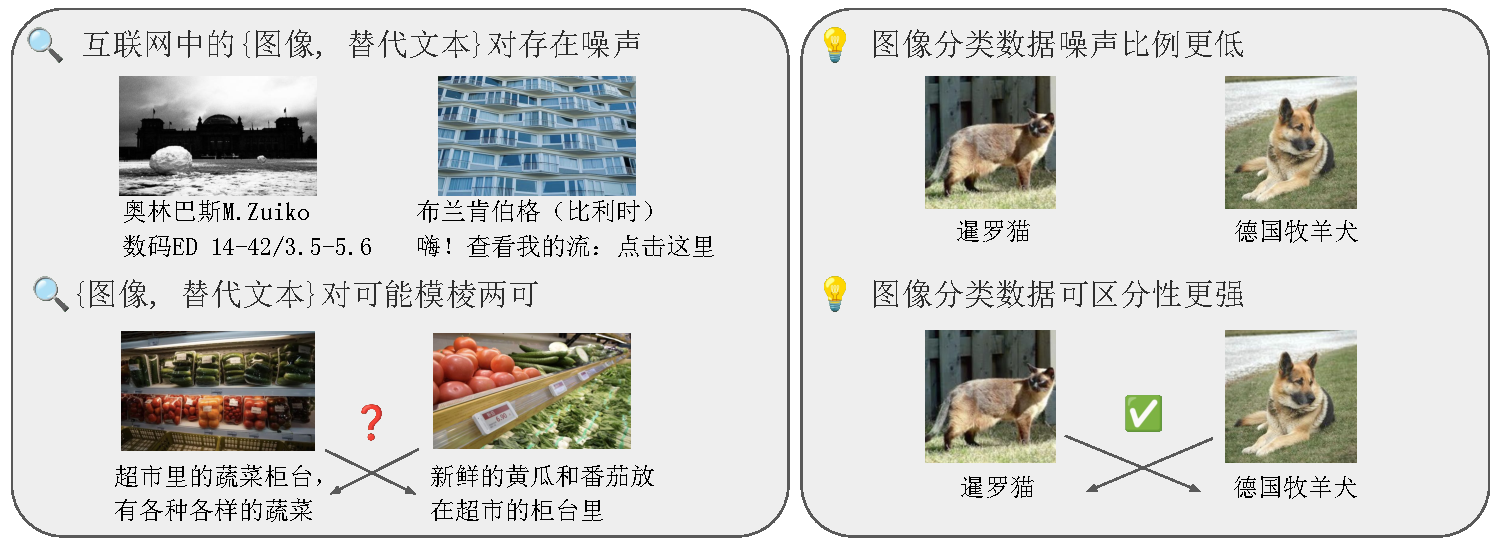
\includegraphics[width=1.0\linewidth]{figures/论文-iCLIP-概要.pdf}
  \caption{互联网图文对数据与图像分类数据的对比}
  \label{fig:iclip-overall}
\end{figure}

% 拜读了zl大哥DNL的部分,没想到引言部分是直接翻译过来的
\section{引言}
本章提出将对比学习思想扩展到其他图像及其标注信息配对数据中,从而合理利用已有的人工标注数据作为互联网图文对数据的补充,以实现不同标注形式的预训练数据的有效融合。
这种方式一方面为语言-图像对比学习方法提供额外的训练信号和图像样本,另一方面可以使用这些经过人工校对的精确标注信号作为视觉表征的准确锚定,增强其判别效果,使视觉表征与语言表征的联系更加紧密。
本章主要考虑有监督图像分类任务及其对应数据集作为语言-图像对比学习方法使用的图文对数据集的补充。
图像分类任务是一个典型的视觉预训练任务,其训练目标是在给定一组固定的预定义类别集合的情况下,将每一张输入图像划归到对应的类别。
作为有监督视觉预训练方法中最常使用的任务,研究界积累了相当多的公开图像数据。
如图\ref{fig:iclip-overall}右侧所示,广泛使用的ImageNet数据集\cite{deng2009imagenet}仔细标注了1400余万张图像,并将它们分为21841个不同的类别。其中每个类别都通过WordNet\cite{miller1995wordnet}语义网络提供了一个清晰的分类标准。因此图像分类任务的标注质量更高,同时具有明确的语义含义,更不容易出现不同的图像与标注之间混淆的情况,非常适合作为互联网图文对数据集的补充。
% 如果找到一种办法能有效利用这些现有的图像数据及其标注信息,并在实例级视觉-语言预训练方法中统一起来,将有效地提升整体数据的信噪比,并改善互联网图像文本对噪声导致的图文关联模糊问题。
% 同时,传统的图像分类任务往往仅限于一组预定义的固定类别集合,而CLIP方法天然具有开放类别的物体识别能力,这种表征融合的方法也很好地弥补了图像分类方法的不足。

% 本章将CLIP方法中的\{图像,文本\}实例级对比学习方法扩展到\{图像,文本,类别\}的三元组,在结合这两种视觉预训练方法的同时,充分利用对应的训练数据。
% 作为预实验,本章首先尝试了一个简单的多任务学习框架。该框架使用一个共享的视觉模型,并分别使用一个线性分类器进行图像分类任务训练和一个语言模型进行实例级多模态联合预训练。此时,\{图像,文本,类别\}的三元组关系通过分别建模\{图像,文本\}和\{图像,类别\}关系来实现。
% 虽然提升效果比较微弱,这种简单的多任务表征融合方法已经能够使两个单独的任务获益,但这一实验结果促进了本章沿着该方向的进一步探索。

因此本章探讨了如何有效地从语言-图像对比学习方法的角度重新理解传统的有监督图像分类方法。第一个尝试是将图像分类方法的损失函数和语言-图像对比学习方法的损失函数统一。
对比两者损失函数形式后可以发现,两种训练方法都可以被视作特殊的分类形式,其中前者是固定类别集合的分类,后者是正负样本对间的分类。
但两者仍然有几个主要区别:
1)损失函数形式不同。图像分类方法通常采用基于内积相似度的交叉熵损失函数,而语言-图像对比学习方法则使用基于余弦相似度的InfoNCE损失函数\cite{oord2018representation}。前者拟合能力更强,而后者对类别泛化更加友好。
% 1)损失函数形式不同。图像分类方法通常使用拟合能力较强的线性损失分类器。%由于线性损失的非归一化性质,该分类器驱动下的模型往往具有更好的拟合能力。
% 而语言-图像对比学习方法则采用对新类别泛化性更好的余弦损失分类器\cite{cao2020parametric,DengArcFace,wang2018cosface}。
2)分类器权重的参数化方法不同。图像分类方法采用直接类别参数化的分类器,而语言-图像对比学习方法则使用语言模型重参数化分类器。前者适合固定类别分类任务,后者适合多变类别分类任务。
% 图像分类方法只处理固定类别集合分类任务,可以直接优化各个类别的中心权重。而语言-图像对比学习方法则使用语言模型来建模不同文本中包含的语义信息,可以理解为通过语言模型重参数化了各个类别的中心权重。这种共享语义表征建模方式允许对不同文本语义之间的内部关系进行建模以增强对不同概念间关系的理解。同时这种方式可以处理预训练过程中未曾出现的概念信息,实现开放集合图像识别任务。
因此本章提出修改图像分类损失函数方法,从而与语言-图像对比学习方法统一。

除了统一损失函数形式之外,本章的第二个尝试是借助外部专家知识库增强数据,弥补图像分类数据和图文对数据在标注信息语义丰富度上的差异。
图像分类数据中提供语义信息的类别标签为求简洁明确,通常以一个或几个单词来表示。
但不同的类别标签之间可能有概念上的重叠,这使得它们在指代特定概念时存在有歧义情况。而图文对数据中提供语义信息的替代文本则通常是一个包含丰富语义的完整句子。这种语义信息密度的差异影响了语言模型的学习效果。
本方法利用了字典、百科等外部知识库来为图像分类数据中的类别标签提供更丰富的语义信息,包括类别定义、形象描述、与其他概念的关联和区别等等。这个过程就像人类通过真实示例和字典中的解释来学习新单词或概念,同时建模了这些新概念与其他概念间的关系。
% 为这些类别名称提供了为模型训练提供了更多监督信号。
得益于在图像分类方法中引入语言模型重参数化分类器的设计,这种包含了复杂语义信息的外部知识可以通过语言模型来直接建模,从而更好地从语言-图像对比学习方法的角度重新理解图像分类方法。

% 图像分类任务中类别名称为力求简洁明确,通常以一个或几个单词来表示。但不同的类别名称之间可能有概念上的重叠,这使得类别名称在指代特定语义时存在有歧义或多义的情况。
% 例如,ImageNet数据集中有一类别为``夜晚的鸟''(``night bird''),这一类别名称就与数据集中出现的其他类别有概念上的重叠,包括数据集中出现的``猫头鹰''(``owl'')、``夜莺''(``nightingale'')等类别。此外,``nightingale''还与知名历史人物弗洛伦丝·南丁格尔(``Florence Nightingale'')有词汇上的重合。% https://storage.googleapis.com/bit_models/imagenet21k_wordnet_lemmas.txt
% 与此同时,CLIP联合预训练方法使用图文对数据训练,其中的替代文本往往是包含丰富语义的完整句子。
% 为了进一步弥合图像分类任务和实例级视觉-语言多模态联合预训练任务之间的差距,
整合这些技术后,本章提出了一个新的预训练方法,称为iCLIP。iCLIP方法从损失函数和标注信息语义丰富度两个角度出发,以语言-图像对比学习方法重新理解传统的有监督图像分类方法,从而在基于互联网图文对数据的语言-图像对比学习预训练中得以有效融合高质量的图像分类数据,降低了数据噪声影响的同时增加了预训练可利用数据来源。

实验结果首先表明,尽管线性损失分类器和分类器权重直接参数化方法是图像分类方法的默认形式,但是将语言-图像对比学习方法的余弦损失分类器和语言模型重参数化分类器引入图像分类方法不会影响图像分类任务本身的学习效果。这一结果支持iCLIP方法用语言-图像对比学习思想有效融合两种方法的数据源进行预训练。
此外,iCLIP方法提出的外部专家知识库增强方法有效缩小了图像分类数据和图文对数据在标注信息的语义丰富度上的差距。实验表明将外部知识作为文本前缀或后缀与类别标签组合,即可显著提高模型的零样本开放集合图像识别任务效果,并改进了模型在零样本图文跨模态检索任务上的表现。
相比于简单的多任务预训练方法,这种从损失函数和标注信息语义丰富度角度重新理解图像分类方法,有效融合两种预训练方式的iCLIP方法显著提升了视觉表征与语言表征的对齐效果,并增强了视觉表征的语义判别能力。
与此同时,在迁移到下游视觉任务中时,iCLIP方法表现也更佳。相比于单一图像分类方法或单一语言-图像对比学习方法,iCLIP方法在少样本图像识别\cite{imagnettransfer}、ADE20K数据集\cite{zhou2019ade}语义分割、LVIS数据集\cite{gupta2019lvis}长尾类别物体检测和Kinetics-400数据集\cite{kay2017kinetics}视频动作识别等任务上均展现出优势。
% 这表明以实例级视觉-语言多模态联合预训练CLIP方法的形式重新理解和建模图像分类任务没有额外损失,因此可以

% 本章在不同规模的数据集组合实验中对该方法进行了验证。结果表明更高精度的图像分类数据明显增强了CLIP预训练对效果,使其在零样本物体识别和图文跨模态检索任务中的表现明显优于单独使用其中一种预训练方法或简单的多任务学习方法。

综上所述,本章的主要内容安排如下:
\begin{itemize}
    \item 第\ref{sec:iclip-intro}节讨论了互联网图文对数据中的标注噪声问题和引入高质量有标注数据,比如图像分类数据的潜在好处并介绍了从损失函数形式和标注信息语义丰富度两个角度,重新以语言-图像对比学习思想理解图像分类任务的方法。
    \item 第\ref{sec:iclip-method}节介绍了本章的研究方法,包括从对比学习角度理解图像分类任务的具体设计以及引入外部专家知识库对类别语义进行增强的具体方法等,并提出统一预训练方法iCLIP的具体实现。
    \item 第\ref{sec:iclip-result}节介绍了本章的实验设置、评测指标和实验结果,以及针对各模块的消融实验结果。
    \item 第\ref{sec:iclip-summary}节对本章内容进行了总结。
\end{itemize}

\section{研究方法}
在第\ref{sec:iclip-compare}节中首先对比了图像分类方法和语言-图像对比学习方法的损失函数。之后,在第\ref{sec:iclip-adapt-classification}节中提出从对比学习角度理解图像分类方法的具体设计,并在第\ref{sec:iclip-adapt-external}节中讨论了引入外部专家知识库对图像类别语义进行增强的做法。最后在第\ref{sec:iclip-unify}节中介绍了有效融合的统一预训练方法iCLIP的具体形式。

\label{sec:iclip-method}
\begin{figure}
  \centering
  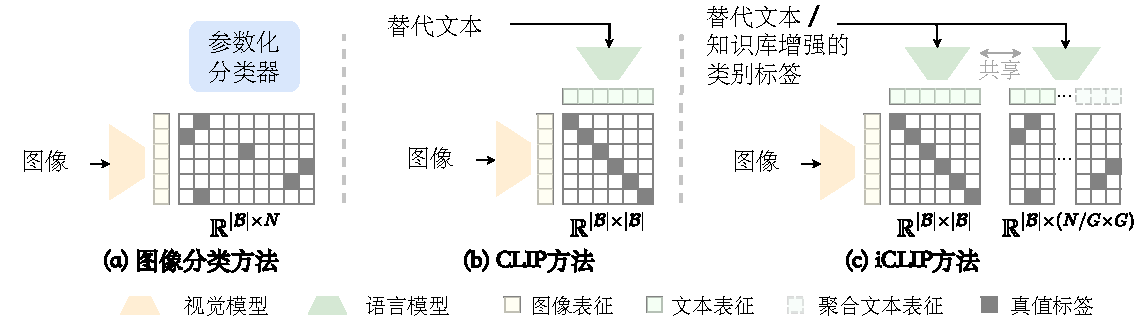
\includegraphics[width=1.0\linewidth]{figures/iclip-compare.pdf}
  \caption{图像分类方法、CLIP方法和融合后的iCLIP方法示意图}
  \label{fig:iclip-compare}
\end{figure}
\subsection{图像分类方法和语言-图像对比学习方法对比}
\label{sec:iclip-compare}
\paragraph{图像分类方法的损失函数} 图像分类方法的训练数据$D^{c}$是一组\{图像,类别序号\}对,记为$D^{c}={(I_{i}, C_{i})}_{i=1}^{|D^{c}|}$,其中$I_{i}$和$C_{i}$分别表示第$i$个图像和对应的类别序号标注。图像分类方法的训练目标是使用视觉模型$\theta_{I}$和直接参数化的类别分类器$h_{c}$预测给定图像的类别序号。分类器$h_{c}$是一个$N×H$大小的线性层,其中$N$是分类数据中的总类别数,$H$是视觉模型$\theta_{I}$输出的图像表征维度。分类器的参数记为$W$。图\ref{fig:iclip-compare}(a)展示了批大小为$\mathcal{B}$时的情况。
视觉模型$\theta_{I}$将每个图像$I_{i}$转换为图像表征:$v_{i}=\theta_{I}(I_{i})$,而分类器$h_{c}$则通过计算$W$和$v_{i}$之间的内积来预测该图像在所有类别上的概率分布$P_{i}$,且$P_{i}\in R^{N}$。最后,图像分类方法在$P_{i}$和$C_{i}$之间应用交叉熵函数来计算训练损失,公式化为:
\begin{equation}
 \mathcal{L}=-\frac{1}{\left|\mathcal{D}^{c}\right|} \sum_{\left(I_{i}, C_{i}\right) \in \mathcal{D}^{c}} \log \frac{\exp \left(W_{C_{i}} \cdot v_{i}\right)}{\sum_{j=1}^{N} \exp \left(W_{j} \cdot v_{i}\right)},
 \label{eq:iclip-classification}
\end{equation}
其中$W_{j}$是分类器参数中第$j$个类别对应的中心权重。

\paragraph{语言-图像对比学习方法的损失函数} 语言-图像对比学习方法的训练数据$D^{a}$是一组\{图像,替代文本\}对,记为$D^{a}={(I_{i}, T_{i}^{a})}_{i=1}^{|D^{a}|}$,其中$I_{i}$和$T^{a}_{i}$分别表示第$i$个图像和对应的文本标注。
语言-图像对比学习方法的训练思想是通过视觉模型$\theta_{I}$和语言模型$\theta_{T}$缩小配对的图像表征和文本表征之间的距离,同时扩大未配对的图像表征和文本表征之间的距离。
图\ref{fig:iclip-compare}(b)展示了批大小为$\mathcal{B}$时的情况。
语言-图像对比学习方法首先将图像$I_{i}$和替代文本$T_{i}^{a}$通过视觉模型$\theta_{I}$和语言模型$\theta_{T}$转换为对应表征$v_{i}$和$s_{i}$,也即$v_{i}=\theta_{I}(I_{i})$且$s_{i}=\theta_{T}(T_{i}^{a})$。接着,语言-图像对比学习方法应用InfoNCE对比损失函数来计算训练损失。以当前图像$I_{i}$为中心的损失函数公式化为:
\begin{equation}
 % \mathcal{L}=-\frac{1}{\left|\mathcal{D}^{a}\right|} \sum_{\substack{\left(I_{i}, T_{i}^{a}\right) \\ \in \mathcal{D}^{a}}} log \frac{exp \left(cos \left(\theta_{T}\left(T_{i}^{a}\right), v_{i}\right) / \tau\right)}{\sum_{T_{j}^{a} \in \mathcal{T}^{a}} exp \left(cos \left(\theta_{T}\left(T_{j}^{a}\right), v_{i}\right) / \tau\right)}
 \mathcal{L}=-\frac{1}{\left|\mathcal{D}^{a}\right|} \sum_{\left(I_{i}, T_{i}^{a}\right) \in \mathcal{D}^{a}} \log \frac{\exp \left(\cos \left(s_{i}, v_{i}\right) / \tau\right)}{\sum_{T_{j}^{a} \in \mathcal{T}^{a}} \exp \left(\cos \left(s_{j}, v_{i}\right) / \tau\right)},
 \label{eq:iclip-clip}
\end{equation}
其中$\cos(\cdot, \cdot)$表示两个表征之间的余弦相似度,$\mathcal{T}^{a}$是当前批数据中的所有文本标注作为对比对象,包括一个和当前图像$I_{i}$配对的正样本和$\mathcal{B}-1$个不配对的负样本,而$\tau$是一个缩放相似程度的超参数。由于语言-图像对比学习方法对图像信息和文本信息的建模对称性,在训练过程中还有一个以当前替代文本$T_{i}^{a}$为中心的损失函数,并取两者平均。该损失函数和公式\eqref{eq:iclip-clip}形式相似,只是将对比对象从当前批数据中的所有文本标注替换为所有图像。
 
\paragraph{损失函数对比} 比较图像分类任务和语言-图像对比学习方法的损失函数,可以看出两种训练方法都可以被视作分类方法的一种,前者在固定大小的图像类别中进行分类,后者则在给定批数据中的所有文本标注中进行分类。但是它们之间仍有三个主要区别:
\begin{itemize}
    \item 两种方法在损失函数形式上有区别。图像分类方法使用基于内积相似度的线性损失函数。由于内积相似度是一种非归一化的相似度,可以通过表征和参数的模长提供更多信息,该损失函数下的分类器往往具有更好的拟合能力。而语言-图像对比学习方法则采用基于余弦相似度的损失分类器。这种损失函数下的分类器更关注方向信息,对新类别泛化性更好\cite{cao2020parametric,DengArcFace,wang2018cosface}。
    % 1)损失函数形式的区别。图像分类任务通常采用基于内积相似度的交叉熵损失,而语言-图像对比学习方法则使用基于余弦相似度的InfoNCE损失函数\cite{oord2018representation}。
    \item 两种方法在分类器权重的参数化方法上有区别。图像分类方法采用直接参数化的类别分类器,这种分类器可以直接优化各个类别的中心权重,但只处理固定类别集合的分类任务。而语言-图像对比学习方法则使用一个语言模型来建模不同文本标注中包含的语义信息,可以理解为通过语言模型重参数化分类器权重。这种类别间共享参数的方式允许分类器构建不同类别间的复杂关系,增强对不同语义概念的理解。同时这种方式借助语言模型的灵活性,可以建模训练过程中未曾出现过的概念信息,从而实现开放集合图像识别的目标。
    % 图像分类方法采用直接参数化的类别分类器,而语言-图像对比学习方法则使用语言模型重参数化分类器。
    \item 两种方法在标注信息的语义丰富度上有区别。图像分类方法使用的类别序号仅仅区分了不同类别,并不包含任何语义信息,而语言-图像对比学习方法使用的文本标注是包含丰富语义的完整语句,提供了关于图像内容的详细描述。
\end{itemize}


\subsection{从对比学习角度重新理解图像分类方法}
\label{sec:iclip-adapt-classification}
为了有效融合图像分类任务和语言-图像对比学习方法,从而运用高质量图像分类数据进行增强,本节讨论了从对比学习角度重新理解图像分类方法的两个调整措施:对齐损失函数形式和统一分类器参数化方法。整体流程如图\ref{fig:iclip-adapt}所示。
% todo: 现在的写法里,a.2 & a.3要画成对齐损失函数和分类器参数化方法。

\begin{figure}
  \centering
  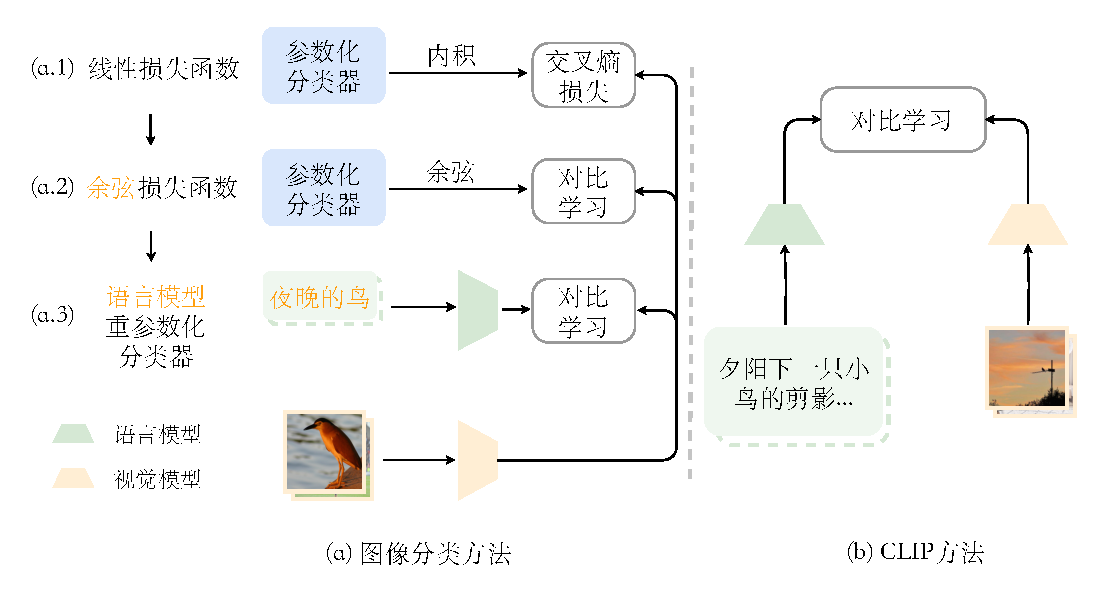
\includegraphics[width=1.0\linewidth]{figures/iclip-adapt-v2.pdf}
  \caption{从对比学习角度重新理解图像分类方法的调整措施}
  \label{fig:iclip-adapt}
\end{figure}

\paragraph{基于余弦相似度的图像分类损失函数} 如公式\eqref{eq:iclip-classification}所示,图像分类方法首先得到视觉表征$v_{i}$与直接参数化的类别分类器$h_{c}$之间的内积相似度,并归一化为概率分布$P_i$之后,与独热化类别序号之间应用交叉熵损失函数。这个损失函数与语言-图像对比学习方法中使用的InfoNCE对比损失函数相似但不一致,使得两个方法无法有效融合。
为了解决这个差异,本节提出在图像分类方法中引入余弦相似度,并同样添加一个控制概率分布的温度系数$\tau$,其损失函数形式就与InfoNCE对比损失函数形式一致,只是采样的负样本变成了其他类别。基于余弦相似度的图像分类损失函数公式化为:
\begin{equation}
    \mathcal{L}=-\frac{1}{\left|\mathcal{D}^{c}\right|} \sum_{\left(I_{i}, C_{i}\right) \in \mathcal{D}^{c}} \log \frac{\exp \left(\cos \left(W_{C_{i}}, v_{i}\right) / \tau\right)}{\sum_{j=1}^{N} \exp \left(\cos \left(W_{j}, v_{i}\right) / \tau\right)}.
    \label{eq:iclip-cosine}
\end{equation}

余弦相似度是度量学习\cite{nguyen2010cosine}中的一种常见做法。通过在图像分类方法中引入余弦相似度,图像分类方法与语言-图像对比学习方法在损失函数形式方面保持一致。后续实验表明,这种基于余弦相似度的图像分类方法可以取得与传统基于线性相似度的图像分类方法相当的分类表现。

\paragraph{在图像分类方法中引入语言模型重参数化分类器权重} 虽然公式\eqref{eq:iclip-cosine}对齐了两种方法的损失函数形式,但是两种方法使用的图像标注信息,也即图像分类数据中的类别序号和图文对数据中的文本内容,仍分别由直接参数化的类别分类器$h_{c}$和语言模型$\theta_{T}$进行建模。
在这种方式下,视觉模型接收到的训练信号由两个分类器单独给出,而且不同的语义概念信息无法在两个分类器间共享,无法充分利用文本语义概念丰富性和类别信息准确性的结合优势。
% 语言模型的学习信号并没有获得引入图像分类数据后的收益。
后续实验也表明,这种简单融合的分类器分离方案没有充分利用图像分类数据和图文对数据的优势,影响了预训练模型视觉表征与语言表征的对齐效果。

为了解决这个问题,本节重新引入图像类别中蕴含的语义信息,并提出用语言模型重参数化分类器建模图像分类任务。
如前文所述,图像分类数据集ImageNet中的每一个类别序号都对应了语义网络WordNet中的一个同义词集合,因此图像分类任务中的类别序号都有其对应的标签文本。因此,本节提出用共享的语言模型$\theta_{T}$重参数化图像分类方法的分类器权重。
具体而言,先通过语义网络WordNet将类别序号$C_{i}$替换为其对应的标签文本$M_{i}$,并通过语言模型$\theta_{T}$提取$N$个不同类别对应的文本表征,从而动态生成分类器权重$W$。在图像分类方法中引入语言模型重参数化分类器权重后的公式为:
\begin{equation}
    \mathcal{L}=-\frac{1}{\left|\mathcal{D}^{c}\right|} \sum_{\left(I_{i}, M_{i}\right) \in \mathcal{D}^{c}} \log \frac{\exp \left(\cos \left(\theta_{T}\left(M_{i}\right), v_{i}\right) / \tau\right)}{\sum_{j=1}^{N} \exp \left(\cos \left(\theta_{T}\left(M_{j}\right), v_{i}\right) / \tau\right)}.
    \label{eq:iclip-wo-dictionary}
\end{equation}

此时,语言模型$\theta_{T}$不仅有效捕获高区分度的标签文本语义特征,还能整合丰富的文本语义信息。
这一改进使得语言-图像对比学习方法可以更好地利用图像分类数据进行增强。

\subsection{外部专家知识库增强图像类别语义方法} 
\label{sec:iclip-adapt-external}
\begin{figure}
  \centering
  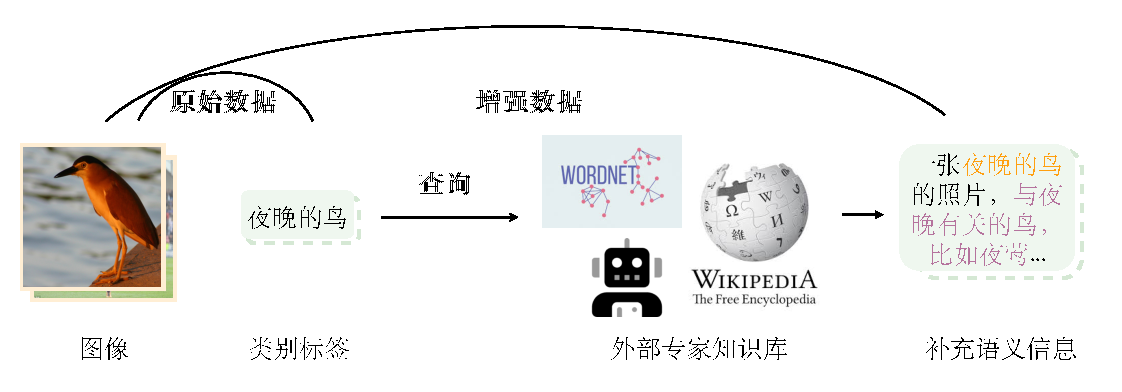
\includegraphics[width=1.0\linewidth]{figures/iclip-knowledge.pdf}
  \caption{外部专家知识库对类别标签的增强方法}
  \label{fig:iclip-knowledge}
\end{figure}
第\ref{sec:iclip-adapt-classification}节中通过引入基于余弦相似度的图像分类损失函数和语言模型重参数化分类器权重的方式,实现了从对比学习角度重新理解图像分类方法,并在很大程度上统一了两个不同的方法。
但是两种方法使用的数据在标注信息的语义丰富度上仍有较大区别。图像分类方法中类别对应的标签文本$M_i$来自于语义网络中的同义词集合。为保持简洁明确,通常每个类别均以一个或几个单词来表示。与此同时,语言-图像对比学习方法使用的图文对数据中,每个图像对应的文本标注包含了丰富的语义信息,其通常以完整语句的形式描述了图像中存在的物体对象、物体属性、对象间关系、上下文背景信息等等。
因此,需要进一步在标注信息的语义丰富度上进行对齐,减少两种方法之间的差异,增强预训练模型的学习效果。

为了增强图像分类数据中的标注信息的语义丰富度,本节提出引入外部专家知识库进行增强的方法。流程如图\ref{fig:iclip-knowledge}所示。具体而言,对于分类数据中的每一个类别,该方法都从外部专家知识库中检索并构造相关的知识信息作为标签文本的补充。这个知识库可以是字典、百科、知识图谱或者大语言模型。
在实际实现中,本节利用了语义网络WordNet作为外部专家知识库。如前文所述,每个分类类别在语义网络中都对应了一个同义词集合,而语义网络类似字典,为每个同义词集合编写了一条详细描述,用以明确定义该同义词集合所表达的语义概念,并可能提供一些相关知识以及与其他同义词之间的关联关系作为补充,非常适合作为外部知识引入。
得到每个类别对应的详细描述之后,该方法将其与类别标签文本组合并添加一些语法模板,使得新句子更加流畅易读,即可构成语义丰富度增强后的类别标注。这种增强后的标注称为图像类别描述,记作$\mathcal{T}^{c}$。
以“银行”类别为例,语义扩充后的类别标注为:“这是一张银行的图片,关于银行的定义是接受存款并将资金用于贷款活动的金融机构”。
% https://web.stanford.edu/~jurafsky/slp3/G.pdf

% 此外,在增强后的句子中。知识库增强后的类别标签形式为:
% \begin{equation}
%     \mathcal{T}^{c}=\{\text{TEMPLATE}\}_{C_i},\{\text{NAME}\}_{C_{i}},\{\text{DESCRIPTION} \}_{C_{i}}
%     \label{eq:iclip-format-label}
% \end{equation}

 这种外部专家知识库增强后的类别描述具有与图文对数据的文本信息相似的语义丰富度,从而进一步对齐了图像分类方法与语言-图像对比学习方法,以充分利用两种数据源。
 此外,这些外部专家知识库为每个图像类别引入了更多细节信息,能够减少因为原始的类别标签文本之间概念重叠造成的混淆现象。由于图像类别的标签文本本身长度较短,在类别数目较多的情况下容易存在指代特定语义时出现歧义的现象。
 例如,图像分类数据集ImageNet中有一类别为“夜晚的鸟”(“night bird”),这一类别名称就与数据集中出现的其他类别有概念上的重叠,包括“猫头鹰”(“owl”)和“夜莺”(“nightingale”)等类别。此外,“夜莺”的英文名称还与知名历史人物弗洛伦斯·南丁格尔护士(“Florence Nightingale”)有词汇上的相似。
 因此,仅仅依靠图像类别的标签文本难以区分不同类别间的细微差别,会影响模型在预训练过程中学习到更精确的概念表示。
 但是语义网络中将“夜晚的鸟”详细描述为“任何与夜相关的鸟类:猫头鹰、夜莺、夜鹰......”,提供了关于该类别更明确的语义信息。因此引入外部专家知识库的方法不仅在标注信息语义丰富度上与图文对数据对齐,还有助于模型区分不同概念并建立相关关系,进一步增强视觉表征的判别能力。

% 图像分类任务中类别名称为力求简洁明确,通常以一个或几个单词来表示。但不同的类别名称之间可能有概念上的重叠,这使得类别名称在指代特定语义时存在有歧义或多义的情况。
% 例如,ImageNet数据集中有一类别为``夜晚的鸟''(``night bird''),这一类别名称就与数据集中出现的其他类别有概念上的重叠,包括数据集中出现的``猫头鹰''(``owl'')、``夜莺''(``nightingale'')等类别。此外,``nightingale''还与知名历史人物弗洛伦丝·南丁格尔(``Florence Nightingale'')有词汇上的重合。% https://storage.googleapis.com/bit_models/imagenet21k_wordnet_lemmas.txt
% 与此同时,CLIP联合预训练方法使用图文对数据训练,其中的替代文本往往是包含丰富语义的完整句子。
% 为了进一步弥合图像分类任务和实例级视觉-语言多模态联合预训练任务之间的差距,

\subsection{有效融合的统一预训练方法iCLIP}
\label{sec:iclip-unify}
通过从对比学习角度重新理解图像分类方法并引入外部专家知识库增强图像类别语义,图像分类任务在损失函数形式、分类器权重参数化方法和标注信息语义丰富度三个方面,与语言-图像对比学习方法对齐。因此,本节提出了一个有效融合的统一预训练方法iCLIP,达到增强视觉表征的语义丰富度的效果。
如图\ref{fig:iclip-compare}(c)所示,iCLIP方法将高质量图像分类数据引入语言-图像对比学习预训练中,并用对比学习方法统一建模,其形式为:
\begin{equation}
   \mathcal{L}=-\frac{1}{|\mathcal{D}|} \sum_{\left(I_{i}, T_{i}\right) \in \mathcal{D}} \log \frac{\exp \left(\cos \left(\theta_{T}\left(T_{i}\right), v_{i}\right) / \tau\right)}{\sum_{T_{j} \in \mathcal{T}} \exp \left(\cos \left(\theta_{T}\left(T_{j}\right), v_{i}\right) / \tau\right)},
   \label{eq:iclip-unified}
\end{equation}
其中$D$是由图像分类数据集$D^{c}$和图文对数据集$D^{a}$组成的集合。而对比样本集合$\mathcal{T}$表示所有类别经过外部知识库增强后的标签文本集合$\mathcal{T}^{c}$或者当前批数据中的替代文本集合$\mathcal{T}^{a}$。因此,其中的文本信息$T_{j}$可以是从$\mathcal{T}^{c}$中采样的图像类别描述,或者从$\mathcal{T}^{a}$中采样的替代文本。
值得注意的是,在这个融合后的预训练方法中,视觉模型$\theta_{I}$和语言模型$\theta_{T}$在图像分类数据集和图文对数据集之间共享。这种融合方式使得模型能够借助图像分类数据集学习判别性更强的视觉表征,同时从图文对数据集中对齐更丰富的语义概念,增强了预训练效果。

\paragraph{通过分布式计算进行实现上的优化} 在iCLIP方法中,每个图像类别描述对应的语言表征由同一个语言模型动态生成,以替代直接优化分类器权重$W$的传统做法。当图像分类数据集中的类别数量$N$较小时,计算开销较小。
但是,对于图像类别数量$N$较大的数据集,例如包含2万多个类别的ImageNet数据集全集,在单次随机梯度下降过程中语言模型需要提取$N$个图像类别描述对应的语言表征,对训练速度产生了较大影响。
为了使iCLIP方法适用于尽可能多的图像类别,本节参考数据并行方法,实现了分布式训练策略\cite{chen2020simple}来降低由于图像类别增多造成的计算开销。
具体来说,iCLIP方法将$N$个引入外部专家知识库增强后的图像类别描述均匀地分布在$G$个数据并行的模型实例上,使得每个模型实例只需要提取$N/G$个图像类别描述对应的语言表征。在计算公式\eqref{eq:iclip-unified}的损失函数时,每个模型实例会从其他模型实例中的输出中收集对应类别的语言表征以构建完整集合,再与分配给当前模型实例的图像进行对比学习。
这种分布式计算方法显著降低了语言模型提取表征的计算成本,并节约了$(G-1)/G$的显存开销,使得iCLIP方法能够处理图像类别数量较大的分类数据集。

\section{实验结果}
\label{sec:iclip-result}
本节将有效融合的统一预训练方法iCLIP,与单方法预训练基线和简单融合预训练基线进行比较。实验验证了引入高质量图像分类数据后对语言-图像对比学习方法的增强效果。
本节分别在百万、千万和亿级别数据规模上对iCLIP方法进行了验证,验证所提方法在不同的数据规模下均能表现出更优性能,并在小规模数据集上进行详细的消融实验。
为比较增强前后语言-图像对比学习方法预训练效果,本节采用零样本开放集合图像识别任务和零样本图文跨模态检索任务对各个方法进行比较,反映了不同方法的视觉表征与语言表征对齐水平和视觉表征对语义概念的覆盖程度。与此同时,本节还在各类视觉下游任务上验证不同预训练方法的微调效果,包括图像语义分割任务、长尾类别物体检测任务和视频动作识别任务。

\subsection{实验设置}
\label{sec:iclip-exp-setting}
本节首先详细说明预训练过程中使用的数据集和实验设置,以及评测方法。

\paragraph{预训练实验数据和设置} 本节使用百万、千万和亿级别三种不同规模的数据集组合进行预训练实验,以充分比较不同方法在不同规模下的表现。
\begin{itemize}
    \item 在百万级图像规模的实验设置中,本节选用常用的ImageNet 1K子集(简称为IN-1K)和Conceptual Caption 3M数据集\cite{sharma-etal-2018-conceptual}(简称为CC-3M)作为预训练数据。作为图像分类数据,IN-1K数据集大约有128万张图片,并包含1000种不同的图像类别,而CC-3M数据集则是图文对数据集,大约有300万张图片,每张图片有一个配对的替代文本。
    在模型结构方面,视觉模型采用Swin-Tiny\cite{Swin}结构,约有2800万个参数,并使用224x224像素的图片作为输入,而语言模型则采用BERT-Base\cite{BERT}结构,约有1亿2500万个参数,并最多使用77个词元的文本作为输入。视觉模型和语言模型分别通过视觉自监督方法MoBY\cite{MoBY}和语言自监督方法RoBERTa\cite{liu2019roberta}进行初始化,从而加速实验收敛速度,节约预训练的计算开销。
    在每一个批大小为$\mathcal{B}$的训练批次中,iCLIP方法分别从两个数据集采样一半的图像,因此两个数据源的总训练样本数相同。所有实验中的单模型实例的批大小为128张图像,并使用分布式数据并行方法在8个模型实例上并行训练了100轮。默认的学习率调度为余弦调度方法,其中前5轮会进行学习率预热至2e-4的最高学习率。在正则化方面,实验的权重衰减系数为0.01,并使用随机增强\cite{cubuk2020randaugment}的图像数据增强方法和比例为0.1的随机深度\cite{huang2016deep}方法,以增强模型的泛化性。
    \item 在千万级图像规模的实验设置中,本节选用ImageNet全集(简称为IN-22K)和YFCC 14M子集\cite{YFCC100M}(简称为YFCC-14M)作为预训练数据。作为图像分类数据,IN-22K数据集大约有1400万张图片,并包含2万多种不同的图像类别,而YFCC-14M数据集是YFCC图文对数据集\cite{YFCC100M}的常用子集,同样包含大约1400万张图片。相比于前一组预训练数据设置,该组实验数据规模扩大了一个数量级,以进一步验证iCLIP方法的在更大规模数据上是否仍然有效。
    在模型结构方面,视觉模型同样使用Swin-Tiny结构,而语言模型则和原始CLIP语言模型\cite{radford2021learning}结构相同,使用一个隐藏宽度为512,深度为12层的Transformer\cite{Transformer}结构,约有6300万个参数。本组实验中的视觉和语言模型均从随机初始化开始训练,以便与一些相关工作进行公平的比较。
    在该组实验中采用的单模型实例批大小为512张图像,并在16个模型实例上并行训练了32轮。由于该组实验预训练长度增加,需要更强的正则化方法以防止过拟合,因此将权重衰减增大为0.05,而其他正则化设置和实验设置与之前相同。% 最大学习率设为2e-4或8e-4。
    此外,为与单方法预训练基线进行公平比较,本组实验设置了两个数据规模相当的变体:1)从IN-22K数据集中去除属于IN-1K数据集类别的所有数据,构造新的图像分类数据集IN-21K,用于评估IN-1K数据集上零样本图像识别效果;2)从IN-21K数据集和YFCC-14M数据集中各采样一半数据进行组合,确保数据规模和训练开销与基线方法相同。
    \item 在亿级别图像规模的实验设置中,本节选用ImageNet全集和Laion-400M数据集\cite{schuhmann2021laion400m}作为预训练数据。Laion-400M数据集是一个从Common Crawl开源项目中收集的超大规模图文对数据集,包含大约4亿张来源各异、内容丰富的图像,可以充分验证iCLIP方法在超大规模数据组合下是否仍然有效。
    在该组实验设置中,视觉模型采用Swin-Base\cite{Swin}结构,约有8900万参数,而语言模型仍使用BERT-Base结构,并采用自监督方法对模型进行初始化。
    整个实验共训练10万个批次,其中单模型实例的批大小为192张图像,并采用64个数据并行的模型实例同时预训练。和前述实验设置略有不同,本组实验在每个批大小为192的训练批次中,分别从IN-22K数据集和Laion-400M数据集中采样64张和128张图像。因此,本组实验在图像分类数据集上完成约30轮训练,在图文对数据集上完成约2轮训练。
    在实验设置方面,本组实验同样使用余弦学习率调度方法,并使用前16700个训练批次进行学习率预热至到1e-3的最高学习率。在正则化设置方面,模型的权重衰减系数设置为0.05,随机深度比例设置为0.2,其他设置不变。
\end{itemize}

\paragraph{评测数据集和微调设置} 本节通过两种评测方法比较不同预训练方式的视觉表征训练效果,并在几种不同的微调任务中对不同预训练方法进一步对比。
\begin{itemize}
    \item 零样本开放集合图像识别任务是语言-图像对比学习方法的重要评测方式之一。本节在三个评测集上对比了不同预训练方法视觉表征的语义丰富度和泛化能力:1)IN-1K评测集及其变体IN-S评测集\cite{wang2019learningSketch}上的Top-1准确率,衡量了通用图像识别能力和视觉表征的健壮性;2)广泛使用的Kornblith-12评测集\cite{imagnettransfer}上的平均Top-1准确率,涵盖了12个不同领域的开放集合细粒度图像识别任务;3)UniCL\cite{unicl}方法中使用的14个细粒度图像识别任务的平均Top-1准确率,简称为UniCL-14泛化评测集。
    \item 领域内的图像识别任务是一种特殊的图像识别任务评测。一些预训练设置中包含了IN-1K训练数据集,因此在这些情况下在IN-1K和IN-S评测集上测试反映了不同方法在领域内的图像识别能力,不涉及开放集合识别能力。
    \item 零样本图文跨模态检索任务评测衡量了语言-图像对比学习方法的视觉表征与语言表征对齐效果。本节使用包含1000张图片的Flickr30K\cite{young2014flickr}(简称Flickr)评测集和包含5000张图片的MSCOCO\cite{chen2015microsoft}(简称COCO)评测集上对不同预训练方式进行比较,并展示不同方法在这两个评测集上的图像检索(简称为IR)和文本检索(简称为TR)的Top-1召回率。
    \item 在下游视觉任务上的微调表现反映了不同预训练方法视觉模型的泛化能力。本节首先评价了不同方法在少样本图像识别任务上的微调表现。该任务使用Kornblith-12数据集上的训练集对模型进行微调,并根据每个图像类别的训练样本数目不同构造了不同的评测方式。这项微调任务设置遵循了OpenAI CLIP\cite{radford2021learning}工作的原本设置:在微调过程中固定视觉模型不变,只微调额外的类别分类器,并报告平均Top-1准确率。
    其次,本节还在图像语义分割、长尾类别物体检测和视频动作识别视觉任务上对不同预训练方法进行了微调,并分别比较了不同方法在这些任务上的mIoU得分、检测框mAP得分和Top-1准确率。具体的微调设置如下。针对图像语义分割任务,本节使用MaskFormer~\cite{maskformer}方法作为微调框架在ADE20K\cite{zhou2019ade}数据集进行实验,将其视觉模型的窗口大小设为7,其他设置与其默认训练超参数配置一致,并展示了单尺度测试结果。对于长尾类别物体检测任务,本节使用了包含1203个不均匀分布物体类别的LVIS数据集\cite{gupta2019lvis},并采用广泛使用的Faster R-CNN\cite{ren2016faster}方法作为微调框架。其他微调设置与主流方法\cite{Swin}一致,包括24轮的训练时长、图像短边长度在480-800像素之间的多尺度训练,并报告单尺度检测框的测试结果。对于视频动作识别任务,本节采用Swin视觉模型的微调框架和设置,在Kinetics-400\cite{kay2017kinetics}数据集上微调30轮,并报告Top-1准确率。
\end{itemize}

\subsection{百万级图像规模的组合实验}
\begin{table}
  \centering
  % \addtolength{\tabcolsep}{+1.0pt}
\caption{从对比学习角度重新理解图像分类方法的消融实验}
  \begin{tabular}{lcccc}
    \toprule
    序号 & 损失函数对齐 & 分类器对齐 & 标注语义对齐 & IN-1K Top-1准确率(\%) \\
    %\hline
    % \cmidrule(lr){1-1}\cmidrule(lr){2-4}
    % \cmidrule(lr){5-5}
    \midrule
    \#1 & & & & 80.9  \\
    \#2 & $\checkmark$ & & & \textbf{81.5} \\
    \#3 & $\checkmark$ & $\checkmark$ & & 81.2  \\
    \#4 & $\checkmark$ & $\checkmark$ & $\checkmark$ & 81.4 \\
    \bottomrule
  \end{tabular}
  \label{tab:iclip-ablate_head}
\end{table}

\paragraph{从对比学习角度重新理解图像分类方法的消融实验}
表\ref{tab:iclip-ablate_head}首先分析了重新理解传统图像分类方法对领域内图像识别能力的影响,因此该组实验只使用了IN-1K图像分类数据集,并报告IN-1K评测集上的Top-1准确率。第\ref{sec:iclip-adapt-classification}节和第\ref{sec:iclip-adapt-external}节中分别提出对齐图像分类损失函数方法、对齐分类器类型方法和对齐标注语义丰富程度方法。该组实验对这些方法进行了消融实验。% 本组实验使用IN-1K评测集Top-1的准确率反映图像分类任务本身的效果变化。
对比序号\#1与\#2的实验结果可以看出基于余弦相似度的图像分类损失函数在领域内图像识别任务上的性能略好于传统基于内积相似度的线性损失函数,因此在IN-1K评测集上有0.6\%的小幅提升。而进一步引入语言模型重参数化分类器权重方法和外部专家知识库增强图像类别语义方法后,图像分类任务本身的预训练效果基本保持不变。与原始图像分类方法相比,重新理解的图像分类方法在IN-1K评测集上仍有0.5\%的小幅增益。
这组实验结果表明从对比学习角度重新理解图像分类方法是可行的,为iCLIP方法通过语言-图像对比学习方法融合两类数据的策略提供有利支撑。

\begin{table}
  \centering
\caption{iCLIP方法与单预训练方法和简单融合方法的对比实验}
% 对于仅使用 IN-1K 的模型,我们训练它们 100 个 epoch。对于仅使用 GCC-3M 的模型,我们使用与 IN-1K 中使用的相同的迭代和批量大小来训练它们。
  \begin{tabular}{lcccc}
    \toprule
    \multicolumn{1}{c}{} &
    \multicolumn{1}{c}{} & 
    \multicolumn{1}{c}{Kornblith-12评测集}
    & \multicolumn{2}{c}{IN-1K和IN-S评测集} \\
    % \cmidrule(lr){1-1}\cmidrule(lr){2-2}
    % \cmidrule(lr){3-3}\cmidrule(lr){4-5}
    \midrule
    序号 & 方法 & 平均Top-1准确率(\%) & \multicolumn{2}{c}{Top-1准确率(\%)} \\
    %\hline
    % \cmidrule(lr){1-1}\cmidrule(lr){2-2}
    % \cmidrule(lr){3-3}\cmidrule(lr){4-5}
    \midrule
    \#1 & 仅图像分类方法 & - & \textbf{80.9} & 29.4 \\
    \#2 & 仅对比学习方法 & 31.4 & 32.4 & 18.3  \\
    % 3 & \emph{Split head (Sup.)} & - & 50.7 & 80.6 & 38.3 \\
    % 4 & \emph{Split head (Text)} & 35.1 & 54.9 & 45.0 & 24.7 \\
    \#3 & 简单融合基线 & 35.1 & 80.6 & 38.3 \\
    \#4 & iCLIP-NoD & 37.7 & 80.5 & 38.6 \\
    \#5 & iCLIP & \textbf{39.1} & 80.4 & \textbf{38.7} \\
    \bottomrule
  \end{tabular}
  \label{tab:iclip-ablate_cc}
\end{table}

\paragraph{在CC-3M图文对数据中引入IN-1K图像分类数据进行增强}
通过之前对图像分类方法的重新调整,本组实验进一步探究了iCLIP方法相比于单预训练方法和简单融合方法的性能提升。
其中简单融合基线是一种简单融合两种不同方法和训练数据集的预训练方法。该基线使用共享的视觉模型处理图像,但保留独立的直接参数化类别分类器和语言模型分别处理图像分类任务和语言-图像对比学习任务。因此这组基线只是将公式\eqref{eq:iclip-classification}与公式\eqref{eq:iclip-clip}两个损失函数直接平均以进行多任务预训练。
实验结果如表\ref{tab:iclip-ablate_cc}所示,与序号为\#1和\#2的单预训练方法基线相比,序号\#3对应的简单融合基线已经对模型零样本开放集合图像识别能力有了一定提升,并在Kornblith-12评测集上有3.7\%的平均Top-1准确率提升。此外,这种做法也保持了预训练模型在领域内的图像识别任务上的表现,并增强了视觉表征的健壮性。

为了进一步讨论外部专家知识库增强图像类别语义方法对预训练效果增强的效果,本组实验构造了在iCLIP方法中去除这一做法的基线,称之为iCLIP-无描述增强,简称为iCLIP-NoD。对比序号\#3对应的简单融合基线与序号\#4对应的iCLIP-NoD基线的实验结果,融合后的方法在Kornblith-12评测集上有2.6\%的准确率提升,且在IN-1K评测集及其变体上表现相当,说明引入语言模型重参数化分类器权重能有效融合两种预训练方法。
再将iiCLIP-NoD基线与序号为\#1和\#2的单预训练方法基线进行对比,有效融合后的模型在领域内的图像识别任务上的能力没有明显变化,在IN-1K评测集上比单图像分类方法基线低0.4\%。但在零样本开放集合图像识别任务上,相比于单语言-图像对比学习方法基线,在Kornblith-12评测集上有6.3\%的平均Top-1准确率提升,说明在语言-图像对比学习方法中引入高质量图像分类数据,可以显著增强语言-图像对比学习方法得到的视觉表征的语义覆盖度,提高对开放集合类别的识别能力。
% 同时将其与简单融合基线\#3相比,在 Kornblith-12数据集零样本物体识别任务上的平均Top-1准确率高出 2.6\%,而它们在IN-1K评测集及其变体上表现相当。这一结果说明iCLIP方法将图像分类任务重构并与实例级语言监督任务有效融合,能更好地汇聚两种学习方案的优点。
此外,引入外部专家知识库增强图像类别语义之后,序号\#5对应的iCLIP方法在Kornblith-12数据集上得到进一步改进,平均Top-1准确率提升了1.4\%。这进一步展示了对齐不同任务的标注信息语义丰富度后,模型在细粒度概念区分和图像识别能力上有所提升。


\subsection{千万级图像规模的组合实验}
本组实验将数据验证规模从之前的IN-1K与CC-3M数据组合扩展了一个数量级,以进一步验证iCLIP方法在更大规模和类别数更多的数据组合上的性能表现。

\paragraph{在YFCC-14M图文对数据中引入IN-22K图像分类数据进行增强} 与前述实验类似,本组实验也比较了引入高质量图像分类数据前后对语言-图像对比学习方法预训练效果的影响。在本组实验中,除了使用领域内和零样本开放集合图像识别任务对不同预训练方法进行评测,还评测了不同方法零样本图文跨模态检索的能力,展示了视觉表征与语言表征的对齐程度。
如第\ref{sec:iclip-exp-setting}节所述,本组实验中包括三种数据组合变体:1)组合一:IN-21K和YFCC-14M数据集各半,以评测iCLIP方法数据利用效率;2)组合二:完整IN-21K和YFCC-14M数据集组合,以评测IN-1K评测集上的零样本图像识别能力;3)组合三:IN-22K和YFCC-14M数据集组合,以评测IN-1K评测集上的领域内图像识别能力。

\begin{table}
    \centering
    \caption{引入图像分类数据增强语言-图像对比学习方法图像识别能力的实验}
    % 模型从头开始预训练的 32 个轮次。COCO 和 Flickr 代表 MSCOCO [31] 和 Flickr30K [64]。IR 和 TR 代表图像检索和文本检索。
    \begin{tabular}{lcccc}
    \toprule
        \multicolumn{1}{c}{} &
        \multicolumn{1}{c}{} & \multicolumn{1}{c}{} & \multicolumn{2}{c}{领域内和零样本开放集合图像识别任务} \\
        % \cmidrule(lr){1-1}
        % \cmidrule(lr){2-3}
        % \cmidrule(lr){4-5}
        \midrule
        序号 & 数据 & 方法 & IN-1K评测集(\%) & UniCL-14泛化评测集(\%)  \\
        % \cmidrule(lr){1-1}
        % \cmidrule(lr){2-3}
        % \cmidrule(lr){4-5}
        \midrule
        % ImageNet-1K &  Swin-Tiny \\
        \#1 & YFCC-14M & CLIP & 30.1 & 36.3 \\

        \#2 & 数据组合一 & iCLIP-NoD & 39.4 & 45.4 \\  
                
        \#3 & 数据组合一 & iCLIP & \textbf{45.9} & \textbf{49.9} \\    
        
        % \cmidrule(lr){1-1}
        % \cmidrule(lr){2-3}
        % \cmidrule(lr){4-5}
        \midrule
        
        \#4 & 数据组合二 & iCLIP-NoD & 41.1 & 49.4  \\  
                
        \#5 & 数据组合二 & iCLIP & \textbf{50.9} & \textbf{54.4} \\   
        
        % \cmidrule(lr){1-1}
        % \cmidrule(lr){2-3}
        % \cmidrule(lr){4-5}
        \midrule        
        
        \#6 & 数据组合三 & iCLIP-NoD & 76.2 & 51.6 \\
        
        \#7 & 数据组合三 & iCLIP & \textbf{76.3} & \textbf{55.5} \\

        \bottomrule
    \end{tabular}
    % since official codebase doesn't support training.
    % top-1 acc for zero-shot recognition; rank@1 for cross-modal retrieval
    \label{tab:iclip-ablate_yfcc}
\end{table}
% 中的\#2、\#4和\#6三组结果展示了三种不同的数据集组合设置下iCLIP预训练方法的评测结果。与实例级语言监督方法——CLIP基线(\#1)相比,在使用数据量完全公平的实验组\#2下,iCLIP在IN-1K评测集上的零样本识别能力有8.3\%的较大收益,在14个细粒度泛化评测数据集上进行零样本物体识别效果上也有9.1\%的平均Top-1准确率提升。
\begin{table}
    \centering
    \caption{引入图像分类数据增强语言-图像对比学习方法跨模态检索能力的实验}
    % 模型从头开始预训练的 32 个轮次。COCO 和 Flickr 代表 MSCOCO [31] 和 Flickr30K [64]。IR 和 TR 代表图像检索和文本检索。
    \begin{tabular}{lcccccc}
    \toprule
        \multicolumn{1}{c}{} &
        \multicolumn{1}{c}{} & \multicolumn{1}{c}{} & \multicolumn{4}{c}{零样本图文跨模态检索任务(\%)} \\
        % \cmidrule(lr){1-1}
        % \cmidrule(lr){2-3}
        % \cmidrule(lr){4-7}
        \midrule
        序号 & 数据 & 方法 & Flickr-IR & Flickr-TR & COCO-IR & COCO-TR    \\
        % \cmidrule(lr){1-1}
        % \cmidrule(lr){2-3}
        % \cmidrule(lr){4-7}
        \midrule
        % ImageNet-1K &  Swin-Tiny \\
        \#1 & YFCC-14M & CLIP  & 21.5 & 37.9 & 12.5 & 21.2  \\

        \#2 & 数据组合一 & iCLIP-NoD  & 27.6 & 39.1 & 13.0 & 20.4 \\  
                
        \#3 & 数据组合一 & iCLIP & \textbf{31.9} & \textbf{49.8} & \textbf{15.5} & \textbf{27.2} \\    
        
        % \cmidrule(lr){1-1}
        % \cmidrule(lr){2-3}
        % \cmidrule(lr){4-7}
        \midrule
        
        \#4 & 数据组合二 & iCLIP-NoD & 33.4 & 51.2 & 16.3 & 26.5  \\  
                
        \#5 & 数据组合二 & iCLIP & \textbf{37.1} & \textbf{55.7} & \textbf{18.5} & \textbf{30.7} \\   
        
        % \cmidrule(lr){1-1}
        % \cmidrule(lr){2-3}
        % \cmidrule(lr){4-7}
        \midrule
        
        \#6 & 数据组合三 & iCLIP-NoD & 33.2 & 48.2 & 14.4 & 23.8 \\
        
        \#7 & 数据组合三 & iCLIP & \textbf{36.2} & \textbf{55.3} & \textbf{18.0} & \textbf{29.7} \\

        \bottomrule
    \end{tabular}
    % since official codebase doesn't support training.
    % top-1 acc for zero-shot recognition; rank@1 for cross-modal retrieval
    \label{tab:iclip-ablate_yfcc_retrieval}
\end{table}
表\ref{tab:iclip-ablate_yfcc}展示了领域内和零样本开放集合图像识别任务的评测结果。与序号\#1对应的单语言-图像对比学习方法相比,数据规模相当的实验组\#2iCLIP-NoD方法通过引入图像分类数据进行增强,在IN-1K评测集上的零样本图像识别任务上取得了9.3\%的Top-1准确率的显著提升,在UniCL-14泛化评测集上的零样本图像识别任务也有9.1\%的平均Top-1准确率提升。

表\ref{tab:iclip-ablate_yfcc_retrieval}展示了零样本图文跨模态检索任务的评测结果。对比序号\#1对应的单语言-图像对比学习方法,序号\#2对应的iCLIP-NoD方法在相对简单的Flickr30K图文跨模态检索基准上有一定的性能提升,但在更复杂的COCO图文跨模态检索基准上表现相当。
这一结果表明引入高质量图像分类数据后,语言-图像对比学习方法的视觉表征与语言表征对齐效果得到了一定的提升。但是不对齐的标注信息语义丰富度影响了语言模型的学习效果,引入外部专家知识库对图像类别语义进行增强方法可以有效缓解这一问题。
% 得到的新实例级语言监督预训练方法在数据利用效率方面都有较大提升。此外,考虑使用更多数据的情况,实验\#4和\#6两组在各个任务上都有进一步的提升。

\paragraph{外部专家知识库增强图像类别语义的效果} 
表\ref{tab:iclip-ablate_cc}的实验表明,外部专家知识库增强方法可以提升模型的零样本开放集合图像识别能力。但是其使用的图像分类数据为IN-1K数据集,仅包含1000种不同的图像类别,且不同类别间的标签文本区分性较好。本组实验进一步讨论了外部专家知识库增强图像类别语义方法在更大规模尤其是图像类别更多的数据集上的作用。
通过对比表\ref{tab:iclip-ablate_yfcc}中三组实验(\#2与\#3、\#4与\#5、\#6与\#7)可以发现,在三种不同的数据集组合设置下使用外部专家知识库将类别标签文本扩展为图像类别描述后,模型在零样本开放集合图像识别任务上均有明显的性能提升。
具体而言,在各自使用一半IN-21K和YFCC-14M数据集的数据组合一设置上,外部专家知识的引入使得语言-图像对比学习方法在IN-1K评测集上的Top-1准确率提高了6.5\%,在UniCL-14泛化评测集上的平均Top-1准确率提高了4.5\%。
此外,表\ref{tab:iclip-ablate_yfcc_retrieval}的实验也表明外部专家知识能够对齐不同数据集的标注信息语义丰富度,显著提升了预训练方法在零样本图文跨模态检索任务上的表现。% 对比表\ref{tab:iclip-ablate_yfcc}的序号\#2与\#3,序号\#4与\#5和序号\#6与\#7的实验组可以发现,外部专家知识库增强图像类别语义方法增强了iCLIP方法在所有图文跨模态检索基准上的表现。
% 对于图像检索文本任务,该方法可以在 Flickr30K和MSCOCO评测集上分别提升10.7\%和6.8\%的Top-1召回率,在文本检索图像任务上也有2\%到4\%的提升。
% 和图文检索任务上取得一致改进。

\begin{table}
    \centering
    % \addtolength{\tabcolsep}{-1.0pt}
    \caption{不同图像分类数据和图文对数据混合比例的消融实验}
    \begin{tabular}{lccccc}
    \toprule
        % \multicolumn{1}{c}{} &
        % \multicolumn{1}{c}{} & \multicolumn{1}{c}{} & \multicolumn{1}{c}{} & \multicolumn{2}{c}{Zero-shot retrieval} \\
        % \cmidrule(lr){1-1}
        % \cmidrule(lr){2-3}
        % \cmidrule(lr){4-4}
        % \cmidrule(lr){5-6}
        序号 & 训练数据混合比例 & 方法 & IN-1K & COCO-IR & COCO-TR    \\
        % \cmidrule(lr){1-1}
        % \cmidrule(lr){2-3}
        % \cmidrule(lr){4-4}
        % \cmidrule(lr){5-6}
        \midrule
        % ImageNet-1K &  Swin-Tiny \\
        \#1 & ~100\% YFCC-14M + 0\% IN-21K ~& CLIP & 30.1 & 12.5 & 21.2  \\

        \#2 & {90\% YFCC-14M + 10\% IN-21K} & iCLIP & 40.9 & 13.9 & 25.5 \\ 

        \#3 & {75\% YFCC-14M + 25\% IN-21K} & iCLIP & 43.9 & 15.2 & \textbf{27.5} \\ 
        
        \#4 & 50\% YFCC-14M + 50\% IN-21K & iCLIP & \textbf{45.9} & \textbf{15.5} & 27.2 \\    
        
        \#5 & {25\% YFCC-14M + 75\% IN-21K} & iCLIP & 44.8 & 14.1 & 27.1 \\  

        \#6 & {10\% YFCC-14M + 90\% IN-21K} & iCLIP & 44.2 & 14.9 & 25.9 \\
        \bottomrule
    \end{tabular}
    % since official codebase doesn't support training.
    % top-1 acc for zero-shot recognition; rank@1 for cross-modal retrieval
    \label{tab:iclip-ablate_combine}
\end{table}

\paragraph{混合不同比例图像分类数据的消融实验} 如第\ref{sec:iclip-exp-setting}节所述,本组实验的图像分类数据和图文对数据混合比例为各50\%。
不同数据集的规模可能不同。为了验证iCLIP方法的推广性,表\ref{tab:iclip-ablate_combine}中探究了YFCC-14M图文对数据集与IN-21K图像分类数据集不同混合比例下得到的模型在图像识别和图文跨模态检索任务上的表现,其中序号\#4实验为默认数据比例设置。
从表\ref{tab:iclip-ablate_combine}中结果可以看出,在不同的混合比例下,引入高质量图像分类数据后的iCLIP方法相比于单语言-图像对比学习CLIP方法,在零样本开放集合图像识别任务和图文跨模态检索任务上都有较大提升。其中,仅引入10\%的图像分类数据就对语言-图像对比学习方法的预训练效果带来显著提升,而当两种数据混合比例为各50\%时达到最佳性能。
% 特别地考虑海量级的(图像,替代文本)数据和规模有限的(图像,类别)数据的组合,仅引入1/10的图像分类数据就有非常显著的收益(见实验\#2)。

\begin{figure}
  \centering
  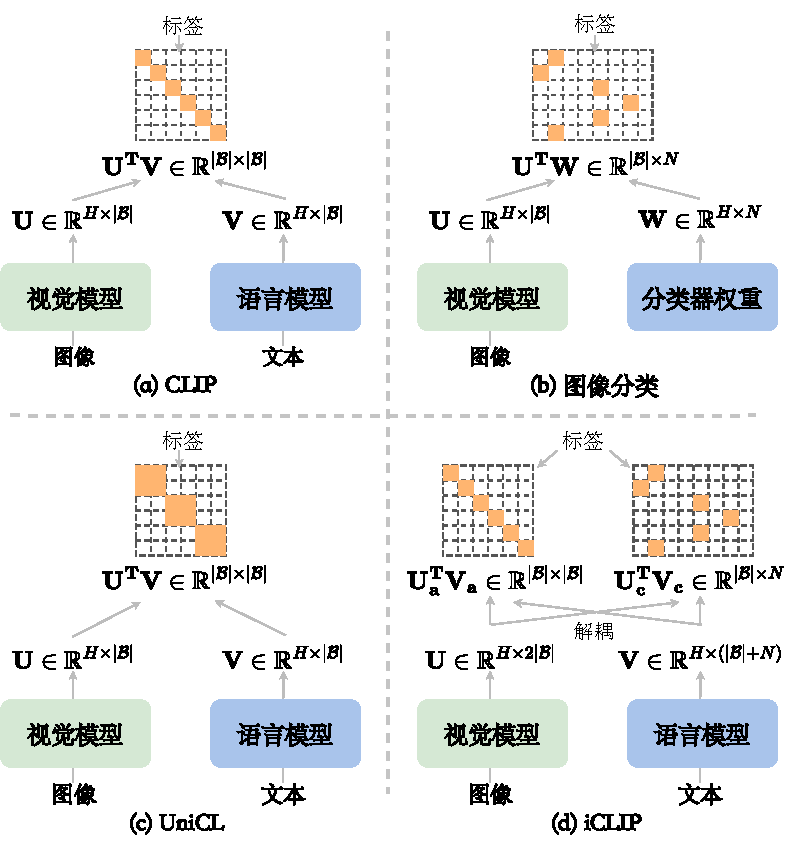
\includegraphics[width=0.8\linewidth]{figures/iclip-unicl.pdf}
  \caption{CLIP、图像分类、UniCL与本文iCLIP方法的对比图}
  \label{fig:iclip-unicl}
\end{figure}

\paragraph{与同期工作的比较} 
与本章工作同期也有一个工作UniCL\cite{unicl}采用了类似的想法:通过对比学习思想重新表达图像分类方法,从而与语言-图像对比学习方法进行有效融合,同样验证了本章介绍的基于高质量数据增强语言-图像对比学习预训练方法的有效性。
虽然两种方法具有相似的动机,但两者在方法设计上仍有两处较大区别,影响了方法融合程度和预训练效果。
% 对齐损失函数的基于余弦相似度的图像分类损失函数方法、对齐分类器类型的语言模型重参数化分类器权重方法、对齐标注语义丰富程度的外部专家知识库增强图像类别语义方法
首先,两种方法在如何融合两种预训练任务的设计上有区别。图\ref{fig:iclip-unicl}展示了CLIP方法、图像分类方法、UniCL方法与本节介绍的iCLIP方法的异同。
UniCL方法和iCLIP方法都在图像分类方法中引入了基于余弦相似度的损失函数和语言模型重参数化分类器权重方法,这使得两种数据集的标注信息,包括替代文本或图像类别,都可以通过共享的语言模型来建模,从而得以建立不同语义概念间的内部联系。

但两者在损失设计上并不相同。由于批大小的限制,同一批次内来自图像分类数据的图像只会覆盖全部$N$个图像类别中的一小部分。iCLIP方法会将这些图像与所有可能的类别名称进行对比学习,而UniCL方法只会将其与当前批次采样到的小部分类别名称进行对比学习,负样本对数量明显减小。
因此UniCL方法的损失设计很大程度上减小了图像分类数据可获取的训练信号,无法充分利用可区分性较高的图像分类标注信息。
% 此外,UniCL方法要求CLIP方法与图像分类的类别标签一起进行判别,由于替代文本语义涵盖更加丰富往往会涵盖类别名称,使得CLIP图文对的对比学习任务然而出现混淆情况。% 可能画个图可以说清楚
UniCL方法的损失设计优势在于无须设计并行训练架构。但如第\ref{sec:iclip-unify}节中所述,iCLIP方法提出了一个通过分布式计算的实现方案,可以将图像分类数据中涉及的所有类别均匀地分配给不同的并行模型实例,因此同样可以支持图像类别数较多的大规模图像分类数据的高效训练。%并在第\ref{sec:iclip-22k-laion}节中将其推广到亿级别的训练数据。

其次,两种方法的第二个主要区别在于iCLIP方法通过引入外部专家知识库,进一步缩小了图像类别的标签文本和图文对数据的替代文本间标注语义丰富度的差异。这种方法通过引入图像类别对应的额外语义信息,将类别标签文本扩展为内容更丰富的图像类别描述,提升了预训练视觉表征的语义丰富度,也提高了语言模型建模不同语义概念的能力。


\begin{table}
%\vspace{-0.5em}
    \centering
    % \addtolength{\tabcolsep}{-1.0pt}
    \caption{iCLIP方法与UniCL方法在图像识别能力上的对比实验}
    \begin{tabular}{lcccc}
    \toprule
        \multicolumn{1}{c}{} &
        \multicolumn{1}{c}{} & \multicolumn{1}{c}{} & \multicolumn{2}{c}{领域内和零样本开放集合图像识别任务} \\
        % \cmidrule(lr){1-1}
        % \cmidrule(lr){2-3}
        % \cmidrule(lr){4-5}
        \midrule
        序号 & 数据 & 方法 & IN-1K评测集(\%) & UniCL-14泛化评测集(\%)   \\
        % \cmidrule(lr){1-1}
        % \cmidrule(lr){2-3}
        % \cmidrule(lr){4-5}
        \midrule
        % ImageNet-1K &  Swin-Tiny \\
        \#1 & 数据组合一 & UniCL & 36.4 & 45.5 \\  
        \#2 & 数据组合一 & iCLIP & \textbf{45.9} & \textbf{49.9} \\  

        % \cmidrule(lr){1-1}
        % \cmidrule(lr){2-3}
        % \cmidrule(lr){4-5}
        \midrule
        
        \#3 & 数据组合二 & UniCL & 40.5 & 49.1 \\
        \#4 & 数据组合二 & iCLIP & \textbf{50.9} & \textbf{54.4} \\   

        % \cmidrule(lr){1-1}
        % \cmidrule(lr){2-3}
        % \cmidrule(lr){4-5}
        \midrule
        
        \#5 & 数据组合三 & UniCL & 70.5  & 52.4 \\
        \#6 & 数据组合三 & iCLIP & \textbf{76.3} & \textbf{55.5} \\

        \bottomrule
    \end{tabular}
    \label{tab:iclip-tounicl}
\end{table}

表\ref{tab:iclip-tounicl}展示了UniCL方法和iCLIP方法在IN-1K评测集和UniCL-14泛化评测集上的Top-1准确率,以对比两种方法在领域内和零样本开放集合图像识别任务上的表现。在三种不同的数据集组合设置下,iCLIP方法在IN-1K评测集上的Top-1准确率比UniCL方法至少高出5\%。具体而言,在数据组合三的实验中,由于预训练数据包含IN-1K图像类别,此时IN-1K评测集的结果反映了预训练方法的领域内图像识别能力。在该项任务上iCLIP方法仍明显优于UniCL方法,表明UniCL方法的损失设计并没有充分利用图像分类数据的训练信号。同时,在UniCL-14泛化评测集代表的零样本开放集合图像识别任务上,iCLIP方法也明显优于UniCL方法。实验结果表明,使用完整类别集合进行对比学习能够显著增强预训练视觉表征的判别能力。
% 同时在最大规模的IN-22K与YFCC-14M组合数据上,如实验序号\#6所示,iCLIP方法在泛化评测集上达到55.5\%的平均Top-1 准确率,比实验序号\#5的UniCL方法高3.1\%。
此外,表\ref{tab:iclip-tounicl-ret}中比较了UniCL方法和iCLIP方法在零样本图文跨模态检索任务上的性能,并展示了Flickr30K数据集和MSCOCO数据集上图像检索与文本检索任务的Top-1召回率。得益于第\ref{sec:iclip-adapt-external}节中提出的外部专家知识库增强图像类别语义做法,iCLIP方法在各个图文跨模态检索测试中均取得优于UniCL方法的表现。



\begin{table}
%\vspace{-0.5em}
    \centering
    % \addtolength{\tabcolsep}{-1.0pt}
    \caption{iCLIP方法与UniCL方法在图文跨模态检索能力上的对比实验}
    \begin{tabular}{lcccccc}
    \toprule
        \multicolumn{1}{c}{} &
        \multicolumn{1}{c}{} & \multicolumn{1}{c}{} & \multicolumn{4}{c}{零样本图文跨模态检索任务(\%)} \\
        % \cmidrule(lr){1-1}
        % \cmidrule(lr){2-3}
        % \cmidrule(lr){4-7}
        \midrule
        序号 & 数据 & 方法 & Flickr-IR & Flickr-TR & COCO-IR & COCO-TR    \\
        % \cmidrule(lr){1-1}
        % \cmidrule(lr){2-3}
        % \cmidrule(lr){4-7}
        \midrule
        % ImageNet-1K &  Swin-Tiny \\
        \#1 & 数据组合一 & UniCL & 21.5 & 37.9 & 12.5 & 21.2 \\  
        \#2 & 数据组合一 & iCLIP & \textbf{31.9} & \textbf{49.8} & \textbf{15.5} & \textbf{27.2} \\  

        % \cmidrule(lr){1-1}
        % \cmidrule(lr){2-3}
        % \cmidrule(lr){4-7}
        \midrule
        
        \#3 & 数据组合二 & UniCL & 34.0 & 50.3 & 17.7 & 28.0 \\
        \#4 & 数据组合二 & iCLIP & \textbf{37.1} & \textbf{55.7} & \textbf{18.5} & \textbf{30.7}\\   
        % \cmidrule(lr){1-1}
        % \cmidrule(lr){2-3}
        % \cmidrule(lr){4-7}
        
        % 5 & YFCC + IN-22K & UniCL~\cite{unicl} & -  & - & - & - \\
        % 6 & YFCC + IN-22K & iCLIP & 36.2 & 55.3 & 18.0 & 29.7 \\
        \bottomrule
    \end{tabular}

    \label{tab:iclip-tounicl-ret}
\end{table}


%$^\ddag$表示为本文复现结果。因为使用IN-22K与YFCC-14M组合数据训练的UniCL模型并未公开,这一数据组合在此任务上不进行汇报。


\begin{table}
  \centering
  % \addtolength{\tabcolsep}{-2.0pt}
    \caption{iCLIP方法与公开大规模语言-图像对比学习方法的对比实验}
    %IN-22K和Laion-400M数据组合上的消融研究。我们在 ImageNet 数据集 (IN-1K [8] 和 IN-S [56])上评测模型,并在 Kornblith-12 数据集基准 [27] 上评测零样本评测。在 Kornblith-12 数据集上进行了小样本学习和对三个下游任务的微调,以评测iCLIP的迁移能力。$^\ddag$表示使用公开的模型权重进行测试。}
  \begin{tabular}{lcccccc}
  % method | visual encoder arch | image numbers# | IN-1K | IN-S | 12-zero | 12-four-shot | ADE | LVIS | K400
    \toprule
    \multicolumn{1}{c}{} & \multicolumn{1}{c}{} & \multicolumn{1}{c}{} & \multicolumn{2}{c}{IN-1K评测集(\%)} &
    \multicolumn{2}{c}{Kornblith-12评测集(\%)} \\
    % \cmidrule(lr){1-1} \cmidrule(lr){2-2} \cmidrule(lr){3-3} \cmidrule(lr){4-5} \cmidrule(lr){6-7} 
    \midrule
    序号 & 方法 & 预训练数据 & IN-1K & IN-S & 零样本 & 少样本\\
    % \cmidrule(lr){1-1} \cmidrule(lr){2-2} \cmidrule(lr){3-3} \cmidrule(lr){4-5} \cmidrule(lr){6-7}
    \midrule
    \#1 & OpenAI CLIP & 私有数据 & 68.6 & 46.6 & 68.8 & 66.4 \\
    
    \#2 & OpenCLIP & Laion-400M & 67.1 & 52.4 & \textbf{70.9} & -\\ %86.1+91.7+71.4+50.2+69.4+83.7+17.7+82.9+50.8+89.3+91.7+66.6 = 801.3 + 50.2
 
    % \cmidrule(lr){1-1} \cmidrule(lr){2-2} \cmidrule(lr){3-3} \cmidrule(lr){4-5} \cmidrule(lr){6-7} 
    \midrule
    \#3 & 仅图像分类 & ImageNet全集 & 82.6 & 42.0 & - & 67.6 \\
    \#4 & 仅对比学习 & Laion-400M & 61.1 & 51.5 & 67.2 & 73.3 \\
    \multirow{2}{*}{\#5} & \multirow{2}{*}{iCLIP} & ImageNet全集 & \multirow{2}{*}{\textbf{82.9}} & \multirow{2}{*}{\textbf{59.8}} & \multirow{2}{*}{70.6} & \multirow{2}{*}{\textbf{78.1}} \\
    & & 和Laion-400M & & & & \\
    \bottomrule
  \end{tabular}

  \label{tab:iclip-overall-zeroshot}
\end{table}



\subsection{亿级图像规模的组合实验}
\label{sec:iclip-22k-laion}
本组实验使用最大规模的公开数据集对iCLIP方法进行验证,展示了在超大数据规模下高质量图像分类数据对语言-图像对比学习方法的提升效果,并与其他大规模方法的结果进行比较。除了对比不同方法在零样本开放集合图像识别任务上的表现,本节实验还在各类下游视觉任务中对预训练模型进行微调,比较了不同方法在图像语义分割、长尾类别物体检测和视频动作识别等任务上的迁移效果。

% $^\ddag$符号表示使用公开的模型权重进行测试
\paragraph{领域内和零样本开放集合图像识别任务评测结果} 表\ref{tab:iclip-overall-zeroshot}中展示了iCLIP方法与大规模语言-图像对比学习方法:OpenAI的CLIP\cite{radford2021learning}工作和OpenCLIP\cite{openclip}工作的评测对比结果,以及iCLIP方法与单预训练方法基线的对比结果。
% 对于单图像分类任务的基线,结果直接使用Swin-Base发布版本的结果,该模型在IN-22K上训练了90个轮次。对于单实例级语言监督任务的基线,结果来自在Laion-400M上预训练3个轮次的结果,因此该组实验使用的图片数目与单图像分类任务中使用的图片数目相当。
实验结果显示,iCLIP方法在IN-1K评测集上与单图像分类方法基线的结果相当,这表明两种方法在处理领域内图像识别任务时具有相当的性能。在IN-S评测集上,iCLIP方法比单图像分类方法基线提升了17.8\%的Top-1准确率,证明了iCLIP方法得到的视觉表征健壮性更强,对图像分布变化更稳定。与单语言-图像对比学习方法基线相比,iCLIP方法在Kornblith-12评测集上的开放集合图像识别任务表现提升了3.4\%的平均Top-1准确率。
与一些使用了私有数据或训练数据轮数更多的大规模语言-图像对比学习方法结果相比,iCLIP方法在IN-1K评测集上提升明显,主要是因为预训练数据中的ImageNet全集覆盖了IN-1K评测集中的图像类别。但是iCLIP方法在IN-S评测集上的结果也优于大规模语言-图像对比学习方法的结果,这表明iCLIP方法确实可以得到更健壮的视觉表征。
此外,iCLIP方法虽然预训练数据轮次较少,但是在Kornblith-12测试集上的平均Top-1准确率与OpenCLIP工作的结果相当,并优于使用私有数据的OpenAI CLIP\cite{radford2021learning}工作。 % 这也可能由于视觉模型结构有差异+Self pretrain


\begin{figure}
  \centering
  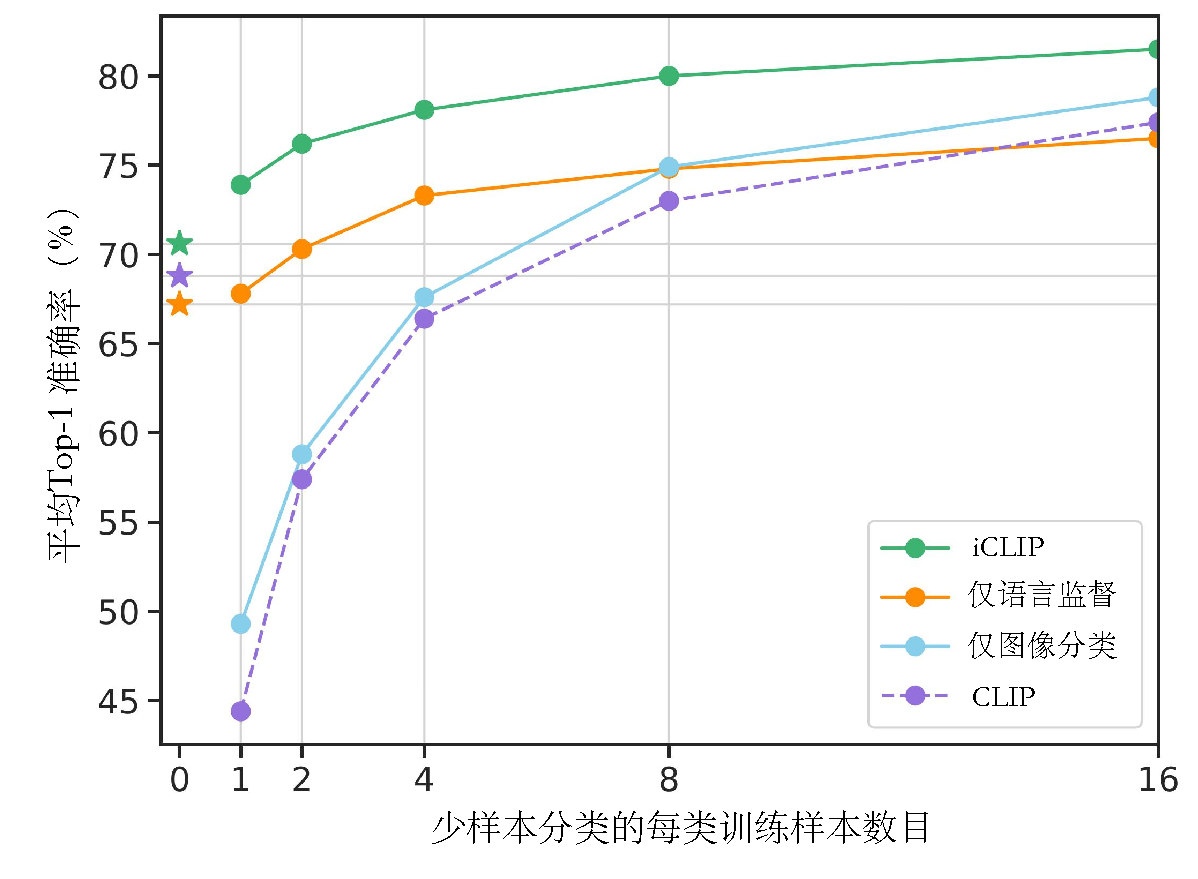
\includegraphics[width=0.8\linewidth]{figures/iclip-fewshot.pdf}
  \caption{iCLIP方法与不同方法在少样本图像识别任务微调上的性能比较}
  % todo: CLIP改为OpenAI CLIP
  % \todo{图4:与 Kornblith 12 数据集上小样本分类的 CLIP-ViT-B/16 的主要比较,展示了平均Top-1准确率。⋆表示零镜头性能。使用发布的模型再现了 CLIP 对少数镜头分类的结果。我们每个实验运行 3 次,并报告平均结果。}
  \label{fig:iclip-fewshot}
\end{figure}

\paragraph{少样本图像识别任务微调结果} 本组实验还比较了不同预训练方法在少样本图像识别任务上的微调性能,并选用Kornblith-12数据集作为训练和评测数据集。这项微调任务设置遵循了OpenAI CLIP工作的原始设置:在微调过程中固定视觉模型不变,只微调额外的类别分类器。
% 这组评测按照CLIP给出的设置实现:冻结视觉模型并增加一个额外的线性分类层以进行少样本微调。
如图\ref{fig:iclip-fewshot}所示,OpenAI CLIP工作在每个图像类别可训练样本数较少时的微调表现要弱于零样本图像识别任务评测结果,除非每个图像类别使用4个以上的训练样本。这是因为当少样本图像识别任务微调的训练样本数量有限时,随机初始化的类别分类器难以得到很好的训练,因此无法充分反映视觉表征中蕴含的语义信息。
基于前述利用对比学习方法重新表达图像分类任务的方法,在本组实验中直接微调经过预训练的语言模型作为类别分类器,而不是微调随机初始化的类别分类器。预训练过的语言模型能够为少样本图像识别任务微调提供良好的初始化,并缩小了语言-图像对比学习预训练阶段与少样本图像识别任务微调阶段之间的差异。

当每个图像类别只使用一个训练样本时,使用语言模型重参数化分类器权重的做法使得iCLIP方法达到73.9\%的平均Top-1准确率。相比于OpenAI CLIP工作高出29.5\%,也比iCLIP方法的零样本基线高出3.3\%,验证了其在少样本微调任务上的优势。当每个图像类别使用16个训练样本时,iCLIP方法的微调性能仍然比OpenAI CLIP工作要高4.1\%。
与单图像分类方法和单语言-图像对比学习方法的基线相比,iCLIP方法在单样本微调下的平均Top-1准确率分别提高了24.6\%和6.1\%,并在16个训练样本的设置中依然保持2.7\%和5.0\%的性能提升。

\begin{table}
  \centering
  % \addtolength{\tabcolsep}{-2.0pt}
    \caption{iCLIP方法与不同方法在下游视觉任务上的微调性能比较}
    %IN-22K和Laion-400M数据组合上的消融研究。我们在 ImageNet 数据集 (IN-1K [8] 和 IN-S [56])上评测模型,并在 Kornblith-12 数据集基准 [27] 上评测零样本评测。在 Kornblith-12 数据集上进行了小样本学习和对三个下游任务的微调,以评测iCLIP的迁移能力。$^\ddag$表示使用公开的模型权重进行测试。}
  \begin{tabular}{lccc}
  % method | visual encoder arch | image numbers# | IN-1K | IN-S | 12-zero | 12-four-shot | ADE | LVIS | K400
    \toprule
    \multicolumn{1}{c}{} & \multicolumn{1}{c}{图像语义分割} & \multicolumn{1}{c}{长尾类别物体检测} & \multicolumn{1}{c}{视频动作识别}\\
    % \cmidrule(lr){1-1} \cmidrule(lr){2-4}
    \midrule
  方法 & mIoU得分 & 检测框mAP得分 & Top-1准确率(\%)\\
    % \cmidrule(lr){1-1} \cmidrule(lr){2-4}
    \midrule
    仅图像分类方法 & 52.1 & 35.9 & 82.7 \\
    仅对比学习方法 & 52.0 & 36.6 & 82.3 \\
    iCLIP &\textbf{52.6} & \textbf{37.9} & \textbf{83.1} \\
    \bottomrule
  \end{tabular}

  \label{tab:iclip-overall-transfer}
\end{table}

\paragraph{在其他视觉下游任务上的微调结果} 本节对比了不同方法在其他视觉下游任务上的微调效果。如表\ref{tab:iclip-overall-transfer}所示,与仅使用图像分类方法的基线相比,iCLIP方法在图像语义分割、长尾类别物体检测和视频动作识别任务上分别提升了0.5的mIoU得分、2.0的检测框mAP得分和0.4\%的Top-1准确率。与仅使用对比学习方法的基线相比,iCLIP方法在三项视觉任务微调上也分别有0.6、1.3和0.8\%的提升。这些结果表明iCLIP方法获得的视觉表征具有更强的泛化能力。


\section{总结}
\label{sec:iclip-summary}
% 我们的贡献总结如下:
% ・我们将图像分类和对比语言 - 图像预训练这两个重要的视觉任务合并到一个框架中。
% ・我们发现原始图像分类公式可以适应 CLIP 方法,而性能几乎没有下降。根据这一发现,我们提出了一种有效融合方法,其中两个任务共享相同的文本编码器和相同的分类器类型,其有效性在基准测试中得到了广泛验证。
% ・我们提出了一种简单而有效的方法,将知识库引入图像分类中,解决了原始短图像名称的歧义和多义问题,并进一步弥合了类和替代文本之间的差距。它还首次展示了将知识库应用于计算机视觉问题。
% 背景+motivation
语言-图像对比学习方法通过对比学习框架在图文对数据中寻找正负样本对驱动模型预训练,并扩展到大规模互联网图文对数据。
但是这些图文对数据中存在大量标注噪声,影响了视觉表征与语言表征的对齐效果。

% 解决方案和发现
本章提出利用已有的人工标注数据,如高质量图像分类数据作为互联网图文对数据的补充。为有效融合两种不同形式的数据源和对应的训练方法,本章提出iCLIP预训练方法。
iCLIP方法一方面从语言-图像对比学习方法的角度重新理解传统的图像分类方法,统一了两种方法的损失函数形式和分类器参数化方式,另一方面引入外部专家知识库增强图像类别语义信息,对齐了不同数据在标注信息语义丰富度上的差异,并减少了类别标签间的歧义。
% 引入已有经过人工标注的数据源进行增强,一方面扩展了数据来源和监督信号类别,另一方面也提高了数据整体信噪比,有利于数据利用效率的提升。特别地,本章以已有的图像分类数据为主要对象,经过对图像分类任务的解析与重构,发现该类任务可以从实例级语言监督任务的角度重新诠释和建模,且不会损害其原有的学习效率,因此使得其有机会与原先的基于实例级对比的联合预训练方法,也即CLIP,进行有效融合。
% 具体来说,为将传统的图像分类任务与基于实例级对比的联合预训练方法对齐,引入了三项调整内容:用余弦相似度统一损失函数,用语言模型统一监督信号建模,引入外部知识哭缩小标签信息粒度差距。
经过高质量图像分类数据增强后的语言-图像对比学习iCLIP方法在零样本开放集合图像识别任务和图文跨模态检索任务上取得明显性能提升,并在亿级图像的大规模训练数据上得到验证。
% 同时本章工作在三种不同的数据组合规模,从百万级到亿级图片上进行了验证,充分展示了该方法的数据可扩展性。

% 引入下一章
虽然iCLIP方法在语义分割、物体检测等下游视觉任务上的微调性能有所提升,但提升幅度相对有限。因此,下一章将深入研究语言-图像对比学习方法在细粒度视觉任务上的迁移任务,并提出相应的改进方案。
% !TeX root = ../main.tex
\chapter{基于特征图自蒸馏增强的细粒度视觉任务迁移方法}
\label{cha:fd}

“预训练-微调”是计算机视觉领域基于深度学习的重要范式,深刻影响了领域内一系列重要工作\cite{HinSal06,alexnet,rcnn13,long2015fully}。第\ref{cha:iclip}章中讨论的图像分类预训练方法是最常用的预训练方法之一,亦可用于增强语言-图像对比学习方法视觉表征的语义建模能力,提高模型在零样本开放集合图像识别和图文跨模态检索任务上的表现。然而,与不依赖语义信息的像素级自监督预训练方法\cite{he2022masked}相比,CLIP方法在细粒度视觉任务上的迁移表现欠佳。虽然第\ref{cha:iclip}章中介绍的iCLIP方法显著改善了视觉-语言表征的对齐效果,但其在下游视觉任务上的迁移性能提升有限。因此,充分发挥CLIP方法的语义表征优势,增强其在下游视觉任务上的迁移性能,并实现对像素级自监督预训练方法的性能超越是本章的研究目标。

% 通过这种有监督预训练方法得到的模型权重,是各种下游视觉任务微调阶段的初始化权重。


\section{引言}
\label{sec:fd-intro}

CLIP方法通过海量互联网图文数据对进行预训练,一方面解决了图像分类方法对高质量人工标注数据的依赖,另一方面将图像标注的语义信息从固定集合的单一类别标签扩展为内容丰富、语义多样的自然语言描述。因此,CLIP方法的视觉模型展现出强大的语义建模能力,在固定视觉模型的线性探测分类任务上可以取得优异的表现。%在开放集合图像识别任务和图文跨模态检索任务上表现优异。
% 解决了图像分类低噪声有标注数据获取难和有限标签限制监督信号语义信息两大难题,因而可以扩展到利用互联网级规模的数据进行预训练,并展现出令人印象深刻的语义建模能力,从而逐步代替了以图像分类任务为代表的有监督预训练方法。
% 关于这一点,第\ref{cha:iclip}章在零样本或少样本图像识别任务和图文检索任务上进行了充分的性能分析,但实验结果也反映出了CLIP方法相比于图像分类方法在下游视觉任务上的迁移表现,并没有取得和其在图像识别或图文检索任务中一致的明显性能提升。iCLIP方法在CLIP方法基础上引入低噪声的图像分类数据,也并未观察到在下游视觉任务迁移性能上的显著改进。

与CLIP方法的思路相反,自监督预训练方法不以利用语义信号为主要目标,而是从图像数据自身寻找结构信息和监督信号。受自然语言处理领域的掩码语言模型\cite{BERT}相关工作启发,基于掩码图像模型\cite{bao2021beit, xie2022simmim, he2022masked}的自监督预训练方法要求模型通过给定的部分图像输入,预测被掩码区域的图像内容,从而在视觉模型预训练中引入像素级训练信号。这种像素级自监督方法可扩展性良好,在各类下游视觉任务中展现出优异的迁移性能,已经成为最重要的自监督预训练方法之一。本章主要讨论其中的代表性工作MAE\cite{he2022masked}。与像素级自监督方法相比,CLIP方法的视觉模型在许多下游视觉任务,尤其是依赖密集感知能力的细粒度视觉任务上并无优势。这一现象与理论预期存在明显矛盾:线性探测分类任务性能直接反映了CLIP方法视觉表征的语义表达能力,而具有更丰富语义信息的视觉表征理应在下游任务中获得更好的性能表现。
% \todo{可能需要一个MAE v.s. CLIP的图?要不然都不知道MAE是什么}

% 比较两种不同的预训练方法可以发现,语言-图像对比学习方法利用大规模图文数据对学习了丰富的语义信息,因此在固定视觉模型的线性探测分类任务上可以取得非常优异的表现。然而,相比于像素级自监督方法,语言-图像对比学习方法得到的视觉模型在许多下游视觉任务,尤其是依赖密集感知能力的细粒度视觉任务上的迁移性能并无优势。这种现象看似矛盾:线性探测性能反映了视觉表征的表达能力,而具有更丰富语义信息的表征理应在下游任务中表现更好。

% 特别地,前期实验发现,在细粒度视觉任务上相比于MIM方法表现甚至更弱。
% 因此这就提出了一个进一步的问题:CLIP方法得到的视觉模型能否在下游视觉任务,尤其是细粒度视觉任务微调方面取得与MIM方法一样的效果,甚至超越MIM方法得到的视觉模型?

针对这一问题,本章提出像素级训练信号对于提升预训练模型在下游细粒度视觉任务上的迁移性能具有关键作用。%\cite{xie2021propagate} 发展历史上实例级自监督任务与像素级自监督任务的对比,
% 为了验证这两项因素分别对实例级语言监督预训练方法CLIP的模型迁移能力的影响,需要在现有方法中引入相应设计。尽管对齐输入完整性的差异相对简单,但要将CLIP的训练目标的粒度从实例级扩展到像素级是一个重大挑战,因为这种方案不符合大规模互联网数据的基本形态,(图像,替代文本)对往往只反映实例级的对应信息,缺乏对细粒度关系的标注。
然而,CLIP作为一种基于实例级对比学习的方法,仅建模了图像全局表征与文本全局表征之间的对齐关系。由于互联网图文数据对仅提供实例级别的对齐信号,与像素级对齐所需的细粒度标注存在根本冲突,因此将CLIP方法的训练目标从实例级扩展到像素级是一个重大挑战。%,(图像,替代文本)对往往只反映实例级的对应信息,缺乏对细粒度关系的标注。
尽管已有研究(如局部化叙事\cite{LocNar})提出了一些更高效的数据标注方法以引入像素级图文对齐的标注信息,但这类方法的数据标注成本仍然较高,难以获取大规模数据。这一局限性使其与CLIP方法依赖海量图文数据对的设计理念存在冲突。
% 违背了以CLIP为例预训练方法的重要出发点。

为了解决像素级训练信号缺失的问题,同时避免大规模像素级数据标注成本,本章研究并借鉴了一项传统方法:知识蒸馏\cite{hinton2015knowledge}。知识蒸馏是一种将训练好的模型(教师模型)的知识转移到待训练模型(学生模型)中的方法。因此知识蒸馏方法常被用于模型压缩场景,即将参数量较大的教师模型的知识转移到参数量较小的学生模型中,从而达到节约应用成本的目的。
% 从广义上说,人工标注数据驱动的深度学习方法也是一种知识蒸馏方法。这一过程中人类被视作教师模型,而神经网络被视为学生模型。
而知识蒸馏方法的核心思想,是通过教师模型将具有复杂结构信息的输入数据转化为更明确且易于学习的训练信号,用于驱动学生模型训练。

本章提出知识蒸馏方法可以作为一种训练信号的转换机制,不需要额外的数据标注即可在CLIP方法中引入像素级训练目标。同时,这种方法不用重新进行昂贵的预训练,既保留了教师模型蕴含的语义信息,又提升了学生模型在下游视觉任务上的迁移表现。具体而言,本章提出了一种称为特征图自蒸馏的知识蒸馏方法,简称为FD方法。特征图自蒸馏方法以通过CLIP方法预训练好的模型作为教师模型。在不失一般性的前提下,本章使用最常用的OpenAI CLIP\cite{radford2021learning}模型作为教师模型。给定任一图像,该方法先用权重固定的CLIP模型提取图像对应的输出特征图,再将这些特征图作为蒸馏目标,训练一个随机初始化的、与教师模型参数量相同的学生模型,最终将其迁移至下游视觉任务中。
% 整个过程如图\ref{fig:fd-overall}所示,输入图像的黄色框代表对原始图像进行随机裁剪的数据增强方法,输出特征图中的橙色块对应着描述了图像全局信息的特殊标记[\texttt{CLS}]。
% 特征图自蒸馏方法与传统的未归一化概率知识蒸馏的方法\cite{hinton2015knowledge,deit}不同。一方面前者采用特征图作为蒸馏信号,而后者采用模型输出的类别未归一化概率作为蒸馏信号,另一方面前者以引入像素级训练目标为主要目的,需要尽可能保留教师模型能力,因此使用参数量一致的学生模型,而后者则主要被用于模型压缩场景,常使用参数量小得多的学生模型。

此外,本章还提出在蒸馏过程中引入一些适当的归纳偏置和正则化,以进一步提升学生模型在下游视觉任务上的迁移性能。本章设计了以下改进措施:1)对教师模型的特征图进行标准化,放大特征图中的细微信息,并稳定训练信号的值域,便于蒸馏阶段的超参数调整;2)在教师模型和学生模型之间使用不对称比例的随机深度,减少学生模型过拟合风险,增强视觉表征的鲁棒性,同时确保教师模型产生稳定且准确的蒸馏信号;3)引入层间共享的相对位置偏置,帮助学生模型学习视觉表征的平移不变特性。

% 以CLIP模型为教师模型,并应用前述特征图自蒸馏方法得到一个新的学生模型,称为FD-CLIP模型。
基于前述的特征图自蒸馏方法,本章以CLIP模型为教师模型,训练得到了一个学生模型,并将其命名为FD-CLIP。该模型在保留了教师模型语义信息的同时,在下游视觉任务上展现出更优异的迁移性能。与原始CLIP模型相比,FD-CLIP模型在各种视觉任务上均取得明显改进:在图像分类任务中,Top-1准确率提高了2.1\%;在语义分割任务中,mIoU得分提高了2.2;在目标检测和实例分割任务中,检测框mAP和分割掩码mAP得分分别提高了3.2和2.7;在深度估计任务中,均方根误差(RMSE)降低了0.064。使用更大尺寸的CLIP模型作为教师模型时,对应的FD-CLIP模型在ImageNet-1K数据集上取得89.0\%的Top-1准确率,超过了一些使用10倍预训练数据的方法。此外,本章发现特征图自蒸馏方法还可以应用于其他非CLIP方法预训练的模型,例如实例级自监督模型DINO\cite{dino}、图像分类有监督模型DeiT\cite{deit}和有三十亿参数的大规模视觉模型SwinV2-G\cite{swinv2cvpr}。特征图自蒸馏之后,这些模型在各种下游任务迁移中取得一致的性能提升。特别地,经过特征图自蒸馏的FD-SwinV2-G模型在MSCOCO数据集\cite{chen2015microsoft}的目标检测任务上取得了64.2的检测框mAP,刷新了当时该任务的记录。

FD-CLIP模型在下游任务上的优异迁移性能表明,尽管其学习自教师模型,但像素级训练目标的引入可能赋予了学生模型与教师模型不同的、有益于下游任务迁移性能的特征属性\cite{xie2023revealing}。为了验证这一假设并深入理解特征图自蒸馏方法的工作机制,本章引入了多种模型特征属性诊断工具来分析不同方法间的模型差异。通过这些诊断工具,本章发现具有像素级训练目标的掩码图像模型展现出了一系列优异的特征属性,而经过特征图自蒸馏的FD-CLIP模型表现出类似的性质。这些分析为理解特征图自蒸馏方法如何改进下游视觉任务的迁移性能提供了更深入的见解。具体而言,特征图自蒸馏后的CLIP模型具有如下性质:1)增加了较深的层中不同注意力头的感受野多样性;2)增强了视觉表征的平移不变特性;3)使下游任务的损失景观平坦化,增加迁移过程的稳定性。

综上所述,本章的主要内容安排如下:
\begin{itemize}
    \item 第\ref{sec:fd-intro}节指出了CLIP方法在下游细粒度视觉任务上的欠佳表现,介绍了通过特征图自蒸馏引入像素级训练信号的方案,并提出利用模型特征属性诊断工具分析自蒸馏前后模型的行为差异。
    \item 第\ref{sec:fd-method}节介绍了本章的研究方法,包括特征图自蒸馏方法具体做法、蒸馏过程中的归纳偏置和正则化方法设计以及各类模型特征属性诊断工具的可视化方式与主要目的。
% 包括从对比学习角度理解图像分类任务的具体设计以及引入外部专家知识库对类别语义进行增强的具体方法等,并提出深度融合的统一预训练方法iCLIP的具体形式。
    \item 第\ref{sec:fd-result}节介绍了本章的实验设置、评测指标和模型在各类下游任务的迁移实验,以及各模块的消融分析,并给出特征图自蒸馏方法在其他模型上应用的实验结果。
    \item 第\ref{sec:fd-summary}节对本章内容进行了总结。
\end{itemize}

\section{研究方法}
\label{sec:fd-method}

\subsection{语言-图像对比学习方法与掩码图像模型对比}
\begin{figure}
  \centering
  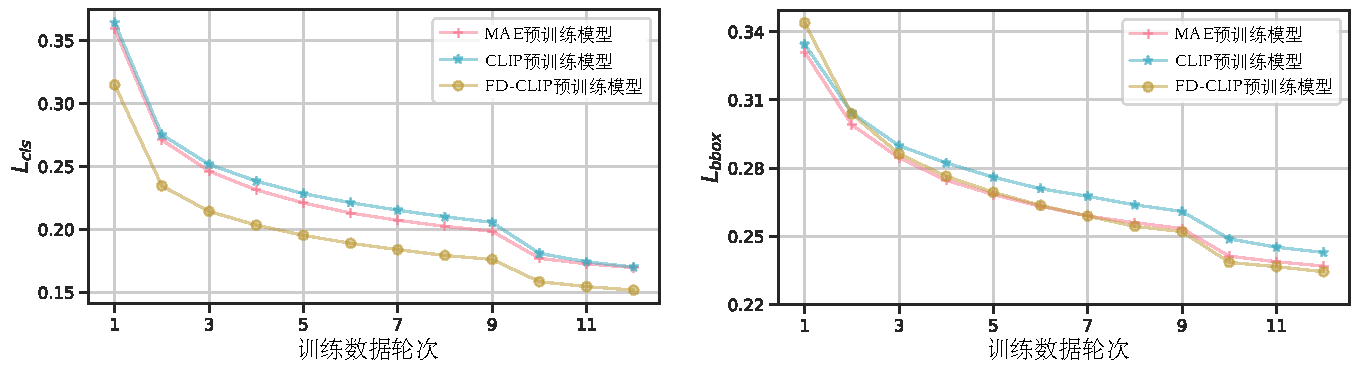
\includegraphics[width=1.0\linewidth]{figures/fd-coco-abl.pdf}
  \caption{MAE、CLIP和FD-CLIP模型在目标检测任务上的损失曲线对比}
    % \todo{图2:在 MSCOCO 对象检测任务上微调 MAE、CLIP 和 FD-CLIP。我们可视化了 $L_{cls}$ 和 $L_{bbox}$ 相对于训练时期的损失曲线。虽然 CLIP 预训练与 $L_{cls}$ 的 MAE 预训练相当,但它显示出更差的定位能力,反映在 $L_{bbox}$ 曲线上。}
    % 还有一个lvis的,可以画在ablation里
  \label{fig:fd-coco-abl}
\end{figure}

% 语言-图像对比学习方法能整合通过对比巨大的图像文本对学到的丰富语义而闻名,与MIM方法(例如MAE)相比,CLIP方法得到的视觉模型与人类概念联系更紧密。然而,它令人印象深刻的语义能力似乎对下游任务微调的好处帮助有限。

本节首先分析了CLIP方法和MAE方法在MSCOCO\cite{chen2015microsoft}数据集目标检测任务上的表现。
目标检测任务主要包含目标定位与物体识别两个任务\cite{ren2016faster}。前者属于需要密集感知能力的细粒度任务,而后者则属于对语义能力要求较高的实例级任务,因此可以用于观察不同预训练方法的视觉模型在两种不同任务上的行为表现。
图\ref{fig:fd-coco-abl}中展示了不同预训练模型在MSCOCO数据集上的训练损失曲线。在物体识别训练损失$L_{cls}$上,MAE方法和CLIP方法之间的表现非常接近,但MAE方法预训练的模型具有更好的细粒度感知能力,因此其目标定位损失$L_{bbox}$相较于CLIP方法得到的模型更低。
这些差异促使本章进一步研究影响CLIP方法迁移性能的关键因素,以更好地释放其预训练中掌握的语义信息,同时增强其处理细粒度视觉任务的能力。

\begin{table}
\caption{
不同预训练方法的输入完整性、训练目标粒度和损失函数设计表格}
% ,除了MAE方法之外,BEiT也是一个典型的像素级自监督预训练方法。
\centering
  \begin{tabular}{lcccc}
    \toprule
  方法 & 输入完整性 & 训练目标粒度 & 损失函数设计 & 是否使用语义信息 \\
  \midrule
  BEiT & 部分图像 & 像素级任务 & 交叉熵损失函数 & \\ 
  MAE & 部分图像 & 像素级任务 & 回归损失函数 & \\
  % SimMIM~\cite{xie2021simmim}? & partial? & token-level & regression & \\ % if we mentioned them, we need to put it in table1?
  \midrule
  CLIP & 完整图像 & 实例级任务 & 交叉熵损失函数 & $\checkmark$  \\
  % 新方法 & Full & Token-level & \color{gray}{Regression} & $\checkmark$ \\
\bottomrule
  \end{tabular}
\label{tab:fd-differences}
\end{table}

% 要回答这个问题,本章首先将这些预训练方法的要素分解为三个方面:输入完整性、训练目标粒度和损失函数设计。
% 如表\ref{tab:fd-differences}所示,通过比较CLIP与两种典型MIM方法之间的设计要素差异,可以排除了损失函数设计为主要影响因素,并推测输入完整性(是否使用对完整图像还是部分图像进行建模)和训练目标粒度(是实例级监督任务还是像素级监督任务)是可能因素。
% 结合自监督预训练任务发展历史上实例级自监督任务与像素级自监督任务的对比\cite{xie2021propagate},像素级训练目标粒度的设计可能对模型在下游任务的迁移效果以及在细粒度视觉任务上的表现起到关键因素。
% 为了验证这两项因素分别对实例级语言监督预训练方法CLIP的模型迁移能力的影响,需要在现有方法中引入相应设计。尽管对齐输入完整性的差异相对简单,但要将CLIP的训练目标的粒度从实例级扩展到像素级是一个重大挑战,因为这种方案不符合大规模互联网数据的基本形态,(图像,替代文本)对往往只反映实例级的对应信息,缺乏对细粒度关系的标注。
% 尽管有一些工作如局部化叙事\cite{LocNar}(Localized Narratives)提出了一些新的相对高效的数据标注方法来引入像素级对齐的信息,但这样的方法的数据可扩展性还是很低,违背了以CLIP为例预训练方法的重要出发点。

为进一步分析,本节将不同预训练方法的核心要素分解为三个方面:输入完整性、训练目标粒度和损失函数设计。表\ref{tab:fd-differences}中展示了CLIP方法和两个典型的掩码图像模型:MAE与BEiT\cite{bao2021beit}方法之间的设计差异。对比MAE与BEiT方法可以看到,两种掩码图像模型分别使用了回归损失函数和交叉熵损失函数,因此可以排除损失函数设计对细粒度视觉任务性能的影响。基于上述分析,本节考虑对齐掩码图像模型,使用与其一致的输入完整性和训练目标粒度设计来增强CLIP方法在下游视觉任务中的迁移性能。
% 并推测输入完整性(是否使用对完整图像还是部分图像进行建模)和训练目标粒度(是实例级监督任务还是像素级监督任务)是可能因素。
% :输入完整性、训练目标粒度和损失函数设计,本节考虑对齐MIM方法设计中使用的输入完整性和训练目标粒度来增强CLIP模型的迁移性能。
在这两个方面中,虽然使用部分图像作为CLIP方法的输入相对容易\cite{FLIP},但因为大规模获取图像像素与文本内容细粒度对齐的图文数据对非常困难,所以将CLIP方法的训练目标粒度从实例级扩展到像素级仍是一个重大挑战。此外,CLIP方法的预训练成本较高。以OpenAI CLIP模型为例,其预训练过程中使用超过4亿张训练图片和数百张显卡训练数周,才能达到较好效果。因此,本节方法旨在避免重新预训练且不依赖额外数据标注的前提下,实现在CLIP方法中引入部分图像的输入设计和像素级的训练目标粒度设计。

\subsection{特征图自蒸馏方法}

\begin{figure}
  \centering
  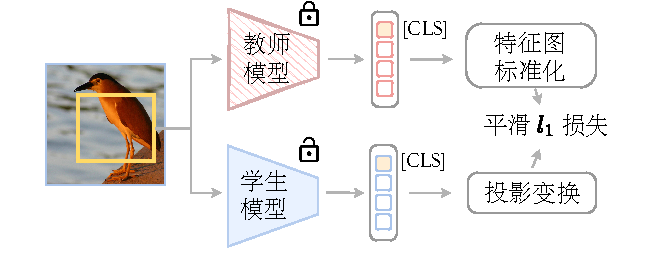
\includegraphics[width=0.8\linewidth]{figures/fd-overall.pdf}
  \caption{利用特征图自蒸馏方法引入像素级训练信号的流程图}
  % \todo{图 1:特征图蒸馏图,引入令牌级目标来蒸馏预训练的 CLIP 模型。橙色块代表 [\texttt{CLS}] 令牌,橙色框表示原始图像的随机裁剪。}
  \label{fig:fd-overall}
\end{figure}

% 整个过程如图\ref{fig:fd-overall}所示,输入图像的黄色框代表对原始图像进行随机裁剪的数据增强方法,输出特征图中的橙色块对应着描述了图像全局信息的特殊标记[\texttt{CLS}]。

% 特征图自蒸馏方法与传统的未归一化概率知识蒸馏的方法\cite{hinton2015knowledge,deit}不同。一方面前者采用特征图作为蒸馏信号,而后者采用模型输出的类别未归一化概率作为蒸馏信号,另一方面前者以引入像素级训练目标为主要目的,需要尽可能保留教师模型能力,因此使用参数量一致的学生模型,而后者则主要被用于模型压缩场景,常使用参数量小得多的学生模型。

受知识蒸馏方法启发,本节提出利用知识蒸馏作为训练目标转换方法,将CLIP方法的训练目标粒度从实例级扩展到像素级,同时最大程度保留预训练CLIP模型的语义信息。
整个特征图自蒸馏过程如图\ref{fig:fd-overall}所示。输入图像的黄色框代表对原始图像进行随机裁剪的数据增强方法,输出特征图中的橙色块对应着描述了图像全局信息的特殊标记[\texttt{CLS}]。
和传统知识蒸馏方法类似,特征图自蒸馏方法使用预训练好的CLIP模型充当教师模型并固定参数不动,同时随机初始化一个新模型作为学生模型,来尽可能保留教师模型预训练过程中建模的语义信息。%,同时在此阶段引入像素级任务以增强视觉模型在细粒度任务上的迁移表现。

和传统知识蒸馏方法不同,特征图自蒸馏方法有如下两个特征:
\begin{itemize}
    \item 采用预训练模型的完整输出特征图作为蒸馏目标,而不是以未归一化概率为蒸馏目标\cite{hinton2015knowledge,deit}。该做法一方面可以引入像素级训练目标,并为学生模型提供更多可蒸馏信号以尽可能保留教师模型的能力。另一方面,因为很多预训练模型\cite{dino}并没有未归一化概率的输出形式,该做法也使得特征图自蒸馏方法可以运用到更多预训练模型中。
    此外,为了确保特征图逐像素对齐,特征图自蒸馏方法需要对输入教师模型和学生模型的图像应用相同的图像增强方法。
    后续实验表明,与蒸馏其他实例级特征相比,蒸馏整个特征图可以更显著地增强CLIP方法在下游视觉任务的迁移效果,验证了之前关于像素级训练目标对模型细粒度视觉任务迁移效果重要性的猜想。
    \item 使用相同大小的教师模型和学生模型,而不是大参数的教师模型和小参数的学生模型。这种做法的原因是特征图自蒸馏方法并非为了压缩模型,而是为了在引入像素级训练目标的同时,尽可能使得学生模型保留教师模型中蕴含的语义信息和视觉能力。
    虽然学生模型的训练目标是尽可能模仿教师模型的输出特征图,但从随机初始化开始训练允许学生模型有不同的优化路径。这种优化路径上的差异为学生模型提供了具备与掩码图像模型相似特征属性的可能性。
\end{itemize}

% \begin{figure}
%   \centering
%   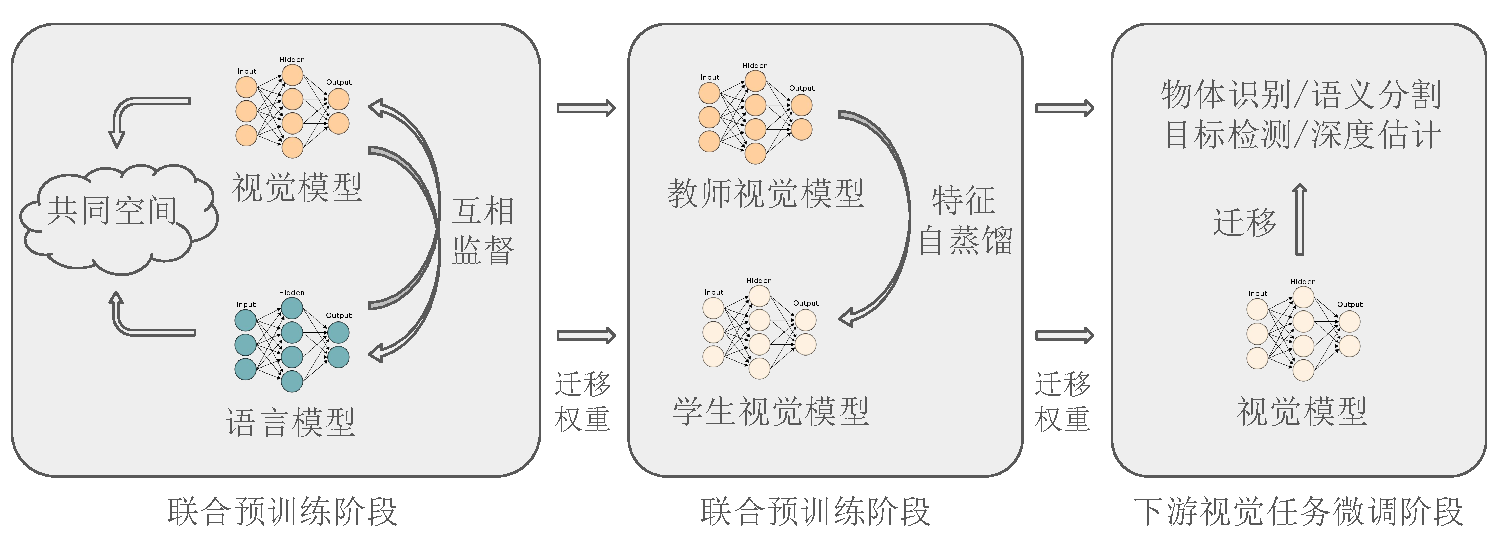
\includegraphics[width=1.0\linewidth]{figures/fd-framework-update.pdf}
%   \caption{新引入的“特征图自蒸馏”阶段在整个“预训练-微调”范式中的作用}
%     % \todo{图2:在 MSCOCO 对象检测任务上微调 MAE、CLIP 和 FD-CLIP。我们可视化了 $L_{cls}$ 和 $L_{bbox}$ 相对于训练时期的损失曲线。虽然 CLIP 预训练与 $L_{cls}$ 的 MAE 预训练相当,但它显示出更差的定位能力,反映在 $L_{bbox}$ 曲线上。}
%   \label{fig:fd-framework-update}
% \end{figure}

\begin{table}
\caption{特征图自蒸馏方法的输入完整性、训练目标粒度和损失函数设计表格}
\centering
  \begin{tabular}{lcccc}
\toprule
  方法 & 输入完整性 & 训练目标粒度 & 损失函数设计 & 是否带语义信息 \\
  \midrule
  MAE & 部分图像 & 像素级任务 & 回归损失函数 & \\
  % SimMIM~\cite{xie2021simmim}? & partial? & token-level & regression & \\ % if we mentioned them, we need to put it in table1?
  \midrule
  CLIP & 完整图像 & 实例级任务 & 交叉熵损失函数 & $\checkmark$  \\
  FD-CLIP & 完整图像 & 像素级任务 & 回归损失函数 & $\checkmark$ \\
\bottomrule
  \end{tabular}
\label{tab:fd-method}
\end{table}

% 因此,该方法称作“特征图自蒸馏”方法,因其使用的蒸馏目标是特征图,教师模型是它自身。
如表\ref{tab:fd-method}所示,通过以上设计,特征图自蒸馏方法得以在保留预训练CLIP模型语义信息的同时,不需要额外数据标注即可引入像素级训练信号,从而达到以较小的代价增强CLIP方法在下游视觉任务迁移性能的目的。% 新引入的“特征图自蒸馏”方法在整个“预训练-微调”范式中xxx。该阶段在不重新预训练CLIP模型的前提下,以较小的成本引入像素级监督任务,可以理解为是针对预训练模型的一次“中间训练”(Mid-training)。

\subsection{归纳偏置和正则化方法设计}
基于特征图自蒸馏方法的双分支结构,本节提出在蒸馏过程中引入额外的归纳偏置和正则化方法,以进一步提升学生模型在下游视觉任务上的迁移性能。
% 接着,在“特征图自蒸馏”方法基础上,本节设计并引入以下归纳偏置和正则化策略,以进一步提高学生模型的迁移效果。
\paragraph{对教师模型的输出特征图进行标准化} 不同预训练模型的输出特征图有各自的数值范围,直接回归这些特征图使得蒸馏过程中需要针对不同模型调整超参数,限制了方法的通用性。此外,一些特征图中的细节信息被编码在相对小的数值中。如果不对这些细微信号进行放大,学生模型在蒸馏过程中往往会忽略这些信息。为了解决这些问题,本节提出使用标准化操作对教师网络的输出特征图进行后处理,使得不同输出特征图的均值为0,方差为1。% https://ssjcoding.github.io/2019/03/27/normalization-and-standardization/
该操作可通过无参数的层归一化\cite{ba2016layer}实现。接着,特征图自蒸馏方法在学生和教师模型特征图之间采用平滑$\ell_{1}$损失函数进行监督,以减少离异特征值的影响。% https://blog.csdn.net/ai_faker/article/details/117414614
以$s$和$t$分别表示学生和教师模型的输出特征图,特征图自蒸馏方法公式化如下:
\begin{equation}
    \mathcal{L} (s, t) = \begin{cases}
        \frac{1}{2} (g(s) - t')^2/\beta, & | g(s) - t' | \leq \beta \\
        |g(s)-t'|-\frac{1}{2}\beta, & | g(s) - t' | > \beta,
    \end{cases}
    \label{eq:iclip-distill}
\end{equation}
其中$\beta$值设为2,而$t'$表示对教师输出特征图$t$进行标准化后的特征图。$g$是单个线性层,实现轻量级的投影变换以允许教师和学生模型之间有不同的输出特征图维度,从而增强了该方法的通用性。在CLIP方法训练过程中,视觉模型通过特殊标记[\texttt{CLS}]聚合图像全局信息并与语言表征进行对齐,因此[\texttt{CLS}]标记相比于特征图中的其他位置蕴含了更丰富的语义信息。考虑到这一点,在特征图自蒸馏方法中,[\texttt{CLS}]标记对应的蒸馏损失权重为其他位置的10倍,从而增强学生模型保留教师模型语义信息的效果。

\paragraph{不对称比例的随机深度} 特征图自蒸馏方法的双分支结构允许在教师模型和学生模型上应用不对称的正则化强度。实验发现,这种策略可以使学生模型在下游视觉任务的迁移性能更佳。具体来说,特征图自蒸馏过程中会在学生模型分支上添加一定比例的随机深度正则化\cite{huang2016deep},而在教师模型分支上不添加任何正则化。这种设计既保证了教师模型蒸馏信号的稳定性,不对学生模型的训练造成干扰,又减轻了学生模型的过拟合风险。

\paragraph{层间共享的相对位置偏置} 预训练的CLIP模型采用绝对位置编码策略,也即通过对不同位置的输入标记使用不同的索引来进行区分。最近的工作\cite{Swin,li2022mvitv2}发现相对位置偏置增强了视觉表征的平移不变性,因此对模型的迁移性能有一定好处。
由于特征图自蒸馏方法仅依赖于模型最后一层特征图,因此该方法可以灵活调整学生模型的位置编码策略。实验表明层间共享的相对位置偏置策略\cite{bao2021beit}能够提升模型的迁移性能。这种策略要求模型所有层使用相同的相对位置偏置矩阵,从而缓解深层网络中因为不同位置间特征相似性过高导致的表征坍缩的问题\cite{xie2023revealing}。% 实验表明,层间共享的相对位置偏置的总体性能最佳。
通过模型特征属性诊断工具可以发现使用这种位置编码策略使得模型不同注意力头的感受野更加多样化,允许模型建模更多不同位置的图像信息。这一现象在较深的模型层中更为明显。% (\todo{如补充材料中的图所示})

\subsection{模型特征属性的诊断工具}
为进一步理解特征图自蒸馏前后模型行为的变化,本节引入多个特征属性诊断工具对不同的模型进行对比分析,以提供对特征图自蒸馏方法背后机制的直观理解:
\begin{itemize}
    \item 注意力头级别的诊断工具:平均注意力距离\cite{dosovitskiy2020vit,xie2023revealing}。本章使用的视觉模型结构为Vision Transformer\cite{dosovitskiy2020vit}(ViT)。该模型结构中的自注意力层建模了不同像素位置间的相关关系,而每个自注意力层包含多个自注意力头用于建模不同的像素间关系。平均注意力距离的诊断工具统计了每个像素与其他像素间经过注意力权重加权后的相对距离的平均值,因此反映了每个自注意力头的感受野范围大小。在统计过程中,由于特殊标记[\texttt{CLS}]不包含任何位置信息,因此不会纳入统计范围。
    \item 模型层级别的诊断工具:平均注意力图\cite{zhou2021deepvit}。通过平均所有注意力头的注意力图可以得到层级别的平均注意力图。注意力图中有两种常见的模式:对角线模式和竖线模式。对角线模式表明该模型更多地依赖于来自相对位置关系的视觉线索,具有更好的视觉表征平移不变性,这是对各种下游视觉任务迁移性能的有益属性。同时,越是靠近中心对角线的对角线模式越能反映出模型学到了一些基于图像连续性的局部先验。而竖线模式则表明处于某些固定位置的图像输入对所有其他位置的特征产生了较大影响,这种模式反映了模型提取的视觉表征往往是平移变化的,抗干扰能力较弱。
    \item 模型级别的诊断工具:归一化的损失景观\cite{li2018visualizing}。这一诊断工具通过对迁移后的模型权重施加一系列不同程度的高斯噪声进行扰动,并观察扰动后的模型性能变化。噪声强度根据每个权重的$\ell_2$范数来决定,以消除不同模型权重幅度不同的影响。通常而言,损失局部极小值附近损失景观越平坦,则模型的优化过程更稳定、泛化性能更佳\cite{li2018visualizing}。
\end{itemize}

\section{实验结果}
\label{sec:fd-result}

% 本节展示了在已经训好的CLIP模型基础之上引入特征图自蒸馏阶段对下游任务迁移性能的提升情况,并对该方法的一些关键设计、推广性和诊断性质进行了深入分析。
第\ref{sec:fd-exp-setting}节介绍了特征图自蒸馏阶段和后续视觉任务迁移的实验设置。第\ref{sec:fd-exp-clip}节中展示了特征图自蒸馏后的CLIP模型在各类下游视觉任务的性能提升情况,并在第\ref{sec:fd-exp-input}节讨论了输入图像完整性和不同训练目标粒度的影响。第\ref{sec:fd-exp-detail}节包含归纳偏置和正则化方法对于模型迁移性能影响的消融实验,并在第\ref{sec:fd-more-models}节展示了将特征图自蒸馏方法应用到其他预训练模型后对下游任务迁移性能的提升情况。
最后,在第\ref{sec:fd-analysis}节中运用模型特征属性的诊断工具对蒸馏前后的模型进行了分析,以深入理解该方法特性。

\subsection{实验设置}
\label{sec:fd-exp-setting}
\paragraph{蒸馏阶段实验设置} 所有实验均使用ImageNet-1K\cite{deng2009imagenet}训练图像进行特征图自蒸馏。特征图自蒸馏方法以教师模型的输出特征图为监督目标,不依赖图像类别等人工标注信息,因此也可以在别的图像数据集上进行应用。除非特别说明,所有实验都在ImageNet-1K数据集(IN-1K)上蒸馏了100轮,并默认使用ViT-Base\cite{dosovitskiy2020vit}结构的CLIP模型(CLIP-Base)进行实验。%\todo{其他详细信息在补充材料中。}
\paragraph{迁移阶段实验设置} 为充分评测模型在各类下游视觉任务上的迁移效果,本节选择了4个下游任务:ImageNet-1K数据集\cite{deng2009imagenet}上的图像分类任务、ADE20K数据集\cite{zhou2019ade}上的语义分割任务、MSCOCO数据集\cite{chen2015microsoft}上的目标检测和实例分割任务以及NYUv2\cite{NYUv2}数据集上的深度估计任务。除图像分类任务外,其余三项任务均为细粒度视觉任务。各任务的具体设置如下:
\begin{itemize}
    \item \textbf{图像分类任务}~~ 该任务的迁移方法按照BEiT方法\cite{bao2021beit}的设置,使用AdamW优化器\cite{adamw}、逐层衰减的学习率和$224 \times 224$的输入图像分辨率。CLIP-Base模型在该任务上迁移100轮,而使用ViT-Large结构的CLIP模型(CLIP-Large)则迁移50轮。线性探测分类任务迁移实验则按照MAE方法的设置,使用LARS优化器\cite{lars}和0.1的学习率训练90轮,并将权重衰减设置为0。该任务使用ImageNet-1K评测集上的Top-1准确率进行报告。
    \item \textbf{语义分割任务}~~  该任务按照Swin方法\cite{Swin}中的描述,使用常用的UPerNet框架\cite{xiao2018upernet}进行迁移。迁移时使用AdamW优化器,以32的批大小训练8万个数据批次。其他超参数设置:学习率为4e-4、学习率逐层衰减强度为0.65、权重衰减为0.05、随机深度比例为0.2。在训练中,输入图像分辨率设置为$512 \times 512$。该任务使用单尺度输入进行测试并报告模型在验证集上的mIoU得分。
    \item \textbf{目标检测和实例分割任务}~~  该任务迁移阶段采用常见方法\cite{cae}的设置,包括使用MaskRCNN框架\cite{Mask-rcnn}在MSCOCO数据集上训练12轮,并使用多尺度训练和单尺度测试策略。为了降低全局自注意力层在高分辨率图像上的训练代价和内存开销,在该任务迁移时采用了滑动窗口注意力机制\cite{Swin},并将窗口的像素大小设置为$224 \times 224$,使其与预训练和蒸馏阶段中使用的图像尺寸一致。为了聚合图像的全局信息,在模型最后添加了一个额外的全局自注意力层。其他超参数设置如下:迁移过程中的批大小为16、最大学习率为2e-4、学习率逐层衰减系数为0.75,并遵循惯例,在第9和第11轮将学习率降低至先前的0.1倍。该任务使用模型在开发集上的检测框mAP和分割掩码mAP得分进行报告。
    \item \textbf{深度估计任务}~~  该任务的迁移阶段采用已有工作\cite{glpdepth, xie2023revealing}的设置,使用其中的24000张图像作为训练集迁移25轮,并在包含654张图像的官方测试集上进行评测,涵盖了215个不同室内场景的深度估计任务。其他超参数设置如下:输入图像被随机裁剪为$480 \times 480$的分辨率、迁移过程中的批大小为24、学习率为5e-5。该任务在测试时平均了两个方形窗口的预测结果,并使用模型在评测集上的均方根误差(RMSE)进行报告。
\end{itemize}

\paragraph{蒸馏阶段和迁移阶段的超参数设置}
表\ref{tab:fd-hyper-pretrain}中详细描述了蒸馏阶段和图像分类任务迁移阶段的超参数设置。

\begin{table}
    \centering
    \caption{特征图自蒸馏方法在蒸馏阶段和迁移阶段的超参数设置}
    \begin{tabular}{lcccc}
    \toprule
        & \multicolumn{2}{c}{蒸馏阶段} & \multicolumn{2}{c}{迁移阶段} \\
        \bf 超参数名称 & \bf CLIP-Base & \bf CLIP-Large & \bf CLIP-Base & \bf CLIP-Large \\
        \midrule
            图像块大小 & $16 \times 16$ & $14 \times 14$ & $16 \times 16$ & $14 \times 14$ \\
            层数  & 12 & 24 & 12 & 24\\
            隐变量维度 & 768 & 1024 & 768 & 1024\\
            前馈层中间维度 & 3072 & 4096 & 3072 & 4096 \\
            注意力头数目 & 12 & 16 & 12 & 16 \\
            注意力头宽度 & 64 & 64 & 64 & 64 \\
        \midrule
            训练轮数 & 300 & 300 & 100 & 50 \\
            批大小 & 2048 & 2048 & 2048 & 2048  \\
            输入图像分辨率 & $224 \times 224$& $224 \times 224$& $224 \times 224$& $224 \times 224$\\
            优化器参数$(\epsilon)$ & 1e-8 & 1e-8 & 1e-8 & 1e-8  \\
            优化器参数$(\beta)$ & (0.9,0.999)& (0.9,0.999)& (0.9,0.999)& (0.9,0.999)  \\
            最大学习率 & 1.2e-3 & 1.2e-3 & \{5e-3,6e-3\} & 1e-3  \\
            最小学习率 & 2e-5 & 2e-5 & 2e-6 & 2e-6 \\
            学习率调度形式 & 余弦调度 & 余弦调度 & 余弦调度 & 余弦调度 \\
            学习率热启动轮 & 10 & 10 & 20 & 5 \\
            学习率衰减系数 & 1.0 & 1.0 & \{0.6,0.65\} & 0.75 \\
        \midrule
            梯度截断系数 & 3.0 & 3.0 & 5.0 & 5.0 \\
            % Dropout & \multicolumn{4}{c}{\xmark} \\
            权重衰减系数 & 0.05 & 0.05 & 0.05 & 0.05\\
            随机深度比例 & 0.1 & 0.3 & \{0.1,0.2,0.3\} & 0.4 \\
            标签平滑比例 & - & - & 0.1 & 0.1 \\
            % 数据增强方法 & \multicolumn{2}{c}{随机缩放裁剪} & \multicolumn{2}{c}{ }\\
            % 这个列起来好长啊。。。
        \bottomrule
    \end{tabular}
    \label{tab:fd-hyper-pretrain}
\end{table}

\subsection{特征图自蒸馏后的CLIP模型迁移效果}
\label{sec:fd-exp-clip}
\paragraph{特征图自蒸馏后的CLIP-Base模型迁移效果} 本节首先在CLIP-Base模型上进行特征图自蒸馏实验,并将训练轮数扩展到300轮以充分验证结果。表\ref{tab:fd-clip_FD}展示了特征图自蒸馏后的模型在各类下游视觉任务上的迁移表现。
经过特征图自蒸馏得到的FD-CLIP模型在各类下游视觉任务上都有一定的性能提升,并在一些细粒度视觉任务上提升更为显著。相比于原始CLIP模型,FD-CLIP模型在ImageNet-1K图像分类任务上提高2.1\%的Top-1准确率,在语义分割任务上提高了2.2的mIoU得分,并在目标检测和实例分割任务上分别将检测框mAP和分割掩码mAP得分提高了3.2和2.7。此外,FD-CLIP模型在深度估计任务上也取得了明显的提升,均方根误差从0.416降低到了0.352。与此同时,FD-CLIP模型在各类下游视觉任务上的迁移表现已经超过了掩码图像模型MAE方法,验证了特征图自蒸馏能够显著提升CLIP方法在下游视觉任务上的迁移性能。

\begin{table}
\caption{特征图自蒸馏方法提升CLIP-Base模型的视觉任务迁移性能结果
% 该模型是在 ImageNet-1K 数据集 [10] 上提炼的,其中的图像只有 300 个 epoch。在四个评估基准上观察到明显的进步。MAE [17] 结果也以灰色列出以供参考。
}
\centering
% \addtolength{\tabcolsep}{-3.0pt}
% \renewcommand{\arraystretch}{1.1}
  \begin{tabular}{lccccc}
\toprule
   & IN-1K & ADE20K & \multicolumn{2}{c}{MSCOCO} & NYUv2 \\
   % \cline{2-3} \cline{5-6}
   \midrule
   % {AP$_\text{box}$} & {AP$_\text{mask}$}
方法    &   Top-1准确率 &  mIoU  & 检测框mAP & 分割掩码mAP & RMSE\scriptsize{ ($\downarrow$)}\\
  \midrule
  MAE & 83.6 & 48.1 & 46.5 & 40.9 & 0.383 \\

  \midrule
  
  CLIP & 82.9  & 49.5 & 45.0 & 39.8 & 0.416 \\
  FD-CLIP & 85.0  & 51.7 & 48.2 & 42.5 & 0.352 \\
  $\Delta$ & \textbf{$\uparrow$2.1}  &  \textbf{$\uparrow$2.2} & \textbf{$\uparrow$3.2} & \textbf{$\uparrow$2.7} & \textbf{$\downarrow$0.064}\\
\bottomrule
  \end{tabular}
\label{tab:fd-clip_FD}
\end{table}

% 在其他Validation set上的评测,表示鲁棒性
% To further evaluate the robustness of our model, we include more adversarial validation sets. Our FD-CLIP reaches 75.0\% and 43.8\% top-1 accuracy on ImageNet-v2 and ImageNet-sketch, higher than the original CLIP by \textbf{2.5\%} and \textbf{10.6\%}, respectively. These results show our method is not overfitted on ImageNet-1k validation set.

\begin{table}
\caption{特征图自蒸馏后的模型在零样本和线性探测分类任务上的表现
% \yx{Put init weight to appendix.} [这个啥意思来着?]
}
% \vspace{-0.3em}
\centering
% \addtolength{\tabcolsep}{-1.5pt}
% \renewcommand{\arraystretch}{1.1}
  \begin{tabular}{lccc}
\toprule
  评测方法 & CLIP & FD-CLIP & $\Delta$ \\
  \midrule
  零样本图像分类任务 (Top-1准确率) & 68.6 & 68.0 & -0.6 \\
  线性探测图像分类任务 (Top-1准确率) & 79.5 & 80.1 & +0.6 \\ 
\bottomrule
  \end{tabular}
\label{tab:fd-zero_shot}
\end{table}

\paragraph{特征图自蒸馏后的模型对预训练语义信息的保留情况} 
尽管特征图自蒸馏方法的训练目标与原始CLIP方法的训练目标不同,但由于蒸馏过程中学生模型充分学习了教师模型特征图,因此学生模型保留了大部分语义信息。
表\ref{tab:fd-zero_shot}比较了蒸馏前后的教师模型与学生模型在ImageNet-1K评测集上零样本和线性探测图像分类任务的Top-1准确率。结果表明蒸馏后的学生模型保留了原始CLIP模型蕴含的大部分语义信息。
% 也就是说,基于完整特征图的特征图自蒸馏方法可以在很大程度上保留了CLIP模型中包含的大量语义信息,同时可以取得优于MIM方法的迁移性能。

\paragraph{特征图自蒸馏方法的额外训练代价} 前述特征图自蒸馏方法使用ImageNet-1k数据集训练了300轮,而ImageNet-1K数据集包含128万张图像,因此总训练图像数目约为3.84亿张。OpenAI CLIP模型在预训练阶段使用私有的WIT-400M图文数据集\cite{radford2021learning}训练了32轮,因此总训练图像数目约为128亿张。由于语言模型参数量远小于视觉模型,此处忽略其预训练成本。
因此,特征图自蒸馏方法无需重新预训练或额外数据标注,通过3\%的额外训练成本,即可在各类下游视觉任务上带来大幅度性能提升。
% 这个代价是可以接受的,而且该方法不需要对CLIP进行重新训练,也不需要引入额外的数据标注代价。
此外,CLIP预训练过程依赖大量显卡才能达到足够的批大小:OpenAI CLIP模型需要256张以上显卡同时训练,而特征图自蒸馏方法对硬件要求较低,应用更为灵活。%对大多数实验室和团队都更友好。
% 原始的CLIP模型使用32768 的批大小和256个GPU进行训练,与CLIP预训练不同,特征图自蒸馏方法仅需要更小的批大小(2048),且只需要8个GPU即可训练,这对大多数实验室和团队都更友好。


\begin{table}
\caption{
特征图自蒸馏方法提升CLIP-Large模型的视觉任务迁移性能结果
% 扩展特征图自蒸馏方法至CLIP-Large模型后在图像任务上的迁移性能
}
\centering
% \addtolength{\tabcolsep}{-1.0pt}
% \renewcommand{\arraystretch}{1.1}
  \begin{tabular}{lccc}
\toprule
 方法 & 图像分辨率 & 训练数据集 & IN-1K Top-1准确率 \\
  \midrule
    WiSE-FT~\cite{ftclip2021} & 336$^2$ & WIT-400M~\cite{radford2021learning} & 87.1 \\
    DeiT III~\cite{touvron2022deit} & 384$^2$ & IN-22K~\cite{deng2009imagenet} & 87.7 \\
    ViT~\cite{dosovitskiy2020vit} & 512$^2$ & JFT-300M~\cite{Sun_2017_JFT300m} & 87.8 \\
   Scaling~\cite{zhai2022scaling} &  384$^2$ &  JFT-3B\cite{zhai2022scaling} &  88.5 \\
   BEiT~\cite{bao2021beit} &  512$^2$ &  DALLE~\cite{ramesh2021dalle1} \& IN-22K &  88.6 \\

  \midrule
  CLIP & $224^2$ & WIT-400M & 86.1 \\
  \midrule
  \multirow{3}{*}{FD-CLIP} & $224^2$ & WIT-400M & \textbf{87.7}\scriptsize{ (+1.6)} \\
   & 224$^2$ & WIT-400M \& IN-22K & \textbf{88.3}\scriptsize{ (+2.2)} \\
   & 336$^2$ & WIT-400M \& IN-22K & \textbf{89.0}\scriptsize{ (+2.9)} \\
\bottomrule
  \end{tabular}
\label{tab:fd-clip_large_FD}
\end{table}

\paragraph{特征图自蒸馏后的CLIP-Large模型迁移效果} 本组实验将特征图自蒸馏方法应用于CLIP-Large模型,以验证该方法的可扩展性。
如表\ref{tab:fd-clip_large_FD}所示,经过特征图自蒸馏的FD-CLIP模型在ImageNet-1K数据集图像分类任务中取得了87.7\%的Top-1准确率,相比原始CLIP模型提升1.6\%。
使用ImageNet-22K数据集迁移,并将图像分辨率扩展至$336\times 336$后,FD-CLIP模型在ImageNet-1K图像分类任务上取得了89.0\%的Top-1准确率,超过了使用接近10倍预训练数据方法\cite{zhai2022scaling}的性能表现。% 因为CLIP-Large模型使用14的块大小,并非2的整次幂,多分辨率的FPN与模型的块大小不兼容,因此没有在其他下游任务上进行微调比较。

\subsection{训练目标粒度和输入完整性对迁移性能的影响}
\label{sec:fd-exp-input}

\paragraph{训练目标粒度对迁移性能的影响} 本组实验研究了不同训练目标粒度对下游任务迁移性能的影响。本组实验比较了三种不同的训练目标粒度设置:
\begin{itemize}
    \item \textbf{蒸馏特殊标记特征}~~ 视觉模型中的[\texttt{CLS}]标记是一个特殊标记,并在CLIP方法中起到独特的作用:它不仅聚合了全局的图像信息,而且直接与语言表征进行对齐,因此蕴含了丰富的语义信息。在此设置中,蒸馏过程以教师模型的[\texttt{CLS}]标记输出特征作为训练目标构建了实例级训练目标粒度。
    \item \textbf{蒸馏全局平均特征}~~ 此设置是介于实例级训练目标粒度和像素级训练目标粒度的中间形式。具体来说,此设置对教师模型的输出特征图应用全局平均操作,以构造一个简化后的蒸馏目标。因此这个蒸馏目标同时包含了来自每个像素的特征信息,但又缺乏像素级的训练目标分辨率。
    \item \textbf{蒸馏完整特征图}~~ 这是特征图自蒸馏方法的默认设置,使用了教师模型的完整输出特征图作为蒸馏目标来构建像素级的训练目标粒度,并对[\texttt{CLS}]标记的对应特征使用更大的损失权重。
\end{itemize}

\begin{table}
\caption{自蒸馏过程中使用不同训练目标粒度的消融实验}
% 。这些模型是在 ImageNet-1K 数据集 [10] 上蒸馏的,有 100 个 epoch。代币级目标对于提高 CLIP 的迁移性能至关重要。
\centering
% \addtolength{\tabcolsep}{-2.5pt}
% \renewcommand{\arraystretch}{1.1}
  \begin{tabular}{lccccc}
\toprule
   & IN-1K & ADE20K & \multicolumn{2}{c}{MSCOCO} & NYUv2 \\
   % \cline{4-5}
   \midrule

   方法 &  Top-1准确率   &  mIoU  & 检测框mAP & 分割掩码mAP & RMSE\scriptsize{ ($\downarrow$)}\\
  \midrule

  MAE & 83.6 & 48.1 & 46.5 & 40.9 & 0.383 \\
    原始模型 & 82.9 & 49.5 & 45.0 & 39.8 & 0.416 \\ 
  % CLIP~\cite{radford2021learning} & 82.9 & 49.5 & 45.0 & 39.8 & 0.416 \\
  \midrule
  % FIXME: 这个要修-编译bug
  特殊标记特征 & 81.9 & 47.5 & 44.8 & 39.6 & 0.396 \\
  全局平均特征  & 83.3 & 50.3 & 46.3 & 40.6 & 0.393 \\
  完整特征图 & \textbf{84.4} & \textbf{51.8} & \textbf{47.9} & \textbf{42.2} & \textbf{0.350} \\
\bottomrule
  \end{tabular}
\label{tab:fd-ablation_targets}
\end{table}

表\ref{tab:fd-ablation_targets}展示了通过不同训练目标粒度蒸馏后的模型在下游任务上的迁移性能表现。蒸馏[\texttt{CLS}]标记特征的模型在深度估计任务上的误差有所减少,但在其他视觉任务上的性能相比原始CLIP模型没有提升,甚至有一定损失。这是因为[\texttt{CLS}]标记无法提供教师模型蕴含的全部信息。相比之下,蒸馏全局平均特征的模型在所有下游视觉任务中均展现出了一定的性能增益,但提升幅度微弱。蒸馏完整特征图的特征图自蒸馏方法引入了像素级训练目标粒度,相比于其他蒸馏目标而言,这一方法得到的模型在下游视觉任务中的迁移表现最佳,超过了MAE方法的迁移效果。结果表明像素级训练目标对提升CLIP方法的下游任务迁移性能至关重要。

\paragraph{输入完整性对迁移性能的影响} 这组实验研究了特征图自蒸馏方法中的输入完整性对下游视觉任务迁移性能的影响。为构造不同的输入图像比例,本组实验参考掩码图像模型,以块形状随机掩码部分图像后输入模型。%,比例分别设置为25\%、50\%、75\%和100\%(即完整图像)。
表\ref{tab:fd-ablation_masking}展示了对学生模型应用不同输入比例进行自蒸馏后在各类下游任务上的迁移性能,其中标注$^{\dag}$的实验表明教师模型的输入图像也缩减到对应比例,否则教师模型默认使用完整图像作为输入。

在相同的训练轮数下,使用完整图像和部分图像进行特征图自蒸馏得到的模型性能相近,但使用25\%输入比例设置的模型表现不佳。同时,教师模型的输入需要是完整图像,否则自蒸馏后的模型在一些深度估计等任务上的迁移表现欠佳。结果表明输入完整性不是影响CLIP方法在下游视觉任务上迁移效果的关键因素。
\begin{table}
\caption{自蒸馏过程中使用不同输入比例的消融实验
}
\centering
% \addtolength{\tabcolsep}{-1.5pt}
% \renewcommand{\arraystretch}{1.1}
  \begin{tabular}{lccccc}
\toprule
   & IN-1K & ADE20K & \multicolumn{2}{c}{MSCOCO} & NYUv2 \\
   % \cline{4-5}

   \midrule

   方法  &  Top-1准确率   &  mIoU  & 检测框mAP & 分割掩码mAP & RMSE\scriptsize{ ($\downarrow$)}\\
  \midrule

    MAE & 83.6 & 48.1 & 46.5 & 40.9 & 0.383 \\
    原始模型 & 82.9 & 49.5 & 45.0 & 39.8 & 0.416 \\ 
  % CLIP~\cite{radford2021learning} & 82.9 & 49.5 & 45.0 & 39.8 & 0.416 \\
\midrule
  $25\%$ 输入图像$^{\dag}$ & 83.3 & 47.8 & 45.2 & 40.1 & 0.397 \\
  $25\%$ 输入图像 & 83.1 & 48.8 & 45.1& 39.8& 0.379 \\
  $50\%$ 输入图像 & 84.2 & 51.5 & 47.5& 41.7& 0.351 \\
  $75\%$ 输入图像 & \textbf{84.4} & \textbf{52.0} & 47.8& 41.9 & \textbf{0.347} \\
  完整输入图像 & \textbf{84.4} & 51.8 & \textbf{47.9} & \textbf{42.2} & 0.350 \\
\bottomrule
  \end{tabular}
\label{tab:fd-ablation_masking}
\end{table}

\begin{table}
        \centering
        \caption{自蒸馏过程中使用部分比例输入图像并增加训练轮数的消融实验}
    \
        \begin{tabular}{lccccc}
            \toprule
               & 显卡 & IN-1K & ADE20K & MSCOCO & NYUv2 \\
               %\cline{5-6}
                \midrule
               方法 & 小时 &  Top-1准确率   &  mIoU  & 检测框mAP & RMSE\scriptsize{ ($\downarrow$)}\\
              \midrule
            %   100数据轮次 & 96.4 & 83.1 & 48.8 & 45.1& 39.8& 0.379 \\
            %   200数据轮次 & 192.8 & 83.9 & 49.7 & 46.4& 40.9& 0.366 \\
            %   400数据轮次 & 385.6 & \textbf{84.4} & 51.1 & 47.2& 41.5& 0.367 \\
            % %   $50\%$ + 100ep input & 84.2 & 51.5 & 47.5& 41.7& 0.351 \\
            % %   $50\%$ + 200ep input & 84.6 & 51.5 & 48.3& 42.3& 0.349 \\
            %   100数据轮次$^{\dag}$ & 170.7 & \textbf{84.4} & \textbf{51.8} & \textbf{47.9} & \textbf{42.2} & \textbf{0.350} \\
              100轮 & 96.4 & 83.1 & 48.8 & 45.1&  0.379 \\
              200轮 & 192.8 & 83.9 & 49.7 & 46.4& 0.366 \\
              400轮 & 385.6 & \textbf{84.4} & 51.1 & 47.2&  0.367 \\
            %   $50\%$ + 100ep input & 84.2 & 51.5 & 47.5& 41.7& 0.351 \\
            %   $50\%$ + 200ep input & 84.6 & 51.5 & 48.3& 42.3& 0.349 \\
              100轮$^{\dag}$ & 170.7 & \textbf{84.4} & \textbf{51.8} & \textbf{47.9} & \textbf{0.350} \\
            \bottomrule
        \end{tabular}
        \label{tab:fd-ablate_longer_maskinput}
\end{table}

考虑到使用25\%输入比例时,特征图自蒸馏方法的计算量相比于蒸馏完整输入图像时要更小,因此表\ref{tab:fd-ablate_longer_maskinput}研究了增加蒸馏训练轮数的影响,其中标注$^{\dag}$的实验代表蒸馏完整输入图像的实验基线。
实验结果表明,延长使用25\%输入比例的蒸馏数据至4倍训练轮数后,模型在细粒度视觉任务上迁移表现仍落后于蒸馏完整输入图像的默认设置。考虑到教师模型没法利用部分图像输入进行加速,此时实验设置需要的计算代价已经超过默认设置。因此使用完整输入图像进行蒸馏可以取得更优的迁移结果。
此外,表\ref{tab:fd-ablation_masking}的实验结果表明,使用75\%的输入比例进行特征图自蒸馏可以获得相近的迁移性能。此时对图像进行掩码可以被认为是一种数据增强方法,在减少过拟合风险的同时提供一定比例的加速效果。
% 综合以上实验可以得出结论:训练目标粒度对于提升下游视觉任务的迁移性能非常重要,输入完整性的影响不大。


\subsection{归纳偏置和正则化方法的消融}
\label{sec:fd-exp-detail}
本节讨论了特征图自蒸馏方法中不同归纳偏置和正则化方法设计对下游任务迁移性能的影响。本节实验对比了不同模型在ImageNet-1K图像分类任务上的迁移效果。

\begin{table}
    % \small
    \centering
    % \renewcommand{\arraystretch}{1.15}
    % \addtolength{\tabcolsep}{-3.5pt}
    \caption{
    特征图自蒸馏方法中归纳偏置和正则化方法的消融实验}
    \begin{tabular}{lccc}
        \toprule
        (a)特征图后处理设计 & 无 & $\ell_2$ 归一化 & 标准化 \\
        \midrule
        IN-1K (Top-1 准确率) & 83.5 & 83.9 & \textbf{84.4} \\
        \midrule
        (b)学生/教师的随机深度比例 & 0.1 / 0.1 & 0.1 / 0 & 0.2 / 0  \\
        \midrule
        IN-1K (Top-1 准确率) & 84.0 & \textbf{84.4} & 84.0 \\
        \midrule
        (c)位置编码设计 & 绝对位置编码 & 不共享相对编码 & 共享相对编码 \\
        \midrule
        IN-1K (Top-1 准确率) & 84.0 & 83.9 & \textbf{84.4} \\
        \bottomrule
    \end{tabular}
    \label{tab:fd-ablation_tricks}
\end{table}

\paragraph{不同教师特征图后处理方式的设计} 表\ref{tab:fd-ablation_tricks} (a)中对比了不同教师特征图后处理方式的效果。
与直接使用原始教师模型特征图作为蒸馏信号相比,教师模型特征图标准化带来了0.9\%的Top-1准确率提升。进一步对比$\ell_{2}$归一化方法和标准化方法,后者仍有0.5\%的增益。这种后处理方法使得特征图自蒸馏阶段的超参数对使用何种预训练模型不敏感,因此本章所有实验均采用标准化方式对教师模型的输出特征图进行后处理。

\paragraph{不对称比例随机深度的设计} 表\ref{tab:fd-ablation_tricks} (b)分析了不同程度的随机深度正则化的影响。实验表明在学生模型上适当使用一定比例的随机深度正则化对迁移性能有一定帮助,原因在于正则化减轻了蒸馏过程中过拟合的风险。但是,在教师模型上使用随机深度正则化对模型迁移性能有一定损害,这说明稳定的教师模型输出更有益。因此本章所有实验默认采用这种不对称比例随机深度的策略。

\paragraph{不同位置编码配置的设计} 表\ref{tab:fd-ablation_tricks} (c)探讨了学生模型使用不同位置编码配置后在下游任务上的迁移表现。结果表明,层间共享的相对位置编码配置优于其他位置编码配置。根据特征属性分析,这种位置编码配置可以使得模型具有更多样的图像感受野,增强了模型的表达能力。

\subsection{特征图自蒸馏方法增强其他预训练模型的迁移效果}
\label{sec:fd-more-models}


\begin{table}
\caption{
特征图自蒸馏方法提升DINO和DeiT模型的视觉任务迁移性能结果
% 这些模型是在 ImageNet-1K 数据集 [10] 上蒸馏的,并训练300个数据轮次。
}
\centering
% \addtolength{\tabcolsep}{-1.5pt}
% \renewcommand{\arraystretch}{1.1}
  \begin{tabular}{lccccc}
\toprule
   & IN-1K & ADE20K & \multicolumn{2}{c}{MSCOCO} & NYUv2 \\
   \midrule
方法    &  Top-1准确率   &  mIoU  & 检测框mAP & 分割掩码mAP & RMSE\scriptsize{ ($\downarrow$)}\\
  \midrule
  DINO & 82.8 & 46.2 & 45.8 & 40.7 & 0.412 \\
  FD-DINO & 83.8 & 47.7 & 46.1 & 40.9 & 0.394 \\
  $\Delta$ & \textbf{$\uparrow$1.0} & \textbf{$\uparrow$1.5} & \textbf{$\uparrow$0.3} & \textbf{$\uparrow$0.2} & \textbf{$\downarrow$0.018} \\
  \midrule
  
  DeiT & 81.8 & 47.0 & 45.8 & 40.7 & 0.403 \\
  FD-DeiT & 83.0 & 48.0 & 46.4 & 41.0 & 0.404 \\
  $\Delta$ & \textbf{$\uparrow$1.2} & \textbf{$\uparrow$1.0} & \textbf{$\uparrow$0.6} & \textbf{$\uparrow$0.3} & \textbf{$\uparrow$0.001} \\
\bottomrule
  \end{tabular}
\label{tab:fd-extend_dino_deit}
% \vspace{-1.0em}
\end{table}

\begin{table}
        \centering
    \caption{
特征图自蒸馏方法提升MAE模型的视觉任务迁移性能结果
}
        \begin{tabular}{lccccc}
            \toprule
               & IN-1K & ADE20K & \multicolumn{2}{c}{MSCOCO} & NYUv2 \\
               \midrule
              方法 &  Top-1准确率   &  mIoU  & 检测框mAP & 分割掩码mAP & RMSE\scriptsize{ ($\downarrow$)}\\
              \midrule
              MAE & 83.6 & 48.1 & 46.5 & 40.9 & 0.383 \\
              FD-MAE & 83.4 & 47.9 & 46.7 & 41.2 & 0.364 \\
              $\Delta$ & \textbf{$\downarrow$0.2} & \textbf{$\downarrow$0.2} & \textbf{$\uparrow$0.2} & \textbf{$\uparrow$0.3} & \textbf{$\downarrow$0.019} \\
            \bottomrule
        \end{tabular}
        \label{tab:fd-extend_mae}
\end{table}

表\ref{tab:fd-clip_FD}和表\ref{tab:fd-clip_large_FD}中展示的实验结果证明了在CLIP模型上应用特征图自蒸馏方法,可以有效改进其在下游视觉任务上的迁移表现。虽然本章工作主要针对CLIP模型,但本节实验验证了特征图自蒸馏方法对其他预训练模型的作用,从而进一步考察了该方法的通用性。
表\ref{tab:fd-extend_dino_deit}展示了在实例级自监督方法的DINO模型\cite{dino}和图像分类有监督方法的DeiT模型\cite{deit}上应用特征图自蒸馏方法后,模型在各类下游视觉任务迁移性能上的改进。
DINO模型和DeiT模型在预训练过程中均未引入带有像素级训练目标的视觉任务,因此其性质上与CLIP方法有一定的相似性。
实验结果表明,特征图自蒸馏方法对这些预训练方法的模型也有一定帮助,尤其提升了它们在语义分割和目标检测任务上的表现,但对它们在深度估计任务上的好处并不普遍。

虽然MAE方法在预训练阶段已经包括了像素级的视觉训练目标,但仍然可以对其应用特征图自蒸馏方法,并观察特征图自蒸馏方法对下游视觉任务性能的影响。表\ref{tab:fd-extend_mae}展示了以MAE模型为教师模型进行特征图自蒸馏方法后得到的模型在下游任务上的迁移结果。
实验结果表明FD-MAE模型在大多数视觉任务上的迁移表现与蒸馏前的教师模型的表现类似,仅在深度估计任务上有一定改进。%,但不如在CLIP方法上应用特征图自蒸馏后的改进明显。
这一结果验证了本章假设,即特征图自蒸馏方法的主要收益来自于低成本地引入像素级训练目标,因此掩码图像模型无法继续从特征图自蒸馏方法中获益。

\begin{table}
\caption{
特征图自蒸馏方法提升SwinV2-G模型的视觉任务迁移性能结果}
\centering
% \addtolength{\tabcolsep}{-3.5pt}
% \renewcommand{\arraystretch}{1.1}
  \begin{tabular}{lcccc}
  
\toprule

   &  IN-1K & \multicolumn{2}{c}{MSCOCO}  & ADE20K  \\
  \midrule
  方法 &Top-1 准确率 & 检测框mAP & 分割掩码mAP & mIoU \\
  \midrule
  GLIPv2-CoSwin-H~\cite{GLIPv2_2022} & - & 62.4 & - & - \\
  Florence-CoSwin-H~\cite{yuan2021florence} & - & 62.4 & - & -  \\
  DINO-Swin-L~\cite{zhang2022dino} & - & 63.3 & - & - \\
  MaskDINO-Swin-L~\cite{li2022mask} & - & - & 54.7 & 60.8 \\
  ViT-Adapter-L~\cite{chen2022vitadapter} & - & - & - & 60.5 \\
    
\midrule
  SwinV2-G & 89.2 & 63.1 & 54.4 & 59.9 \\
  FD-SwinV2-G & \textbf{89.4}\scriptsize{ (+0.2)} & \textbf{64.2}\scriptsize{ (+1.1)} & \textbf{55.4}\scriptsize{ (+1.0)} & \textbf{61.4}\scriptsize{ (+1.5)} \\
%      
  
\bottomrule
  \end{tabular}
\label{tab:fd-swinv2_G}
\end{table}

此外,为了进一步验证特征图自蒸馏方法的模型可扩展性,本组实验选用超大规模的SwinV2-G\cite{swinv2cvpr}模型进行实验。相比于前述使用的最大模型CLIP-Large,SwinV2-G模型含有超过三十亿个模型参数,模型规模扩大了10倍。
如表\ref{tab:fd-swinv2_G}所示,经过特征图自蒸馏的FD-SwinV2-G模型在ADE20K数据集的语义分割任务和MSCOCO数据集的目标检测任务上实现了61.4 mIoU得分和64.2 检测框mAP得分,相比于原先的最好方法MaskDINO-Swin-L和DINO-Swin-L\cite{zhang2022dino,li2022mask}分别提升了0.6和0.9。
FD-SwinV2-G模型与原始SwinV2-G模型使用相同的语义分割和目标检测迁移框架\cite{xiao2018upernet, chen2019htc},并保持评测设置不变,但相比于原始SwinV2-G模型,FD-SwinV2-G模型在目标检测和实例分割任务上继续取得超过1.0的mAP得分提升,并在语义分割任务上提升1.5的mIOU得分。
结果表明,特征图自蒸馏方法具有良好的通用性,可适用于不同预训练方法、网络结构和模型规模,提升它们在下游视觉任务上的迁移性能。


\subsection{模型特征属性分析}
\label{sec:fd-analysis}

本节使用第\ref{sec:fd-method}节介绍的模型特征属性诊断工具对蒸馏前后的CLIP模型进行分析,同时与掩码图像模型MAE方法进行对比,以进一步揭示特征图自蒸馏方法如何影响了模型特征属性。本节分析均使用ImageNet-1K评测集的图像。
\begin{figure}
  \centering
  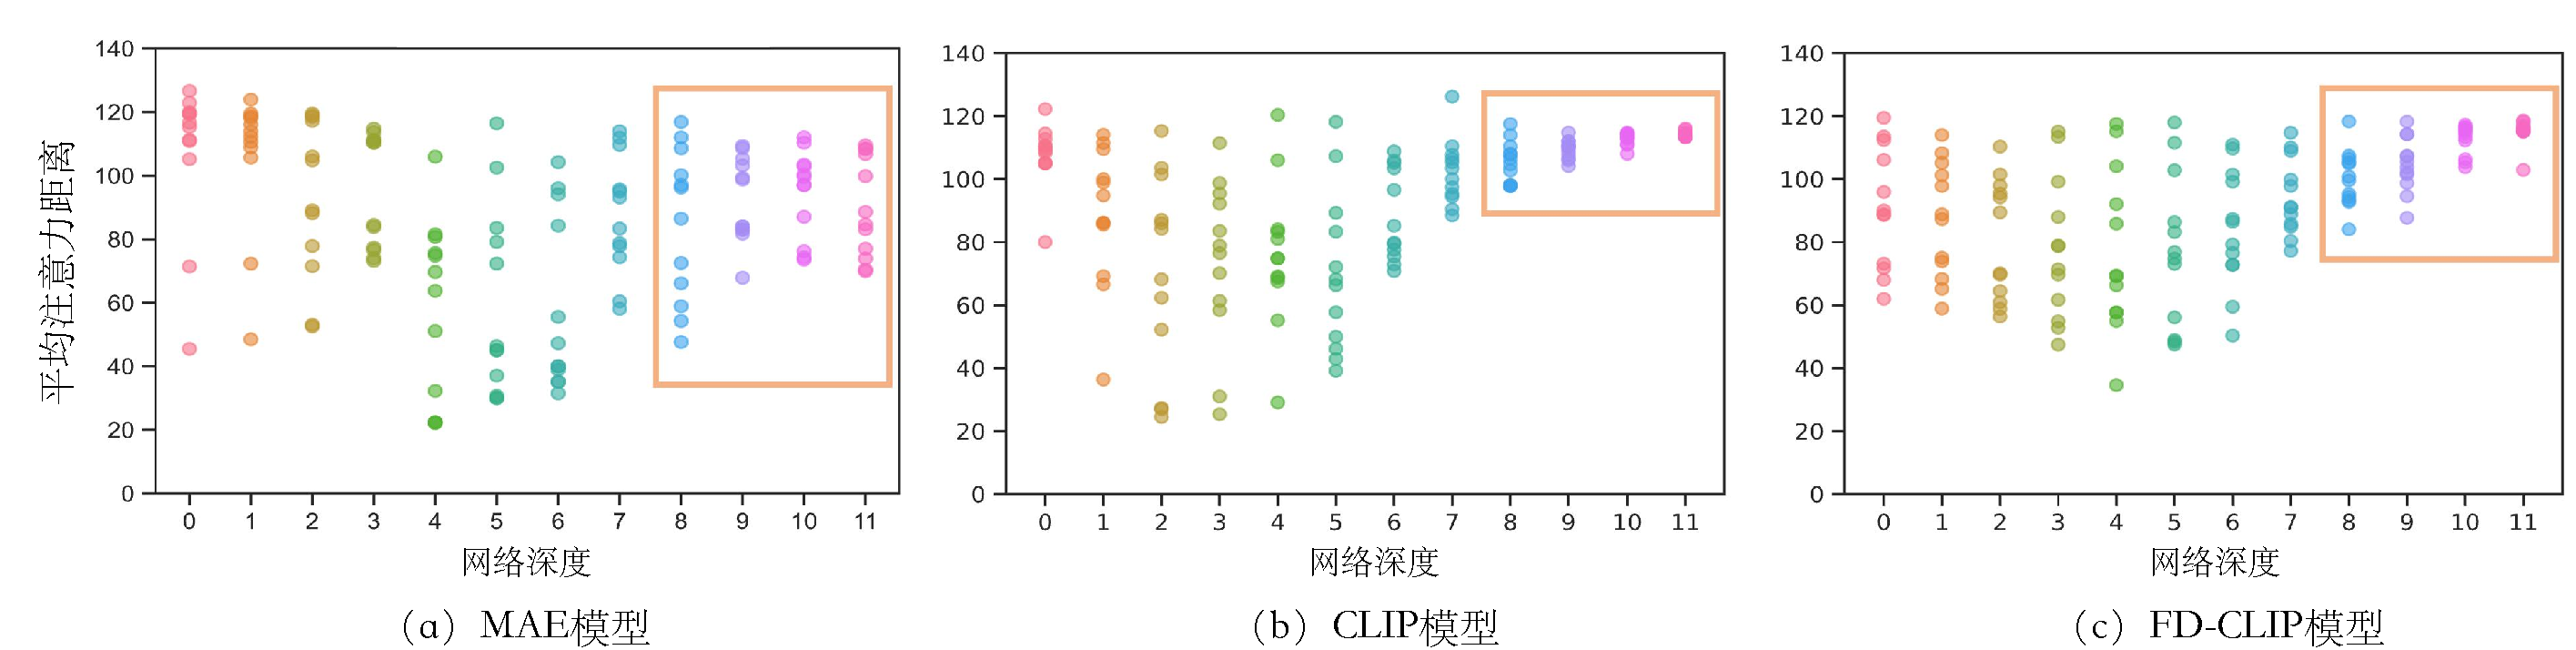
\includegraphics[width=1.0\linewidth]{figures/fd-attn-distance.pdf}
  \caption{不同预训练模型的平均注意力距离分布}
  \label{fig:fd-attn-distance}
\end{figure}
\paragraph{感受野多样化的注意力头} 该诊断工具分析了模型不同注意力头的图像感受野多样性。图\ref{fig:fd-attn-distance}分别展示了MAE模型、原始CLIP模型和经过特征图自蒸馏的FD-CLIP模型中不同网络深度的模型层内每个注意力头的平均注意力距离。
可以看到,在所有模型中,深度较浅的模型层里不同注意力头的感受野范围比较发散,说明此时模型既能建模局部的图像信息,又能获取全局的图像信息,展现了注意力头间的多样性。
然而,这种感受野的多样性在原始CLIP模型的较深模型层中迅速缩减。这表明模型的表达能力没有得到充分利用\cite{xie2023revealing}。
相比之下,FD-CLIP模型缓解了这个问题。FD-CLIP模型不同注意力头的感受野多样性在较深的模型层中保留得更好,也与MAE模型特征更为相似。%,表明它的模型容量可能被利用地更好。

\begin{figure}
  \centering
  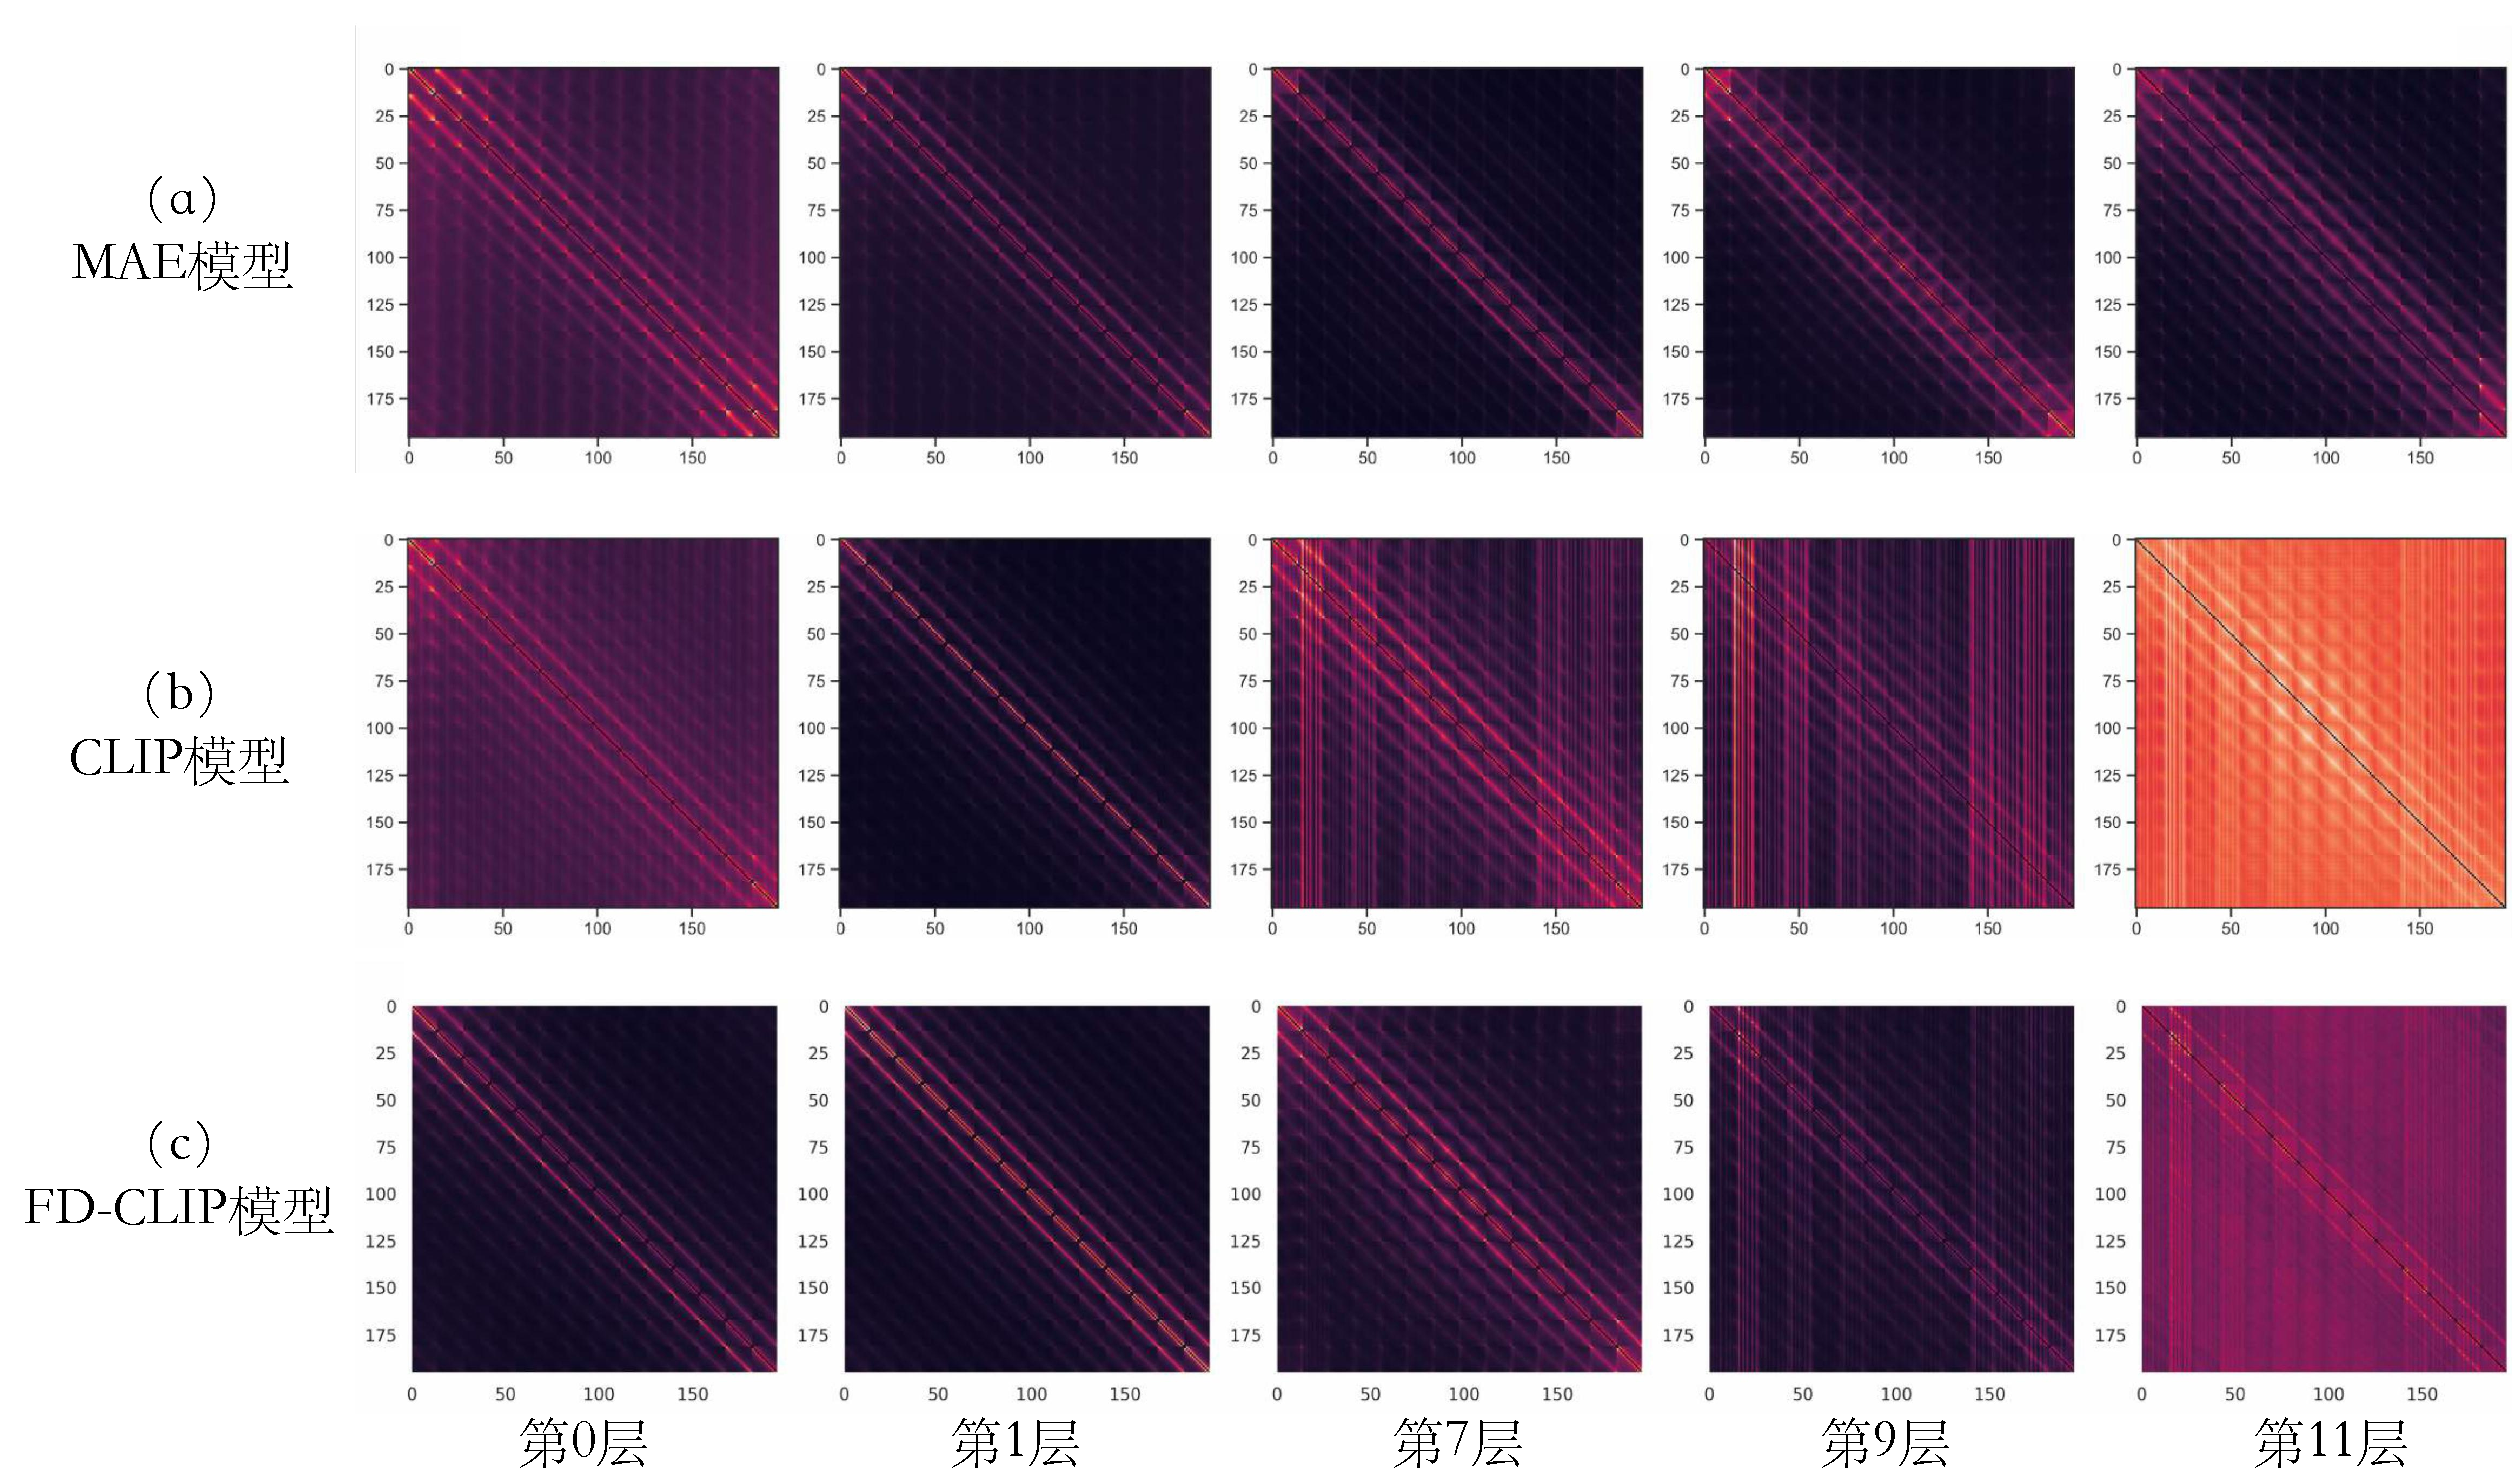
\includegraphics[width=1.0\linewidth]{figures/fd-attn-map.pdf}
  \caption{不同预训练模型的平均注意力图表现}
  \label{fig:fd-attn-map}
\end{figure}

\paragraph{平移不变性增强的注意力图} 图\ref{fig:fd-attn-map}展示了不同模型中某一层的平均注意力图。与原始CLIP模型相比,MAE模型的平均注意力图显示出更多的对角线模式,表明其更注重来自相对位置的视觉信息。这种特征属性表明掩码图像模型可以驱使模型学习到更强的视觉表征平移不变性。这种局部敏感性使得模型在需要密集感知能力的细粒度下游任务上有更好的迁移表现。
而CLIP模型在更深的层(7至11层)中展现出了更多垂直模式,这表明CLIP模型的视觉表征被一些处于绝对位置的输入像素主导。特征图自蒸馏之后,FD-CLIP模型的平均注意力图中垂直模式部分消失,视觉表征的平移不变性得到增强,与MAE模型特征更为相似,因此有助于提高其下游任务迁移性能。

\begin{figure}
  \centering
  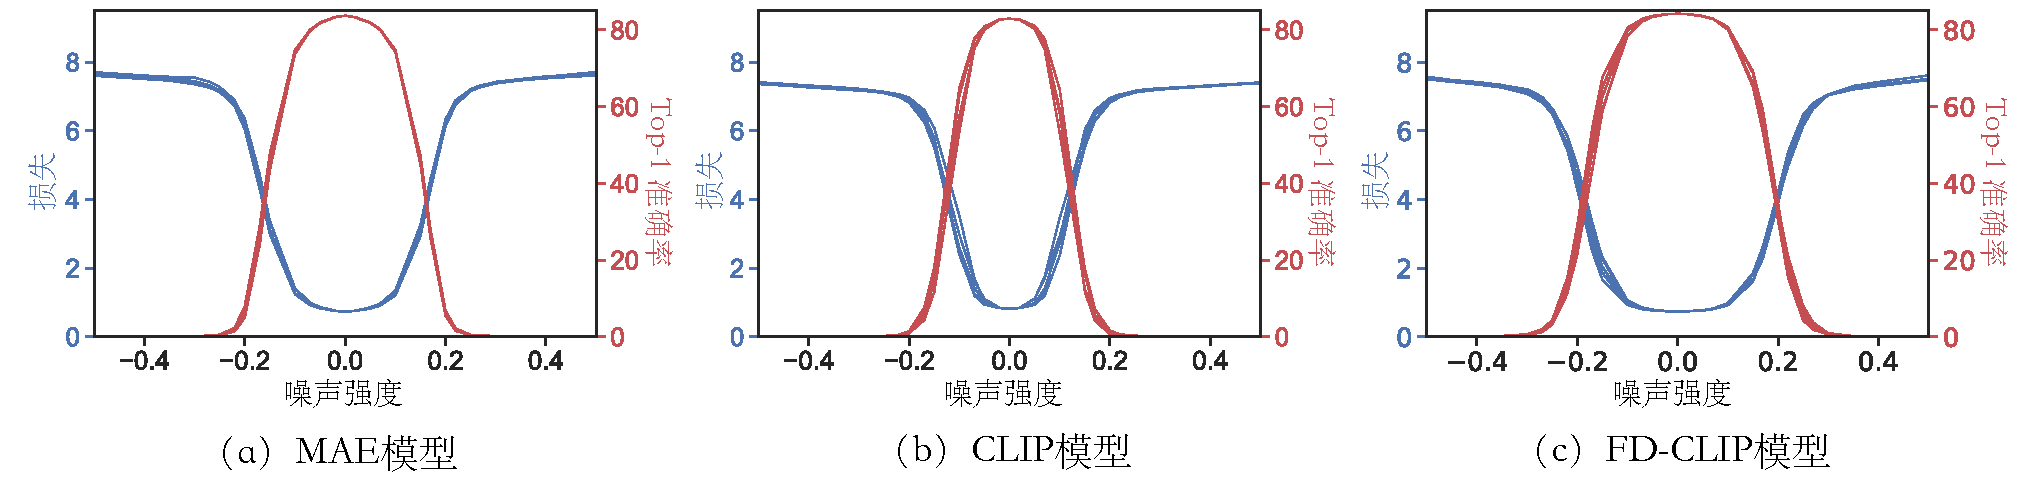
\includegraphics[width=1.0\linewidth]{figures/fd-loss-landscape.pdf}
  \caption{不同预训练模型的损失景观和准确率景观}
  \label{fig:fd-loss-landscape}
\end{figure}

\paragraph{损失景观的平坦化} 图\ref{fig:fd-loss-landscape}显示了不同模型在不同噪声强度影响下的损失景观和准确率景观\cite{li2018visualizing}。从可视化结果中可以看出,MAE模型和FD-CLIP模型的损失景观相比于原始CLIP模型的损失景观更加平坦,表明了经过特征图自蒸馏的模型在下游视觉任务的优化过程更加平稳,泛化性能更好。% 这一观察结果也与它在实验中更好的微调效果一致。

% 图 3:(a) MAE [17]、(b) CLIP [42] 和 (c) FD-CLIP 上每个头部在每一层深度的平均注意力距离。距离是在像素级别测量的。

% 图 4:(a) MAE [17]、(b) CLIP [42] 和 (c) FD-CLIP 上的平均注意力图。这些地图是所有头部和所有图像的平均值。选择五个代表性图层,即第 0、1、7、9、11 个图层,以节省空间。完整的注意力地图可以在补充材料中找到。

% 图5:(a)平均绝对误差(MAE)[17]、(b)对比语言-图像预训练(CLIP)[42] 以及(c)FD - CLIP的损失/准确率态势图[33],其中x轴表示噪声强度,y轴表示损失/准确率。每张图展示了使用5个随机生成方向得到的5个态势图。 

\begin{figure}
  \centering
  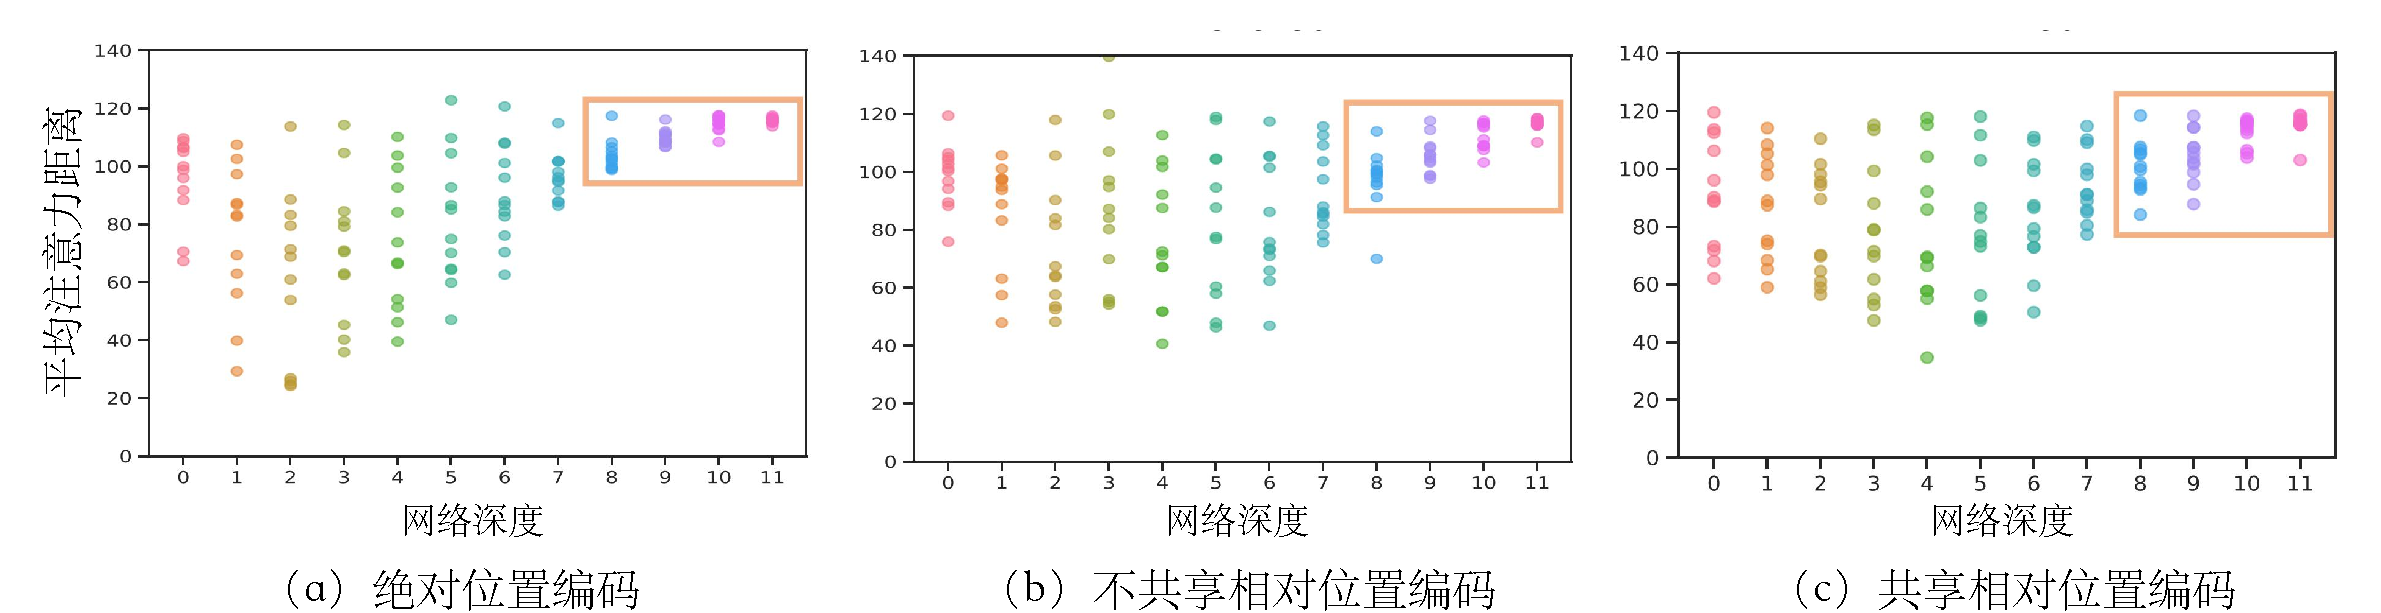
\includegraphics[width=1.0\linewidth]{figures/fd_compare_all_ape_rpe.pdf}
  \caption{不同位置编码策略的平均注意力距离分布}
  \label{fig:fd_compare_all_ape_rpe}
\end{figure}

\paragraph{位置编码策略对注意力头多样性的影响} 特征图自蒸馏方法在学生模型中引入了层间共享的相对位置编码设计,以减少在较深的模型层中出现不同像素表征间过于相似的现象。表\ref{tab:fd-ablation_tricks}(c)中的消融实验结果表明这种归纳偏置对CLIP模型的迁移性能有改进作用。
本节分析了在特征图自蒸馏过程使用不同位置编码配置的模型特征属性区别,包括绝对位置编码、不共享相对位置编码和共享相对位置编码。图\ref{fig:fd_compare_all_ape_rpe}中展示了在使用不同位置编码配置的情况下模型各注意力头的平均注意力距离分布。
与使用绝对位置编码和不共享相对位置编码的模型相比,使用共享相对位置编码的模型在更深的模型层中注意力头的感受野大小更加多样化,表明此时模型深层参数的冗余性更低。这一观察解释了这种共享相对位置编码具有更佳迁移效果的原因。


\section{总结}
\label{sec:fd-summary}


% CLIP 模型已经展示了令人印象深刻的高零镜头识别精度,但是,它们在下游视觉任务上的迁移性能并不理想。相反,尽管在训练过程中没有语义标签,但掩码图像模型 (MIM) 在对下游任务的微调方面表现异常出色。我们注意到这两个任务具有不同的成分:图像级目标与标记级目标,交叉熵损失与回归损失,以及全图像输入与部分图像输入。为了减少差异,我们引入了一个经典的特征图蒸馏框架,它可以同时保留 CLIP 模型的语义能力,同时构建一个包含 MIM 关键成分的任务。实验表明,特征图蒸馏方法显著提高了 CLIP 模型在几个典型的下游视觉任务上的迁移性能。我们还观察到该方法产生了新的 CLIP 表示,这些表示与 MIM 的表示具有一些共享的诊断特性。此外,特征图蒸馏方法推广到其他预训练模型,如 DINO、DeiT 和 SwinV2-G,在 MSCOCO 对象检测方面达到了 64.2 mAP 的新纪录,提高了 +1.1。

% 我们的贡献总结如下:
% ・我们研究了 CLIP 和 MIM 方法之间的成分差异,并证明靶标粒度对于 MIM 在微调中的成功至关重要。
% ・我们利用经典的特征图蒸馏将 CLIP 的训练目标粒度转换为令牌级的粒度,从而增强了其 performance 并保留其语义信息。
% ・我们在特征图自蒸馏过程中提出了几种进一步扩大改进的关键技术,包括蒸馏标准化特征图、不对称滴路径速率和共享相对位置偏置。
% ・通过多种诊断工具,我们发现与 CLIP 相比,MIM 和 FD-CLIP 都具有几个直观上良好的特性,这可能为它们卓越的迁移性能提供见解。
% ・我们将我们的方法推广到各种预训练模型,并观察到一致的收益。我们还通过使用我们的框架改进先进的 3B SwinV2-G 模型,创造了 MSCOCO 对象检测的新记录。

% 背景+motivation
语言-图像对比学习方法利用大规模图文数据对学习了丰富的语义信息,在零样本开放集合图像识别任务上表现优异。然而,CLIP方法在许多下游视觉任务,尤其是依赖密集感知能力的细粒度视觉任务上的迁移表现不佳。
% 前一章中提出的iCLIP方法通过引入已有的低噪声有标注数据,有效地扩展了CLIP模型训练可利用数据源的同时,显著提高了数据利用的效率。但这种方法得到的CLIP模型在迁移到下游视觉任务,尤其是细粒度视觉任务上的性能提升有限。
% 语言-图像对比学习方法利用大规模图文数据对学习了丰富的语义信息,因此在固定视觉模型只微调分类器的线性探测分类任务上可以取得非常优异的表现。然而,相比于像素级自监督方法,语言-图像对比学习方法得到的视觉模型在许多下游视觉任务,尤其是依赖密集感知能力的细粒度视觉任务上的迁移性能并无优势。

% 解决方案和发现
本章提出了特征图自蒸馏方法,将掩码图像模型的像素训练目标引入CLIP方法中,在无需大规模人工标注图文数据对和重新预训练CLIP模型的情况下,即可显著提升CLIP方法的细粒度视觉任务迁移性能。
该方法以CLIP模型自身作为教师模型,提取其输出特征图作为随机初始化的学生模型的训练目标。特征图自蒸馏方法一方面无需数据标注即可构造像素级训练目标,另一方面以较低代价将教师模型的知识转移到学生模型中。经过特征图自蒸馏的CLIP模型在语义分割、目标检测、深度估计等细粒度下游视觉任务上取得明显性能提升。将该方法推广到参数量达三十亿的SwinV2-G模型后,经过特征图自蒸馏的SwinV2-G模型取得了当时MSCOCO数据集上目标检测任务的新纪录。此外,本章还提出多种模型特征属性诊断工具对自蒸馏前后的模型进行分析,揭示了自蒸馏后的CLIP模型与掩码图像模型具有的相似性质,从而解释了特征图自蒸馏方法的有效性原因。
% 实验观察到像素级图像自监督预训练模型,如掩码图像模型(MIM),在下游任务上的迁移表现优异。受该类方法启发,本章仔细研究了两种不同预训练任务的建模区别,并着重讨论了输入图像完整性和训练目标粒度对视觉任务迁移性能的影响。
% 为低代价地在CLIP模型中引入像素级训练目标,同时避免大规模的数据标注以利用互联网级数据,本章提出使用特征图自蒸馏的方法,在尽可能保留CLIP模型中蕴含的语义信息同时引入像素级的监督目标。这种方法无须重新训练CLIP模型,且相比于原本CLIP模型训练代价而言,只需要额外3\%的训练成本即可显著提升其在各类下游任务,尤其是细粒度视觉任务上的性能表现。
% 通过在特征图自蒸馏框架中设计不同训练目标粒度和不同输入图像比例的实验,结果表明提升下游任务迁移性能的关键在于应用像素级的训练目标粒度。
% 此外,本章还提出利用多种注意力头级、模型层级、模型级的诊断工具对自蒸馏前后的模型进行分析和理解,可视化观察显示经过特征图自蒸馏的FD-CLIP在直观上拥有一些和MIM模型类似的特性,这为它们优异的迁移性能提供了见解。
% 为进一步验证该框架的通用性和可扩展性,本章将该框架用于不同视觉模型结构、不同预训练任务和不同模型规模的视觉模型,并观察到一致的收益。通过特征图自蒸馏框架改进的有三十亿参数的SwinV2-G模型,创造了当时MSCOCO数据集上目标检测的新纪录。

% 引出下一章
虽然本章工作提升了CLIP方法在下游视觉任务上的迁移性能,但其在语义生成任务上的迁移方式仍待探索。下一章以图像描述生成任务为主要场景,研究了CLIP方法在语义生成任务上的迁移方式,并提出了基于离散扩散模型的迁移方法。
% !TeX root = ../main.tex
\chapter{基于离散扩散模型的语义生成任务迁移方法}
\label{chap:ddcap}
% 这里一个难点是,怎么强调这个事情和CLIP强绑定,
% 也即解释完为什么要套离散版本而不是连续版本之后,
% 需要证明这个事情要和CLIP有关
%%%%%%%
% 一个思路是从Dalle-2出发,Dalle-2可以把Text-Feature Render成Image-Feature for Image-Generation
% 所以我们believe CLIP的Image-Feature可以Read Out Text Annotation;就是强调READ OUT和LiT一样
% 刚好前一章提到的事情就是还不知道怎么把CLIP模型迁移到以图像注释为例的图像生成中去;
% 强调captioning是一种重要的task,所有text生成,比如qa,common sense reasoning本质都是基于caption的一种特殊任务,只需要一个alignment
% 这一章就是借鉴Dalle-2,不过dalle-2两阶段:feature diffusion+raw pixel diffusion
% 这一章直接一阶段出raw text;
% dalle-2是continuous diffusion,我们是discrete diffusion(we also tried continuous diffusion,but not so work)
% 也有一些工作在clip模型后面加ar,这篇文章证明了相比ar来做text generation有一些额外的好处。
% 一个是加速,一个是edit这种特殊任务
%%%%%%%
% 图像字幕任务通常是通过一种逐个解码文本标记的自回归方法来实现的。我们提出了一种基于扩散的字幕模型,称为 DDCap,以实现更大的解码灵活性。与图像生成不同,图像生成中的输出是连续的、冗余的,具有固定长度,而图像标题中的文本是分类的,并且长度不同。因此,天真地将离散扩散模型应用于文本解码效果不佳,如我们的实验所示。为了解决性能差距,我们提出了几种关键技术,包括最佳优先推理、集中注意力掩码、文本长度预测和无图像训练。在没有额外字幕预训练的 COCO 上,它的 CIDEr 分数为 117.8,比受控设置中具有相同结构的自回归基线高 +5.0。在字幕填充任务中,它还执行比自回归基线 (230.3 vs. 203.5) 高 +26.8 的 CIDEr 分数。借助 4M 视觉语言预训练图像和基本大小的模型,我们在 COCO 上达到了 125.1 的 CIDEr 分数,这与最好的成熟自回归框架相比具有竞争力。该代码可在 https://github.com/buxiangzhiren/ DDCap 获取。

%%%%%%%%%%%%%%%%%%%
% 再介绍dalle-2的做法、介绍我们想read-out text,引出扩散模型
% 再介绍dalle-2里的图像扩散模型
% 扩散模型的好处,并行,修改
% 再介绍文本扩散模型的研究,介绍区别,困难和挑战
% 再介绍图像注释任务,图像描述在文本生成任务里的通用性等等(cite llava那些用captioning做pt的)
% 再介绍我们的工作

%%%%%%%%%% 前一章描述
% 虽然本章工作仔细研究了CLIP方法在下游视觉任务,尤其是细粒度视觉任务的迁移表现和改进方法,但如何将CLIP方法迁移到生成式多模态下游任务还不清楚。下一章将以图像注释这一通用任务为主要研究对象,研究CLIP模型实现生成式多模态任务的方法。
%%%%%%%%%%
语言-图像对比学习方法利用互联网图文数据对和实例级对比学习思想驱动模型训练,将视觉表征和语言表征映射到联合空间。CLIP方法得到的视觉表征具有强判别性,被广泛用于零样本开放集合图像识别和图文跨模态检索任务,经过迁移后也可用于目标检测、语义分割、深度估计等下游视觉任务。第\ref{cha:fd}章讨论了如何提升CLIP方法在下游视觉任务上的迁移表现,但未解决语义生成任务的迁移问题。因此,设计合适的迁移方法赋予CLIP方法语义生成能力是本章的研究目标。

\section{引言}
\label{sec:ddcap-intro}
CLIP方法通过对大规模视觉与语义信息进行建模和对齐,具备出色的物体、属性、位置等内容的感知能力,建立起视觉和语言表征间的桥梁,促进图像与文本模态的相互映射和转化。Dall-E 2方法\cite{dall-e2}正是利用了CLIP方法作为跨模态转化的桥梁来完成基于文本的图像生成任务。如图\ref{fig:ddcap-dalle2}所示,对于一段给定的文本,Dall-E 2方法的图像生成过程分为以下两步:
\begin{enumerate}
    \item 利用CLIP方法建立的模态对齐能力进行跨模态表征转化。Dall-E 2方法先利用CLIP方法的语言模型提取给定文本的语言表征,再训练一个基于扩散模型\cite{ddim,ddpm}的先验模型来预测对应的视觉表征。
    \item 将转化好的视觉表征重新映射回像素空间得到原始图像。由于CLIP视觉表征保留了丰富的图像信息,Dall-E 2方法利用一个基于扩散模型的图像解码器将这种视觉表征转化为原始图像。
\end{enumerate}

\begin{figure}
  \centering
  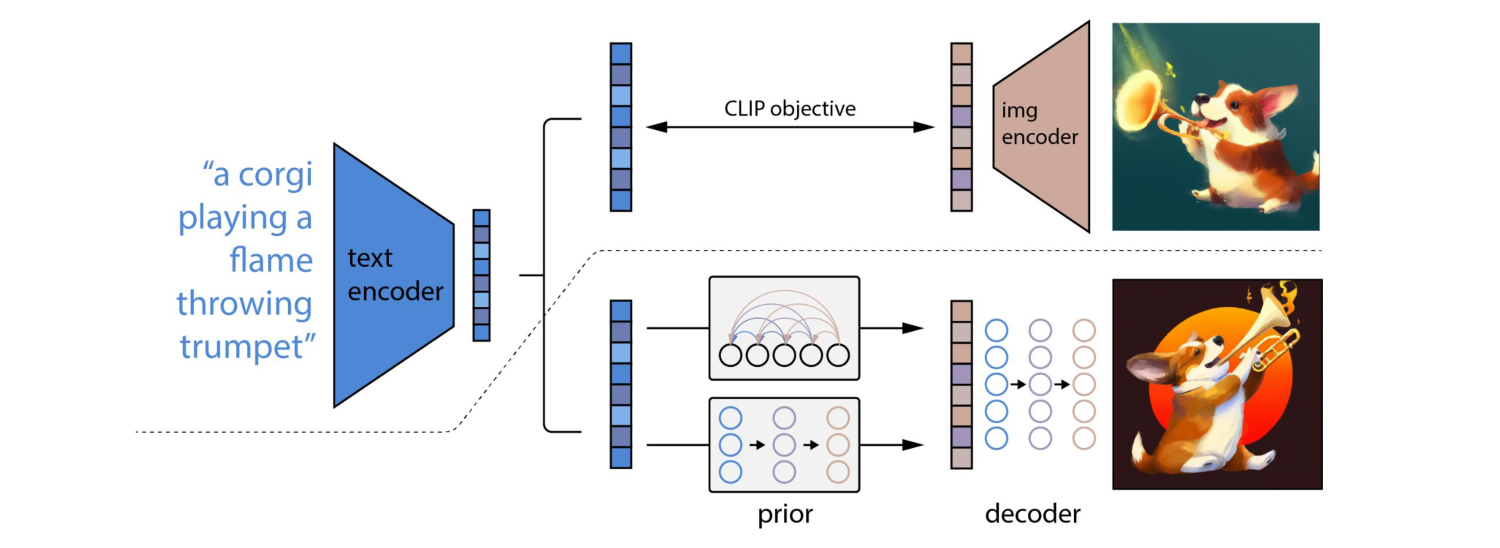
\includegraphics[width=1.0\linewidth]{figures/ddcap-dalle2-v2.pdf}
  % \caption{Dall-E 2方法将CLIP模型的文字表征转化为视觉表征后生成图像}
  \caption{Dall-E 2\cite{dall-e2}方法流程图}
  % 需要辅佐一张图像特征到文本生成的推广
  \label{fig:ddcap-dalle2}
\end{figure}

Dall-E 2方法将CLIP方法成功用于从语言表征到视觉表征的转化,证明CLIP方法得到的多模态表征间有很强的对应关系。这促使本章关注另一个问题:CLIP方法能否将视觉表征转化为语言表征,进而实现基于图像的语义生成任务迁移?值得注意的是,Dall-E 2在上述两个关键转化步骤中均采用了强大的扩散模型作为生成器。扩散模型\cite{ddpm, ddim}已成功用于各类无条件、基于图像类别或基于文本的图像生成任务\cite{beatsgan, glide, latentdiff, imagen},进而产生保真度高、多样性强的图像内容。相比于GAN\cite{gan}等传统生成方法,扩散模型引入迭代生成的思想,可以建模更复杂的数据分布,无需对抗训练而更稳定。相比于自回归的方法,扩散模型可以并行化生成以提高生成效率,并允许模型对已生成结果进行修改,避免了自回归方法因固定生成顺序而导致的误差累积问题。因此扩散模型已经逐渐成为图像生成任务的主流方法,并在现实场景中得到了大规模应用\cite{latentdiff, dall-e2}。

\begin{figure}
  \centering
  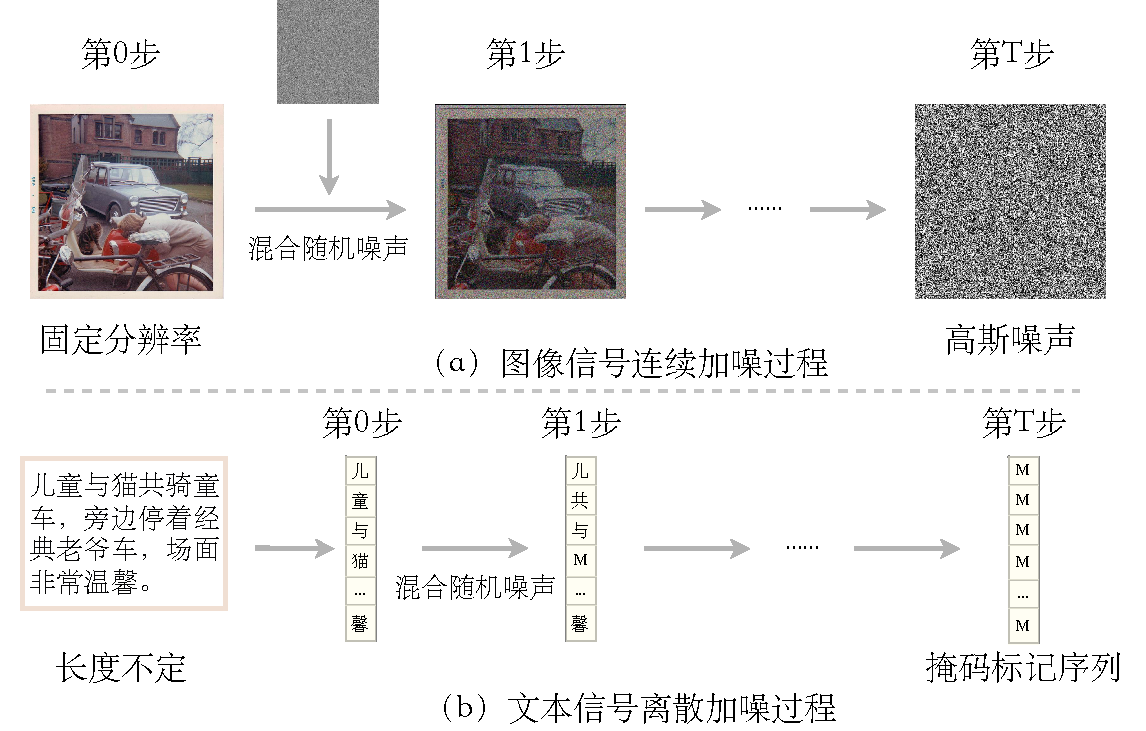
\includegraphics[width=1.0\linewidth]{figures/ddcap-img-text-diff.pdf}
  \caption{图像生成任务和文本生成任务在加噪过程中的区别}
    % 图 2.(a) 图像生成:噪声是连续的、冗余的,具有固定的长度 (b) 文本生成:噪声是分类的,而且很短,长度各不相同。
  \label{fig:ddcap-img-text-diff}
\end{figure}


然而,目前已有的研究中尚无直接有效的方法将扩散模型应用于基于图像的文本生成任务\cite{karpathy2015deep, vinyals2015show}。如图\ref{fig:ddcap-img-text-diff}所示,站在生成任务的视角,图像信号与文本信号存在几项固有的区别:
\begin{itemize}
    \item 信号在连续性和冗余性方面的区别。在图像生成任务中,因为输出图像除主体部分外往往包含信息密度更低的背景内容,因此,图像信号通常表现为具有连续且高度冗余特性。但在文本生成任务中,输出文本是离散且信息精炼的,通常不包含与图像内容无关的冗余信息。
    \item 信号序列长度可变性的区别。图像生成任务具有固定的输出分辨率,通常为$32^2$、$64^2$等固定尺寸。而且图像信号的连续特性使得调整图像分辨率相对容易实现\cite{dall-e2,super-resolution}。而文本生成任务则恰好相反,不同图像对应的文本信息长度多样。常见任务的文本长度在10到50之间不等。但文本信号的离散性使得对其长度进行类似图像分辨率调整的操作非常困难。
    \item 噪声建模方式的区别:扩散模型的推理过程是一个在输入中反复添加噪声并进行去噪预测的循环过程。由于图像信号的连续性和冗余性,在图像信号中添加噪声后,各个像素仍保有部分原始信息。因此模型可相对容易地利用信噪比较高的邻近像素信息进行预测。但在离散的文本信号中添加噪声后,正确文字可能会被直接替换为错误文字,此时单个文字的原始信息几乎完全丢失。因此对于文本生成任务而言,扩散模型的推理过程也需要特殊设计。
\end{itemize}

% 由文本扩散模型的困难介绍文本扩散模型的好处,以及引出我们为什么选择了图像注释任务
% 虽然利用扩散模型将CLIP的图像特征转化为文本特征仍有一定挑战,但由于扩散模型提供了并行生成的可能性,允许对上下文信息同时建模,并天然支持对中间结果进行修改,在行为自由度上和人类更为相似,这些优势促使本章对此进一步探索。
因此,本章系统地研究了基于扩散模型将CLIP方法迁移至下游语义生成任务的方法。前期实验表明,连续扩散模型在文本生成任务上表现欠佳,与主流自回归方法\cite{OSCAR,VinVL,UFO,ViTCap,SimVLM,GIT}相比性能差距明显。基于上述对文本信号离散特性的分析,本章主要讨论了离散扩散模型\cite{VQ-diffusion},并提出了更适合文本生成任务训练和推理过程的DDCap方法。在训练方面,DDCap方法引入长度预测任务,先预测待生成文本长度再进行推理,从而灵活适应不同长度的文本信号。考虑到文本的离散性和信息密集特性,DDCap方法在模型自注意力层中添加集中注意力掩码模块,使模型自适应地关注信息量更大的文本位置。在推理方面,DDCap方法设计了最佳优先推理策略,在每个扩散去噪步骤中保持已恢复的置信度最高的$K_{t}$个文本标记不变,避免它们在后续重新加噪过程中被改变。其中$K_{t}$值设置为待预测文本长度与推理步数的比值,使得模型在每一步中输出的信息量基本均匀。最后,受图像生成模型中无分类器引导方法\cite{glide}启发,DDCap方法引入无图像引导文本生成训练策略从而增强模型鲁棒性。具体而言,DDCap方法在训练过程中随机丢弃部分样本的图像输入以促使模型学习文本先验知识。在推理时,DDCap方法对基于文本先验知识的输出和以图像内容为条件的输出进行加权组合,获得与图像内容更相关的生成结果。
% 首先在训练方面,DDCap方法提出引入一个长度预测任务,实现先预测待生成文本长度,再进行推理过程的做法,从而更灵活地适应不同长度的文本信号。考虑到文本信号的离散特性和信息密集特性,DDCap方法提出在模型自注意力层中添加集中注意力掩码模块,以便模型自适应地专注于信息量更大的文本位置。其次在推理方面,DDCap方法中设计了一种称为最佳优先的推理策略。该推理方法保持每个扩散去噪步骤中恢复的最佳$K_{t}$个标记不变,使其不会在后续的重新加噪步骤中被替换为其他文本内容。
% % 换句话说,在每个扩散去噪步骤中定期选择一组标记固定下来不再改变,并在加噪步骤中,只对未标记为固定的标记集合添加噪声。
% 其中每个去噪步骤中保持的标记数目$K_{t}$大致设置为长度预测任务输出的文本长度与推理过程步数的比值。最后,受图像生成模型的无分类器引导方法\cite{glide}启发,DDCap方法提出引入无图像训练的文本生成方法以增强模型的鲁棒性。具体而言,DDCap方法在训练过程中会随机选择一些训练样本,将其图像输入丢弃后预测对应文本内容,以强制模型学习文本的先验知识。在推理过程中,DDCap方法可以对基于文本先验的输出和基于图像内容的输出进行加权组合,从而获得与图像内容联系更紧密的文本生成结果。

% 本章选取了最具有代表性的图像注释任务(Image Captioning)\cite{karpathy2015deep, vinyals2015show}作为主要研究对象。
% 图像注释任务是一种特殊的基于图像的文本生成任务,可作为辅助阅读手段,具有较强的现实意义。
% 同时,图像注释任务被认为是各类下游多模态任务的通用代理任务\cite{llava},如图文问答、物体定位等,因此提高图像注释能力对其他任务也有帮助。
% 此外,图像注释任务能够成为自动生成互联网替代文本的一种方式,进而反过来拓宽CLIP预训练数据的来源,从而形成数据飞轮\cite{blip-2}。

本章在图像描述生成任务\cite{karpathy2015deep, vinyals2015show}中验证DDCap方法,表明离散扩散模型能够有效地将CLIP视觉表征转化为语义输出,从而实现语义生成任务的迁移。在不失一般性的前提下,本章使用最常用的OpenAI CLIP\cite{radford2021learning}模型作为待迁移模型。在包含1000万图文对的数据集上对CLIP模型进行迁移训练后,DDCap方法在MSCOCO数据集\cite{chen2015microsoft}上取得了125.1的CIDEr-D分数\cite{cider},与多个先进自回归方法\cite{OSCAR,VinVL,UFO,ViTCap}结果相当,远优于基于连续扩散模型的迁移方法。
此外,这种基于离散扩散模型的语义生成任务迁移方法使得模型能够在生成图像描述过程中同时考虑上下文语境,并具备对已生成内容进行修改的能力。因此,本章还提出了更适合人机交互场景的描述修改任务,即删除已生成图像描述中的所有形容词,要求模型根据上下文重新预测被删除的内容,并使用CLIPScore\cite{CLIPScore}方法评估修改前后的图像描述与图像间的语义匹配程度。实验证明基于离散扩散模型的迁移方法相比自回归方法更能把握细微语义变化,在图像描述修改任务中表现更佳。

% 本章将DDCap方法在图像描述生成任务\cite{karpathy2015deep, vinyals2015show}中进行了验证,证明了利用离散扩散模型将CLIP模型的视觉表征转化为语义输出,并实现语义生成任务迁移的可行性。
% DDCap方法使用含有1000万个图像-描述对的数据集对CLIP模型进行微调后,在MSCOCO数据集\cite{chen2015microsoft}的图像描述生成任务上取得125.1的CIDEr-D\cite{cider}分数。这一结果与一些最先进的自回归模型\cite{OSCAR,VinVL,UFO,ViTCap}结果相当。
% 此外,这种基于离散扩散模型的语义生成任务迁移方法可以使得模型在生成图像描述时同时考虑上文和下文,并赋予了模型对已生成内容进行修改的能力。
% 因此,本章还提出了一项更适合人机交互场景的描述修改任务。在此任务中删除了已生成图像描述中的所有形容词,要求模型根据上下文去重新预测被删除的内容,并使用CLIP分数\cite{CLIPScore}来评估修改前后内容间的语义匹配程度。实验证明基于离散扩散模型微调的模型相比于基于自回归方法微调的模型更能把握细微的语义变化,并在描述修改任务中表现更佳。

综上所述,本章的主要内容安排如下:
\begin{itemize}
    \item 第\ref{sec:ddcap-intro}节讨论了图像生成领域中的扩散模型,以及文本信号区别于图像信号的关键特性:离散性、低冗余性、序列长度可变性。
    \item 第\ref{sec:ddcap-method-all}节介绍了用于语义生成迁移的离散扩散模型基本思想,以及针对文本信号特性设计的训练与推理方法:集中注意力掩码模块、长度预测任务和最佳优先推理策略,以及无图像引导文本生成训练策略。
    \item 第\ref{sec:ddcap-result}节介绍了本章的实验设置、评测指标和实验结果,并介绍了图像描述修改任务设置与测试结果。
    \item 第\ref{sec:ddcap-summary}节对本章内容进行了总结。
\end{itemize}

% 因此,本文的贡献总结为
% • 我们是第一个将离散扩散模型应用于图像描述的公司,并提供了第一个证据,证明扩散模型可以达到与最好的、完善的自回归模型相比的竞争性能。
% • 我们提出了四个关键设计:(i) 长度预测用于处理文本生成中的可变长度问题;(ii) 集中注意力掩码用于提取紧凑的文本信息,而不会受到不需要的噪音的干扰;(iii) 提出了最佳优先推理以减少污染正确生成的令牌的机会;(iiii) 无图像训练,以平衡文本先验和图像条件中的信息。
% • 我们进一步展示了离散扩散模型在标题填充任务中的优势。

% 本文的其余部分组织如下。我们在第 2 节中总结了相关工作。第 3 节提出了拟议的 DDCap 模型的细节。第 4 节报告了大量的实验结果,包括定量和定性讨论。我们最后在第 5 节中得出结论。


\section{研究方法}
\label{sec:ddcap-method-all}
本节介绍了基于离散扩散模型的语义生成任务迁移方法DDCap。第\ref{sec:ddcap-method}节首先讨论了将离散扩散模型应用于图像描述生成任务的基本思想。第\ref{sec:ddcap-key-design}节详细阐述了针对文本信号的离散性、低冗余性和序列长度可变性设计的关键训练和推理方法。

% 本节详细介绍了基于离散扩散模型实现CLIP模型在语义生成任务上微调的DDCap方法。
% 与当前主流的自回归方法相比,这种方法具有更大的解码灵活性。例如,这种方法允许同时预测多个标记,而不是逐个预测,前文标记也可以依赖后文标记进行生成并修改,而不是仅只允许按阅读顺序进行生成。
% 第\ref{sec:ddcap-method}节首先介绍了将离散扩散模型应用于图像描述生成任务的基本思想。第\ref{sec:ddcap-key-design}节接着详细介绍了多种针对文本信号的离散性、冗余特性、序列长度可变性设计的训练和推理方法,对提高性能起到了关键作用。

\subsection{基于离散扩散模型实现语义生成任务的基本思想}
\label{sec:ddcap-method}
连续扩散模型在每个图像像素上单独施加连续高斯噪声,因此可以精确且连续控制各元素的噪声强度。与连续扩散模型不同,离散扩散模型则在实例级别控制整体噪声强度,通过对单个元素进行掩码或替换操作实施加噪过程。对标记化后的文本序列而言,离散扩散模型通过将文本标记替换为掩码标记[\texttt{MASK}]或其他随机文本标记来实现加噪。当文本标记被替换为随机标记时,该输入元素的信噪比显著降低,而当该文本标记被进一步被替换为掩码标记时,输入元素的原始信息几乎完全丢失,仅作占位符用途。因此,受文本信号离散性特点影响,离散扩散模型无法连续调节单个输入元素的噪声强度,而是通过控制掩码标记比例来调节整个输入序列的噪声水平。

% 连续扩散模型将连续高斯噪声单独施加在每个图像像素之上,因此输入模型的每个元素都可以连续控制不同的噪声强度。与连续扩散模型不同,离散扩散模型通常在实例级别实行加噪过程,以控制其整体噪声强度。对单个元素而言,离散噪声通常以掩码或替换的形式实现。对标记化后的文本序列而言,离散扩散模型使用掩码标记[\texttt{MASK}]或其他随机正常文本标记替换当前的文本标记作为加噪方法。
% 一旦当前的文本标记被替换为其他随机的正常文本标记,该输入元素的信噪比就降到了很低的水平。如果该文本标记被进一步替换为掩码标记,则此时该输入元素的原始信息几乎完全丢失,只起到了占位符的作用。
% 因此,离散扩散模型无法连续控制单个输入元素的噪声强度,而是通过控制掩码标记比例来控制输入序列的整体噪声水平。
% \todo{目前的符号里混杂了标记x和标记序列x,也混合了gt的x和预测的$\hat{x}$}

\paragraph{加噪过程} 本章使用GPT-2模型的分词器\cite{gpt2}将图像描述文本转化为文本标记序列。图像描述中的每个文本标记记作$x$,是一个有5万多种可能取值的离散变量。

离散扩散模型的加噪过程可以描述为一个一阶马尔可夫过程。每个离散的马尔可夫状态跳转都在逐步增加文本标记序列的噪声水平。将对文本标记$x$加噪$t$步后得到的标记表示为$x_{t}$,初始状态$x_0=x$。在每一加噪步中,正常文本标记都有一定概率转换为掩码标记,而掩码标记作为特殊的吸收状态,一旦转变为此状态将不再改变。因此,如果$x_{t-1}$不是掩码标记,那么在第$t$个加噪步中$x_{t-1}$到$x_t$的状态转移概率定义为:
% 离散扩散模型的加噪过程可以被认为是一个仅依赖前一步状态的马尔可夫过程,逐步地增加文本标记序列的噪声水平。将对文本标记$x$加噪了$t$步得到的标记表示为$x_{t}$,可以得到$x_0=x$。
% 在每一个加噪步中,任何正常文本标记都有一定概率被转换成掩码标记。而掩码标记是一种特殊的吸收状态。任何已经转变为掩码标记的$x_{t}$将一直停留在掩码标记状态。因此,如果$x_{t-1}$还不是掩码标记,那么在第$t$个加噪步中$x_{t-1}$的状态转移概率定义为:
\begin{equation}
    q(x_t | x_{t - 1}\neq\texttt{[MASK]}) = 
    \begin{cases}
    \alpha_t, & x_t = x_{t - 1} \\
    \gamma_t, & x_t = \texttt{[MASK]} \\
    1 - \alpha_t - \gamma_t, & \text{其他情况}.
    \end{cases}
    \label{eq:iclip-q-nonmask}
\end{equation}

具体而言,在第$t$个加噪步中,$x_{t-1}$有$\alpha_{t}$的概率保持原文本标记不变,有$\gamma_{t}$的概率转换为掩码标记,还有$\beta_{t}=1-\alpha_{t}-\gamma_{t}$的概率随机转换为词汇表中其他文本标记,这些不同文本标记的转移概率相同。若$x_{t-1}$已经是掩码标记[\texttt{MASK}],在第$t$个加噪步中$x_{t-1}$到$x_t$的状态转移概率定义为:
% 具体而言,在第$t$个加噪步中,$x_{t-1}$有$\alpha_{t}$的概率保持原文本标记不变,有$\gamma_{t}$的概率被转换成掩码标记,同时还有$\beta_{t}=1-\alpha_{t}-\gamma_{t}$的概率被随机转换成词汇表中的其他文本标记。
% 如果$x_{t-1}$已经是掩码标记[\texttt{MASK}],由于其是一个吸收状态,在第$t$个加噪步中$x_{t-1}$的状态转移概率定义为:
\begin{align}
    q(x_t | x_{t - 1} = \texttt{[MASK]}) = 
    \begin{cases}
    1,& x_t =\texttt{[MASK]} \\
    0,& \text{其他情况}.
    \end{cases}
    \label{eq:iclip-q-mask}
\end{align}

当反复对文本序列施加公式\eqref{eq:iclip-q-nonmask}和\eqref{eq:iclip-q-mask}中的加噪过程,且总步数$T$足够大时,所有文本标记最终都会转变为掩码标记。这种状态也是推理过程的开始状态。
% 通过对整个文本序列反复施加公式\eqref{eq:iclip-q-nonmask}和公式\eqref{eq:iclip-q-mask}中描述的加噪过程,只需要总步数$T$足够大,最终所有文本标记都会转变为掩码标记。% 这也是推理阶段的起点。

% \begin{figure}
%   \centering
%   
\includegraphics[width=1.0\linewidth]{figures/placeholder.pdf}
%   \caption{DDCap模型结构示意图}
%   % image encoder; decoder (cross-attn) + time step
%   \label{fig:ddcap-arch}
% \end{figure}

\paragraph{去噪过程} 
去噪过程是加噪过程的逆过程。离散扩散模型的去噪过程从全掩码标记序列开始,逐步施加去噪步以恢复原始输入信号,最终得到完整的图像描述。因此,离散扩散模型训练的主要目标即是对该去噪过程建模,表示为:
\begin{equation}
\max_{\theta} p_{\theta}(x_{t-1} | x_{t}, y),
  \label{eq:ddcap-target}
\end{equation}
其中$y$为从CLIP视觉表征,$\theta$为待训练的模型参数。

本章采用Transformer\cite{Transformer}模型结构作为模型$\theta$,以建模文本序列的去噪过程。为了以视觉表征$y$为条件输出$x_{t-1}$,本章考虑两种方式:
\begin{itemize}
    \item 在输入序列维度上拼接视觉表征$y$与待去噪文本序列$x_{t}$,并用Transformer模型结构的自注意力机制进行建模;
    \item 用交叉注意力机制,将视觉表征$y$的信息逐层融合进待去噪文本序列$x_{t}$中;
\end{itemize}
本章实验采用第二种建模方式,既避免了视觉表征与文本序列位置编码融合的问题,又增强了待去噪文本序列对视觉表征的关注度。
% 整体结构示意图如图\ref{fig:ddcap-arch}所示。

为在不同去噪步$t$时激发不同的模型行为$\theta_t$,本章遵循图像生成扩散模型\cite{VQ-diffusion}的一般做法。该做法将去噪步$t$信息编码为正余弦位置嵌入后,注入模型的自适应层归一化模块\cite{adaln}中,进而改变该模块对特征的缩放和偏移参数,达到激发不同模型行为的目的。模型不同维度$i$的正余弦位置嵌入方式如下:
\begin{equation}
    \text{PE}_{i} = \begin{cases}
    \sin(\frac{p}{10000^{2i/d_{\text{model}}}}), i < \frac{d_{\text{model}}}{2} \\
    \cos(\frac{p}{10000^{2i/d_{\text{model}}}}), i \ge \frac{d_{\text{model}}}{2},
    \end{cases}
    % emb = self.linear(self.silu(self.emb(timestep))).unsqueeze(1)
    % scale, shift = torch.chunk(emb, 2, dim=2)
    % x = self.layernorm(x) * (1 + scale) + shift
    \label{eq:ddcap-t}
\end{equation}
其中$p = t/T\times \text{step}_{\text{scale}}$,而$d_{\text{model}}$是模型隐藏层维度。$\text{step}_{\text{scale}}$作为调整正余弦函数周期的超参数,其值越大,模型在不同去噪步间的行为差异越显著;反之,模型行为则更为一致。
% 其中$d_{\text{model}}$是模型隐藏层维度,$p = t/T\times \text{step}_{\text{scale}}$。
% $\text{step}_{\text{scale}}$是一个调整正余弦函数周期的超参数。越大的$\text{step}_{\text{scale}}$值会放大模型在不同去噪步$t$之间的行为差异,越小的值则会使得模型在不同去噪步$t$间的行为更一致。
%在本章实验中一般设$\text{step}_{\text{scale}}$为8000。

\paragraph{训练过程} 训练过程的核心是使模型$\theta_t$对第$t$步的去噪过程进行建模。连续扩散模型通常采用预测噪声形式为学习目标,而离散扩散模型由于在句子级别控制噪声强度并通过掩码或替换策略实施加噪过程,无法直接将单元素噪声转化为可学习目标。受已有工作\cite{structddm}启发,DDCap方法以直接预测原始文本标记$x_{0}$为学习目标,损失函数为:
% 训练过程本质是驱动模型$\theta_t$对去噪过程进行建模。在连续扩散模型中,去噪过程的学习目标通常是预测噪声形式,而离散扩散模型通过掩码或替换策略在句子级别控制不同的噪声强度,因此无法将单元素的噪声转化成可学习目标。
% 受已有工作\cite{structddm}启发,DDCap方法的实际训练目标为直接预测原始文本标记$x_{0}$。损失函数形式如下:
\begin{equation}
\mathcal{L}=-\log p_{\theta_t}(x_0 | x_t, y).
\end{equation}

% 而公式\eqref{eq:ddcap-target}中描述的去噪过程建模目标,可以通过如下重参数化技巧\cite{VQ-diffusion}得到:
公式\eqref{eq:ddcap-target}中的去噪过程建模目标可通过重参数化技巧\cite{VQ-diffusion}转化得到:
\begin{equation}
    p_{\theta_t}(x_{t-1} | x_{t}, y)=\sum_{\hat{x}_0=1}^{V}q(x_{t-1}|x_{t},\hat{x}_0)p_{\theta_t}(\hat{x}_0 | x_{t}, y),
\end{equation}
其中$V$表示所有可能的文本标记总数,$\hat{x}_0$表示模型基于当前第$t$步输入对原始文本标记$x_{0}$的预测结果。而$q(x_{t-1}|x_{t},\hat{x}_0)$可通过贝叶斯公式求得:
\begin{equation}
    q(x_{t-1}|x_{t},\hat{x}_0)=\frac{q(x_{t}|x_{t-1},\hat{x}_0)q(x_{t-1}|\hat{x}_0)}{q(x_{t}|\hat{x}_0)}=\frac{q(x_{t}|x_{t-1})q(x_{t-1}|\hat{x}_0)}{q(x_{t}|\hat{x}_0)}.
\end{equation}

DDCap方法的训练过程如图\ref{fig:ddcap-train-inference}的左侧部分所示。

\paragraph{推理过程} 离散扩散模型的推理过程从一个完全由掩码标记[\texttt{MASK}]组成的序列$x_{T}$开始,应用模型$\theta_{T}$习得的去噪过程得到预测结果$\hat{x}_{0}$,并对其重新加噪得到$x_{T-1}$。循环往复$T$步之后,即可得到最终预测结果。因此,与自回归方法在序列维度进行迭代不同,离散扩散模型在噪声强度维度进行迭代。

从$x_{t}$推理出$x_{t-1}$的单步去噪过程计算如下:首先,利用训练好的模型$\theta_t$根据CLIP视觉表征$y$和当前文本序列通过$p_{\theta_t}(x_{0} | x_{t}, y)$估计出$\hat{x}_{0}$;其次,利用加噪过程的马尔可夫性推导出$x_{t-1}$的分布并进行采样。具体公式为:
\begin{equation}
    q(x_{t-1} | \hat{x}_{0})=\prod \limits_{i=1}^{t-2} q(x_{i+1} | x_i)\cdot q(x_1 | \hat{x}_{0}).
\end{equation}

由于在离散扩散模型推理过程的每一中间步中,模型均给出了基于当前噪声输入的原始文本序列预测$\hat{x}_{0}$。因此,离散扩散模型支持通过快速采样方式加速推理过程,从而在$T$步内获得较准确的预测结果。DDCap方法的推理过程如图\ref{fig:ddcap-train-inference}的右侧部分所示。
% 离散扩散模型通过不断的加噪和去噪的循环,在$T$步之后得到最终预测结果$\hat{x}_{0}$。由于每一个中间步中,模型均给出了基于当前噪声输入下对原始文本序列的预测结果,因此离散扩散模型允许通过一些快速采样的方式对推理过程进行加速,使其在小于$T$步之内得到较为准确的预测结果。DDCap方法的推理过程如图\ref{fig:ddcap-train-inference}的右侧部分所示。

\begin{figure}
  \centering
  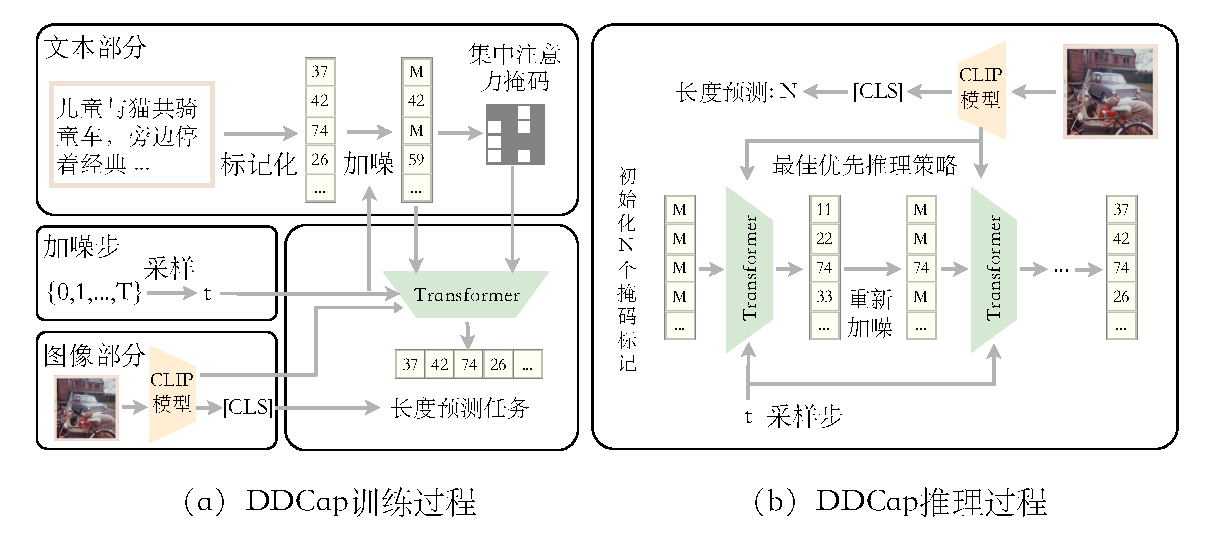
\includegraphics[width=1.0\linewidth]{figures/ddcap-train-inference.pdf}
  \caption{DDCap方法训练过程和推理过程示意图}
  % image encoder; decoder (cross-attn) + time step
  \label{fig:ddcap-train-inference}
\end{figure}

%%%%%%%%%%%%
\subsection{针对文本信号特性的关键设计}
\label{sec:ddcap-key-design}
前期实验表明,仅采用上述简单设计时,离散扩散模型在语义生成任务迁移性能上远弱于自回归方法,难以生成完整且有意义的图像描述。根据第\ref{sec:ddcap-intro}节对图像和文本信号特性的分析,这是因为文本生成与图像生成任务存在显著差异,所以将图像生成任务的离散扩散模型直接用于文本生成任务无法取得较好的迁移性能。
首先,待生成文本长度多变,而图像分辨率通常固定。其次,文本信息较为紧凑,单个文本标记的改动可能导致整段文本意义完全改变或表意不明,而图像中的冗余信息较多,相邻像素间的连续性可提供互证信息。此外,由于离散扩散模型中引入掩码标记[\texttt{MASK}]和标记替换策略实施加噪过程,因此文本标记间的语义离散性使得单个输入元素的噪声强度近似为阶跃函数:一旦该文本标记被替换或掩码,几乎无法保留任何原始信息。而在图像生成任务中,图像解码器提供一定的冗余性,使得单个标记承载的信息可通过其他标记所反映。基于这些观察,本节提出四种针对文本生成任务的关键设计:长度预测任务、集中注意力掩码模块、最佳优先推理策略和无图像引导文本生成训练策略。

% 前期实验发现,仅通过上述设计的简单实现,离散扩散模型相比于自回归模型方法在语义生成任务迁移上表现较弱,几乎无法生成完整有意义的图像描述。
% 根据第\ref{sec:ddcap-intro}节中的对图像信号和文本信号特性的分析,文本生成任务与图像生成任务有相当大的不同。
% 首先,待生成文本的长度多变,而待生成图像的分辨率通常是固定的。
% 同时,文本中的信息比较紧凑,单个文本标记改动之后可能会使得整段文本具有截然不同的意思或出现表意不明的现象,但是图像中的冗余信息较多,不同像素之间由于邻域内的连续性可以提供互相印证的信息。
% 此外,由于离散扩散模型中引入掩码标记[\texttt{MASK}]和标记替换来构造噪声,因此不同文本标记之间语义的离散性导致对单个文本标记而言,其噪声强度近似是一个阶跃函数:一旦被替换为别的文本标记或掩码标记,该文本标记上的信噪比接近于0。但是对于基于离散扩散模型的图像生成任务而言,后续的图像解码器提供了一定的冗余性,使得当前图像标记承载的信息可以通过别处的图像标记所反映。
% % 每个像素上的噪声强度可以被连续控制,不会出现完全不提供信息的情况。
% 受这些观察启发,本节提出了以下四种针对文本生成任务的关键设计:长度预测任务、集中注意力掩码模块、最佳优先推理策略和无图像引导文本生成训练策略。

\paragraph{长度预测任务} 自回归方法中,文本标记序列从左到右依次生成,直至出现表示结尾的终止标记[\texttt{EOS}]。而离散扩散模型作为并行生成方法,没有表示方向性的顺序概念。虽然可以仿照自回归生成方法,在离散扩散模型中直接引入终止标记,并仅将其左侧标记视为有效生成内容,但实验表明这种简单做法效果较差。这一结果表明离散扩散模型难以掌握正确的终止标记用法,容易出现提前终止的情况。
% \paragraph{长度预测任务} 在自回归方法中,文本标记序列从左到右依次生成,直到出现表示终止的特殊标记[\texttt{EOS}]为止。然而,离散扩散模型是一种并行生成方法,没有从左到右或从右到左的顺序概念。仿照自回归生成方法,可以直接在离散扩散模型中引入终止标记[\texttt{EOS}],并只将其左侧的文本标记视为有效标记。但实验发现这种简单做法的性能较差,因为模型很难掌握正确的终止标记用法,非常容易出现提前终止的情况。

本节提出将长度预测作为训练任务的一部分来解决此问题。因此,DDCap方法引入一个轻量化模型分支。该分支基于CLIP视觉表征预测待生成图像描述的序列长度,从而摆脱对终止标记的依赖。具体而言,长度预测任务利用CLIP方法的视觉模型中用于聚合图像全局信息的特殊标记[\texttt{CLS}]的对应表征作为输入,经多层感知机变换后输出预测序列长度。DDCap方法将长度预测任务建模为分类任务,并使用交叉熵损失函数训练。因为这个新引入的模型分支参数量小,所以长度预测任务不会造成过多额外的训练开销,而且因为该任务的训练梯度不会回传到CLIP方法的视觉模型,所以该任务不会影响其视觉表征提取能力。推理时,模型使用预测长度来初始化掩码序列,无需使用最大可能序列长度作为输入,从而在一定程度上加速了推理过程。

% 本节提出将长度预测本身作为训练任务的一部分来解决这个问题。DDCap方法引入了一个额外的轻量化模型分支来基于视觉表征预测待生成图像描述的序列长度,从而摆脱对终止标记[\texttt{EOS}]的依赖。
% 具体来说,在CLIP方法的视觉模型中有一个用于聚合图像全局信息的特殊标记[\texttt{CLS}],长度预测任务以[\texttt{CLS}]标记对应的视觉表征为输入,经过一个简单的多层感知机对表征进行变换后,输出预测的序列长度。DDCap方法将长度预测任务建模为一个分类任务,并使用交叉熵函数进行训练。% \todo{需要确认这里怎么做的交叉熵}
% 由于这个长度预测任务的参数量很小,因此不会引入很多额外的训练代价。同时这项任务的训练梯度不会进一步回传到CLIP方法的视觉模型的主体部分,使其不会干扰视觉模型提取视觉表征的能力。
% 在推理过程中,模型使用长度预测任务输出的序列长度来初始化全掩码标记序列,避免使用最大可能的标记序列长度作为初始化,因此在一定程度上加速了推理过程。

\begin{figure}
  \centering
  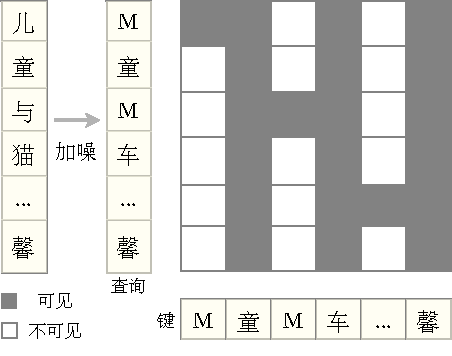
\includegraphics[width=0.6\linewidth]{figures/ddcap-attn.pdf}
  \caption{DDCap方法集中注意力掩码模块示意图}
  % image encoder; decoder (cross-attn) + time step
  \label{fig:ddcap-attn}
\end{figure}

\paragraph{集中注意力掩码模块} 前文分析指出,文本信号的离散特性导致在加噪过程中被转换为掩码标记[\texttt{MASK}]的文本标记除了作为占位符外无法提供有用信息。这一问题在训练过程加噪步数$t$较大时或推理阶段初期尤为严重。因为此时输入文本序列噪声强度大,大部分标记由掩码标记组成,所以对其他文本标记的学习造成了干扰。
% 前文分析到由于文本信号具有离散特性,若在加噪过程中某一文本标记被转换为掩码标记[\texttt{MASK}],那么该文本标记除了作为一个占位符以外无法对其他文本标记的预测提供任何有用信息。
% 这一问题在训练过程加噪步数$t$较大时,或者在推理过程的开始阶段尤为严重,因为此时输入的文本序列大部分内容由这种掩码标记组成,反而对其他正常文本标记造成干扰。

为解决此问题,DDCap方法提出集中注意力掩码模块方法。该方法通过修改注意力掩码控制模型的注意力分布,使所有位置的标记主要关注信息丰富的位置。如图\ref{fig:ddcap-attn}所示,在集中注意力掩码模块设计中,正常文本标记在自注意力机制中仅与其他正常文本标记交换信息,不与信息匮乏的掩码标记交互;而掩码标记之间也不互相影响,只从自身和正常文本标记中收集预测所需信息。这种集中注意力掩码模块提高了有噪声文本序列中有效信息间的交互效率,避免了无效信息干扰。实验表明,这种新颖的注意力掩码设计显著提升了图像描述生成任务性能。

% 为了解决这个问题,DDCap方法提出集中注意力掩码模块设计,通过修改注意力掩码来对模型注意力位置进行控制,使得所有位置的文本标记主要关注有信息量的位置。
% 如图\ref{fig:ddcap-attn}所示,对于正常文本标记而言,它在模型自注意力机制中只与其他正常文本标记进行信息交换,而不与信息含量极低的掩码标记进行交互,而对于掩码标记而言,它们之间也不会互相影响,而是主要从有信息量的正常文本标记中收集可用于自身预测的信息。% \todo{这里可以配一个图}, 对ablation里的说明也有好处。
% 通过这种集中注意力掩码的方式,DDCap方法增强了有噪声文本序列中有效信息交互的效率,避免了无效信息的干扰。实验表明这种新颖的注意力掩码设计对图像描述生成任务的性能有较大帮助。

\paragraph{最佳优先推理策略} 推理过程中,离散扩散模型每步都会针对当前输入$x_t$应用去噪过程,给出对原始文本标记$x_0$的预测结果,并通过进一步加噪和去噪的迭代过程改进对原始文本标记的预测。为鼓励模型在推理过程中尽可能保留有用信息,DDCap方法提出最佳优先推理策略。该策略在每个去噪步$t$中均会保留一定比例模型置信度高的文本标记预测结果,防止其被重新加噪,为后续生成提供更多有效信息。
具体而言,设$N_{L}$为长度预测任务给出的待生成文本序列长度。若$N_{L}\le T$,则推理过程总步数从加噪步$T$减至序列长度$N_{L}$,从而在推理过程中的每步保留置信度最高的一个文本标记。若$N_{L}>T$,则在去噪步$t$时保留$K^{t}$个置信度最高的文本标记不被重新加噪。$K^{t}$的计算方法为:
\begin{equation}
    K^{t} = \lfloor \frac{T-t+1}{T}\times N_{L}\rfloor-\lfloor \frac{T-t}{T}\times N_{L}\rfloor.
\end{equation}

% \paragraph{最佳优先推理策略} 在推理过程中,去噪网络每一步都会给出对原始文本标记序列$x_0$的预测结果,并逐渐通过进一步加噪和去噪来改进这一预测,使其更加准确。为了鼓励模型在每步推理中尽可能保留有用的信息,DDCap方法提出了一种最佳优先推理策略,使得模型在推理过程的每一个去噪步中均保留一定比例置信度较高的文本标记不被重新加噪,而这些文本标记可以为下一步生成提供有用信息。
% 具体而言,设$N_{L}$为长度预测任务给出的待生成文本标记序列长度。如果$N_{L}\le T$,则推理过程总步数会从$T$步减少到$N_{L}$步,这样在推理过程中每一个去噪步都会保留预测出来的文本序列中置信度最高的一个文本标记。
% 同时,自适应层范数中使用的阶跃索引 t 也按比例缩小。% 对于t的处理细节可以先不提
% 如果长度预测任务给出的预测长度$N_{L}$大于训练时的总加噪步数$T$,那么最佳优先推理策略会在每一个去噪步$t$中保持$K^{t}$个置信度最高的文本标记不被重新加噪。$K^{t}$的计算方法如下:
% \begin{equation}
%     K^{t} = \lfloor \frac{T-t+1}{T}\times N_{L}\rfloor-\lfloor \frac{T-t}{T}\times N_{L}\rfloor.
% \end{equation}
\paragraph{无图像引导文本生成训练策略} 图像描述生成质量受模型两个关键能力的影响,一方面是模型将视觉表征转化为文本的能力,另一方面是模型对语言信号的建模能力。受图像生成方法中的无分类器引导方法\cite{glide, VQ-diffusion}启发,DDCap方法引入无图像引导文本生成训练策略。该策略通过在训练过程中将部分图像描述任务转化为纯文本生成任务,增强了扩散模型对语言信号本身的建模能力。
具体而言,在训练过程中,无图像引导文本生成训练策略以概率$r$将CLIP视觉表征替换为可训练的随机特征$e$,指示模型学习纯文本生成任务。此时损失函数修改为:
\begin{align}
    \mathcal{L}' = -\log p_{\theta_t}({x}_{0} | {x}_{t}, {e}).
\end{align}

% \paragraph{无图像引导文本生成训练策略} 图像描述生成任务受模型两个关键能力的影响,一方面是模型将视觉表征转化为文本表征的能力,另一方面则是模型对语言建模的能力。为了增强扩散模型对语言信号本身的建模能力,受无分类器引导的图像生成方法\cite{glide, VQ-diffusion}启发,DDCap方法在图像描述生成任务中使用了类似的无图像引导文本生成训练策略,在训练过程中将一定比例的训练任务转化为不基于图像条件的纯文本生成任务。具体来说,在训练过程中,CLIP方法的视觉模型输出的视觉表征以一定的概率$r$被替换为一个可训练的随机特征$e$,来指示模型此时需要学习一个纯文本生成任务:$p_{\theta_t}(x_{0} | x_{t}, e)$。此时,模型的损失函数对应修改为:
% \begin{align}
%     \mathcal{L}' = -\log p_{\theta_t}({x}_{0} | {x}_{t}, {e}).
% \end{align}
通过无图像引导文本生成训练策略,模型能更专注于学习文本生成任务本身,增强了其语言建模能力。在推理过程中,模型可在有图像条件与无图像条件的文本描述输出间进行插值,从而控制生成的图像描述对图像的依赖程度。外推该插值函数可以增强图像描述生成过程对图像内容的关注程度,从而达到增强生成效果的目的,概率分布计算如下:
% 通过引入无图像引导的训练方法,模型可以更专注于学习如何生成文本内容,并增强其对语言建模的能力。在推理过程中,模型可以在有图像条件的文本生成和无图像条件的文本生成两种不同情况的输出间进行插值,以控制图像描述生成过程对图像的依赖程度。如果将插值过程外推,可以取得增强图像描述生成能力的效果,对应的概率分布计算如下:
\begin{equation}
    \log p_{\theta_t}({x}_{0} | {x}_{t}, {y})'=\log p_{\theta_t}({x}_{0} | {x}_{t}, {e}) + \\ s(\log p_{\theta_t}({x}_{0} | {x}_{t}, {y}) - \log p_{\theta_t}({x}_{0} | {x}_{t}, {e})),
\end{equation}
其中$s$表示图像描述生成过程对图像信息的依赖程度,$s=0$时退化为纯文本生成任务,也即不依赖CLIP视觉表征的图像描述生成任务。通常$s$的取值范围为$[1, +\infty)$:$s=1$时等价于标准图像描述生成过程,而$s>1$时模型加强对视觉表征的关注,此时通常可以得到更佳的描述生成效果。在实验中,$s$的取值略大于1。
% 其中$s$表示图像描述生成过程中对图像信息的依赖程度,当$s=0$时回退为纯文本生成任务。通常而言$s$的取值范围为$[1, +\infty)$。当$s=1$时,插值结果等价于标准图像描述生成任务的输出结果,而当$s>1$时,模型将加强对视觉表征的关注程度,此时往往会取得更佳的描述生成效果。在实验中,$s$的取值略大于1。


\section{实验结果}
\label{sec:ddcap-result}
\subsection{实验设置}
\label{sec:ddcap-exp-setting}
% CLIP模型预训练过程将大规模的图像特征与文本特征进行对齐,因此CLIP预训练得到的文本模型以判别能力为主,不适合图像注释这类文本生成任务,同时原始文本模型中没有交叉注意力模块,无法基于图像特征进行生成。
本节实验从OpenAI CLIP模型\cite{radford2021learning}出发,随机初始化用于文本生成任务迁移的离散扩散模型参数,并在CLIP-Base和CLIP-Large两个不同大小的视觉模型上进行了实验验证。
为了充分训练随机初始化的离散扩散模型,使其能更好地把CLIP视觉表征转化为文本输出,本节引入两个阶段的图像描述任务训练。第一阶段使用一个较大规模的图文数据集对新初始化的离散扩散模型进行训练,第二阶段则在MSCOCO图文数据集上进行微调并测试。为节约计算开销,消融实验只包含了第二阶段。

\paragraph{第一阶段训练设置} 按照通常的做法\cite{uniter, meter},本节将MSCOCO\cite{chen2015microsoft}、Conceptual Captions\cite{sharma-etal-2018-conceptual}、SBU\cite{sbu}和Visual Genome\cite{krishna2017visual}四个数据集中的所有图文数据对合并,构建了一个包含大约400万张图像和1000万个相关文本的通用数据集作为这一阶段的训练数据。
此阶段训练的主要超参数设置如下:使用峰值学习率为1e-4的线性衰减学习率调度,设置批大小为1024并训练了15轮次。在此阶段中,CLIP方法的视觉模型以一个更小的学习率一起训练,从而进一步增强其视觉表征的表达能力。% 最长注释长度为$20$

\paragraph{第二阶段训练设置和评测方法} 
这一阶段中使用主流的MSCOCO图文数据集进行训练和测试。MSCOCO图文数据集共包含12万张图像,每张图像配有5条图像描述。遵循通常的训练集、验证集和测试集拆分方法\cite{karpathy2015deep},该阶段使用其中的11万图像和对应的描述集合进行训练,并利用另外5000张图像进行验证,最终在剩余的5000张图像上测试模型的图像描述生成效果。
由于语义生成任务不存在标准答案,本节实验使用常见文本生成评测指标进行测试,比对了模型输出与参考描述间的相似性。本节实验使用的指标为CIDEr-D\cite{cider}、BLEU@4\cite{bleu}、METEOR\cite{meteor}、ROUGE-L\cite{rouge}和SPICE\cite{spice},从单词匹配度、公共子序列长度、语义相似性等方面对模型输出的质量进行评测。在后续实验中,这些指标被分别简称为“C”、“B@4”、“M”、“R”和“S”。
% 不同指标说明:https://juejin.cn/post/7412894237019389991

此阶段训练的主要超参数设置如下:使用峰值学习率为2e-4的线性衰减学习率调度,设置批大小为512并训练30轮次。若模型经过第一阶段的训练,则在此阶段中对模型使用1e-5的峰值学习率进行微调。% 最长注释长度为$20$

\subsection{针对关键设计的消融实验}
本节的所有消融实验使用第二阶段进行训练并在MSCOCO数据集的验证集中进行测试。为了降低计算成本,此阶段CLIP方法的视觉模型不会进行更新。%,以单独评价不同设计方法在语义生成任务上的迁移性能优劣。

\begin{table}
  \centering
  \caption{DDCap方法针对文本信号特性关键设计的消融实验}
  \begin{tabular}{lccccccccc}
    \toprule   
    序号  & 推理 & 掩码 & 长度 & 无图像引导 & C & B@4 & M & R & S \\    
    \midrule
    \#1  &&&&& 20.6 & 7.4  & 18.8 & 34.6 &12.3  \\ 
    \#2  &&$\checkmark$&&& 43.6 & 11.4  & 20.5 & 39.1 & 14.4  \\ 
    \#3   &$\checkmark$ &&&& 45.2 & 20.3  & 26.9 & 47.3 & 21.3  \\
    \#4 &$\checkmark$&&$\checkmark$& & 92.6 & 27.3  & 25.4 & 51.8 & 18.7\\
    \#5  &$\checkmark$&$\checkmark$&&& 97.5 & 28.2  & 28.1 & 54.0 & \textbf{21.7} \\
    \#6  &$\checkmark$&$\checkmark$&$\checkmark$&& 116.7 & 34.6  & 28.1 & 57.4 & 21.5\\
    \#7 &$\checkmark$&$\checkmark$&$\checkmark$&$\checkmark$& \textbf{117.8} & \textbf{35.0}  & \textbf{28.2} & \textbf{57.4} & \textbf{21.7}\\
    \bottomrule
  \end{tabular}
  \label{tab:ddcap-component}
\end{table}

\paragraph{关键设计的消融} 
\label{sec:ddcap-exp-abl}
如第\ref{sec:ddcap-key-design}节所述,DDCap方法引入以下四种设计来增强离散扩散模型在图像描述生成任务上的效果:长度预测任务(简称为“长度”)、集中注意力掩码模块(简称为“掩码”)、最佳优先推理策略(简称为“推理”)和无图像引导文本生成训练策略(简称为“无图像引导”)。

表\ref{tab:ddcap-component}展示了四种关键设计形成各类组合的消融实验,其中序号\#1实验作为基准,不使用任何针对文本信号特性的设计。实验结果表明不引入任何针对性设计的离散扩散模型无法有效实现CLIP方法的语义生成任务迁移。对比序号\#3和\#1的实验结果,可以看出应用最佳优先推理策略将CIDEr-D分数从20.6提高到45.2,说明在推理过程中保留有用信息,使其不被重新加噪的重要性。

通过对比序号\#5和\#3的实验结果,可以看出集中注意力掩码模块对文本生成离散扩散模型的重要性。引入集中注意力掩码模块后,CIDEr-D分数从45.2进一步跃升到97.5。这一现象说明集中注意力掩码模块通过对低信息量的掩码标记进行特殊处理,对模型建模去噪过程产生了明显的积极影响。% 这一点正是由文本信号的离散性和信息紧致性特点导致的。

通过对比序号\#6和\#5的实验结果,可以看出长度预测任务对图像描述生成效果的影响。引入长度预测任务有助于模型做好提前规划,并增强其判断何时终止生成文本序列的能力。相比于序号\#5的实验,该设计将模型的CIDEr-D分数提高了近20点,表明此时模型生成的图像描述在语义上与参考描述更接近。但这种方法不影响模型对语法词序等内容的建模能力,因此METEOR指标没有变化。

最后,对比序号\#7和\#6的实验结果说明无图像引导文本生成训练策略对模型性能也有一定的提升。考虑到这种方式不会带来额外的训练开销,因此DDCap方法中默认使用了此项设计。
% \todo{既然前面说了什么各种字符匹配、语义匹配的评测维度,这里也可以加下不同策略的提升方面}


\begin{table}
  \centering
  \caption{DDCap方法对集中注意力掩码模块的消融实验}
  \begin{tabular}{lccccccc}
    \toprule
    方法  & M2M & T2M & C & B@4 & M & R & S\\
    \midrule
    DDCap &$\checkmark$&$\checkmark$& 92.6 & 27.3  & 25.4 & 51.8 & 18.7  \\ 
    DDCap &$\checkmark$&& 94.1 & 27.2  & 25.7 & 52.1 & 18.9  \\ 
    DDCap  & &$\checkmark$& 115.6 & 34.2  & 27.9 & 57.2 & 21.4  \\
    DDCap  && & \textbf{116.7} & \textbf{34.6}  & \textbf{28.1} & \textbf{57.4} & \textbf{21.5}\\
     \midrule
    DDCap($t < T/2$) &&& 98.8 & 29.8  & 25.2 & 52.8 & 19.4\\
    DDCap($t\geq T/2$)  &&& 112.9 & 33.2  & 27.9 & 56.5 & 21.2\\
    \bottomrule
  \end{tabular}
  \label{tab:ddcap-maskatten}
\end{table}

\paragraph{进一步理解集中注意力掩码模块的设计} 表\ref{tab:ddcap-component}中的消融实验展示了集中注意力掩码模块对图像描述生成任务性能的增强效果。在第\ref{sec:ddcap-method}节方法介绍中提到,这一模块设计的出发点是为了减少低信息量的掩码标记对其他正常文本标记的信息获取能力造成影响。该模块主要通过两部分设计修改了模型内部的信息交换机制:1)正常文本标记不从掩码标记中接收信息;2)掩码标记之间不交换信息。为了进一步理解文本生成离散扩散模型内的最优信息流动机制,表\ref{tab:ddcap-maskatten}中引入如下四种设置:
\begin{itemize}
    \item “M2M”意为允许掩码标记之间互相交换信息。
    \item “T2M”意为允许正常文本标记从掩码标记中获取信息。
    \item “$t < T/2$”意为对$t$较小的加噪步中应用集中注意力掩码模块。此时输入文本序列中掩码标记的比例较低。
    \item “$t\geq T/2$”意为对$t$较大的加噪步中应用集中注意力掩码模块。此时输入文本序列中的掩码标记比例较高。
\end{itemize}
 
表\ref{tab:ddcap-maskatten}展示了不同信息流动机制对模型性能的影响。实验发现,禁止掩码标记之间互相交换信息与禁止正常文本标记从掩码标记中获取信息两种方式都对模型性能有明显帮助,其中前者设计对模型性能有更显著的影响。造成这一现象的原因是,在离散扩散模型中掩码标记本身仅起到占位符的作用,而不同占位符之间除位置编码略有不同之外,内部表征非常相似。这种相似性可能会使得模型将不同位置的掩码标记混淆,从而导致错误的预测结果。此外,因为掩码标记本身信息含量很低,所以允许正常文本标记从掩码标记中获取信息并不会对该文本标记的预测有帮助。因此,文本生成离散扩散模型的最优信息流动方向应该是从高信息的正常文本标记流向其他正常文本标记或低信息的掩码标记。

与此同时,通过对比在低噪声训练步或高噪声训练步中引入集中注意力掩码模块的两组实验结果表明,在高噪声训练步中引入该方法对性能提升更加显著。因为此时输入文本序列中的掩码标记比例更高,所以模型更容易出现不同掩码标记间混淆的情况。这一结果也验证了对文本生成离散扩散模型内最优信息流动方向的猜测。

\begin{figure}
  \centering
  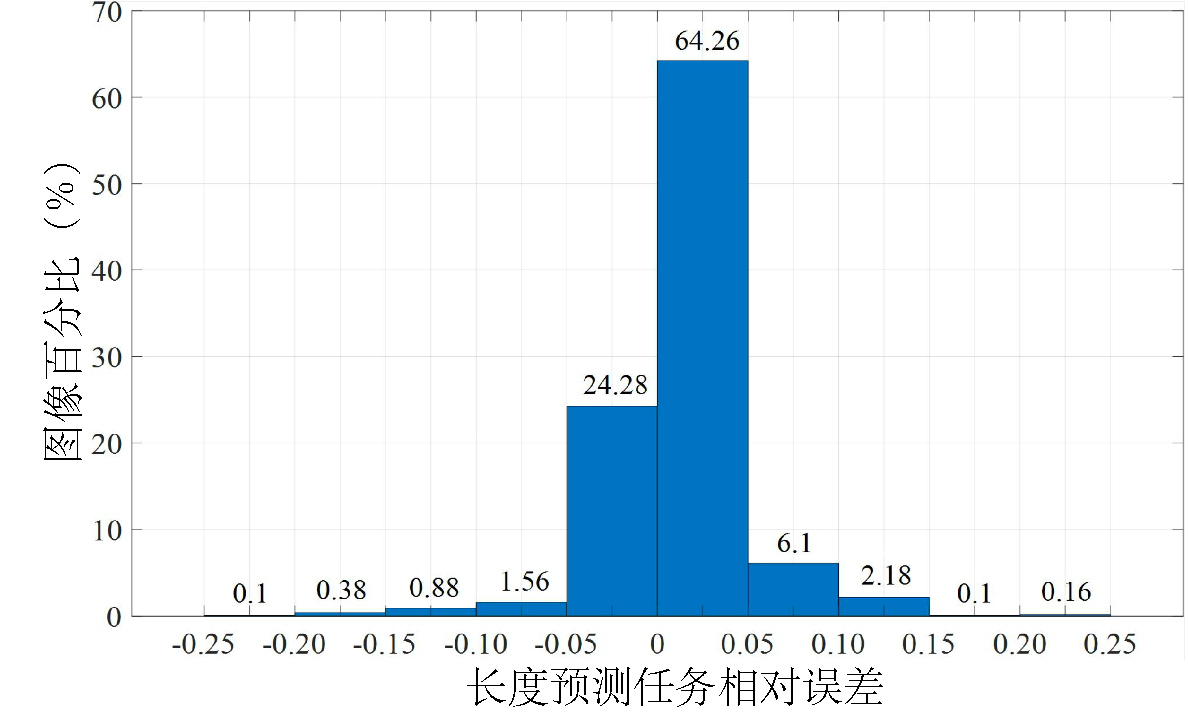
\includegraphics[width=0.7\linewidth]{figures/ddcap-length.pdf}
  \caption{DDCap方法长度预测任务的相对误差分布}
  % image encoder; decoder (cross-attn) + time step
  \label{fig:ddcap-length}
\end{figure}

\paragraph{长度预测任务的准确率} 图\ref{fig:ddcap-length}展示了DDCap方法在长度预测任务上的相对误差分布。相对误差的计算方式为$(N_{L}-N_{G})/N_{G}$,其中$N_{L}$表示模型预测的序列长度,$N_{G}$为实际序列长度。
% \todo{每个图像有5个注释文本,这玩意儿是咋测的} 是training统计吗?
统计结果表明有90\%的图像描述序列长度预测误差率在5\%以内。考虑到实验中最大序列长度为20,5\%的相对误差对应着误差一个文本标记,因此该长度预测任务的准确率在可接受范围内。

\begin{table}
  \centering
  \caption{DDCap方法中不同时间信息嵌入方式的对比实验}
  \begin{tabular}{lcccccc}
    \toprule
    方法 & $\text{step}_{\text{Scale}}$ & C & B@4 & M & R & S\\
    \midrule
    无信息嵌入 & - & 115.5 & 34.2  & 28.0 & 57.3 & 21.3\\
    自适应层归一化嵌入 & - & 115.1  & 34.1 & 28.0 & 57.1 & 21.3\\
    正余弦位置嵌入 & 4000 & 115.9 & 34.5  & 28.0 & \textbf{57.4} & 21.4\\
    正余弦位置嵌入 & 6000 & 114.8  & 33.7  & 27.9 & 57.0 & \textbf{21.5}\\
   正余弦位置嵌入 & 8000 & \textbf{116.7}  & \textbf{34.6}  & \textbf{28.1} & \textbf{57.4} & \textbf{21.5}\\
   正余弦位置嵌入 & 10000 & 115.1  & 34.0  & 27.9 & 56.9 & 21.3\\
    \bottomrule
  \end{tabular}
  \label{tab:ddcap-adaptivet}
\end{table}

\paragraph{去噪步时间信息嵌入方式的对比实验} 
在第\ref{sec:ddcap-method-all}节方法介绍中提到扩散模型在不同的去噪步$t$下会表现出不同的模型行为,以实现对不同噪声强度的自适应处理。如公式\eqref{eq:ddcap-t}所示,DDcap方法使用正余弦位置嵌入方法将去噪步信息传入到模型中。
表\ref{tab:ddcap-adaptivet}展示了正余弦位置嵌入方法与不引入去噪步时间信息的基线以及自适应层归一化嵌入方法的比较结果。结果表明,适当调整正余弦位置嵌入方法的$\text{step}_{\text{scale}}$值可以在一定程度上提升CLIP方法在图像描述生成任务上的迁移性能。将$\text{step}_{\text{scale}}$设为0时,实验结果与不引入去噪步时间信息的基线等价。实验表明适当区分不同去噪步间的模型行为对图像描述生成任务性能有一定帮助。

% \paragraph{无图像训练} 超参数(即r 和 s)的影响如图 4 所示。当训练比率 r 为 0.2 且推理量表为 1.17 时,我们的模型取得了最佳性能。值得注意的是,最佳指导比例范围与通常设置为 5 的图像生成范围不同 [64]
\begin{table}
  \centering
  \caption{CLIP方法与其他预训练方法在语义生成任务上的迁移性能比较}
  \begin{tabular}{lccccc}
    \toprule
    视觉预训练方法  & C & B@4 & M & R & S\\
    \midrule
    DINO & 99.3  & 29.6 & 25.9 & 53.6 & 19.3 \\
    DeiT & 100.7 & 29.6 & 25.9 & 53.9 & 19.5 \\
    CLIP  & \textbf{117.8} & \textbf{35.0} & \textbf{28.2} & \textbf{57.4} & \textbf{21.7}\\
    \bottomrule
  \end{tabular}
  \label{tab:ddcap-cmp-clip}
\end{table}

\paragraph{CLIP方法与其他预训练方法在语义生成任务上的迁移性能比较}
表\ref{tab:ddcap-cmp-clip}中展示了CLIP方法的视觉模型与其他主流视觉模型在语义生成任务上的迁移性能对比。实验结果表明,CLIP方法在图像描述生成任务上的表现明显优于DINO\cite{dino}和DeiT\cite{deit}等自监督或图像分类预训练方法。在CIDEr-D指标上,CLIP方法达到了117.8的得分,比DINO和DeiT分别高出18.5和17.1;在BLEU@4指标上,CLIP方法也获得了35.0的较高分数,明显优于其他两种方法。这一结果充分证明了CLIP方法通过语言-图像对比学习获取的视觉表征,对语义生成任务具有显著优势。这是因为CLIP方法在预训练阶段已经学习了图像与文本之间的语义对应关系,所以模型能够更准确地将视觉表征映射到相应的文本描述,为语义生成任务奠定了良好基础。

\begin{figure}
  \centering
  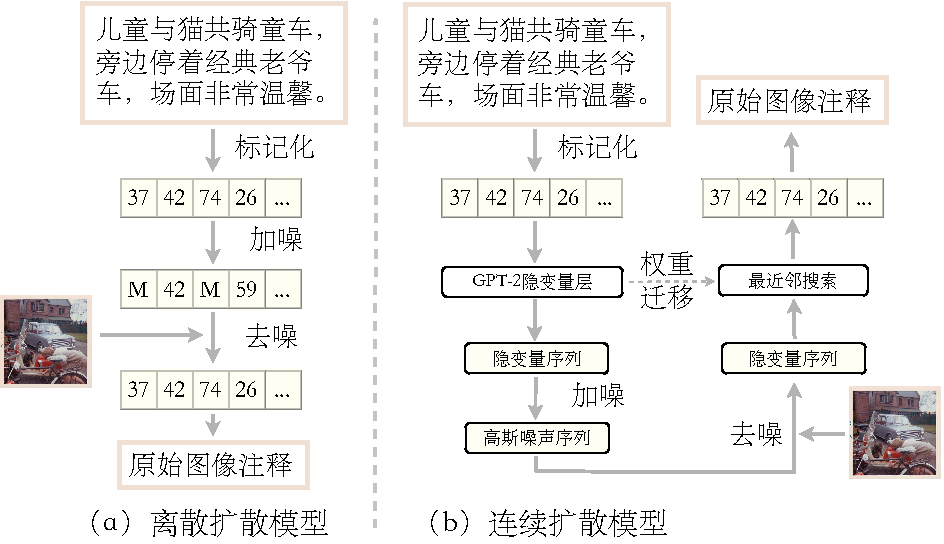
\includegraphics[width=0.8\linewidth]{figures/ddcap-cmp-continuous.pdf}
  \caption{文本生成离散扩散模型与连续扩散模型的建模方式对比}
  % image encoder; decoder (cross-attn) + time step
  \label{fig:ddcap-cmp-continuous}
\end{figure}

\subsection{与其他文本生成迁移方法的比较}
本节实验将离散扩散模型DDCap与连续扩散模型以及传统的自回归方法进行了比较。与连续扩散模型相比,离散扩散模型更符合文本信号特性,因此在图像描述生成任务中表现更优。而与传统的自回归方法相比,离散扩散模型允许对上下文同时进行建模,也可以取得相对更佳的表现。引入两阶段训练过程后,DDCap方法在图像描述生成任务中可以达到与一些大规模自回归生成方法相当的表现,并显著优于已有的非自回归方法。

\paragraph{与连续扩散模型和自回归方法的对比} 
本节实验设置与第\ref{sec:ddcap-exp-abl}节中的消融实验设置保持一致,只使用第二阶段数据进行训练和测试,并保证不同方法之间使用的生成模型参数量一致,以便公平比较。连续扩散模型和自回归方法的设置如下:
\begin{enumerate}
    \item 连续扩散模型用于文本生成任务的设计受图像生成领域中隐变量扩散模型\cite{latentdiff}启发。隐变量扩散模型本质是利用一个已训练好的隐变量提取器将连续或离散的输入信号转化为连续的隐变量,然后应用连续扩散模型进行建模。
    将该思想应用于文本生成任务时,本实验利用GPT-2预训练模型作为隐变量提取器,把离散的文本标记序列转换成连续的隐变量序列,并使用高斯噪声进行加噪过程。连续扩散模型的训练目标是基于加噪后的隐变量序列预测原始隐变量序列,再利用GPT-2预训练模型通过最近邻搜索恢复出原始文本标记。整体流程如图\ref{fig:ddcap-cmp-continuous}所示。
    %总步长 T 的数目设置为 10,000,并且噪声计划是线性的。
    % 我们发现它有助于以下修改:1) 使用所有 em 的均值和方差归一化嵌入层层理向量;2) 在推理过程中,每个嵌入向量 $x_{t}$ 被解码为标记,然后重新嵌入到向量中,然后估计 $x_{t-1}$ 。
    \item 自回归方法的设置与通常做法类似:在给定CLIP视觉表征之上训练一个自回归解码器以实现文本生成任务,并和DDCap方法一致,通过交叉注意力的机制将视觉表征引入自回归解码器中。
\end{enumerate}

\begin{table}
  \centering
  \caption{DDCap方法与连续扩散模型和自回归方法的性能对比}
  \begin{tabular}{lccccc}
    \toprule
    方法  & C & B@4 & M & R & S\\
    \midrule
    自回归方法 & 112.8  & 33.9 & 28.0 & 56.4 & 21.3\\
    连续扩散模型 & 91.9 & 25.0 &25.0&51.1& 19.1 \\
    DDCap  & \textbf{117.8} & \textbf{35.0}  & \textbf{28.2} & \textbf{57.4} & \textbf{21.7}\\
    \bottomrule
  \end{tabular}
  \label{tab:ddcap-framecom}
\end{table}
% 将连续扩散模型的训练轮次加长到100个
实验结果如表\ref{tab:ddcap-framecom}所示。与连续扩散模型相比,离散扩散模型在图像描述生成任务上的表现明显更优。这是因为离散扩散模型利用了文本信号具有离散性、冗余性低等特点,所以更适合以文本生成为目标的图像描述生成任务。
与自回归方法相比,离散扩散模型的表现也更优。这可能是由于离散扩散模型模拟了人类写作过程中的修正策略,允许模型在推理过程中利用上下文信息对中间文本标记进行修改,因此避免了因固定生成顺序而导致的误差累积问题。

\paragraph{与大规模自回归方法和其他非自回归方法的对比} 参照大规模自回归方法的训练策略,本组实验在DDCap方法中引入了第一阶段的通用图文数据集进行训练,并在第二阶段中针对MSCOCO数据集进行微调。表\ref{tab:ddcap-compsota}展示了DDCap方法与大规模自回归方法和其他非自回归方法的比较结果。
% 其中标注了$^\dagger$的方法引入了额外的目标检测模型对视觉表征进行增强。% \todo{把这些数据单位统一下,没有的数字要确认} 特别是那些别的单位的
与其他非自回归方法相比,DDCap方法取得了最佳性能,表明了新方法的有效性。% 可能要看一下和之前非自回归方法的主要区别
与已有的大规模自回归方法相比,在训练图像数量相当的情况下,DDCap方法的图像描述生成性能已经优于许多已有方法,并与ViTCap\cite{ViTCap}方法表现相当。这一结果展现了利用离散扩散模型实现高质量语义生成任务迁移的潜力。


\begin{table}
  \centering
  \caption{DDCap方法与自回归方法和非自回归方法的性能对比}
  % \setlength\tabcolsep{3pt}
  \begin{tabular}{lcccccc}
    \toprule
    方法 & 参数量 & 训练图片数 & C & B@4 & M & S\\
    \midrule
    \multicolumn{7}{l}{\textbf{自回归方法}}\\
    \midrule
    $\rm{UVLP}$~\cite{zhou2020unified}  & 0.1B & 4M & 116.9 & 36.5 & 28.4 & 21.2 \\
    % $\rm{MiniVLM}$~\cite{wang2020minivlm}  & 34.5M & 14M & 119.8 &  35.6 & 28.6 & 21.6  \\
    % $\rm{DistillVLM}$~\cite{fang2021compressing}  & 34.5M & 7M & 120.8 &  35.6 & 28.7 & 22.1 \\
    $\rm{UFO_B}$~\cite{UFO} & 0.1B & 4M & 122.8 & 36.0 & 28.9 & 22.2 \\
    $\rm{OSCAR_B}$~\cite{OSCAR} & 0.2B & 7M & 123.7 & 36.5 & 30.3 & 23.1\\ 
    $\rm{UNIMO_B}$~\cite{UNIMO}  & 0.2B & 9M & 124.4 &  38.8 & - & - \\
    ViTCap~\cite{ViTCap} & 0.2B & 4M & 125.2 & 36.3 & 29.3 &  22.6 \\
    $\rm{VinVL_B}$~\cite{VinVL} &  0.3B & 6M & 129.3 & 38.2 & 30.3 & 23.6\\ 
    $\rm{GIT_B}$~\cite{GIT} & 0.1B & 4M & 131.4 & 40.4 & 30.0 & 23.0 \\
    $\rm{LEMON_B}$~\cite{LEMON}& 0.1B & 200M& 133.3& 40.3& 30.2& 23.3\\
    $\rm{SimVLM_B}$~\cite{SimVLM}& -& 1800M & 134.8& 39.0& 32.9& 24.0\\ 
    % $\rm{OFA_B}$~\cite{wang2022ofa} & 184M & 4M & 138.2 & 41.0 & 30.9 & 24.2 \\
    \midrule
    \multicolumn{7}{l}{\textbf{非自回归方法}}\\
    \midrule
        $\rm{MNIC}$~\cite{gao2019masked}  & -  & - & 108.5 & 31.5 & 27.5 & 21.1\\
    $\rm{NAIC_{B,KD}}$~\cite{guo2020non}  & -  & - & 115.5 & 35.3 & 27.3 & 20.8\\
        $\rm{FNIC}$~\cite{fei2019fast}  & -  & - & 115.7 & 36.2 & 27.1 & 20.2\\
            $\rm{DDCap}$  & 0.3B & 4M & \textbf{125.1} & \textbf{37.1} & \textbf{29.1} & \textbf{22.7}\\
    % \hline  
    % $\rm{LEMON_L}$~\cite{hu2022scaling} & 338.3M & 0.2B & 135.7 & 40.6 & 30.4 & 23.5\\
    % $\rm{SimVLM_L}$~\cite{wang2021simvlm} & - & 1.8B & 142.6 & 40.3 & 33.4 & 24.7\\ 
    % $\rm{OSCARB_L}$~\cite{li2020oscar} & 0.3B+64M & 4M & 127.8 & 37.4 & 30.7  & 23.5\\ 
    % $\rm{VinVL_L}$~\cite{zhang2021vinvl} &  0.3B+0.2B & 6M & 130.8 & 38.5 & 30.4 &  23.4\\ 
    % $\rm{UFO_L}$~\cite{wang2021ufo} & 0.3B & 4M & 131.2 & 38.7 0 & 30.0 & 23.3 \\
    % $\rm{GIT_L}$~\cite{wang2022git} & 0.3B & 14M & 138.5 & 42.0 & 30.8 & 23.8 \\
    % $\rm{OFA_L}$~\cite{wang2022ofa} & 472M & 4M & 142.2 & 42.4 & 31.5 & 24.5 \\  
    % mPLUG~\cite{li2022mplug} & 0.6B & 14M & 141.0 & 43.1 & 31.4 & 24.2 \\
    \bottomrule
  \end{tabular}
%   \caption{Performance comparison on COCO captioning Karpathy~\cite{Karpathy2017DeepVA} split with pretraining, where B@4, M, R, C denote BLEU@4, METEOR, ROUGE-L,
% CIDEr and SPICE scores. CIDEr optimization is not used for all models. ($\dagger$) VinVL/OSCAR: the extra parameters are for
% object detector. All of the results do not contain CIDEr optimization.}
  \label{tab:ddcap-compsota}
\end{table}

% 可以把FD-CLIP的结果也放进来(from zixin)
% ckpt:https://vlpretraineastus.blob.core.windows.net/exp/output/simmlim/simmim_pretrain_clipfeat_nomask_SmoothL1_afterln_3e_4__vit_base__img224__300ep_crop008_dp02/ckpt_epoch_299.pth
% 不过实验设置对得不是很齐(pre-train 15ep,哦,我们也是pt15m,只是没有ft)而且只测了C,没测其他,可能还有些别的设置不太一样
% baseline是124.42,fd之后是126.43,384是127.388

\subsection{图像描述修改任务与模型定性分析}

\begin{figure}
  \centering
  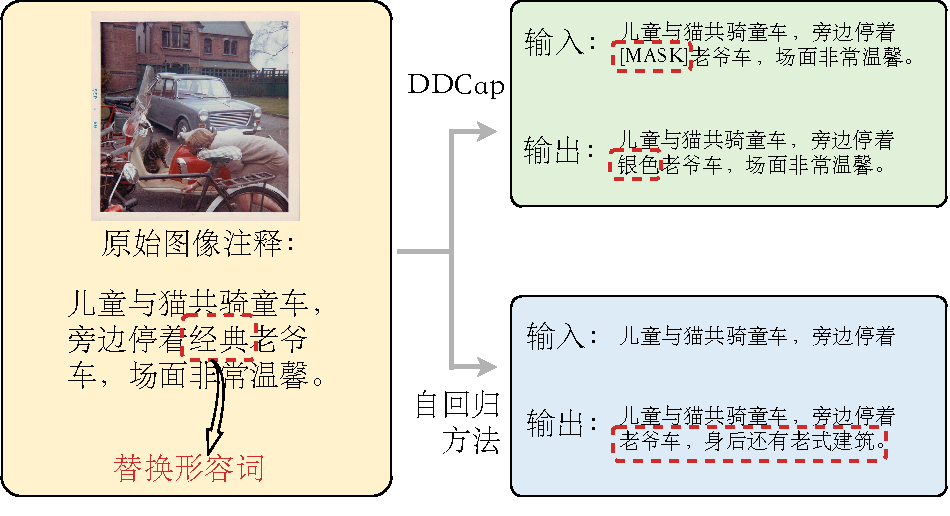
\includegraphics[width=0.8\linewidth]{figures/ddcap-modification-task.pdf}
  \caption{考虑人机互动场景的图像描述修改任务示意图}
  % image encoder; decoder (cross-attn) + time step
  \label{fig:ddcap-modification-task}
\end{figure}

\paragraph{DDCap方法在图像描述修改任务中的表现}
由于DDCap方法是一种并行生成方法,文本标记不是从左到右按固定顺序进行生成。因此此类方法有利于处理需要对图像描述进行填充或修改的任务。
如图\ref{fig:ddcap-modification-task}所示,本节考虑了一种人机交互的应用场景,在该场景中模型需要针对人类反馈对图像描述进行修改。具体而言,该任务模拟了用户要求模型修改已生成图像描述中的形容词并返回一条新的图像描述的场景。% 本组实验通过筛选出图像注释中含有形容词的所有测试样本,并将其中的形容词去除,要求模型重新生成。

\begin{table}
  \centering
  \caption{DDCap方法和自回归方法在图像描述修改任务上的对比实验}
  \begin{tabular}{lcccccc}
    \toprule
    方法 & C & B@4 & M & R & S & CLIP-Score\\
    \midrule
    自回归方法 & 203.5 & 76.3  & 49.3 &89.1& 36.5 & 75.7\\
    DDCap & \textbf{230.3} & \textbf{85.1}  &  \textbf{56.3} & \textbf{93.1} & \textbf{39.9} & \textbf{76.4}\\
    \bottomrule
  \end{tabular}
  \label{tab:ddcap-infill}
\end{table}

表\ref{tab:ddcap-infill}展示了DDCap方法与自回归方法在图像描述修改任务上的性能比较。由于DDCap方法是一种并行生成方法,它在生成当前文本标记时能够同时考虑前文和后文。不同于自回归方法,DDCap方法可以完全保留后文而不需要重新生成。因此,DDCap方法在比较图像描述修改前后的单词匹配度、公共子序列长度等测试指标上更有优势。
为了进一步评估修改后图像描述与图像的匹配程度,本组实验引入了CLIPScore\cite{CLIPScore}指标。该指标利用CLIP模型对齐视觉表征和语言表征的能力,可以有效评估修改后图像描述与图像间的语义关系,建模单个形容词改动带来的细微语义变化。从结果来看,DDCap方法相比于自回归方法在此类图像描述修改任务上效果更佳。


\begin{figure}
  \centering
  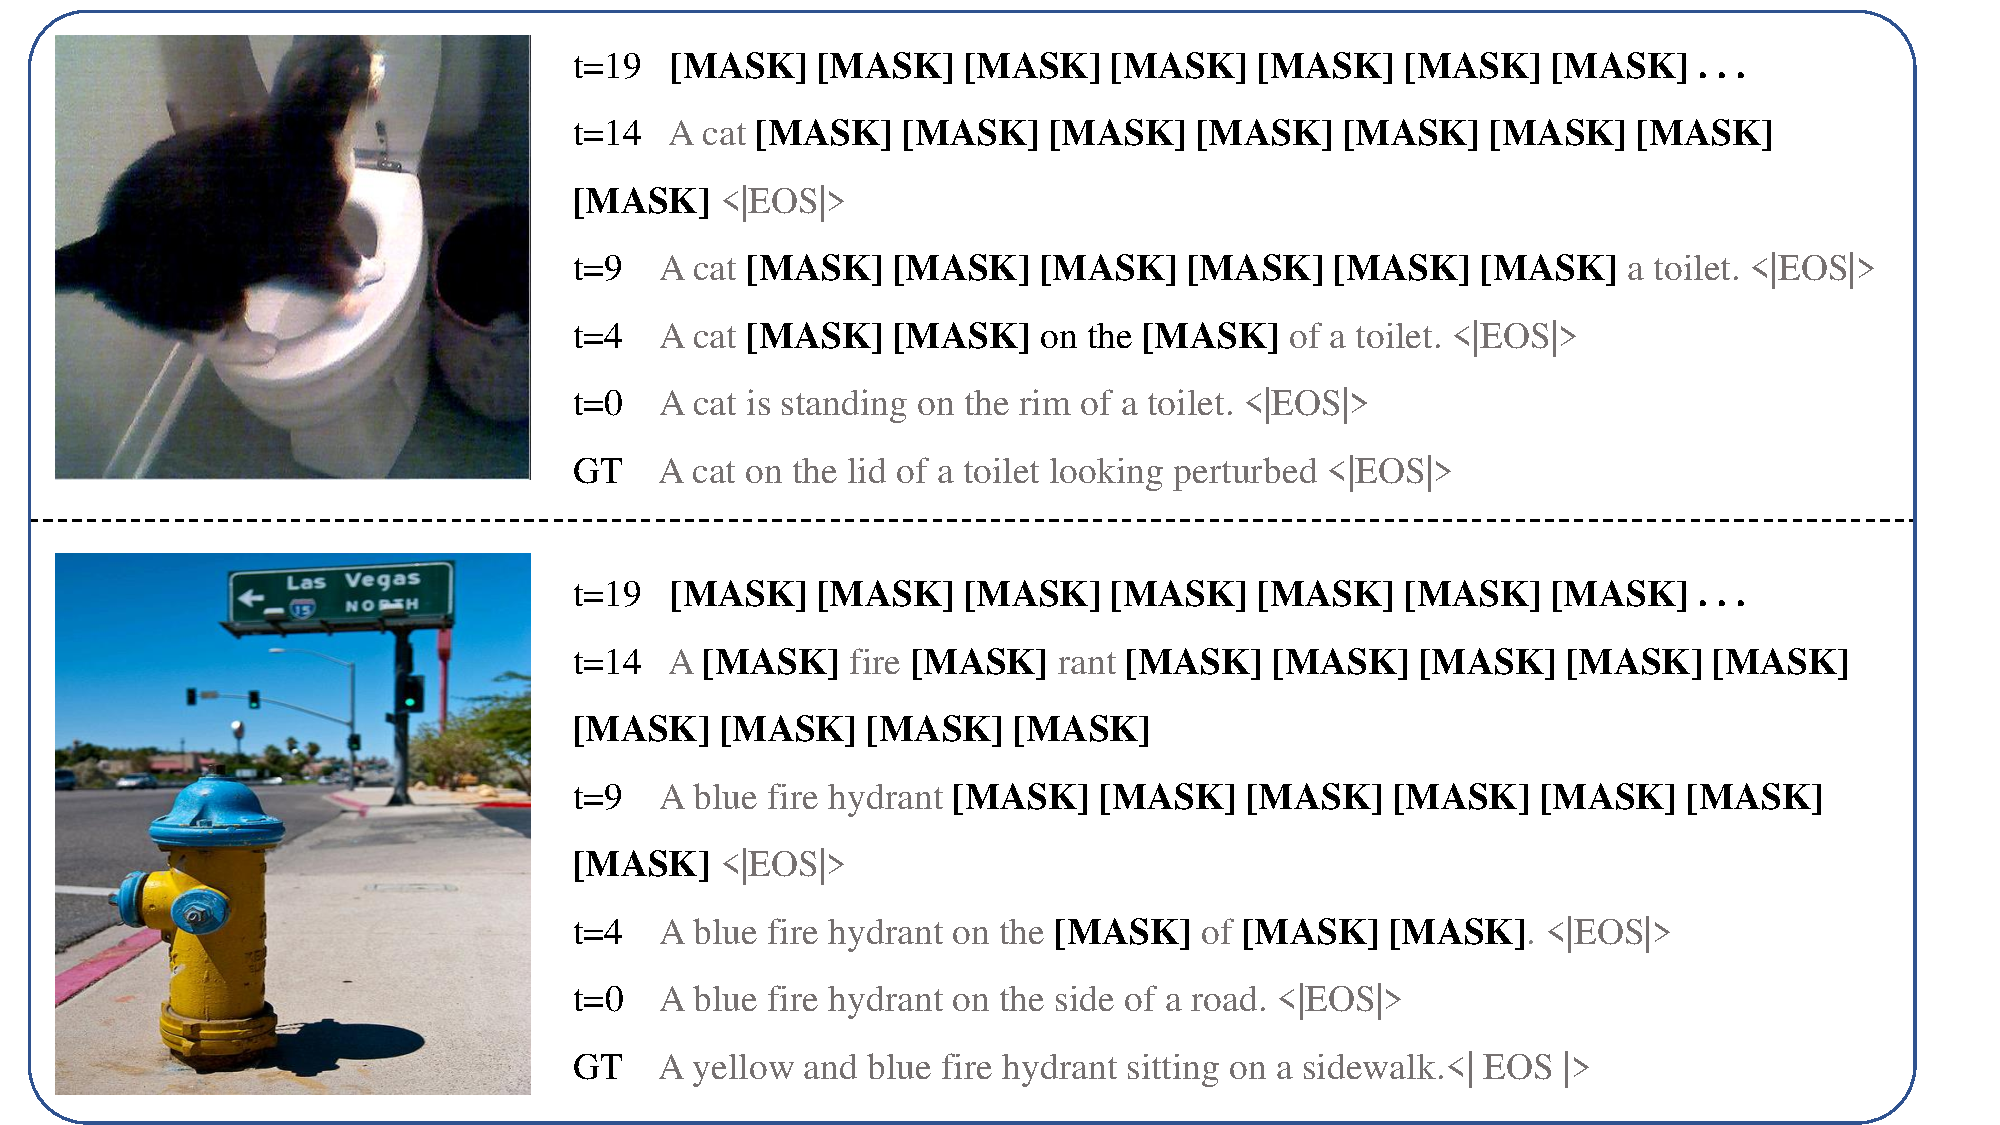
\includegraphics[width=1.0\linewidth]{figures/ddcap-generate-order.pdf}
  \caption{DDCap方法生成图像描述过程的可视化}
  % image encoder; decoder (cross-attn) + time step
  \label{fig:ddcap-generate-order}
\end{figure}

\begin{figure}
  \centering
  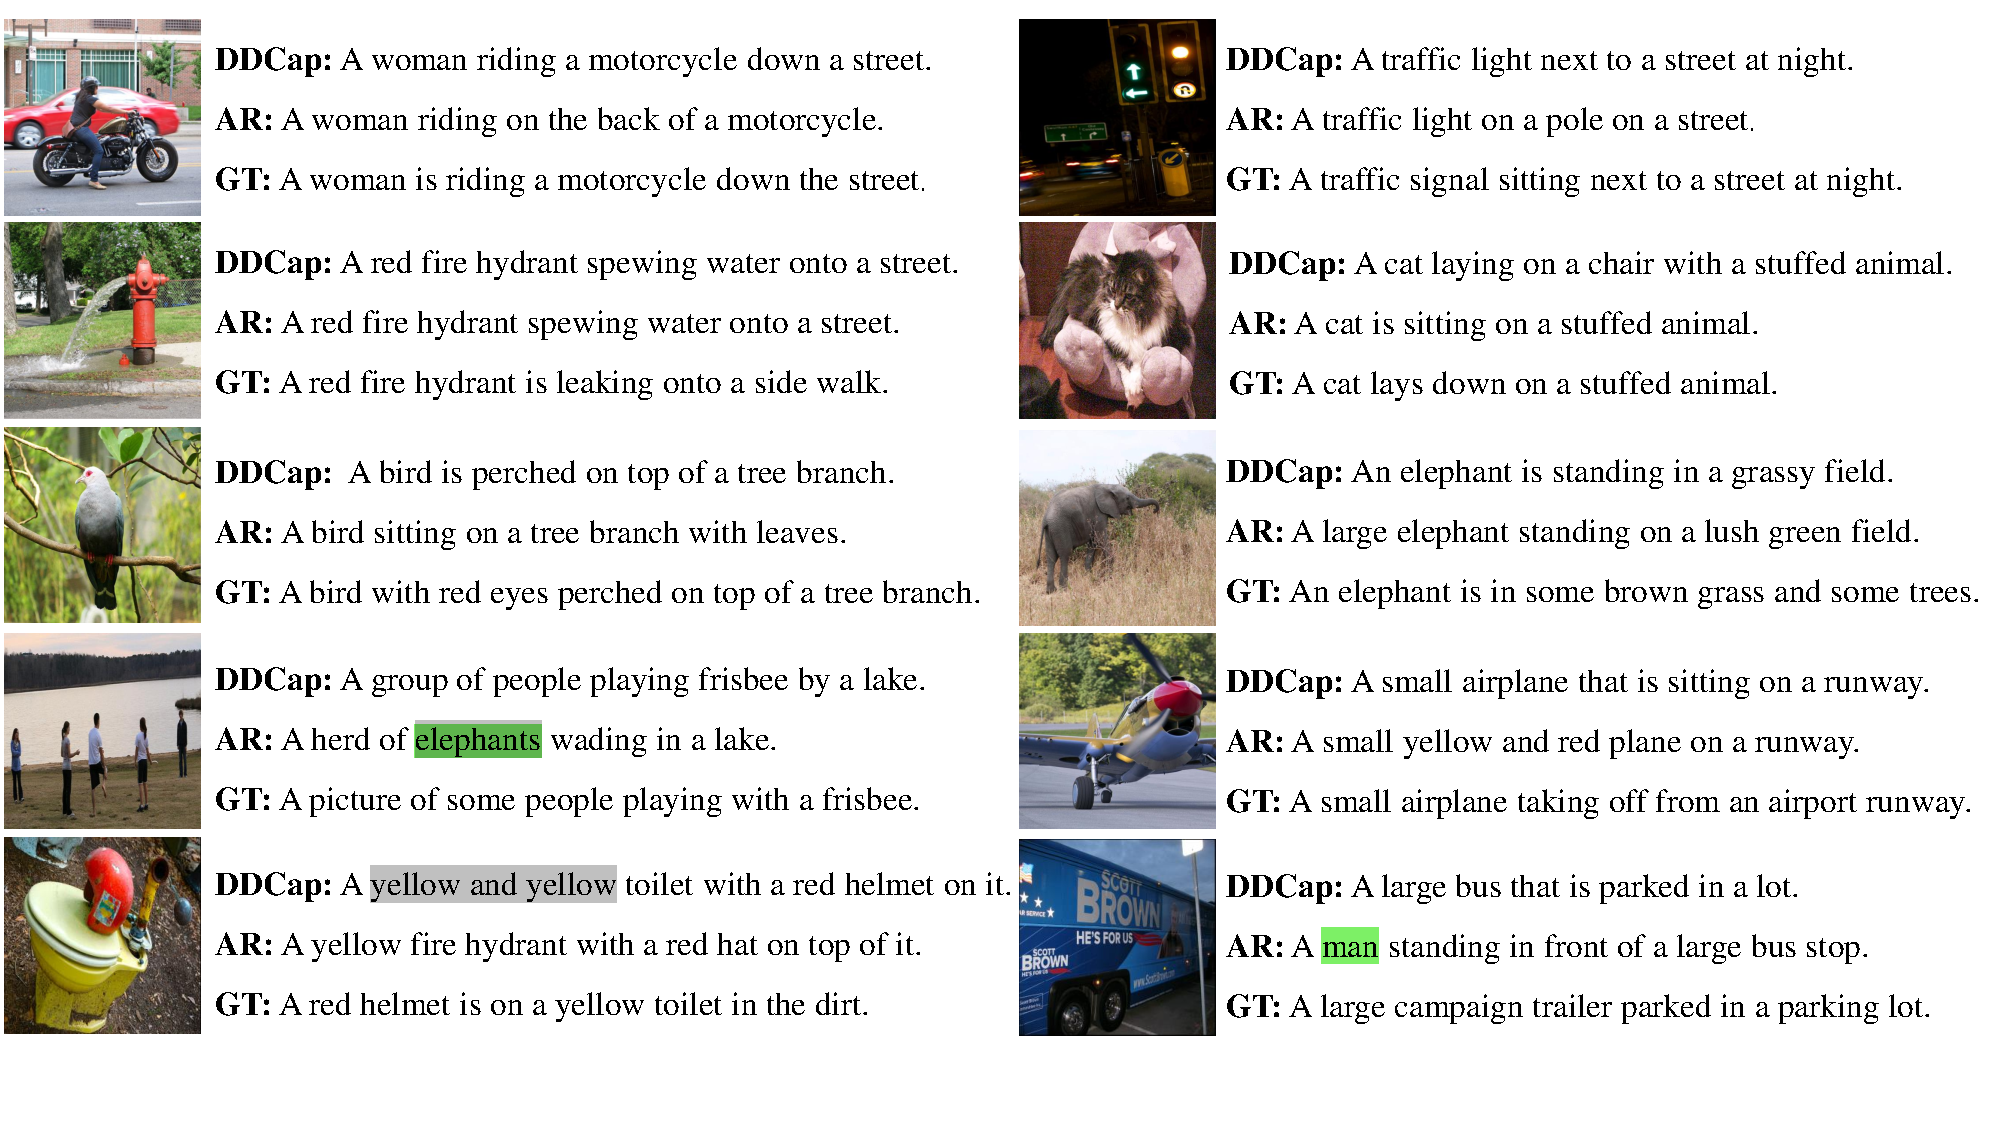
\includegraphics[width=1.0\linewidth]{figures/ddcap-qualification.pdf}
  \caption{DDCap方法与自回归方法的图像描述生成结果可视化}
  % image encoder; decoder (cross-attn) + time step
  \label{fig:ddcap-qualification}
\end{figure}


\paragraph{模型定性分析} 图\ref{fig:ddcap-generate-order}以MSCOCO测试集中的部分图像为例,展示了DDCap方法生成图像描述的顺序。通过观察模型的行为,可以得出如下结论:DDCap方法通常首先生成图像中的主体对象和对应的冠词,接着生成表示主体对象间相对关系的介词以及描述这些对象的形容词,最后生成其他名词、动词等使得句子语法正确。这一过程与人类自然思维顺序有一定相似性,展现了从点到线再到面的生成逻辑。

此外,图\ref{fig:ddcap-qualification}展示了DDCap方法和自回归方法在MSCOCO测试集部分样例上的图像描述生成结果,其中“AR”表示自回归方法生成的图像描述,而“GT”表示数据集中的参考描述。图中灰色块展示了部分生成结果的错误之处。相比于自回归方法,DDCap方法在识别图像中的主体对象方面表现更优。但由于DDCap方法依赖长度预测任务,且如图\ref{fig:ddcap-length}所示,长度预测误差存在较明显的分布倾向,也即预测序列长度比实际序列长度略长的概率更大。因此,当图像描述序列的长度预测结果更长,与实际长度有较大偏差时,DDCap方法生成的图像描述存在利用重复内容填充给定序列长度的现象。
% 但是,我们的 DDCap 有时会生成一些重复的单词。这个问题可以通过两种方式处理:(i) 我们首先获取标题,然后找到这些重复的单词。这些重复的单词将被重新屏蔽和重新生成。(ii) 标题中重复的单词将被删除。然后我们得到这个标题的新长度,没有重复的单词。根据新的长度,我们重新生成整个标题。

\section{总结}
\label{sec:ddcap-summary}
% \todo{怎么都没有提并行生成加速的事情?那前面里离散的motivation也别提了。}

% 因此,本文的贡献总结为
% • 我们是第一个将离散扩散模型应用于图像描述的公司,并提供了第一个证据,证明扩散模型可以达到与最好的、完善的自回归模型相比的竞争性能。
% • 我们提出了四个关键设计:(i) 长度预测用于处理文本生成中的可变长度问题;(ii) 集中注意力掩码用于提取紧凑的文本信息,而不会受到不需要的噪音的干扰;(iii) 提出了最佳优先推理以减少污染正确生成的令牌的机会;(iiii) 无图像训练,以平衡文本先验和图像条件中的信息。
% • 我们进一步展示了离散扩散模型在标题填充任务中的优势。

% 背景+motivation
语言-图像对比学习方法通过大规模互联网图文数据对训练,实现了视觉表征与语言表征的有效对齐。CLIP方法不仅增强了视觉表征的零样本泛化能力和下游视觉任务的迁移效果,还构建了多模态共享的联合表征空间,显著提高了跨模态转化效率。本章重点探讨了基于CLIP视觉表征的语义生成任务迁移方法。
% 对齐了视觉表征和语言表征。CLIP方法在增强了视觉表征的零样本泛化性和下游视觉任务迁移效果的同时,构建了两种模态共享的表征空间,极大地提升了不同模态间的转化效率。
% Dall-E 2的工作正是利用了CLIP方法搭建的跨模态桥梁,实现语言表征向视觉表征的映射,以完成基于文本的图像生成任务。受Dall-E 2的启发,
% 本章讨论了基于CLIP视觉表征实现语义生成任务的迁移方法设计。

% 解决方案和发现
受到扩散模型在图像生成任务中成功应用的启发,本章讨论了扩散模型作为图像描述生成任务迁移方法的可行性。直接将针对图像生成任务设计的扩散模型应用到文本生成任务上存在诸多问题,因此本章分析了文本信号区别于图像信号的关键特性:离散性、低冗余性、序列长度可变性。基于这些分析,本章提出了DDCap方法,通过集中注意力掩码模块、长度预测任务和最佳优先推理策略有针对性地适配文本信号特点。
% 针对文本信号离散性的特点,本章以离散扩散模型为出发点,利用不同文本标记之间的转移和作为占位符的掩码标记[\texttt{MASK}]来代替针对连续信号设计的高斯噪声。在训练过程中考虑到文本信号的变长特性,本章引入待生成注释长度预测任务,以灵活地适应不同长度的文本。同时考虑到文本信息的低冗余性,以及由标记离散性导致的噪声强度不连续性,本章提出一个集中注意力掩码模块,以引导模型关注信息密度更高的标记。
% 在推理过程设计中同样考虑了低冗余性的特点,使用一种称为最佳优先推理的策略,在每一步中保留模型置信度最高的一些标记,并只对其他标记进行重新加噪后重新生成。此外,本章还将图像生成方法中的无分类器引导思想引入文本生成任务中。该方法在训练过程中随机丢弃图像输入,以达到强制模型学习语言建模的先验知识。
% 结果
实验证明了离散扩散模型在图像描述生成任务中的有效性。与其他并行生成方法相比,DDCap方法显著缩小了与主流自回归方法间的性能差距,并在需要人机交互的图像描述修改场景中展现出独特优势。

% 针对扩散模型在图像描述生成任务中的应用,本章分析了文本信号区别于图像信号的关键特性:离散性、低冗余性和变长特性。基于这些分析,本章提出了DDCap方法,并通过实验证明了离散扩散模型在图像描述生成任务中的有效性。与其他并行生成方法相比,DDCap方法显著缩小了与主流自回归模型间的性能差距,并在需要人机交互的图像描述修改场景中展现出独特优势。

% 总结前三章工作
结合本章工作与前序两章工作,本文系统性地探讨了CLIP方法的视觉表征预训练策略和下游任务迁移方法,包括利用高质量标注的图像分类数据增强CLIP视觉表征泛化性和语义准确度、通过特征图自蒸馏提升CLIP方法细粒度视觉任务的迁移效果、以及基于离散扩散模型实现CLIP方法向语义生成任务迁移的方法。这一系列工作全面提升了CLIP方法在多种视觉和多模态任务中的应用能力。

% 结合前两章工作,本研究系统性地探讨了CLIP方法的预训练策略和下游任务迁移技术,包括利用高质量标注数据增强视觉表征泛化性、通过特征图自蒸馏提升细粒度视觉任务的迁移效果,以及基于离散扩散模型实现语义生成任务的迁移方法。这一系列工作全面提升了CLIP模型在多种视觉和跨模态任务中的应用能力。
% !TeX root = ../main.tex
\chapter{总结与展望}
\label{cha:summary}
\section{本文总结}
“预训练-微调”范式作为数据驱动的深度学习方法的重要范式,在计算机视觉和自然语言处理领域取得了显著成功。该范式通过解耦通用表征学习与下游任务迁移两个阶段,利用大规模预训练数据缓解下游任务数据标注困难的问题,从而提升了模型迁移性能。视觉任务的核心挑战在于实现从像素级感知特征到语义级认知概念的有效映射。传统的视觉预训练方法各有局限:有监督图像分类方法受限于封闭的类别语义空间和数据扩展性,而自监督方法则停留在感知特征层面,无法获取语义知识。语言-图像对比学习(CLIP)方法借助语言模态在语义表达上的优势,通过大规模互联网图文数据对为开放语义的视觉表征学习提供了有效解决方案。然而,CLIP方法仍面临着预训练数据的语义噪声、细粒度视觉任务的迁移效果欠佳以及缺乏语义生成能力等方面的挑战。针对这些问题,本文提出了一系列创新性解决方案,显著提升了模型在视觉表征学习和下游任务迁移两方面的效果。本文的主要创新成果为:

\begin{itemize}
    \item 针对互联网图文数据对中的语义信号噪声问题,\textit{提出基于高质量图像分类数据扩展的预训练方法。} 本文首先对比分析了互联网图文数据对的噪声特点与图像分类标注的高可区分性,提出利用高质量图像分类数据增强CLIP方法的视觉表征学习效果。通过从损失函数形式、分类器权重参数化方法、标注信息的语义丰富度三个维度分析了两种方法和数据的不同,本文提出从对比学习的视角重新构建图像分类任务的方法,实现了建模形式的统一,并引入分布式优化策略来处理类别数目较大的分类数据集。为进一步增强视觉表征的语义表达能力,本文引入外部专家知识库扩充类别标签的语义信息,实现了对两种数据源的有效融合利用。该方法在多个数据组合上得到验证,显著提升了模型在零样本开放集合图像识别和图文跨模态检索任务上的性能,证明了通过对比学习框架整合高质量视觉数据来增强CLIP方法视觉表征和语言表征对齐效果的有效性。
    \item 针对CLIP方法在细粒度视觉任务上迁移效果欠佳的问题,\textit{提出基于特征图自蒸馏增强的细粒度视觉任务迁移方法。} 尽管CLIP方法的视觉模型通过语言监督获得了丰富的语义表征,本文通过实验发现在需要密集预测能力的细粒度视觉任务上,CLIP方法的迁移能力不及基于像素级自监督的预训练方法。针对这一问题,本文从输入完整性、训练目标粒度和损失函数设计三个维度对比分析了两类预训练方法,揭示了像素级视觉训练目标对提升模型密集预测能力的关键作用。考虑到对互联网图文数据对进行像素级标注的巨大成本和重新预训练的计算开销,本文提出特征图自蒸馏方法。该方法利用CLIP模型的输出特征图作为自蒸馏目标得到训练学生模型:既引入了像素级视觉训练信号,又保留了原始模型中的语义信息。该方法得到的新模型在语义分割、目标检测、深度估计等细粒度视觉任务上显著提升了迁移性能。此外,特征图自蒸馏方法也被成功推广到其他视觉预训练模型,展现出良好的通用性。
    \item 针对CLIP方法缺乏直接完成语义生成任务的问题,\textit{提出基于离散扩散模型的语义生成任务迁移方法。} 与图像生成领域相比,将扩散模型应用于文本生成任务面临文本信号的离散性、低冗余性和序列长度可变性等挑战。基于这些特点,本文从离散扩散模型出发设计了适配的训练策略和推理机制,包括集中注意力掩码模块、长度预测任务和最佳优先推理策略。相比传统的自回归方法,基于扩散模型的语义生成迁移框架具有显著优势:能够同时利用上下文信息增强生成质量、支持对已生成内容的灵活修改。实验表明,该方法在图像描述生成任务上达到了与成熟自回归方法相当的性能,同时在需要交互式修改图像描述的场景中表现更出色,为CLIP方法在语义生成任务上的迁移开辟了新途径。
\end{itemize}

\section{未来工作展望}
本文针对CLIP方法在视觉表征学习以及下游任务迁移两个方面提出了创新性的解决方案。然而,随着语言-图像对比学习领域的快速发展,仍有许多值得深入探索的方向。未来的研究工作可以从以下几个方面展开:
% 增强可训练数据 - 工作一
\paragraph{从图文数据对到网页数据的CLIP训练方法}
CLIP方法的视觉表征学习效果很大程度上依赖于预训练数据的语义信息质量和多样性。虽然第\ref{cha:iclip}章探讨了利用高质量图像分类数据的增强方法,但当前从网页获取图文数据对的过程忽略了大量有价值的信息:网页正文往往包含更丰富的图像相关描述,而页面中的其他图像也与目标图像形成语义关联。因此,如何有效利用网页数据中更完整的语义信息进行预训练\cite{S4, NEURIPS2024_2a952768}成为一个重要研究方向。
该方向的关键挑战在于如何有效建模网页中多图多文的结构化信息。现有方法主要有两种思路:一是利用文档对象模型将网页元素组织为树结构,并转化为序列形式处理\cite{DomLM,layoutlm};二是采用图像形式保留网页的二维布局信息\cite{CLIPPO}。然而,这些方法或损失了空间结构信息,或降低了文本处理效率。因此,设计更优的网页数据建模方法将是未来研究的重点。

% 增强语言模型的性能 - 工作二
\paragraph{大语言模型赋能的CLIP训练方法}
% CLIP作为一种视觉-语言多模态联合预训练方法,对于视觉-语言交叉领域有重要意义。
尽管CLIP方法通过语言监督增强了视觉表征的语义理解能力,且第\ref{cha:fd}章进一步提升了其在细粒度视觉任务上的迁移表现,但研究表明\cite{bow,CLIPA}CLIP方法的语言模型不擅长处理复杂、长程和细微的语义关系。这主要源于图文数据对中的文本规模和知识密度远低于大语言模型的训练数据:后者的训练量通常是前者的数十倍到数百倍\cite{gpt4, dsv3, radford2021learning},且来源丰富性更好。
现有工作主要通过两种方式整合大语言模型的能力:一是将CLIP视觉表征接入大语言模型并进行联合微调\cite{blip-2, llava},二是利用大语言模型指导CLIP视觉表征学习\cite{LLM2CLIP}。然而,如何从预训练阶段就实现视觉和语言能力的深度融合,构建一个在两个模态上都具有卓越表现的统一模型\cite{gemini},将会是未来重要研究方向。

% 处理更复杂的多模态任务 - 工作三
\paragraph{时空信息与语言信息结合的训练方法}
目前CLIP方法只建模了图像与文本间的对应关系,这与人类在真实世界中的学习过程有显著差异。人类视觉系统不仅需要处理三维空间信息,还需要理解时序变化,通过持续的观察、交互和思考来建立对世界的认知。因此,如何扩展当前预训练框架,使其具备对空间几何和时序信息的建模能力,同时通过语言模态理解语义信息,将对具身智能和机器人应用具有重要意义。
% 近期提出的视觉语言导航\cite{vln}和视觉-空间智能评测\cite{VSIBench}等任务为这一方向提供了良好的验证平台。这些任务要求模型同时具备空间场景理解、语言指令解析和时序推理能力。然而,如何设计合适的预训练方法来获取这些能力仍是一个开放问题。
% 正如ImageNet数据集\cite{deng2009imagenet}推动了视觉模型发展,Conceptual Captions\cite{sharma-etal-2018-conceptual,changpinyo2021conceptual}促进了视觉-语言预训练,Common Crawl\cite{cc,pile}加速了大语言模型进步
数据驱动是深度学习方法的重要思想。获取高质量的时空-语言对齐数据是该领域的关键挑战。与易于获取的图文数据对不同,包含空间信息的真实场景数据采集成本高昂且规模有限。近期生成式模型的突破\cite{latentdiff,veo2}为解决这一问题提供了新思路:通过可探索三维空间的生成办法\cite{genex, genie2},有望大规模合成高质量的时空-语言训练数据,为下一代训练方法开辟新途径。

% CLIP作为一种视觉-语言多模态训练方法,其本质是一种图像-文本多模态训练方法。但现实世界中的视觉信号形式丰富多样,图像信息只是其中一种。若将模型训练过程类比为一个刚出生的婴儿的学习过程,那么语言-图像对比学习方法的学习过程类似于完成图像与文字的连连看游戏。但人的视觉系统是三维的,同时人的活动是有时序性的。每一个婴儿都在三维空间中不断地观察、感知、交互、思考、行动,从而建立起对世界的认知和对语言的理解。这与当前语言-图像对比学习方法的训练过程大相径庭,也说明了语言-图像对比学习方法的局限性。如何得到一个既能够处理三维空间信息和时序信息,又能理解人类丰富语言信息的视觉-语言多模态训练方法将是未来的一个重要方向,对于具身智能和机器人应用有重要意义。

% 最近提出的视觉语言导航\cite{vln}任务就是一类很好的评测方法。这类任务考验了模型在三维世界里观察环境的能力,同时需要模型对语言指示有足够的理解能力,并在时序上基于过去信息进行推理和规划。与之类似的还有视觉-空间智能评测任务\cite{VSIBench},这类任务要求模型对一段给定视频里的空间场景进行理解和记忆,并针对以自然语言给出的问题进行推理和回答。虽然最近的研究工作在评测方法设计上有较多进展,但如何进一步扩展语言-图像对比学习方法,使其具备对几何空间和时序信息的建模能力还不清楚。

% 数据驱动性是深度学习领域的重要思想,所以数据往往被视为优先事项。ImageNet数据集\cite{deng2009imagenet}的出现推动了有监督视觉模型的繁荣。以Conceptual Captions\cite{sharma-etal-2018-conceptual,changpinyo2021conceptual}为例的数据集出现,推动了语言-图像对比学习方法的研究。Common Crawl\cite{cc,pile}等互联网级文本数据的出现推进了大语言模型的发展。如何构造时空信息与语言信息对齐的训练数据是该方向最本质的问题。与图文数据对不同,虽然互联网上有很多包含时序信息的视频数据可以作为训练数据,但空间信息很少以电子化的方式存在,而且在现实场景中采集这样的信息成本又较高,因此这种训练数据的规模较小,不足以支撑模型预训练。得益于生成式内容的技术发展\cite{latentdiff,veo2},越来越多的研究工作开始设计可探索三维空间的生成办法\cite{genex, genie2}。这些生成式模型的出现为大规模、低成本合成时空信息与语言信息结合的训练数据提供了新的可能性,也为未来研究提供了新的方向。

% 其他部分
\backmatter

% 参考文献
\bibliography{ref/refs}  % 参考文献使用 BibTeX 编译
% \printbibliography       % 参考文献使用 BibLaTeX 编译

% 附录
% 本科生需要将附录放到声明之后,个人简历之前
\appendix
% \input{data/appendix-survey}       % 本科生:外文资料的调研阅读报告
% \input{data/appendix-translation}  % 本科生:外文资料的书面翻译
% \input{data/appendix}

% 致谢
% !TeX root = ../main.tex

\begin{acknowledgements}
  时光荏苒,五年博士生涯如白驹过隙。回顾这五年科研时光,是各位老师、朋友、家人的关心与支持一路陪伴我走到现在。在此之际,铭以致谢。

  % 首先,我要衷心感谢我的导师郭百宁老师。郭老师知识渊博、幽默风趣、温和谦逊,有大师风范。
  % 作为微软亚洲研究院的副院长,他熟稔科技的发展和行业的进步,在我的科研项目中提出宝贵的指导意见,也在我的人生选择中为我指出一条明路。
  % 这五年时间里,他为我创造了自由、灵活的良好环境,鼓励我和微软亚洲研究院的各位老师交流学习,也支持我勇敢追求自己兴趣所在。
  % 郭老师的言行品格和谆谆教诲将一直在未来人生道路上警醒我、激励我向远方的未知探索。

  首先,我要衷心感谢我的导师\textit{导师隐名}。\textit{导师隐名}知识渊博、幽默风趣、温和谦逊,有大师风范。
  他熟悉科技的发展和行业的进步,在我的科研项目中提出宝贵的指导意见,也在我的人生选择中为我指出一条明路。
  这五年时间里,他为我创造了自由、灵活的良好环境,鼓励我和微软亚洲研究院的各位老师交流学习,也支持我勇敢追求自己兴趣所在。
  \textit{导师隐名}的言行品格和谆谆教诲将一直在未来人生道路上指引我、激励我向远方的未知探索。
  
  其次,我要衷心感谢在微软亚洲研究院联合培养期间给予我指导的每一位研究员,是他们教会了我科研的方法、梳理问题的逻辑和展示自我的能力。
  感谢曹越博士从最基础的科研方法和科研工具开始,帮助我、引导我一步一步走上科研的道路,他对问题的深刻认知让我受益匪浅。
  感谢胡瀚博士一直以来的引领和鼓励,在我迷茫的时候指引我、在我受挫的时候激励我、在我无措的时候教导我,他对问题核心的精准把握值得我终身学习。
  感谢张拯博士和彭厚文博士的言传身教,让我不断提升自我,不断进步。

  我也要感谢在微软亚洲研究院期间合作过和给予我帮助的每一位研究员:童欣博士、Stephen Lin 博士、戴琦博士、王春雨博士、鲍建敏博士、元玉惠博士、陈栋博士、陈鹏博士、董悦博士、刘自成博士、Jianfeng Wang 博士、杨一帆老师、李骥老师。
  也要感谢姚朱亮师兄、唐彦嵩师兄、徐孟德师兄,祝愿他们事业有成、勇攀高峰。
  还要感谢一起合作过同学,张淼森、李睿航、李晨、宁嘉、耿子刚、尼博林、吴侃、朱子欣、王瑞哲、黄伟泉,祝愿他们学习有成、科研顺利。
  更要感谢解振达、刘泽、林宇桐、胡倞成,与他们的深厚友谊一直支持我,祝他们得偿所愿。

  我的成长也离不开母校的关心和关怀。感谢高等研究院的李丽老师、姜久红老师和王亮老师的支持,也感谢高研博党支部的各位同志的鼓励,感谢支书黄泰榕和支委刘铄、孔舒婷的默默付出,感谢我的室友王颢琛和郑欣阳的陪伴。

  最后,我要感谢我的父母和家人,是他们无私的爱与支持和温暖的怀抱,成为我生命力量的源泉,鼓励我勇攀高峰,祝他们身体健康、心想事成。更要感谢我的爱人单昕霞,在十多年无数个难眠的夜里,给予我坚持的信心和直面自我的勇气。

  二十余载求学路,今日毕、八十余载求知路,方启航。在这个波澜壮阔的时代,衷心地祝愿每一个人都朝着自己的北斗星,扬帆起航。
  
  
\end{acknowledgements}


% 声明
% 本科生开题报告不需要
% \statement[page-style=empty]  % 编译生成的声明页默认不含页眉页脚
% \statement[page-style=empty, file=scan-statement-104.pdf]
% 插入签字后的扫描件 scan-statement.pdf,并添加页眉页脚
\statement[page-style=plain, file=scan-statement.pdf]

% 个人简历、在学期间完成的相关学术成果
% 本科生可以附个人简历,也可以不附个人简历
% !TeX root = ../main.tex

\begin{resume}

  \section*{个人简历}

  1998 年 8 月 28 日出生于浙江省东阳市。

  2016 年 9 月考入清华大学自动化系自动化专业,2020 年 7 月本科毕业并获得工学学士学位。

  2020 年 9 月免试进入清华大学高等研究院攻读计算机科学与技术专业博士学位至今。


  \section*{在学期间完成的相关学术成果}

  \subsection*{学术论文($^\ddag$表示共同作者)}

  \begin{achievements}
      \item \textbf{Wei Y}, Cao Y, Zhang Z, et al. iCLIP: Bridging Image Classification and Contrastive Language-Image Pre-training for Visual Recognition[C]//Proceedings of the IEEE/CVF Conference on Computer Vision and Pattern Recognition, 2023: 2776-2786. (TH-CPL 推荐 A 类会议)
    \item \textbf{Wei Y}, Hu H, Xie Z, et al. Improving CLIP Fine-tuning Performance[C]//Proceedings of the IEEE/CVF International Conference on Computer Vision, 2023: 5439-5449. (TH-CPL 推荐 A 类会议)
    \item Zhu Z$^\ddag$, \textbf{Wei Y}$^\ddag$, Wang J, et al. Exploring Discrete Diffusion Models for Image Captioning[A/OL]. 2022. arXiv: 2211.11694. https://arxiv.org/abs/2211.11694.
    % \item Ze Liu$^\ddag$, Yutong Lin$^\ddag$, Yue Cao$^\ddag$, Han Hu$^\ddag$, \textbf{Yixuan Wei}, Zheng Zhang, Stephen Lin, and Baining Guo: Swin transformer: Hierarchical vision transformer using shifted windows[C]//Proceedings of the IEEE/CVF International Conference on Computer Vision (ICCV), 2021: 10012-10022. (TH-CPL 推荐 A 类会议)
    % \item Ze Liu$^\ddag$, Jia Ning$^\ddag$, Yue Cao, \textbf{Yixuan Wei}, Zheng Zhang, Stephen Lin, and Han Hu: Video swin transformer[C]//Proceedings of the IEEE/CVF Conference on Computer Vision and Pattern Recognition (CVPR), 2022: 3202-3211. (TH-CPL 推荐 A 类会议)
    % \item Ze Liu$^\ddag$, Han Hu$^\ddag$, Yutong Lin, Zhuliang Yao, Zhenda Xie, \textbf{Yixuan Wei}, Jia Ning, Yue Cao, Zheng Zhang, Li Dong, Furu Wei, and Baining Guo: Swin transformer v2: Scaling up capacity and resolution[C]//Proceedings of the IEEE/CVF Conference on Computer Vision and Pattern Recognition (CVPR), 2022: 12009-12019. (TH-CPL 推荐 A 类会议)
    \item Yang Y$^\ddag$, Huang W$^\ddag$, \textbf{Wei Y}, et al. Attentive Mask Clip[C]//Proceedings of the IEEE/CVF International Conference on Computer Vision, 2023: 2771-2781. (TH-CPL 推荐 A 类会议)
    \item Geng Z, Wang C, \textbf{Wei Y}, et al. Human Pose As Compositional Tokens[C]//Proceedings of the IEEE/CVF Conference on Computer Vision and Pattern Recognition, 2023: 660-671. (TH-CPL 推荐 A 类会议)
    % \item Zhenda Xie, Zheng Zhang, Yue Cao, Yutong Lin, \textbf{Yixuan Wei}, Qi Dai, and Han Hu: On data scaling in masked image modeling[C]//Proceedings of the IEEE/CVF Conference on Computer Vision and Pattern Recognition (CVPR), 2023: 10365-10374. (TH-CPL 推荐 A 类会议)
    \item Li R, \textbf{Wei Y}, Zhang M, et al. ScalingFilter: Assessing Data Quality through Inverse Utilization of Scaling Laws[C]//Proceedings of the 2024 Conference on Empirical Methods in Natural Language Processing, 2024: 3209-3222. (TH-CPL 推荐 A 类会议)
    \item Zhang M, \textbf{Wei Y}, Xing Z, et al. Aligning Vision Models with Human Aesthetics in Retrieval: Benchmarks and Algorithms[J]. Advances in Neural Information Processing Systems, 2024, 37. (TH-CPL 推荐 A 类会议)  % 为啥这里写推荐会议但用的J

    
    % \item \textbf{Yixuan Wei}, Yue Cao, Zheng Zhang, Houwen Peng, Zhuliang Yao, Zhenda Xie, Han Hu, and Baining Guo: iclip: Bridging image classification and contrastive language-image pre-training for visual recognition[C]//Proceedings of the IEEE/CVF Conference on Computer Vision and Pattern Recognition (CVPR), 2023: 2776-2786. (TH-CPL 推荐 A 类会议)
    % \item \textbf{Yixuan Wei}, Han Hu, Zhenda Xie, Ze Liu, Zheng Zhang, Yue Cao, Jianmin Bao, Dong Chen, and Baining Guo: Improving clip fine-tuning performance[C]//Proceedings of the IEEE/CVF International Conference on Computer Vision (ICCV), 2023: 5439-5449. (TH-CPL 推荐 A 类会议)
    % \item Zixin Zhu$^\ddag$, \textbf{Yixuan Wei}$^\ddag$, Jianfeng Wang, Zhe Gan, Zheng Zhang, Le Wang, Gang Hua, Lijuan Wang, Zicheng Liu, and Han Hu: Exploring discrete diffusion models for image captioning[A/OL]. 2022. arXiv: 2211.11694. https://arxiv.org/abs/2211.11694.
    % \item Ze Liu$^\ddag$, Yutong Lin$^\ddag$, Yue Cao$^\ddag$, Han Hu$^\ddag$, \textbf{Yixuan Wei}, Zheng Zhang, Stephen Lin, and Baining Guo: Swin transformer: Hierarchical vision transformer using shifted windows[C]//Proceedings of the IEEE/CVF International Conference on Computer Vision (ICCV), 2021: 10012-10022. (TH-CPL 推荐 A 类会议)
    % \item Ze Liu$^\ddag$, Jia Ning$^\ddag$, Yue Cao, \textbf{Yixuan Wei}, Zheng Zhang, Stephen Lin, and Han Hu: Video swin transformer[C]//Proceedings of the IEEE/CVF Conference on Computer Vision and Pattern Recognition (CVPR), 2022: 3202-3211. (TH-CPL 推荐 A 类会议)
    % \item Ze Liu$^\ddag$, Han Hu$^\ddag$, Yutong Lin, Zhuliang Yao, Zhenda Xie, \textbf{Yixuan Wei}, Jia Ning, Yue Cao, Zheng Zhang, Li Dong, Furu Wei, and Baining Guo: Swin transformer v2: Scaling up capacity and resolution[C]//Proceedings of the IEEE/CVF Conference on Computer Vision and Pattern Recognition (CVPR), 2022: 12009-12019. (TH-CPL 推荐 A 类会议)
    % \item Yifan Yang$^\ddag$, Weiquan Huang$^\ddag$, \textbf{Yixuan Wei}, Houwen Peng, Xinyang Jiang, Huiqiang Jiang, Fangyun Wei, Yin Wang, Han Hu, Lili Qiu, and Yuqing Yang: Attentive mask clip[C]//Proceedings of the IEEE/CVF International Conference on Computer Vision (ICCV), 2023: 2771-2781. (TH-CPL 推荐 A 类会议)
    % \item Zigang Geng, Chunyu Wang, \textbf{Yixuan Wei}, Ze Liu, Houqiang Li, and Han Hu: Human pose as compositional tokens[C]//Proceedings of the IEEE/CVF Conference on Computer Vision and Pattern Recognition (CVPR), 2023: 660-671. (TH-CPL 推荐 A 类会议)
    % \item Zhenda Xie, Zheng Zhang, Yue Cao, Yutong Lin, \textbf{Yixuan Wei}, Qi Dai, and Han Hu: On data scaling in masked image modeling[C]//Proceedings of the IEEE/CVF Conference on Computer Vision and Pattern Recognition (CVPR), 2023: 10365-10374. (TH-CPL 推荐 A 类会议)
    % \item Ruihang Li, \textbf{Yixuan Wei}, Miaosen Zhang, Nenghai Yu, Han Hu, and Houwen Peng: ScalingFilter: Assessing Data Quality through Inverse Utilization of Scaling Laws[C]//Proceedings of the 2024 Conference on Empirical Methods in Natural Language Processing (EMNLP), 2024: 3209-3222. (TH-CPL 推荐 A 类会议)
    % \item Miaosen Zhang, \textbf{Yixuan Wei}, Zhen Xing, Yifei Ma, Zuxuan Wu, Ji Li, Zheng Zhang, Qi Dai, Chong Luo, Xin Geng, and Baining Guo: Aligning Vision Models with Human Aesthetics in Retrieval: Benchmarks and Algorithms[J]. Advances in Neural Information Processing Systems (NeurIPS), 2024, 37: 86399-86434. (TH-CPL 推荐 A 类会议)  % 为啥这里写推荐会议但用的J
    % \item Houwen Peng$^\ddag$, Kan Wu$^\ddag$, \textbf{Yixuan Wei}$^\ddag$, Guoshuai Zhao, Yuxiang Yang, Ze Liu, Yifan Xiong, Ziyue Yang, Bolin Ni, Jingcheng Hu, Ruihang Li, Miaosen Zhang, Chen Li, Jia Ning, Ruizhe Wang, Zheng Zhang, Shuguang Liu, Joe Chau, Han Hu, and Peng Cheng: Fp8-lm: Training fp8 large language models[A/OL]. 2023. arXiv: 2310.18313. https://arxiv.org/abs/2310.18313.
    % \item Chen Li, Weiqi Wang, Jingcheng Hu, \textbf{Yixuan Wei}, Nanning Zheng, Han Hu, Zheng Zhang, and Houwen Peng: Common 7b language models already possess strong math capabilities[A/OL]. 2024. arXiv: 2403.04706. https://arxiv.org/abs/2403.04706.
    % \item Bolin Ni, JingCheng Hu, \textbf{Yixuan Wei}, Houwen Peng, Zheng Zhang, Gaofeng Meng, and Han Hu: Xwin-LM: Strong and Scalable Alignment Practice for LLMs[A/OL]. 2024. arXiv: 2405.20335. https://arxiv.org/abs/2405.20335.
  \end{achievements}

\end{resume}


% 指导教师/指导小组评语
% 本科生不需要
% !TeX root = ../main.tex

\begin{comments}
% \begin{comments}[name = {指导小组评语}]
% \begin{comments}[name = {Comments from Thesis Supervisor}]
% \begin{comments}[name = {Comments from Thesis Supervision Committee}]

  % 论文提出了……

\end{comments}


% 答辩委员会决议书
% 本科生不需要
% !TeX root = ../main.tex
\begin{resolution}
论文围绕语言-图像对比学习(CLIP)方法展开预训练与迁移方法研究,选题具有重要的理论意义和应用价值。论文创新性成果如下:
\begin{enumerate}
    \item 提出了一种基于高质量图像分类数据扩展的预训练方法。从对比学习的视角重新设计图像分类任务并引入外部专家知识库增强类别语义信息,有效提升了 CLIP 方法视觉表征的语义对齐效果。
    \item 提出了一种基于特征图自蒸馏增强的视觉任务迁移方法。通过自蒸馏方式,在无需额外数据标注下构建像素级训练目标,有效改善了 CLIP 方法在细粒度视觉任务上的迁移性能。
    \item 提出了一种基于离散扩散模型的语义生成任务迁移方法。针对文本信号特性对离散扩散模型进行改进,实现 CLIP 方法在图像描述生成任务上的迁移,达到了与传统自回归方法相当的性能。
\end{enumerate}

论文内容丰富,写作规范,调研详尽,逻辑清晰,表明作者在本领域具有坚实全面的基础理论和系统深入的专门知识,独立从事科研工作能力强,是一篇优秀的博士学位论文。

答辩过程中,阐述清楚,回答问题正确。经答辩委员会无记名投票表决,一致同意通过论文答辩,并建议授予韦毅轩同学工学博士学位。
  % 论文提出了……

  % 论文取得的主要创新性成果包括:

  % 1. ……

  % 2. ……

  % 3. ……

  % 论文工作表明作者在×××××具有×××××知识,具有××××能力,论文××××,答辩××××。

  % 答辩委员会表决,(×票/一致)同意通过论文答辩,并建议授予×××(姓名)×××(门类)学博士/硕士学位。

\end{resolution}


% 本科生的综合论文训练记录表(扫描版)
% \record{file=scan-record.pdf}

\end{document}
